\chapter{Resultados y discusión}

De forma general, la metodología seguida es análoga a la de estudios anteriores en la línea de cationes metálicos inmersos en solventes polares \cite{CILP-2018-02, CILP-2019-01, CILP-2023-01, CILP-2024-01}. El procedimiento se divide en la exploración de cúmulos pequeños, calibración del conjunto base y la ejecución de simulaciones BOMD para su posterior análisis dinámico y estructural.

\section{Exploración estática: clústeres y calibración}

\subsection{Generación y optimización de cúmulos}
\label{section-optimización}
Para la etapa de construcción de las configuraciones iniciales, las cuales sirvieron como base para la posterior elección del nivel de teoría, se utilizó el software de código abierto PACKMOL \cite{packmol}. Este programa permite generar un punto de partida para simulaciones de dinámica molecular mediante el empaquetamiento de moléculas en regiones definidas del espacio, garantizando que los átomos mantengan distancias interatómicas seguras para evitar repulsiones excesivas que podrían desestabilizar los cálculos posteriores. Bajo este esquema, el usuario proporciona la estructura de referencia de cada especie, el número de moléculas y las restricciones geométricas que deben cumplir. El software, compatible con formatos estándar como PDB, TINKER y XYZ, fue empleado en este trabajo utilizando archivos PDB para el ion \ce{Ca^{2+}} (como análogo de carga para el \ce{Cu^{2+}}) y para las moléculas de agua y metanol. Con estos datos, se generaron 10 cúmulos de cada sistema, resultando en un total de 20 cúmulos distintos, con poblaciones de 1 a 10 moléculas de solvente restringidas dentro de un radio de 3.2 a 4.3 Å, cuyas estructuras se ilustran en las Figuras \ref{fig:packmol_agua} y \ref{fig:packmol_metanol}.
\begin{figure}[p]
    \centering
    % --- Fila 1 (n=1, 2, 3) ---
    \begin{minipage}[b]{0.25\textwidth}
        \centering
        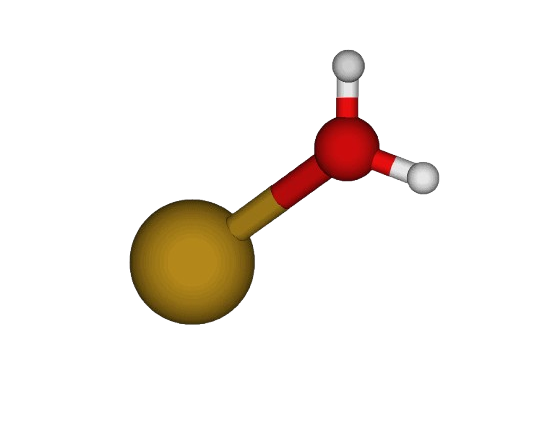
\includegraphics[width=\linewidth]{Imágenes/packmol_agua_01.png}
        \text{$n=1$}
    \end{minipage}\hfill
    \begin{minipage}[b]{0.25\textwidth}
        \centering
        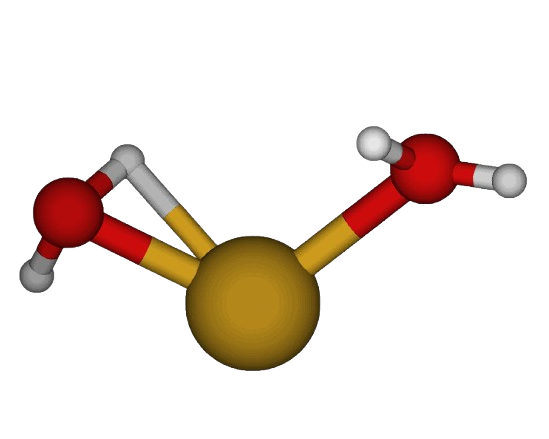
\includegraphics[width=\linewidth]{Imágenes/packmol_agua_02.png}
        \text{$n=2$}
    \end{minipage}\hfill
    \begin{minipage}[b]{0.25\textwidth}
        \centering
        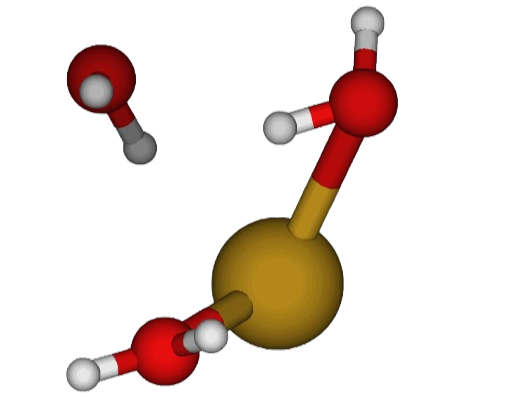
\includegraphics[width=\linewidth]{Imágenes/packmol_agua_03.png}
        \text{$n=3$}
    \end{minipage}
    
    \vspace{0.5cm}

    % --- Fila 2 (n=4, 5, 6) ---
    \begin{minipage}[b]{0.25\textwidth}
        \centering
        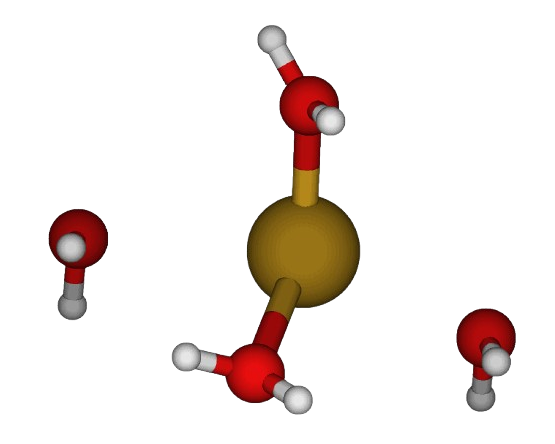
\includegraphics[width=\linewidth]{Imágenes/packmol_agua_04.png}
        \text{$n=4$}
    \end{minipage}\hfill
    \begin{minipage}[b]{0.25\textwidth}
        \centering
        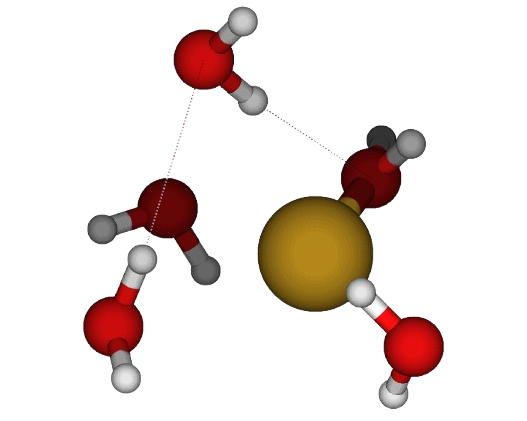
\includegraphics[width=\linewidth]{Imágenes/packmol_agua_05.png}
        \text{$n=5$}
    \end{minipage}\hfill
    \begin{minipage}[b]{0.25\textwidth}
        \centering
        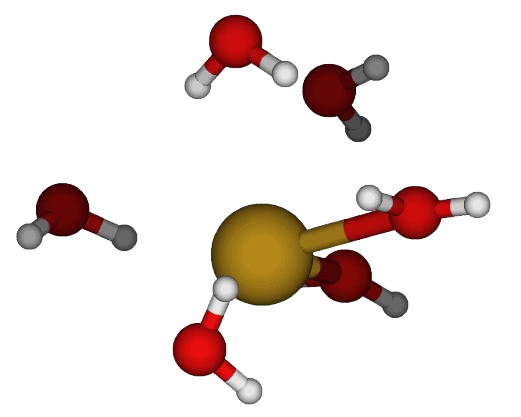
\includegraphics[width=\linewidth]{Imágenes/packmol_agua_06.png}
        \text{$n=6$}
    \end{minipage}

    \vspace{0.5cm}
    
    % --- Fila 3 (n=7, 8, 9) ---
    \begin{minipage}[b]{0.25\textwidth}
        \centering
        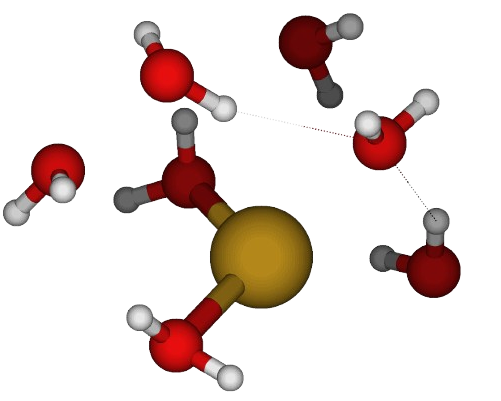
\includegraphics[width=\linewidth]{Imágenes/packmol_agua_07.png}
        \text{$n=7$}
    \end{minipage}\hfill
    \begin{minipage}[b]{0.25\textwidth}
        \centering
        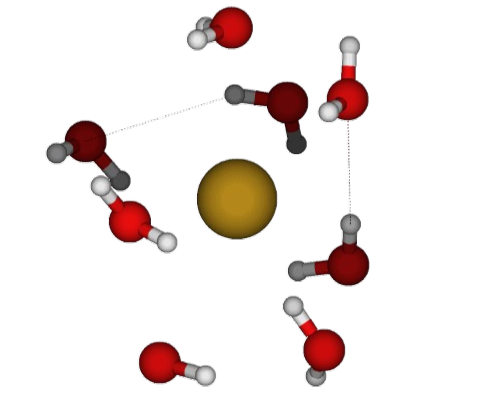
\includegraphics[width=\linewidth]{Imágenes/packmol_agua_08.png}
        \text{$n=8$}
    \end{minipage}\hfill
    \begin{minipage}[b]{0.25\textwidth}
        \centering
        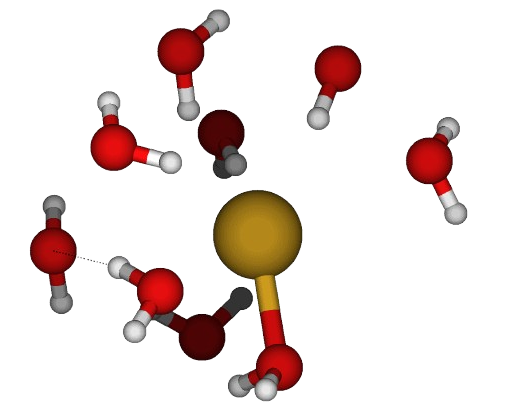
\includegraphics[width=\linewidth]{Imágenes/packmol_agua_09.png}
        \text{$n=9$}
    \end{minipage}

    \vspace{0.5cm}

    % --- Fila 4 (n=10) ---
    \begin{minipage}[b]{0.3\textwidth}
        \centering
        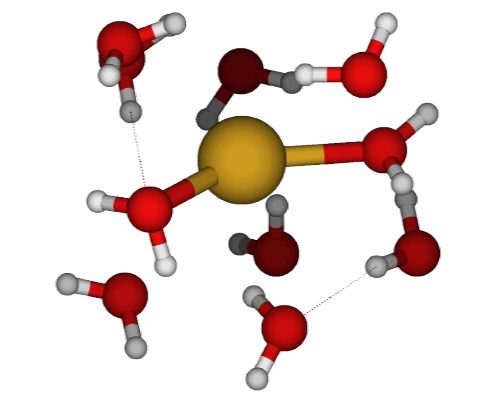
\includegraphics[width=\linewidth]{Imágenes/packmol_agua_10.png}
        \text{$n=10$}
    \end{minipage}
    \caption[Geometrías de partida obtenidas con PACKMOL \ce{[Cu(H2O)_{n}]^{2+}}]{Geometrías de partida para los cúmulos de agua \ce{[Cu(H2O)_{n}]^{2+}} con $n = 1-10$ generadas por optimización geométrica de empaquetamiento con el software PACKMOL \cite{packmol}. Dadas las limitaciones del software, es evidente la falta de interacciones ion-dipolo y la ausencia de un complejo de coordinación definido alrededor del \ce{Cu^{2+}} en estas estructuras iniciales.}
    \label{fig:packmol_agua}
\end{figure}

\begin{figure}[p]
    \centering
    % --- Fila 1 (n=1, 2, 3) ---
    \begin{minipage}[b]{0.25\textwidth}
        \centering
        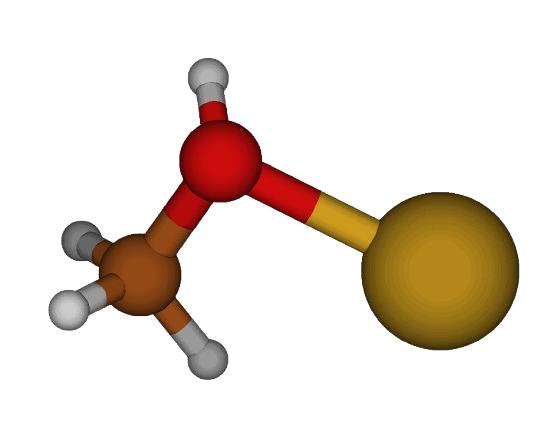
\includegraphics[width=\linewidth]{Imágenes/packmol_metanol_01.png}
        \text{$n=1$}
    \end{minipage}\hfill
    \begin{minipage}[b]{0.25\textwidth}
        \centering
        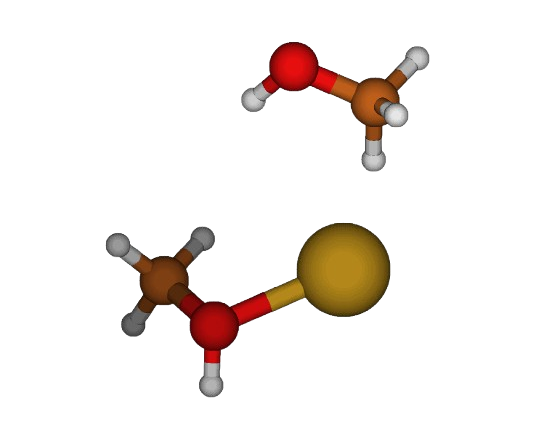
\includegraphics[width=\linewidth]{Imágenes/packmol_metanol_02.png}
        \text{$n=2$}
    \end{minipage}\hfill
    \begin{minipage}[b]{0.25\textwidth}
        \centering
        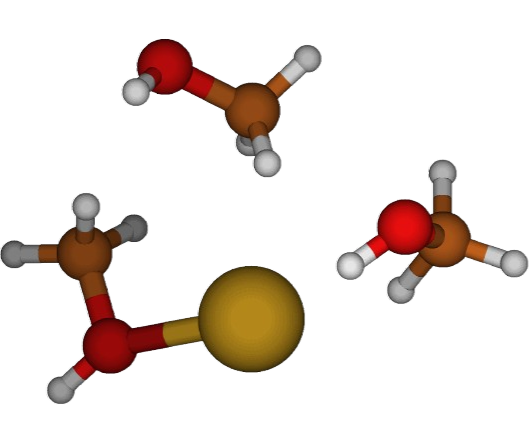
\includegraphics[width=\linewidth]{Imágenes/packmol_metanol_03.png}
        \text{$n=3$}
    \end{minipage}
    
    \vspace{0.5cm}

    % --- Fila 2 (n=4, 5, 6) ---
    \begin{minipage}[b]{0.25\textwidth}
        \centering
        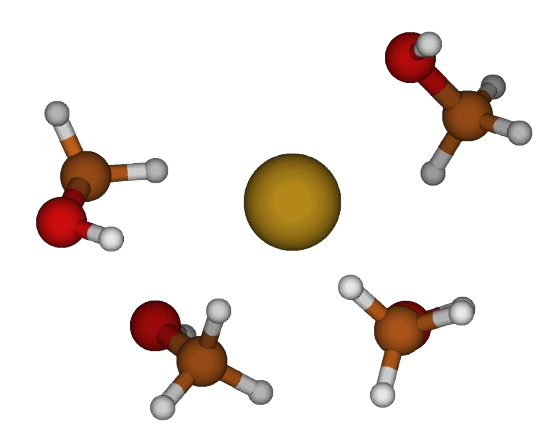
\includegraphics[width=\linewidth]{Imágenes/packmol_metanol_04.png}
        \text{$n=4$}
    \end{minipage}\hfill
    \begin{minipage}[b]{0.25\textwidth}
        \centering
        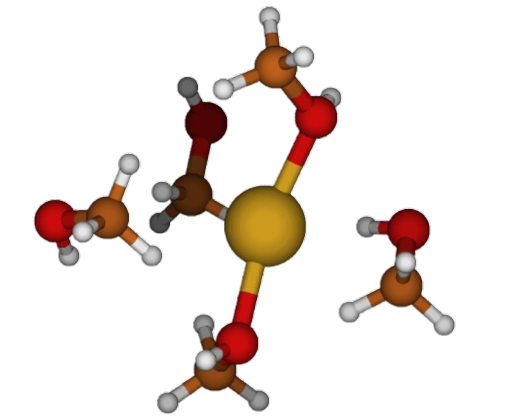
\includegraphics[width=\linewidth]{Imágenes/packmol_metanol_05.png}
        \text{$n=5$}
    \end{minipage}\hfill
    \begin{minipage}[b]{0.25\textwidth}
        \centering
        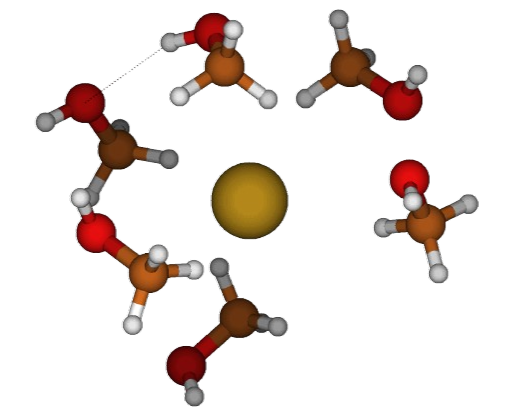
\includegraphics[width=\linewidth]{Imágenes/packmol_metanol_06.png}
        \text{$n=6$}
    \end{minipage}

    \vspace{0.5cm}
    
    % --- Fila 3 (n=7, 8, 9) ---
    \begin{minipage}[b]{0.25\textwidth}
        \centering
        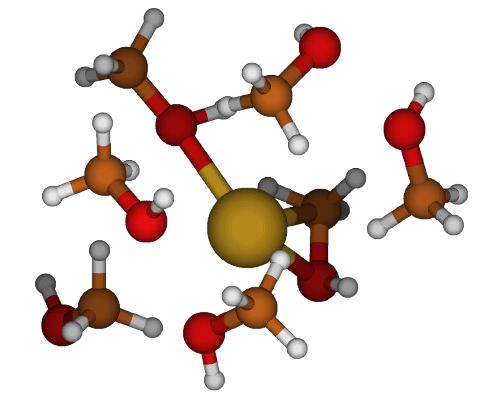
\includegraphics[width=\linewidth]{Imágenes/packmol_metanol_07.png}
        \text{$n=7$}
    \end{minipage}\hfill
    \begin{minipage}[b]{0.25\textwidth}
        \centering
        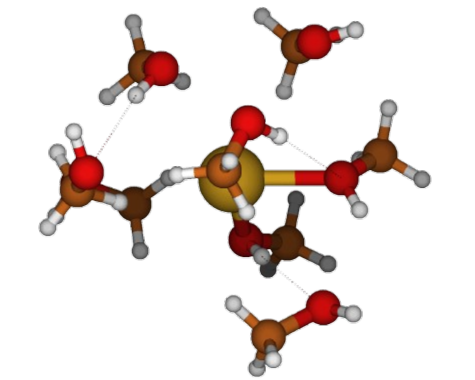
\includegraphics[width=\linewidth]{Imágenes/packmol_metanol_08.png}
        \text{$n=8$}
    \end{minipage}\hfill
    \begin{minipage}[b]{0.25\textwidth}
        \centering
        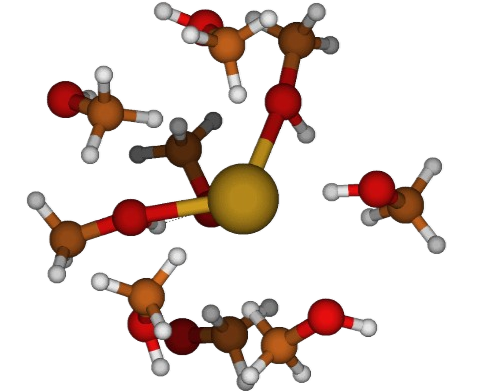
\includegraphics[width=\linewidth]{Imágenes/packmol_metanol_09.png}
        \text{$n=9$}
    \end{minipage}

    \vspace{0.5cm}

    % --- Fila 4 (n=10) ---
    \begin{minipage}[b]{0.3\textwidth}
        \centering
        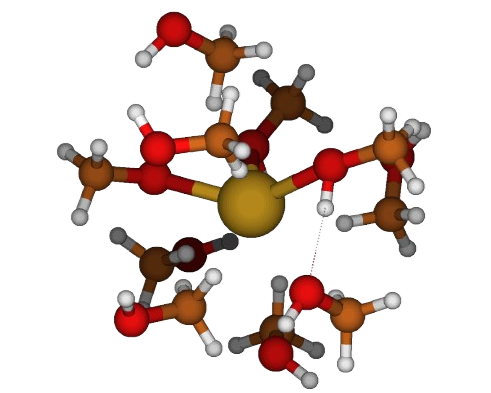
\includegraphics[width=\linewidth]{Imágenes/packmol_metanol_10.png}
        \text{$n=10$}
    \end{minipage}
    \caption[Geometrías de partida obtenidas con PACKMOL \ce{[Cu(CH4O)_{n}]^{2+}}]{Geometrías de partida para los cúmulos de metanol \ce{[Cu(CH4O)_{n}]^{2+}} con $n = 1-10$ generadas por optimización geométrica de empaquetamiento con el software PACKMOL \cite{packmol}. Dadas las limitaciones del software, es evidente la falta de interacciones ion-dipolo y la ausencia de un complejo de coordinación definido alrededor del \ce{Cu^{2+}} en estas estructuras iniciales.}
    \label{fig:packmol_metanol}
\end{figure}

Es importante destacar que estas geometrías obedecen a principios puramente geométricos y no a interacciones físicas explícitas, como momentos dipolares o puentes de hidrógeno. Esto se debe a que PACKMOL no emplea campos de fuerza ni potenciales químicos; en su lugar, aborda el posicionamiento como un problema de optimización donde se minimiza una función de mérito $f(\mathbf{c}, \mathbf{\theta})$ sujeta a restricciones espaciales y a una tolerancia de distancia interatómica $d_{tol}$ \cite{packmol}. En esta formulación, el vector $\mathbf{c}$ representa el desplazamiento de los baricentros de las moléculas hacia sus posiciones finales en el espacio tridimensional, mientras que el parámetro $\mathbf{\theta}$ define los ángulos de rotación que determinan la orientación espacial de cada unidad molecular. Mediante el ajuste iterativo de estas variables, el software desplaza y rota las moléculas de manera independiente hasta alcanzar un estado donde la función de mérito se anula ($f=0$). Por consiguiente, aunque el algoritmo evita eficazmente el solapamiento atómico, las configuraciones resultantes carecen de un equilibrio termodinámico real y no representan de ninguna manera estructuras de mínima energía realistas. 

\subsubsection*{Optimización}
Posterior a la generación de dichas geometrías, se procedió a la optimización empleando el software ORCA v6.1 \cite{orca,orca6.1}. El funcional de intercambio y correlación utilizado es el híbrido meta-GGA M06-2X, el cual se complementó con la corrección de dispersión de Grimme (D3(0)) para capturar las interacciones de dispersión de largo alcance entre las moléculas de solvente, evitando el doble conteo de energía en el rango corto mediante una función de amortiguamiento a cero \cite{grimme2010consistent}. Para los átomos ligeros constituyentes del solvente (H, C y O), se evaluó el desempeño de las bases Pople 6-31G*, 6-31+G* y 6-31++G**, de manera que se evaluó el impacto en el incremento de funciones de polarización y funciones difusas (se discutirá más a detalle en la siguiente sección). Para el ion \ce{Cu^{2+}}, se empleó el pseudopotencial efectivo de carozo (ECP, por sus siglas en inglés) de la serie de Stuttgart-Cologne, específicamente el MDF10 \cite{figgen2005energy}. Este pseudopotencial de ``carozo pequeño'' sustituye los 10 electrones internos ($1s^2 2s^2 2p^6$), incorporando efectos relativistas de manera implícita mediante un ajuste previo a datos de cálculos atómicos multiconfiguracionales de Dirac-Hartree-Fock. El uso de este ECP no solo reduce el costo computacional, sino que permite tratar de manera explícita los 19 electrones restantes ($3s$, $3p$, $3d$ y $4s$), capturando así la polarización del carozo externo y su influencia en la geometría de coordinación. Complementando al ECP, se utilizó el conjunto de bases de correlación-consistente aug-cc-pVDZ-PP desarrollado por Peterson y Puzzarini \cite{peterson2005systematically}. Esta base está diseñada específicamente para ser compatible con pseudopotenciales relativistas e incluye funciones difusas (augmented) y de polarización.
Finalmente, todos los cálculos se realizaron bajo un nivel de integración numérica DEFGRID3, considerando un estado de capa abierta tipo doblete (carga +2 y multiplicidad 2) correspondiente a la configuración electrónica $d^9$ del ion \ce{Cu^{2+}}. Tras cada optimización de geometría, se ejecutó un análisis de frecuencias vibracionales con el objetivo de confirmar que las estructuras obtenidas representan mínimos verdaderos en la superficie de energía potencial.

Todas las geometrías optimizadas desde $n = 1$ hasta $n = 10$ con la base 6-31G* se muestran en la figura \ref{fig:geo_opt_cumulos} para los cúmulos de agua y en la figura \ref{fig:geo_opt_cumulos_m} para los cúmulos de metanol.

\begin{figure}[H]
    \centering
    % --- Fila 1 (n=1, 2, 3) ---
    \begin{minipage}[b]{0.25\textwidth}
        \centering
        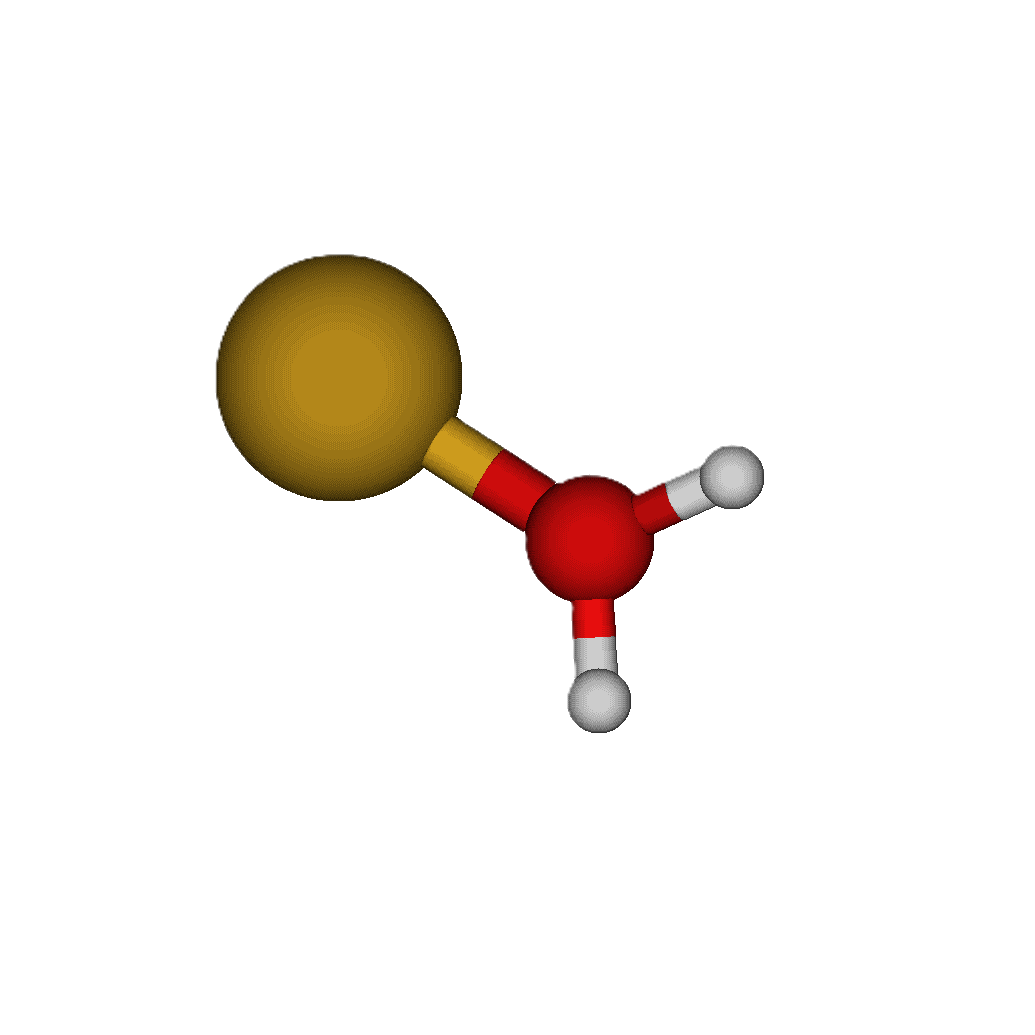
\includegraphics[width=\linewidth]{Imágenes/geometria_opt_n_1.png}
        \text{$n=1$}
    \end{minipage}\hfill
    \begin{minipage}[b]{0.25\textwidth}
        \centering
        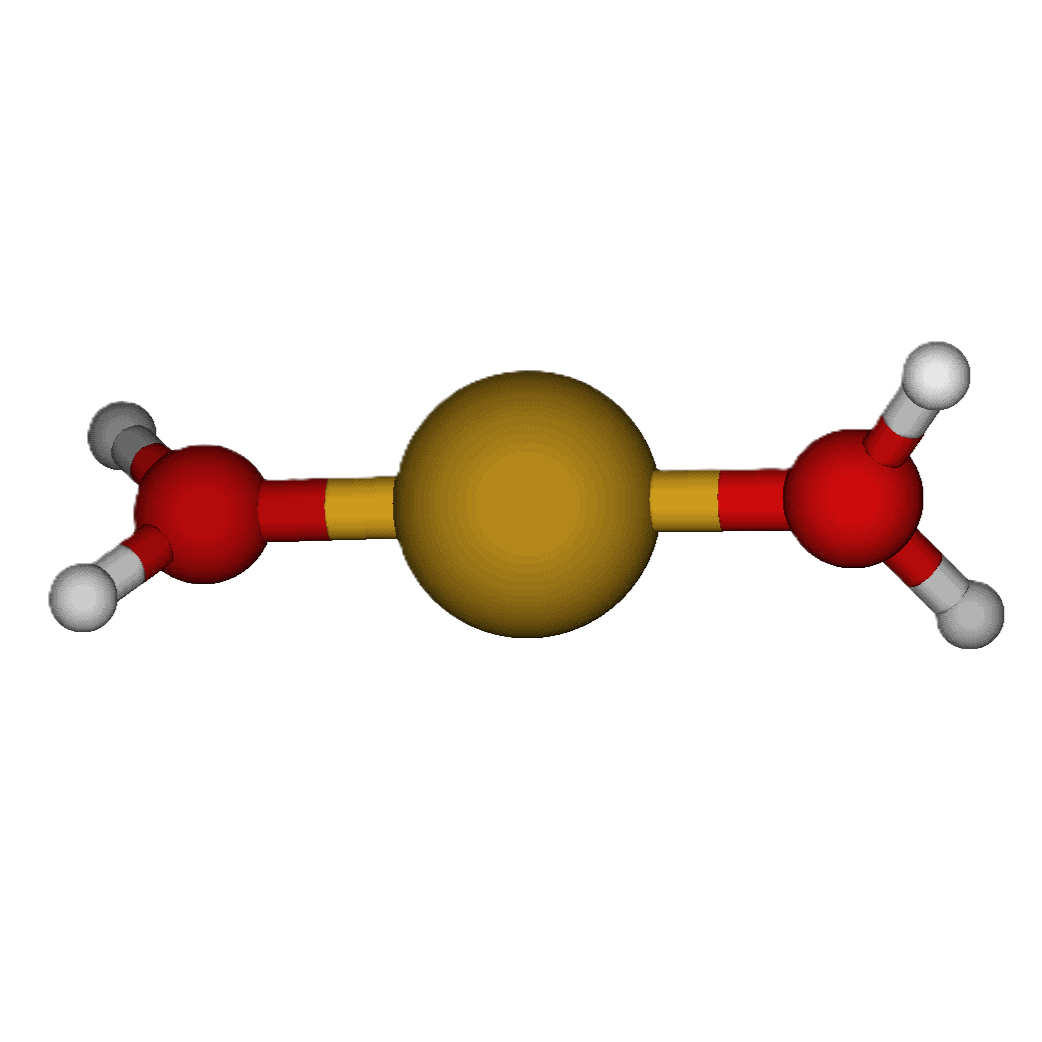
\includegraphics[width=\linewidth]{Imágenes/geometria_opt_n_2.png}
        \text{$n=2$}
    \end{minipage}\hfill
    \begin{minipage}[b]{0.25\textwidth}
        \centering
        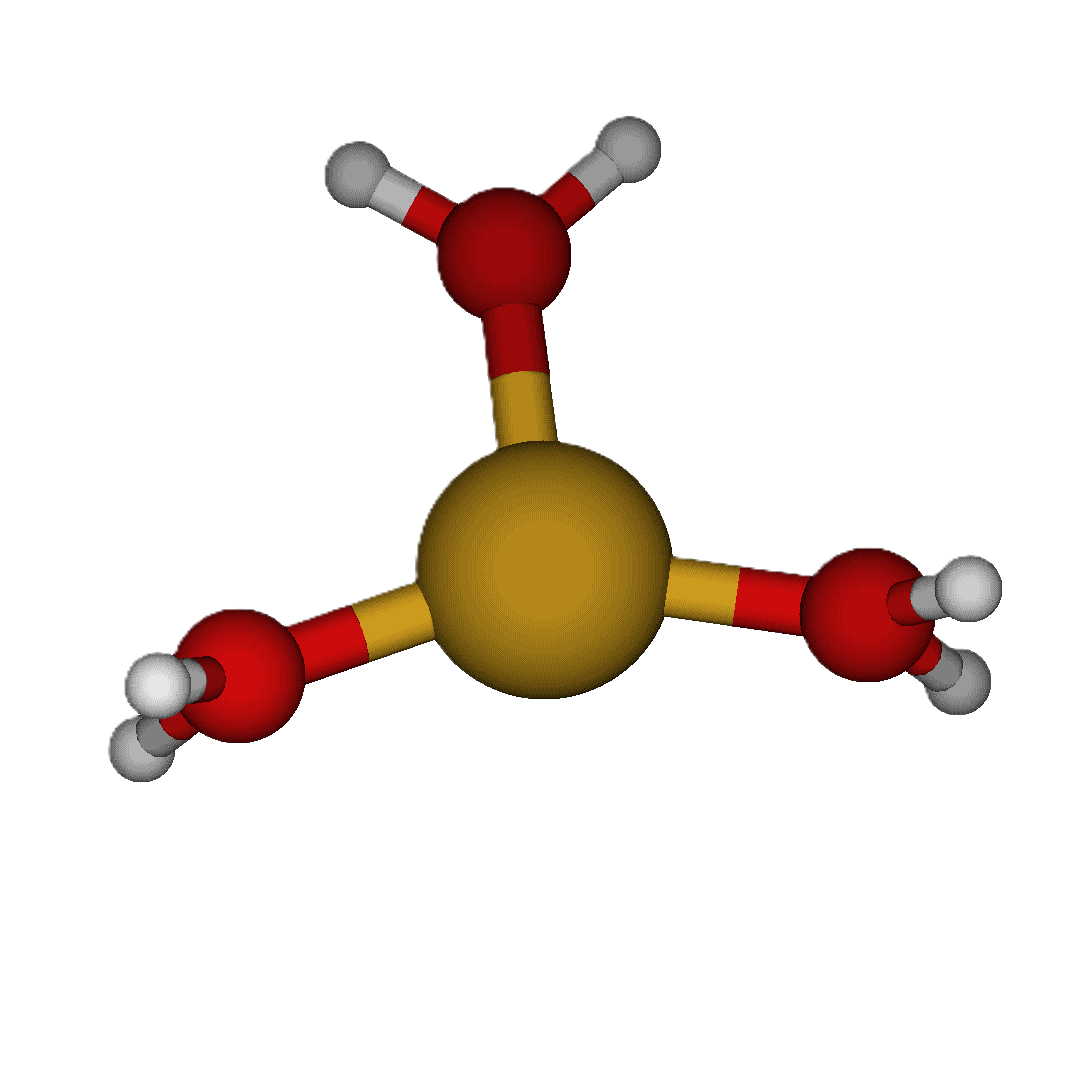
\includegraphics[width=\linewidth]{Imágenes/geometria_opt_n_3.png}
        \text{$n=3$}
    \end{minipage}
    
    \vspace{0.5cm} % Espacio vertical entre filas

    % --- Fila 2 (n=4, 5, 6) ---
    \begin{minipage}[b]{0.25\textwidth}
        \centering
        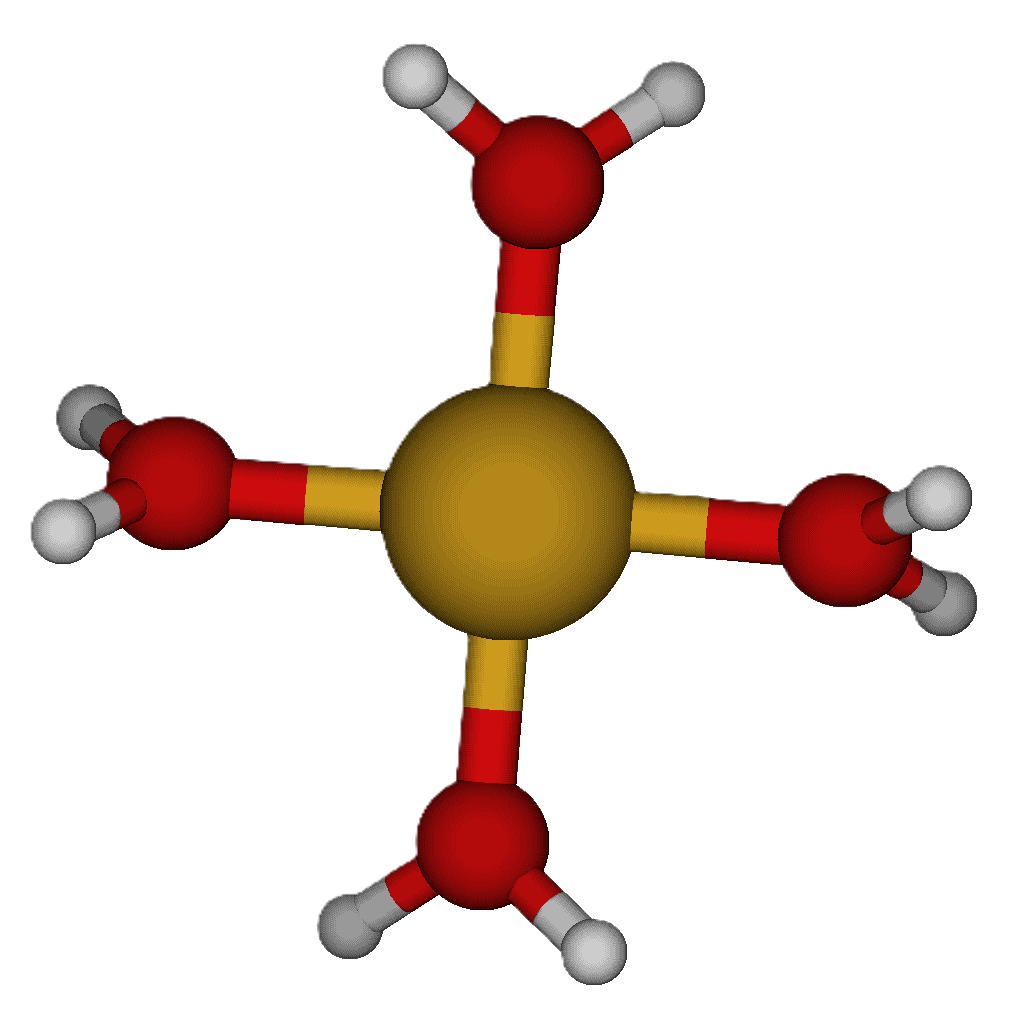
\includegraphics[width=\linewidth]{Imágenes/geometria_opt_n_4.png}
        \text{$n=4$}
    \end{minipage}\hfill
    \begin{minipage}[b]{0.25\textwidth}
        \centering
        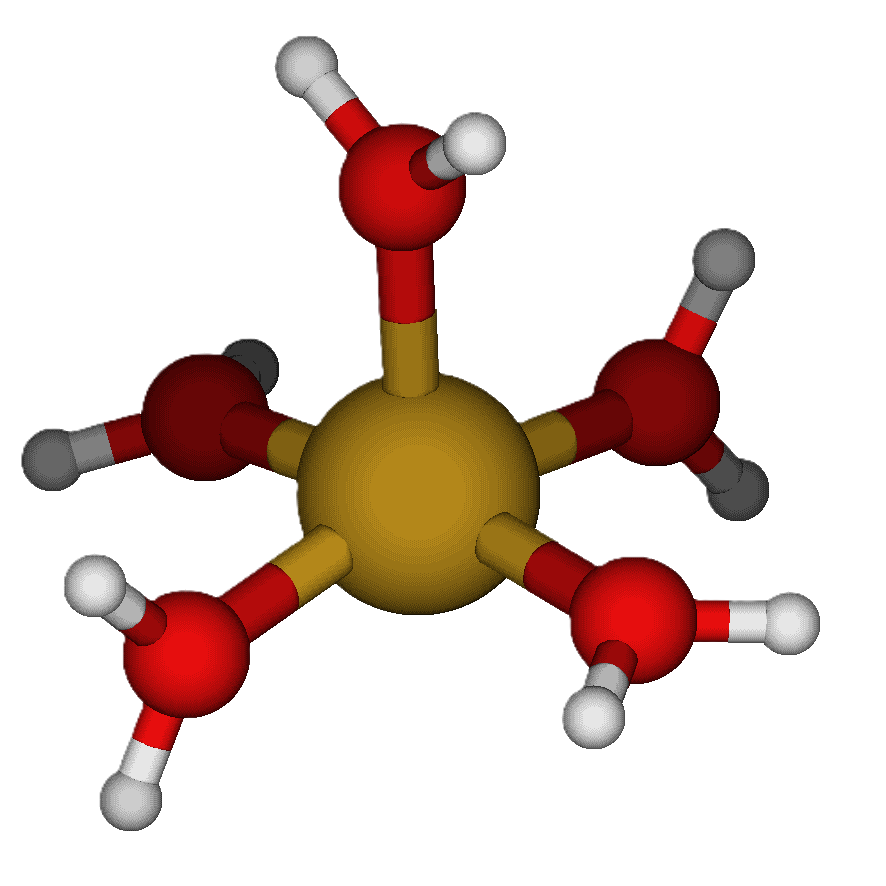
\includegraphics[width=\linewidth]{Imágenes/geometria_opt_n_5.png}
        \text{$n=5$}
    \end{minipage}\hfill
    \begin{minipage}[b]{0.25\textwidth}
        \centering
        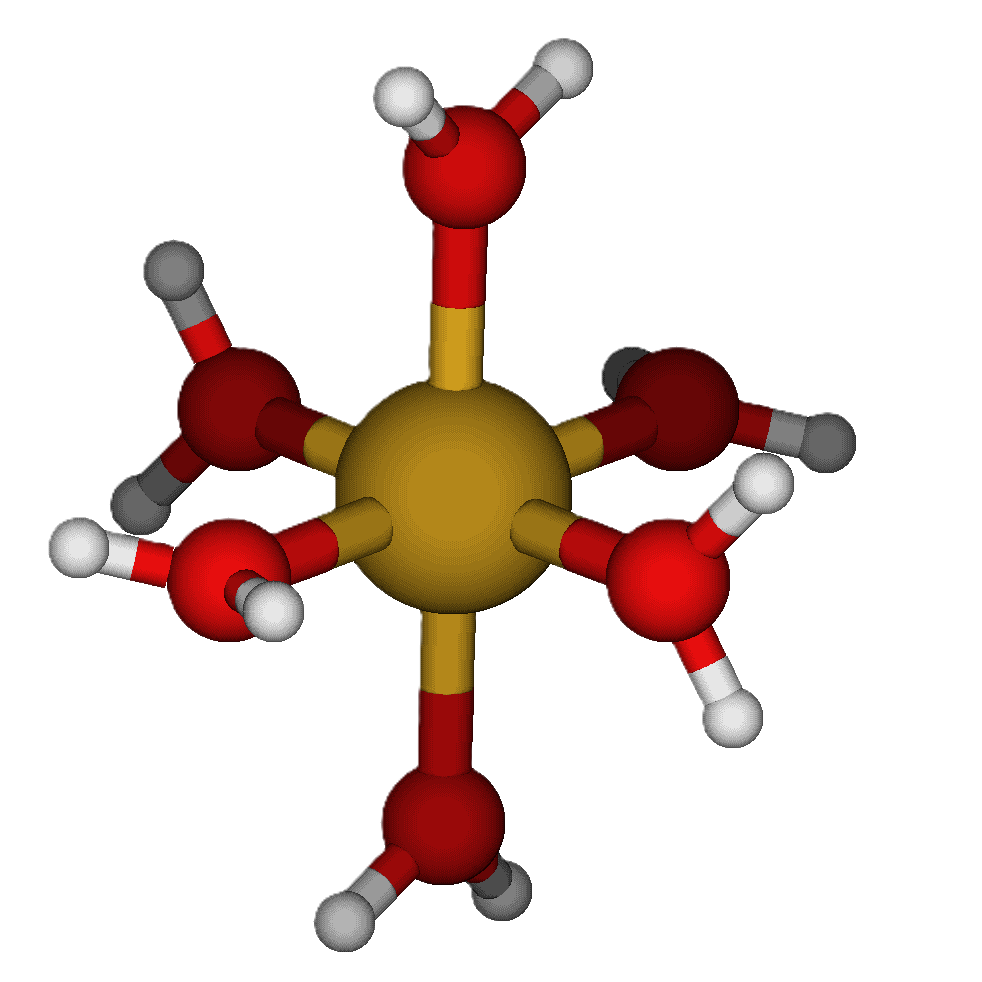
\includegraphics[width=\linewidth]{Imágenes/geometria_opt_n_6.png}
        \text{$n=6$}
    \end{minipage}

    \vspace{0.5cm} % Espacio vertical entre filas
    
    % --- Fila 3 (n=7, 8, 9) ---
    \begin{minipage}[b]{0.25\textwidth}
        \centering
        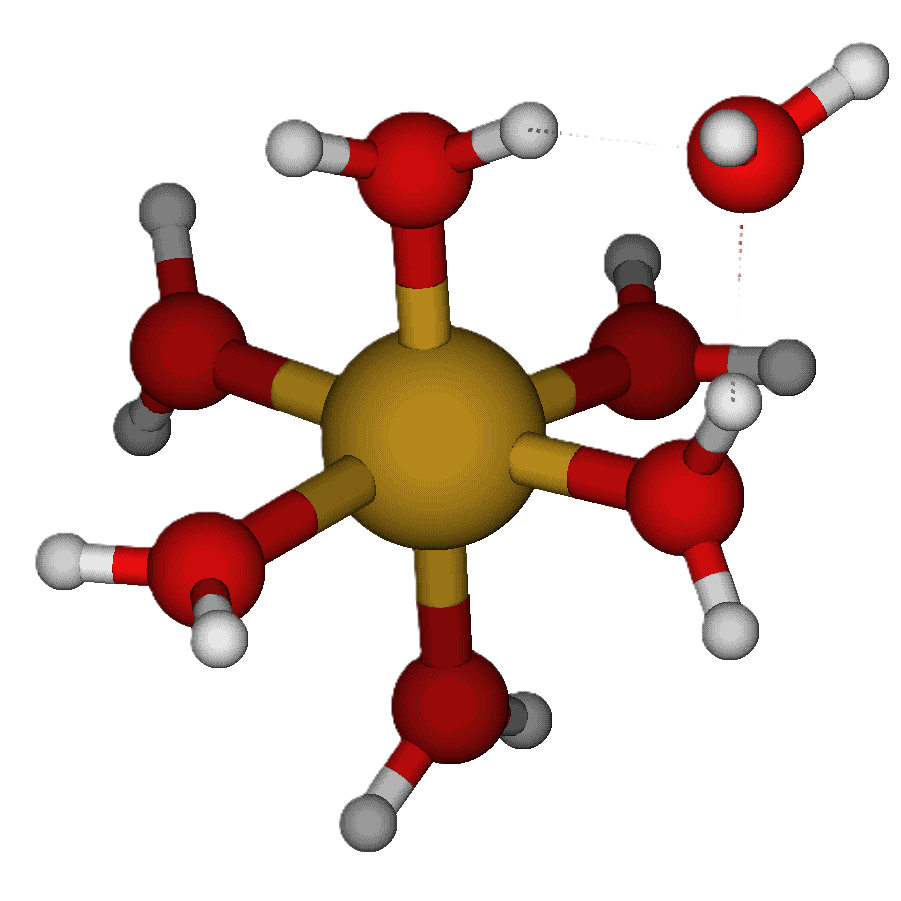
\includegraphics[width=\linewidth]{Imágenes/geometria_opt_n_7.png}
        \text{$n=7$}
    \end{minipage}\hfill
    \begin{minipage}[b]{0.25\textwidth}
        \centering
        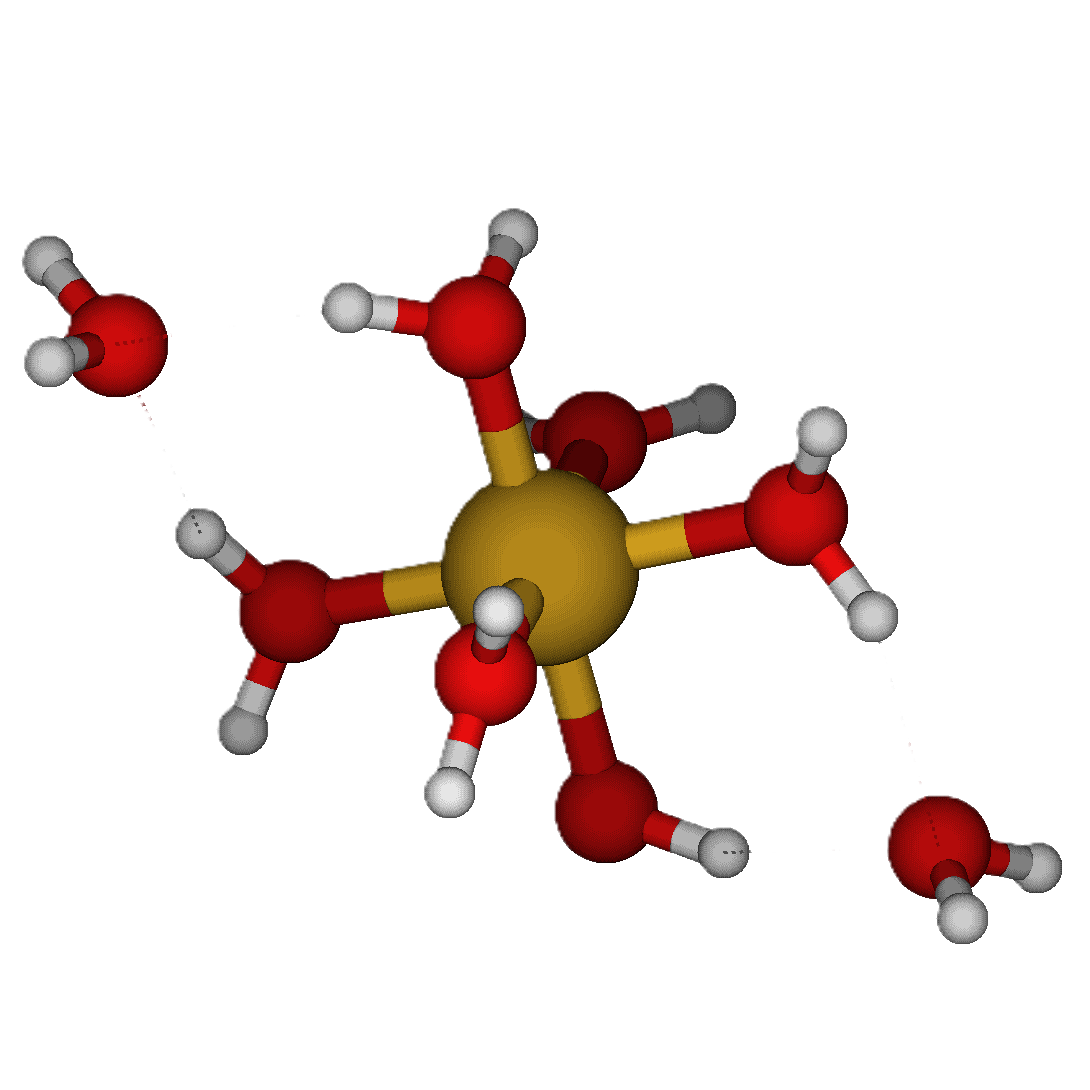
\includegraphics[width=\linewidth]{Imágenes/geometria_opt_n_8.png}
        \text{$n=8$}
    \end{minipage}\hfill
    \begin{minipage}[b]{0.25\textwidth}
        \centering
        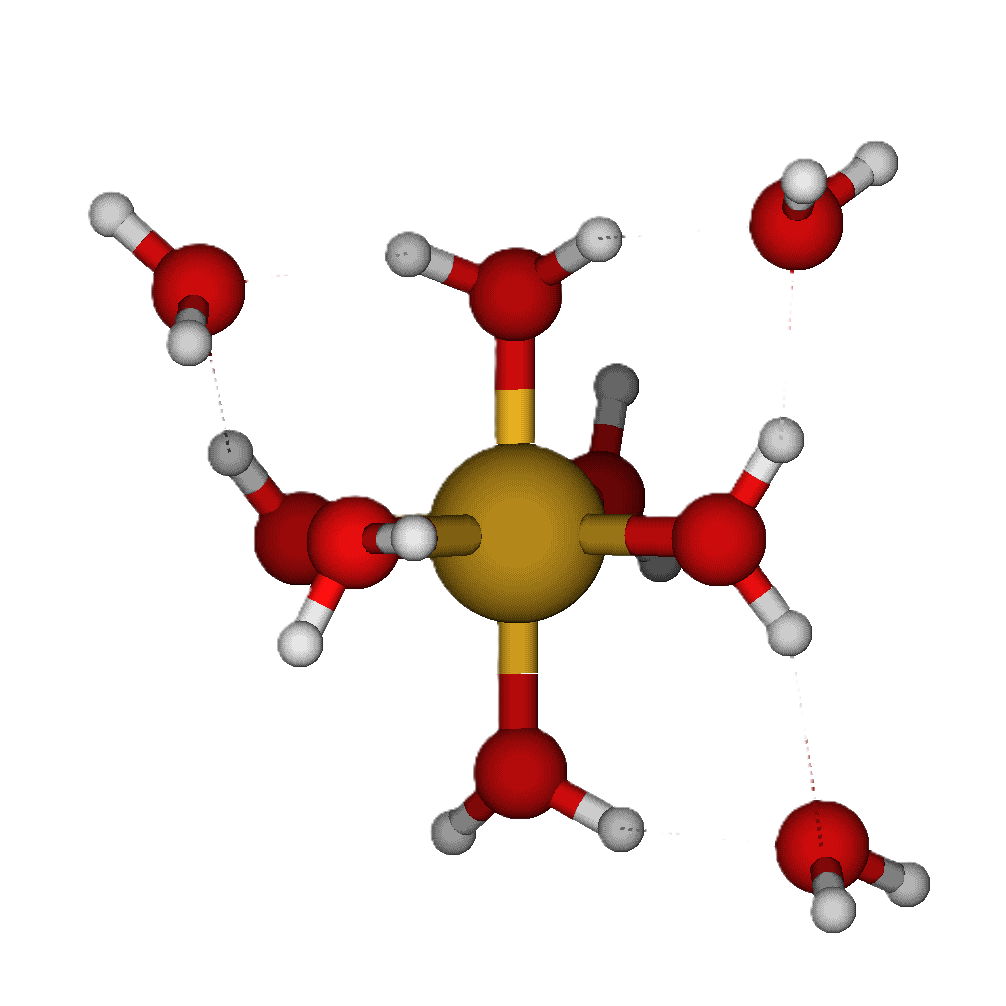
\includegraphics[width=\linewidth]{Imágenes/geometria_opt_n_9.png}
        \text{$n=9$}
    \end{minipage}

    \vspace{0.5cm} % Espacio vertical entre filas

    % --- Fila 4 (n=10, 30, 40) ---
    \begin{minipage}[b]{0.3\textwidth}
        \centering
        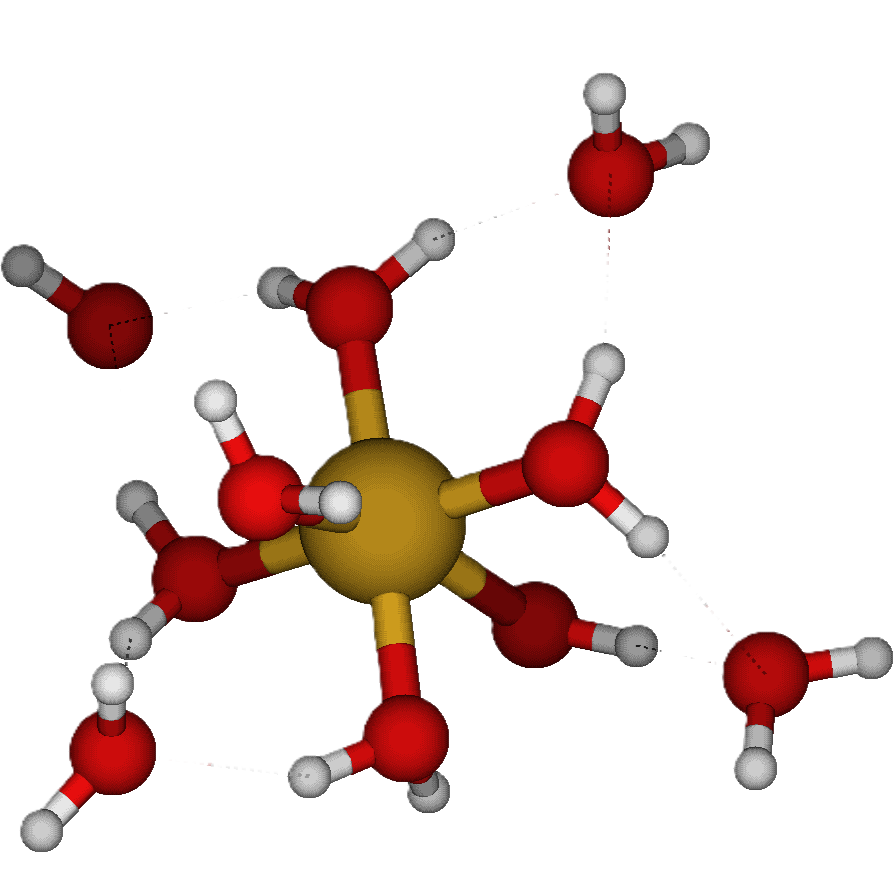
\includegraphics[width=\linewidth]{Imágenes/geometria_opt_n_10.png}
        \text{$n=10$}
    \end{minipage}\hfill
    \begin{minipage}[b]{0.3\textwidth}
        \centering
        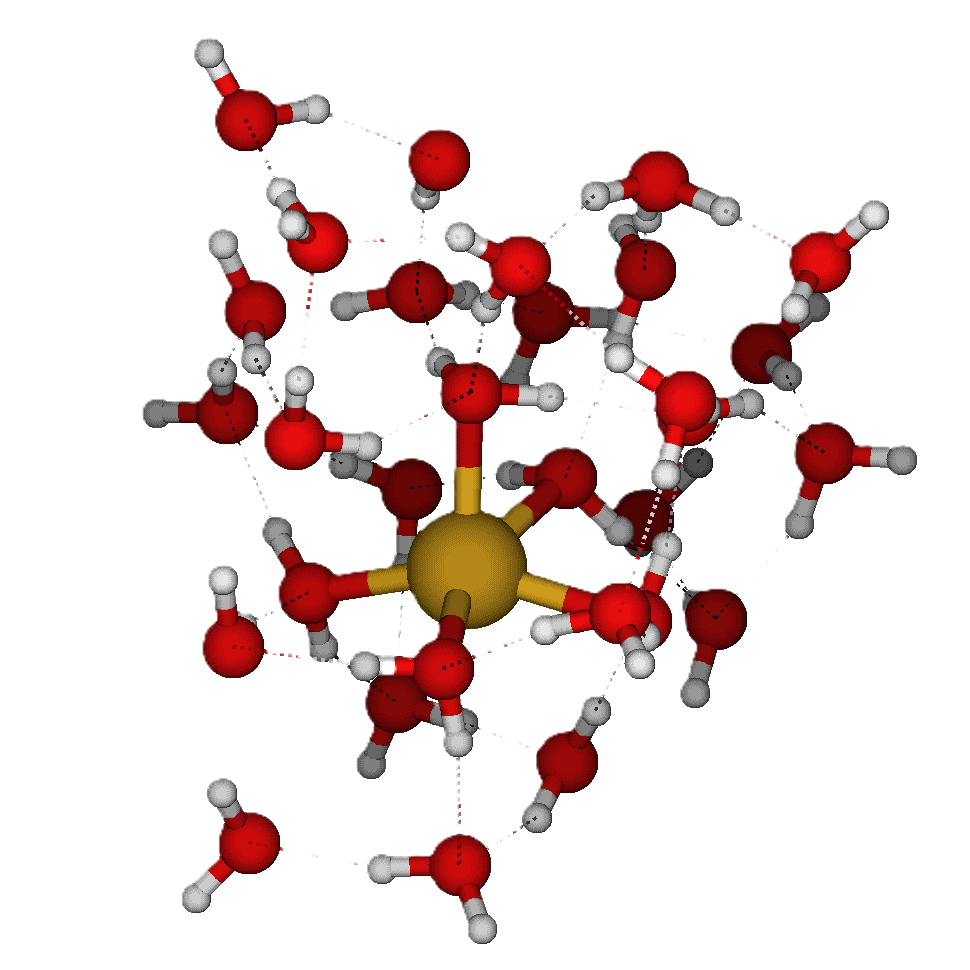
\includegraphics[width=\linewidth]{Imágenes/geometria_opt_n_30.png}
        \text{$n=30$}
    \end{minipage}\hfill
    \begin{minipage}[b]{0.3\textwidth}
        \centering
        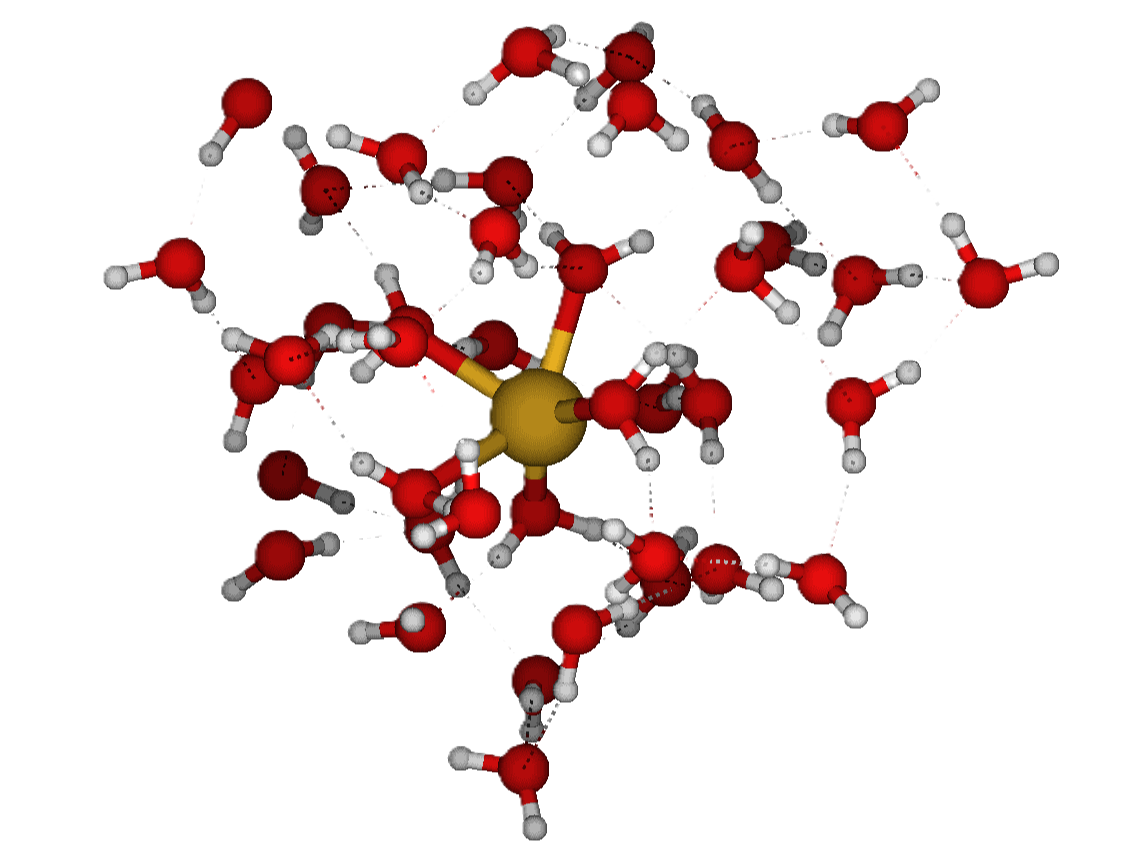
\includegraphics[width=\linewidth]{Imágenes/geometria_opt_n_40.png}
        \text{$n=40$}
    \end{minipage}
    \caption[Geometrías optimizadas obtenidas con M06-2X/6-31G* \ce{[Cu(H2O)_{n}]^{2+}} ]{Geometrías optimizadas para los cúmulos \ce{[Cu(H2O)_{n}]^{2+}} con $n = 1-10, 30, 40$ en el nivel de teoría M06-2X/6-31G*.}
    \label{fig:geo_opt_cumulos}
\end{figure}

\begin{figure}[H]
    \centering
    % --- Fila 1 (n=1, 2, 3) ---
    \begin{minipage}[b]{0.25\textwidth}
        \centering
        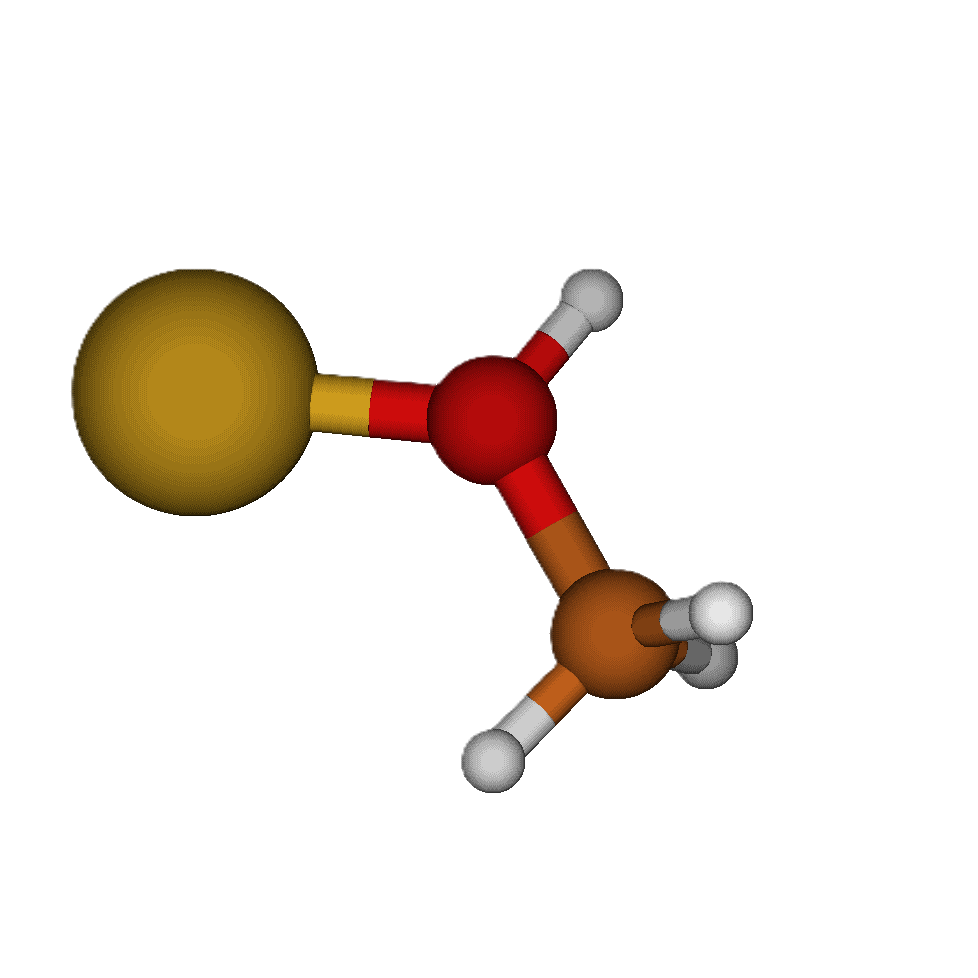
\includegraphics[width=\linewidth]{Imágenes/m_geometria_opt_n_1.png}
        \text{$n=1$}
    \end{minipage}\hfill
    \begin{minipage}[b]{0.25\textwidth}
        \centering
        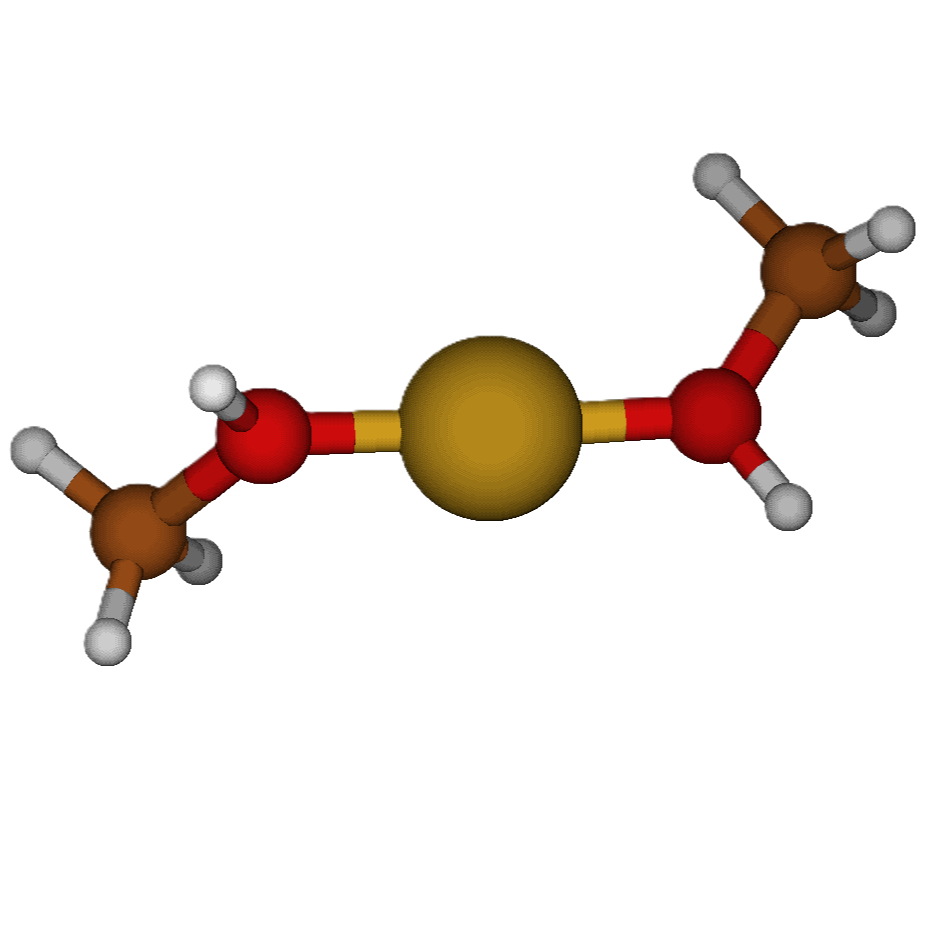
\includegraphics[width=\linewidth]{Imágenes/m_geometria_opt_n_2.png}
        \text{$n=2$}
    \end{minipage}\hfill
    \begin{minipage}[b]{0.25\textwidth}
        \centering
        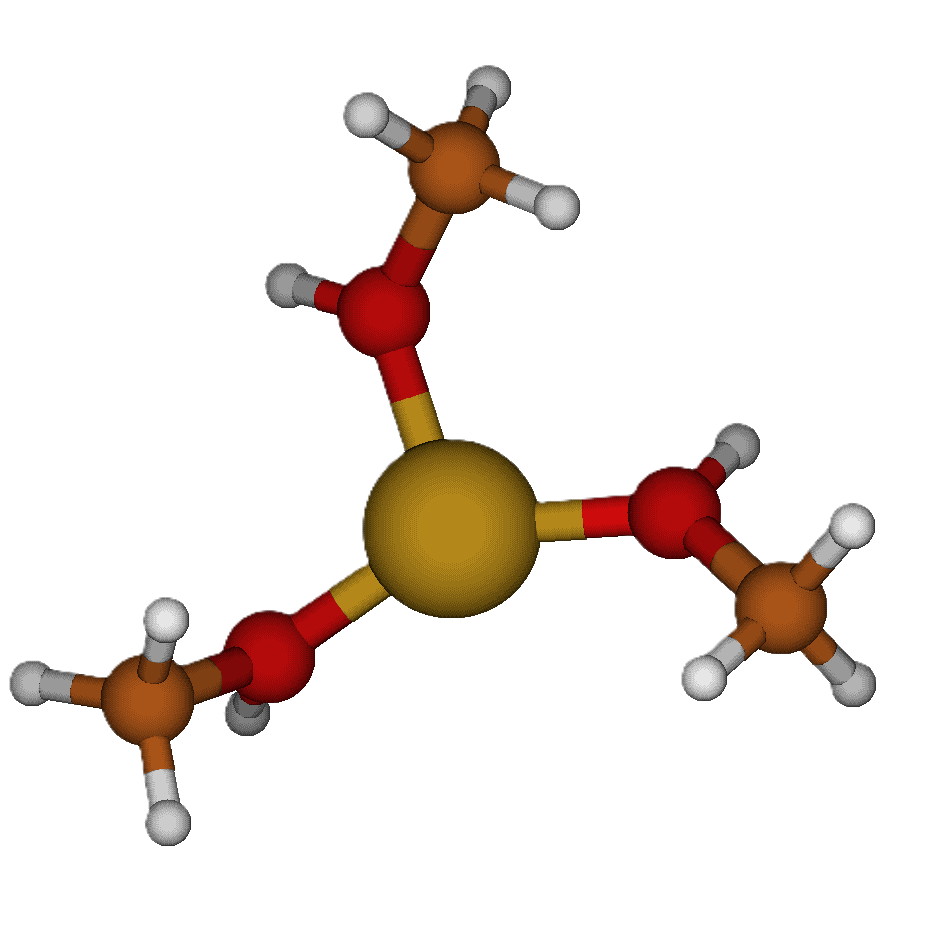
\includegraphics[width=\linewidth]{Imágenes/m_geometria_opt_n_3.png}
        \text{$n=3$}
    \end{minipage}
    
    \vspace{0.5cm} % Espacio vertical entre filas

    % --- Fila 2 (n=4, 5, 6) ---
    \begin{minipage}[b]{0.25\textwidth}
        \centering
        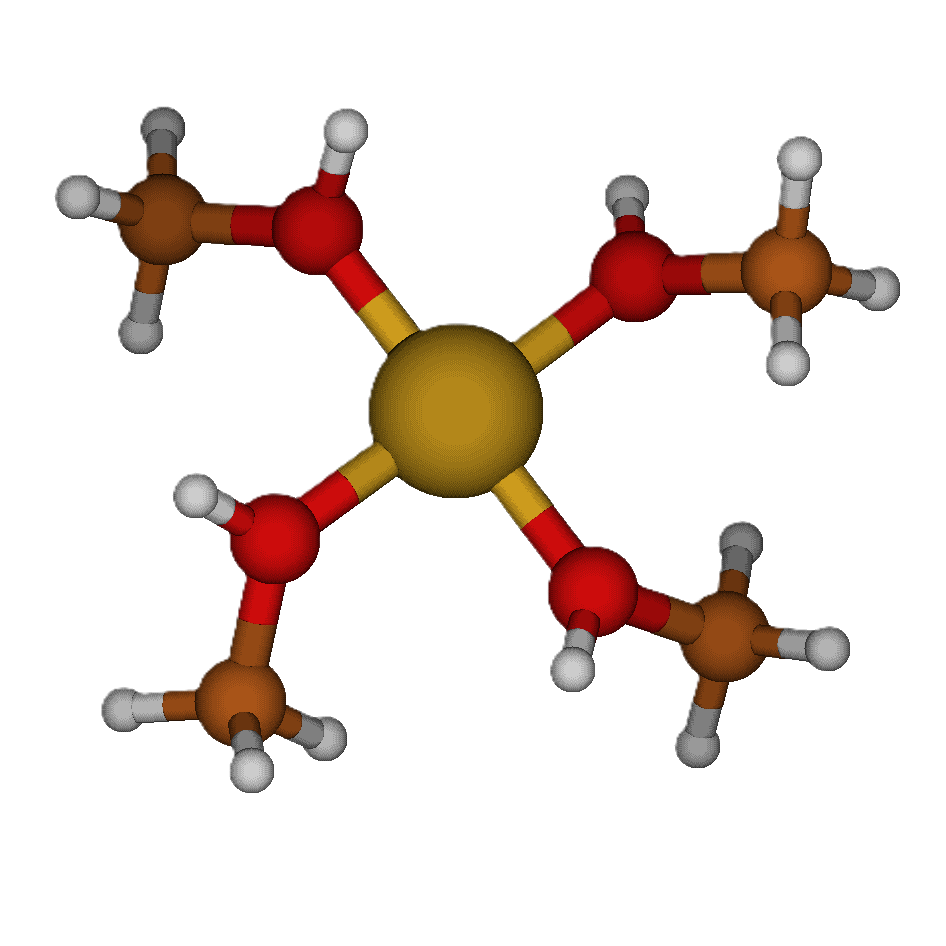
\includegraphics[width=\linewidth]{Imágenes/m_geometria_opt_n_4.png}
        \text{$n=4$}
    \end{minipage}\hfill
    \begin{minipage}[b]{0.25\textwidth}
        \centering
        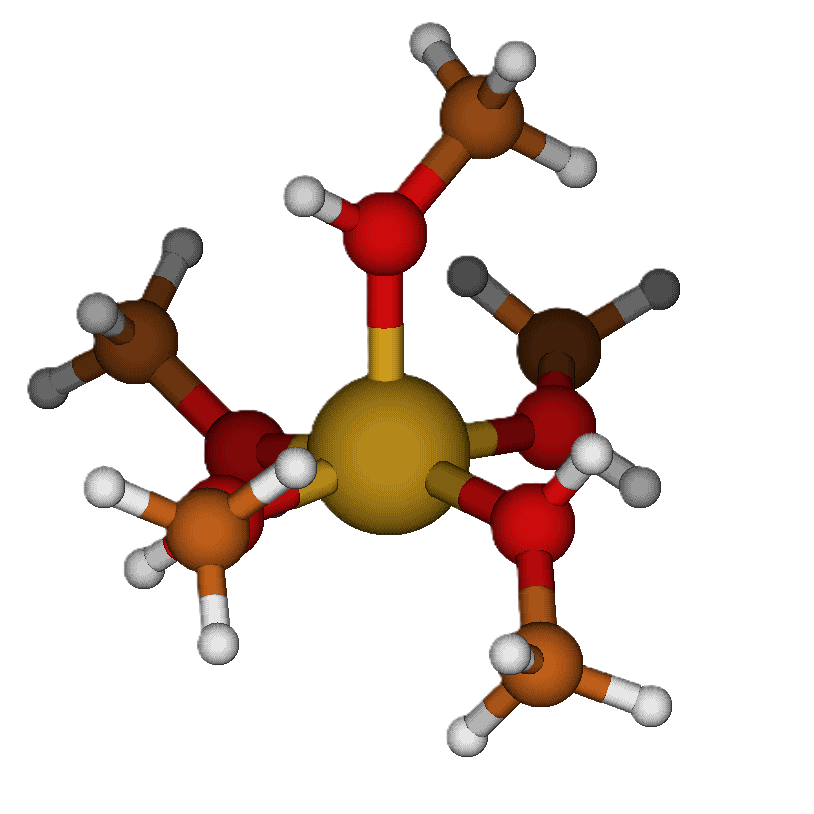
\includegraphics[width=\linewidth]{Imágenes/m_geometria_opt_n_5.png}
        \text{$n=5$}
    \end{minipage}\hfill
    \begin{minipage}[b]{0.25\textwidth}
        \centering
        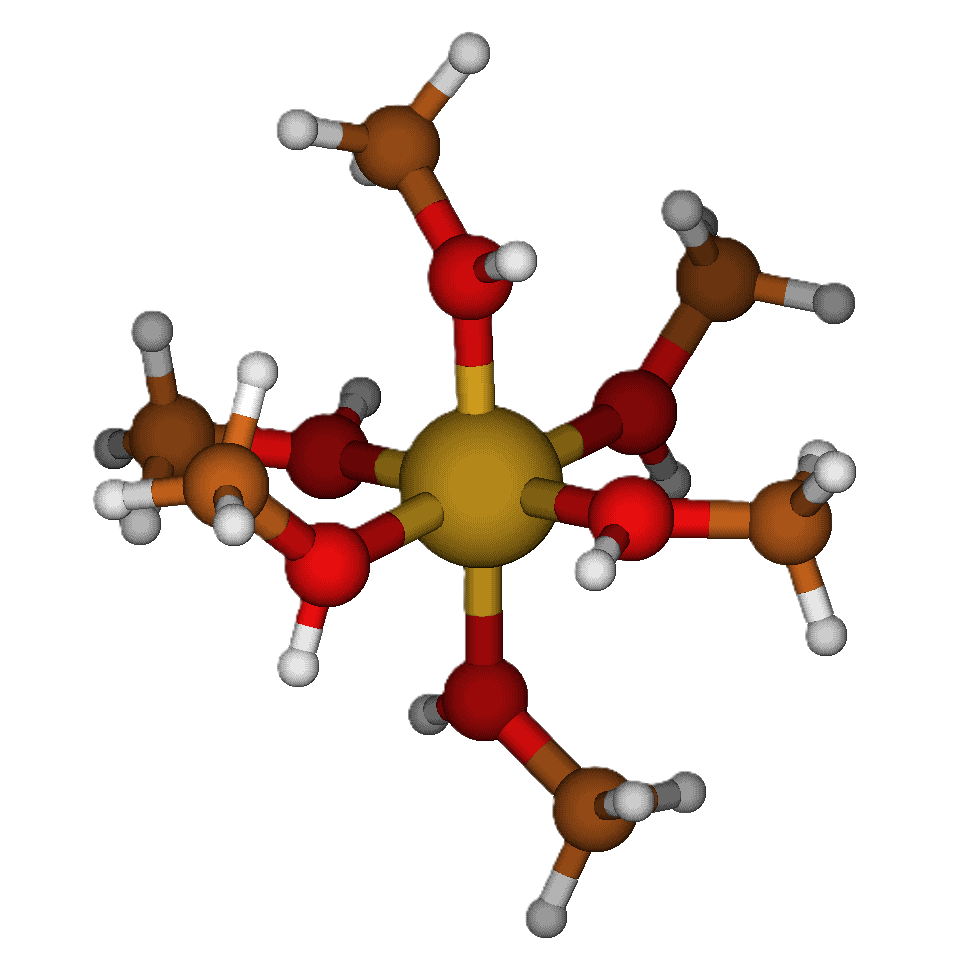
\includegraphics[width=\linewidth]{Imágenes/m_geometria_opt_n_6.png}
        \text{$n=6$}
    \end{minipage}

    \vspace{0.5cm} % Espacio vertical entre filas
    
    % --- Fila 3 (n=7, 8, 9) ---
    \begin{minipage}[b]{0.25\textwidth}
        \centering
        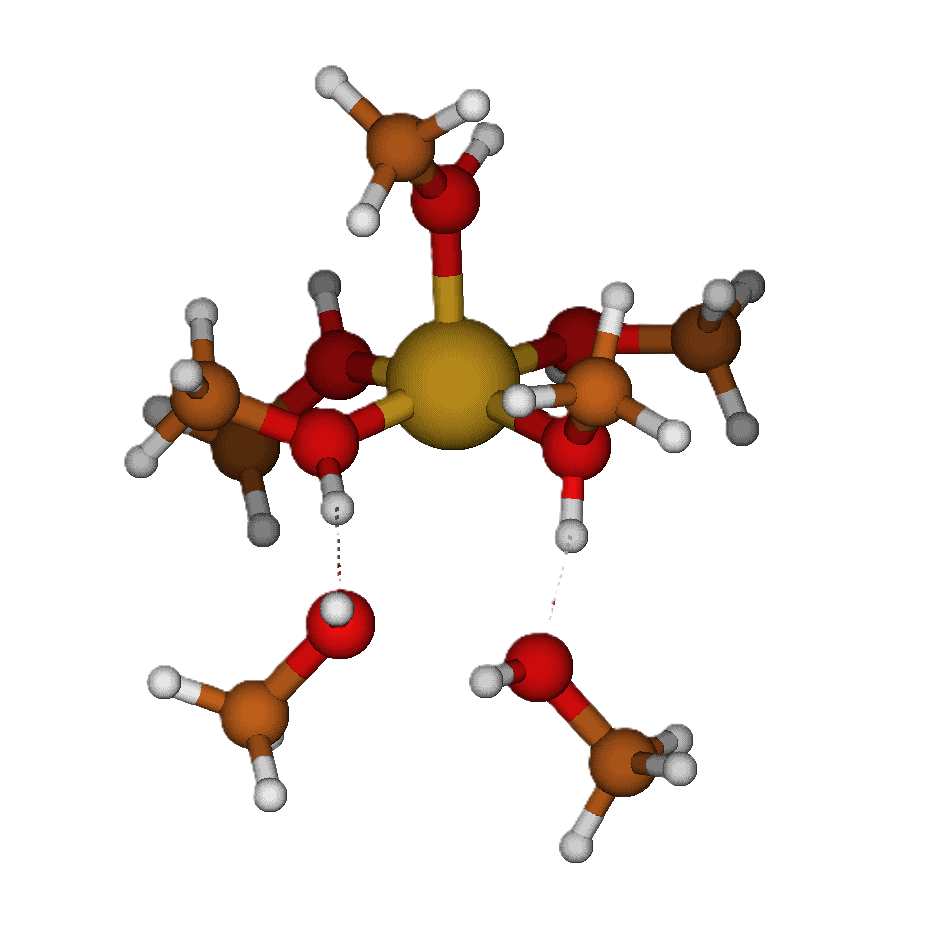
\includegraphics[width=\linewidth]{Imágenes/m_geometria_opt_n_7.png}
        \text{$n=7$}
    \end{minipage}\hfill
    \begin{minipage}[b]{0.25\textwidth}
        \centering
        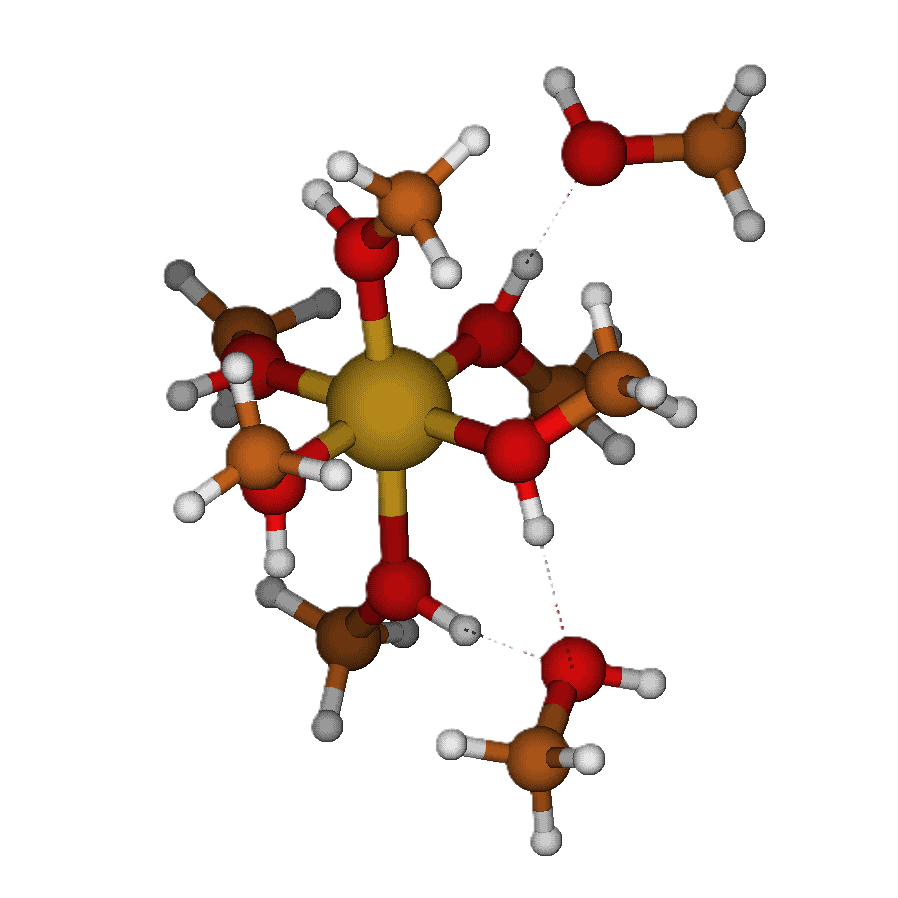
\includegraphics[width=\linewidth]{Imágenes/m_geometria_opt_n_8.png}
        \text{$n=8$}
    \end{minipage}\hfill
    \begin{minipage}[b]{0.25\textwidth}
        \centering
        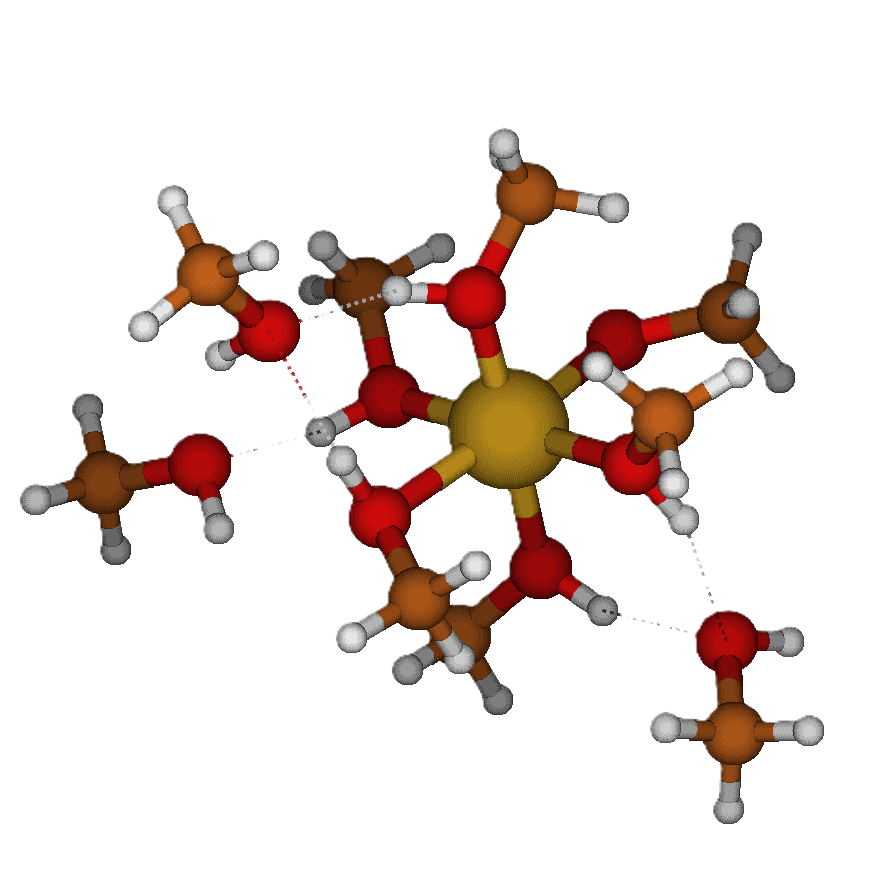
\includegraphics[width=\linewidth]{Imágenes/m_geometria_opt_n_9.png}
        \text{$n=9$}
    \end{minipage}

    \vspace{0.5cm} % Espacio vertical entre filas

    % --- Fila 4 (n=10, 30, 40) ---
    \begin{minipage}[b]{0.3\textwidth}
        \centering
        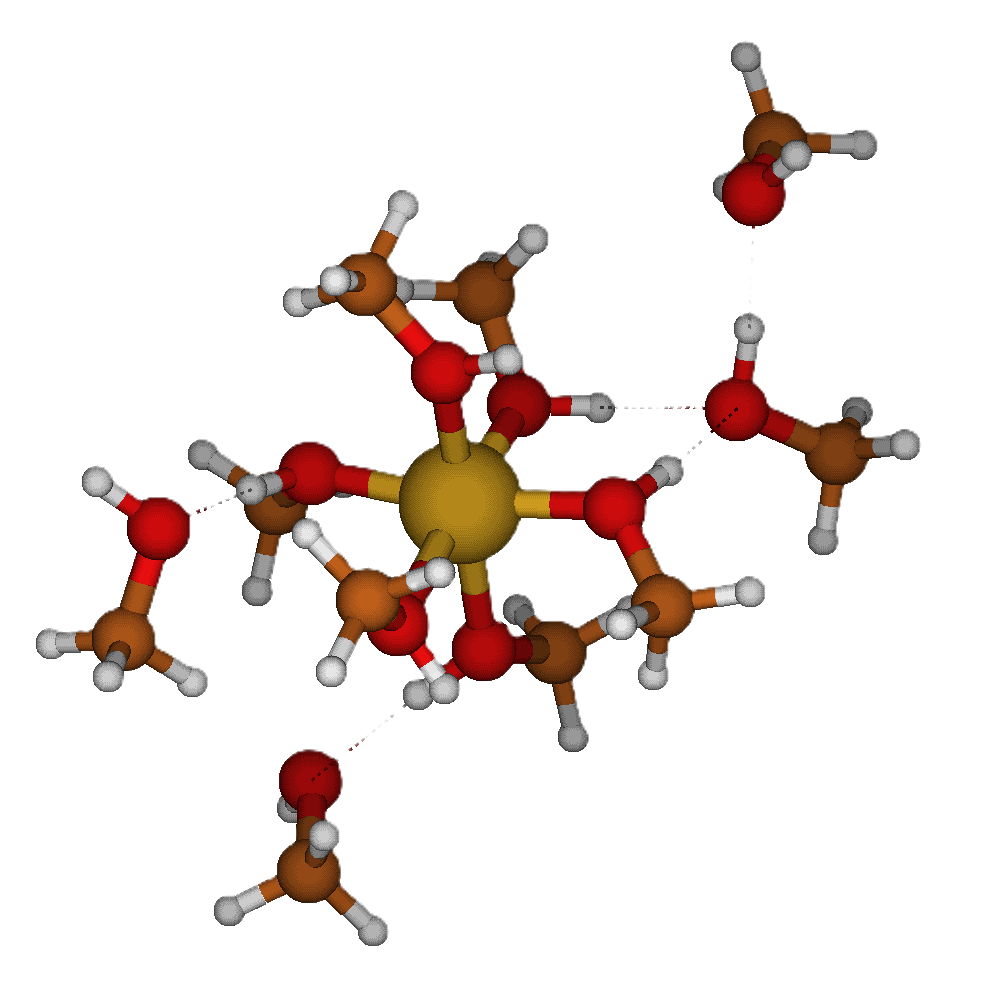
\includegraphics[width=\linewidth]{Imágenes/m_geometria_opt_n_10.png}
        \text{$n=10$}
    \end{minipage}\hfill
    \begin{minipage}[b]{0.3\textwidth}
        \centering
        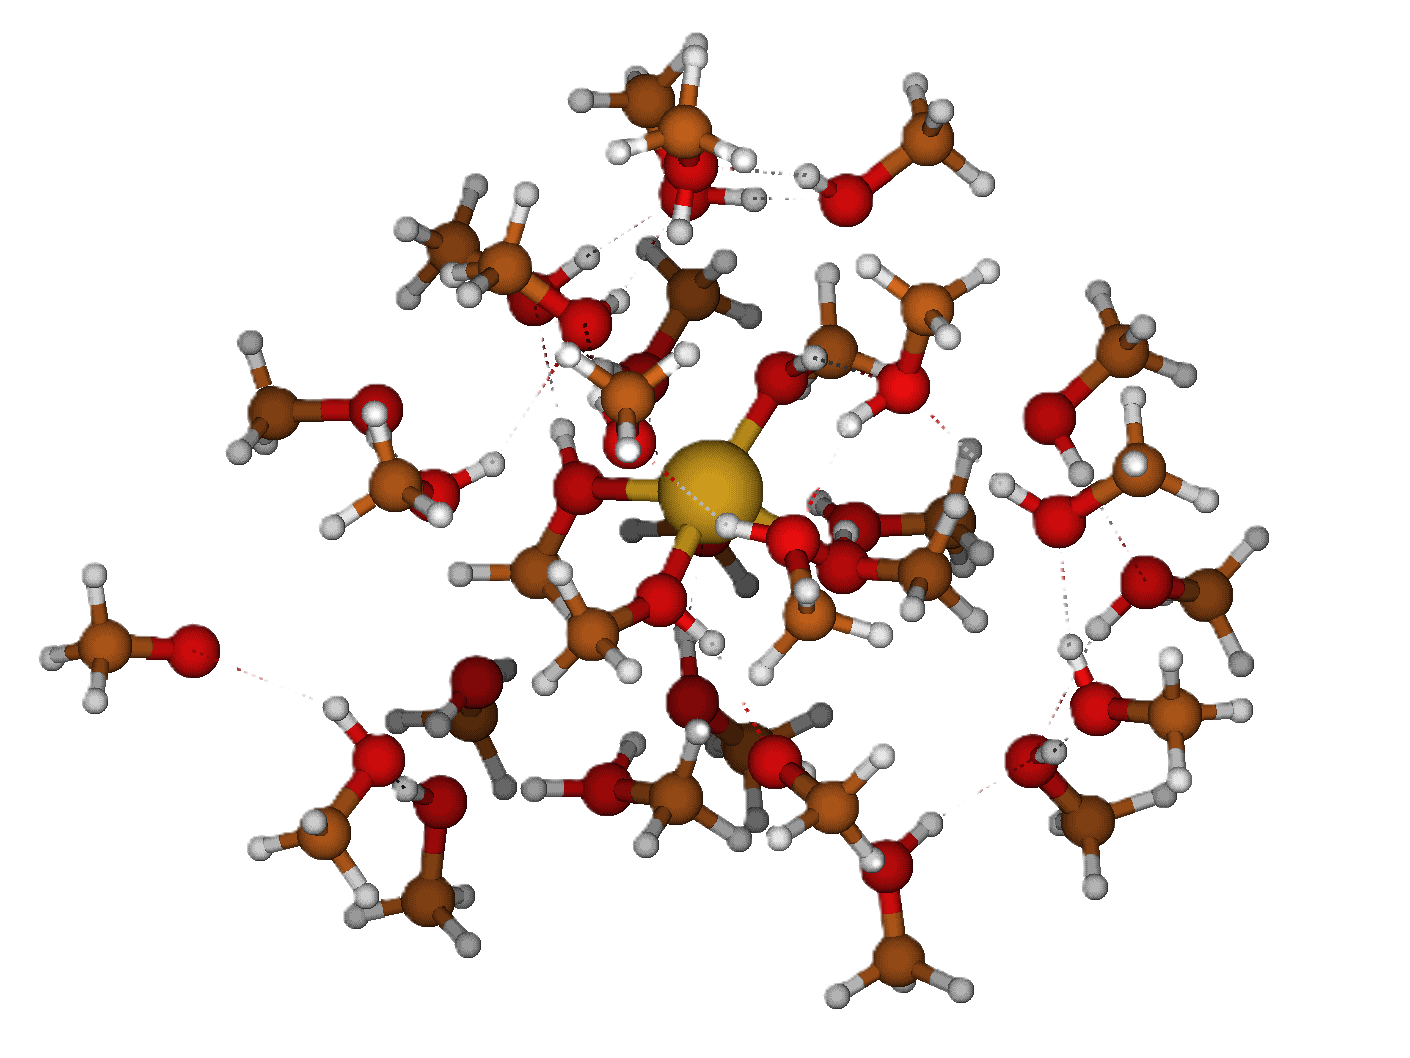
\includegraphics[width=\linewidth]{Imágenes/m_geometria_opt_n_30.png}
        \text{$n=30$}
    \end{minipage}\hfill
    \begin{minipage}[b]{0.3\textwidth}
        \centering
        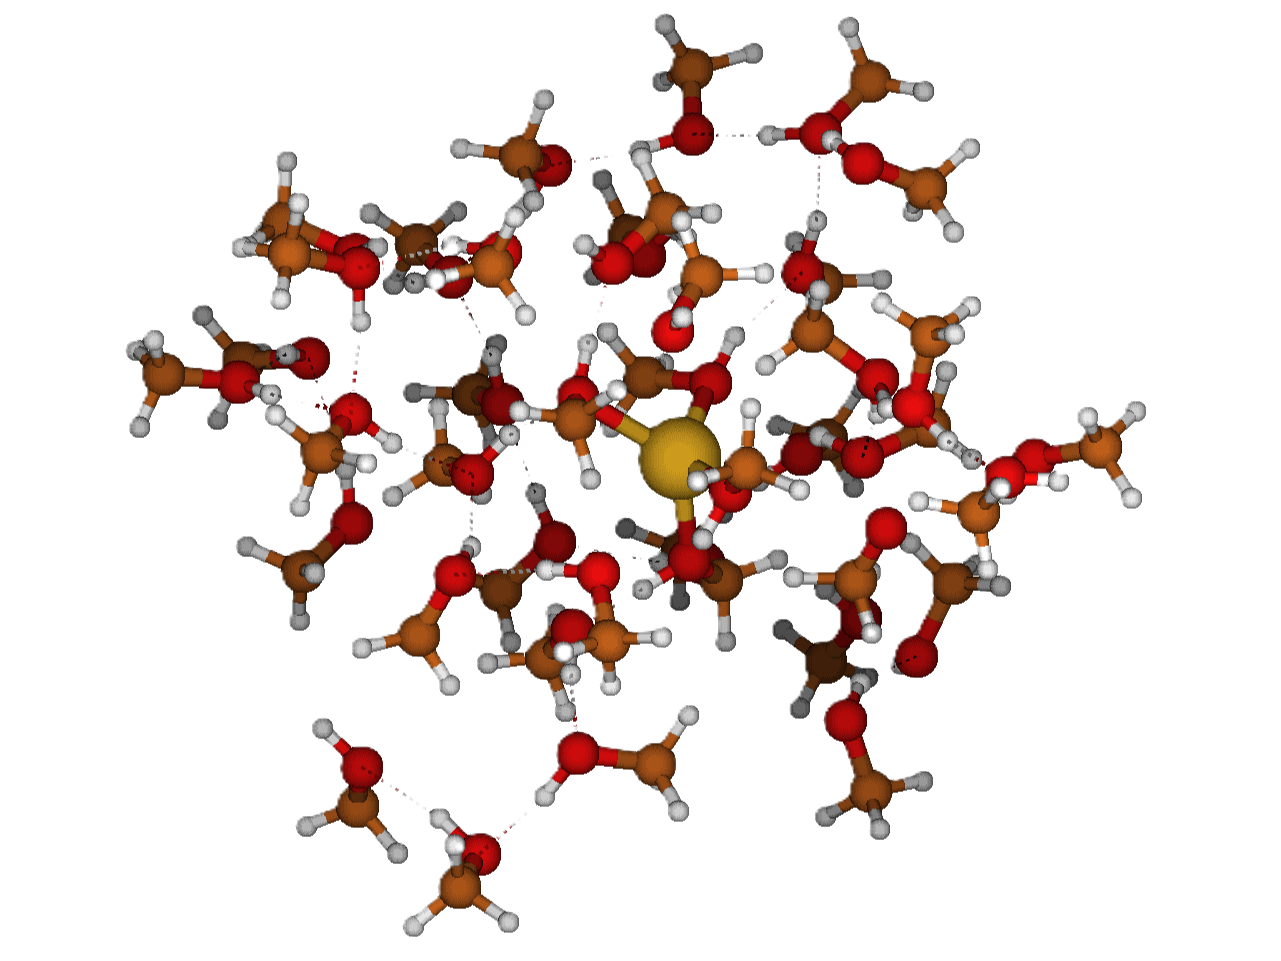
\includegraphics[width=\linewidth]{Imágenes/m_geometria_opt_n_40.png}
        \text{$n=40$}
    \end{minipage}
    \caption[Geometrías optimizadas con M06-2X/6-31G* \ce{[Cu(CH3OH)_{n}]^{2+}}]{Geometrías optimizadas para los cúmulos \ce{[Cu(CH3OH)_{n}]^{2+}} con $n = 1-10, 30, 40$ en el nivel de teoría M06-2X/6-31G*.}
    \label{fig:geo_opt_cumulos_m}
\end{figure}

\subsection{Selección del conjunto base}

Las simulaciones de BOMD tienen un costo computacional muy elevado, por ello resulta indispensable seleccionar un nivel de teoría que ofrezca un equilibrio óptimo entre la precisión y tiempo de cómputo requerido. Se ha documentado que el uso de conjuntos base extensos y con múltiples funciones difusas, como los de la serie aug-cc-pVDZ, hace que este tipo de simulaciones ab initio resulten impracticables cuando el ion interactúa con múltiples moléculas de solvente \cite{LeonPimentel2019}. Por el contrario, la familia de bases de Pople de tamaño moderado ha demostrado ser exitosa para modelar la solvatación de dicationes análogos en simulaciones BOMD \cite{CILP-2021-01, CILP-2023-01, CILP-2018-01, CILP-2018-02}. Para este fin, se evaluó el desempeño de las bases  6-31G*, 6-31+G* y 6-31+G** realizando para cada una de ellas la serie de optimizaciones descritas en la sección anterior e ilustradas en las figuras \ref{fig:geo_opt_cumulos} y \ref{fig:geo_opt_cumulos_m}. Adicionalmente, se optimizaron los cúmulos de 30 y 40 moléculas de solvente explícito para cada sistema. 

En esta fase de calibración, se analizó la coherencia en las tendencias energéticas, calculando la energía de enlace promedio por molécula de disolvente ($\Delta E / n$), magnitud que se define de manera general mediante la ecuación \ref{eq:energia_enlace}, donde $S$ representa la molécula de disolvente (agua o metanol):

\begin{equation}
    \frac{\Delta E}{n} = \frac{E\left(\ce{[Cu(S)_{n}]^{2+}}\right) - E(\ce{Cu^{2+}}) - n  E(S)}{n}\label{eq:energia_enlace}
\end{equation}

\begin{figure}[!t]
    \centering

    % --- Fila 1 ---
    \begin{minipage}[b]{0.48\textwidth}
        \centering
        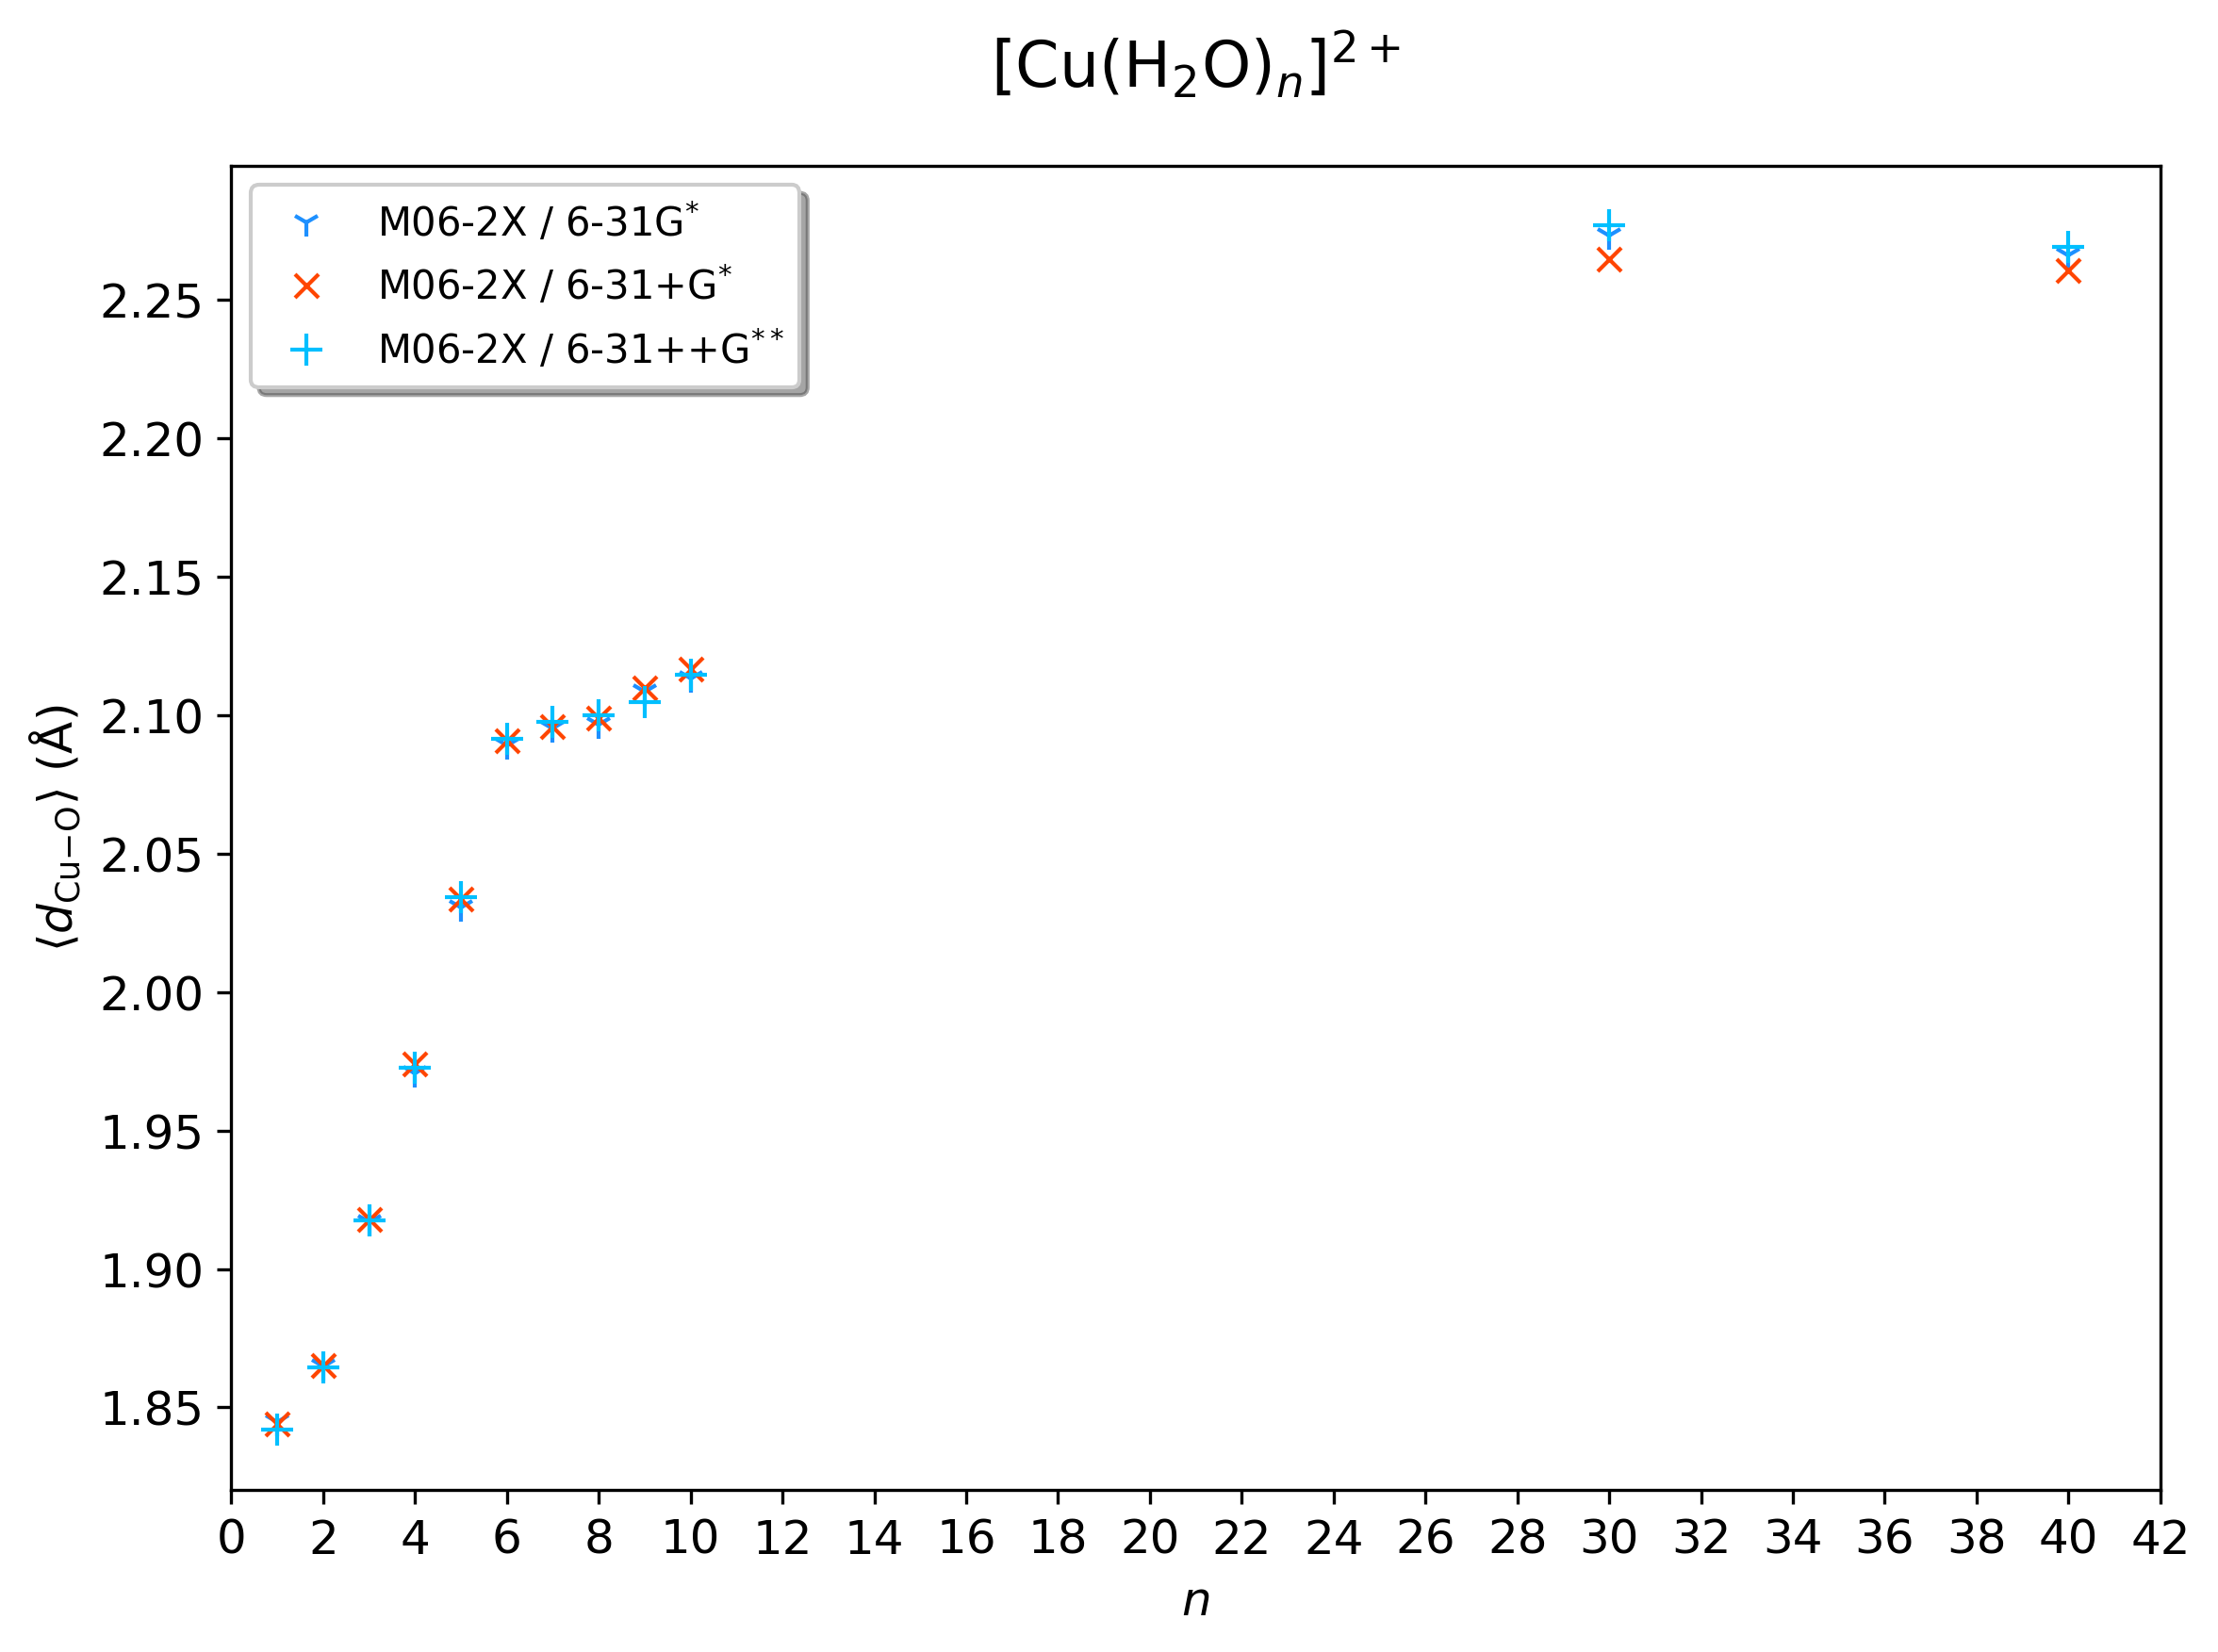
\includegraphics[width=\linewidth]{Imágenes/bases_agua_distancia.png}
    \end{minipage}
    \hfill
    \begin{minipage}[b]{0.48\textwidth}
        \centering
        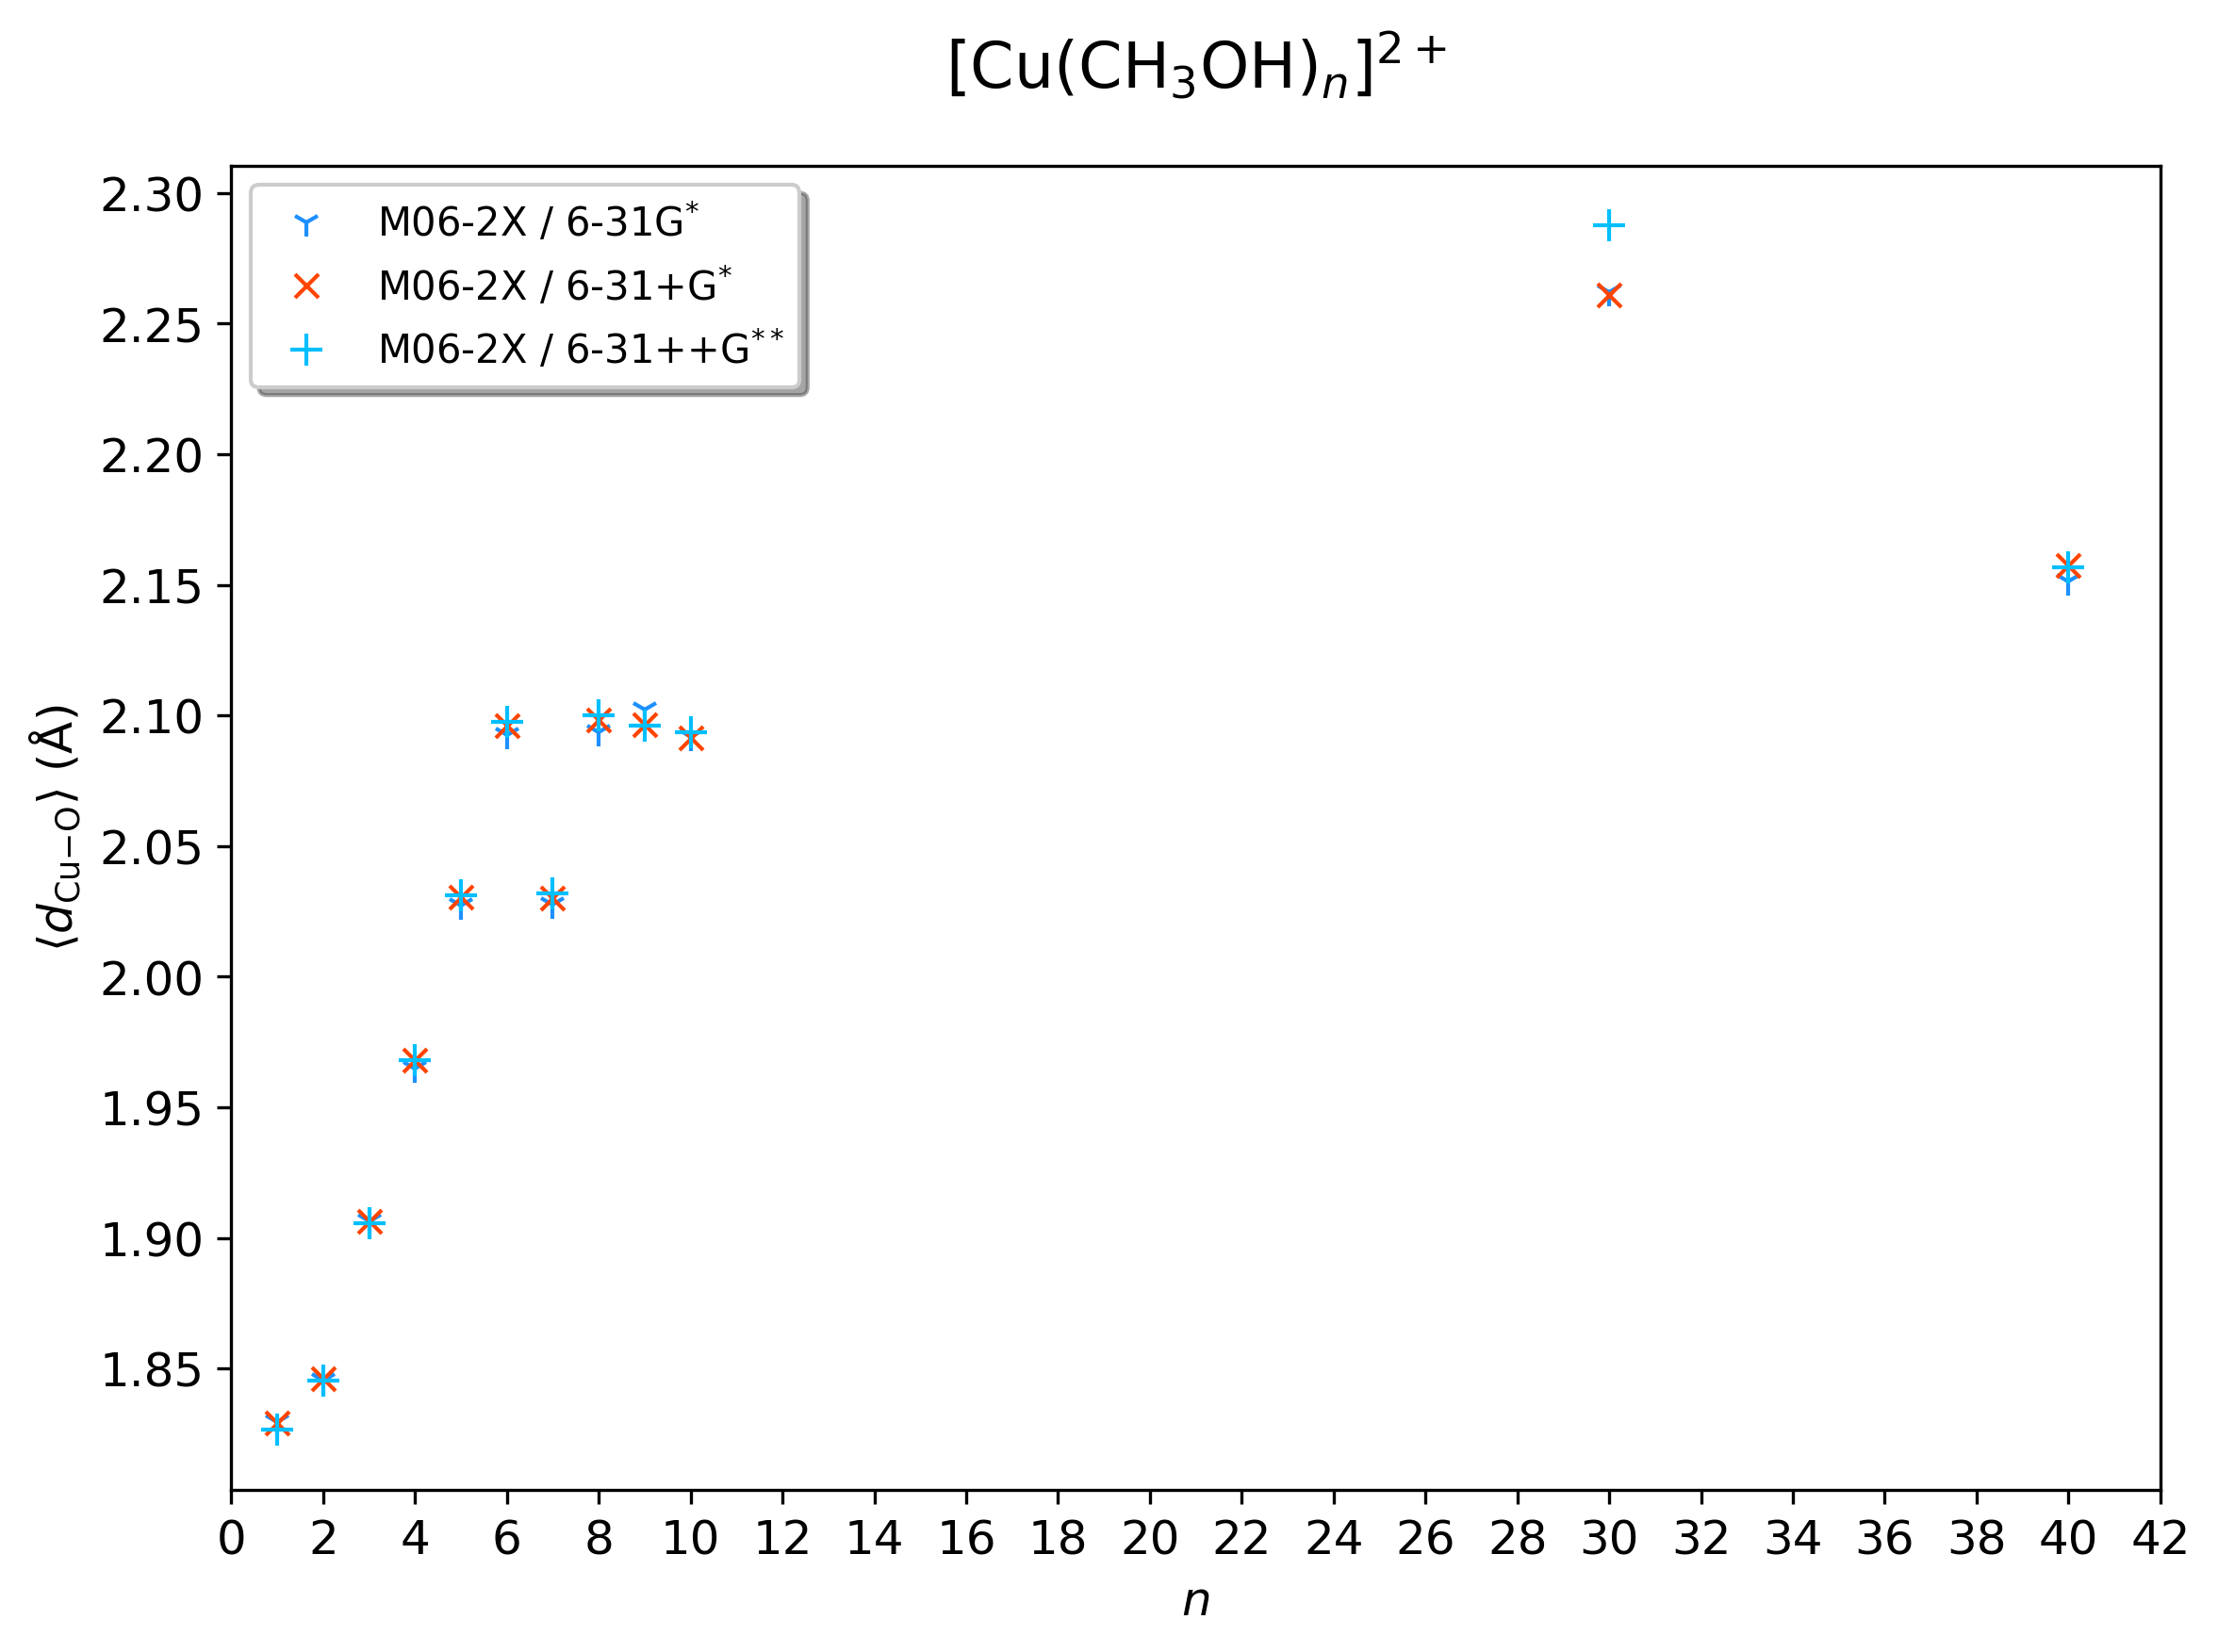
\includegraphics[width=\linewidth]{Imágenes/bases_metanol_distancia.png}
    \end{minipage}

    \vspace{0.4cm}

    % --- Fila 2 ---
    \begin{minipage}[b]{0.48\textwidth}
        \centering
        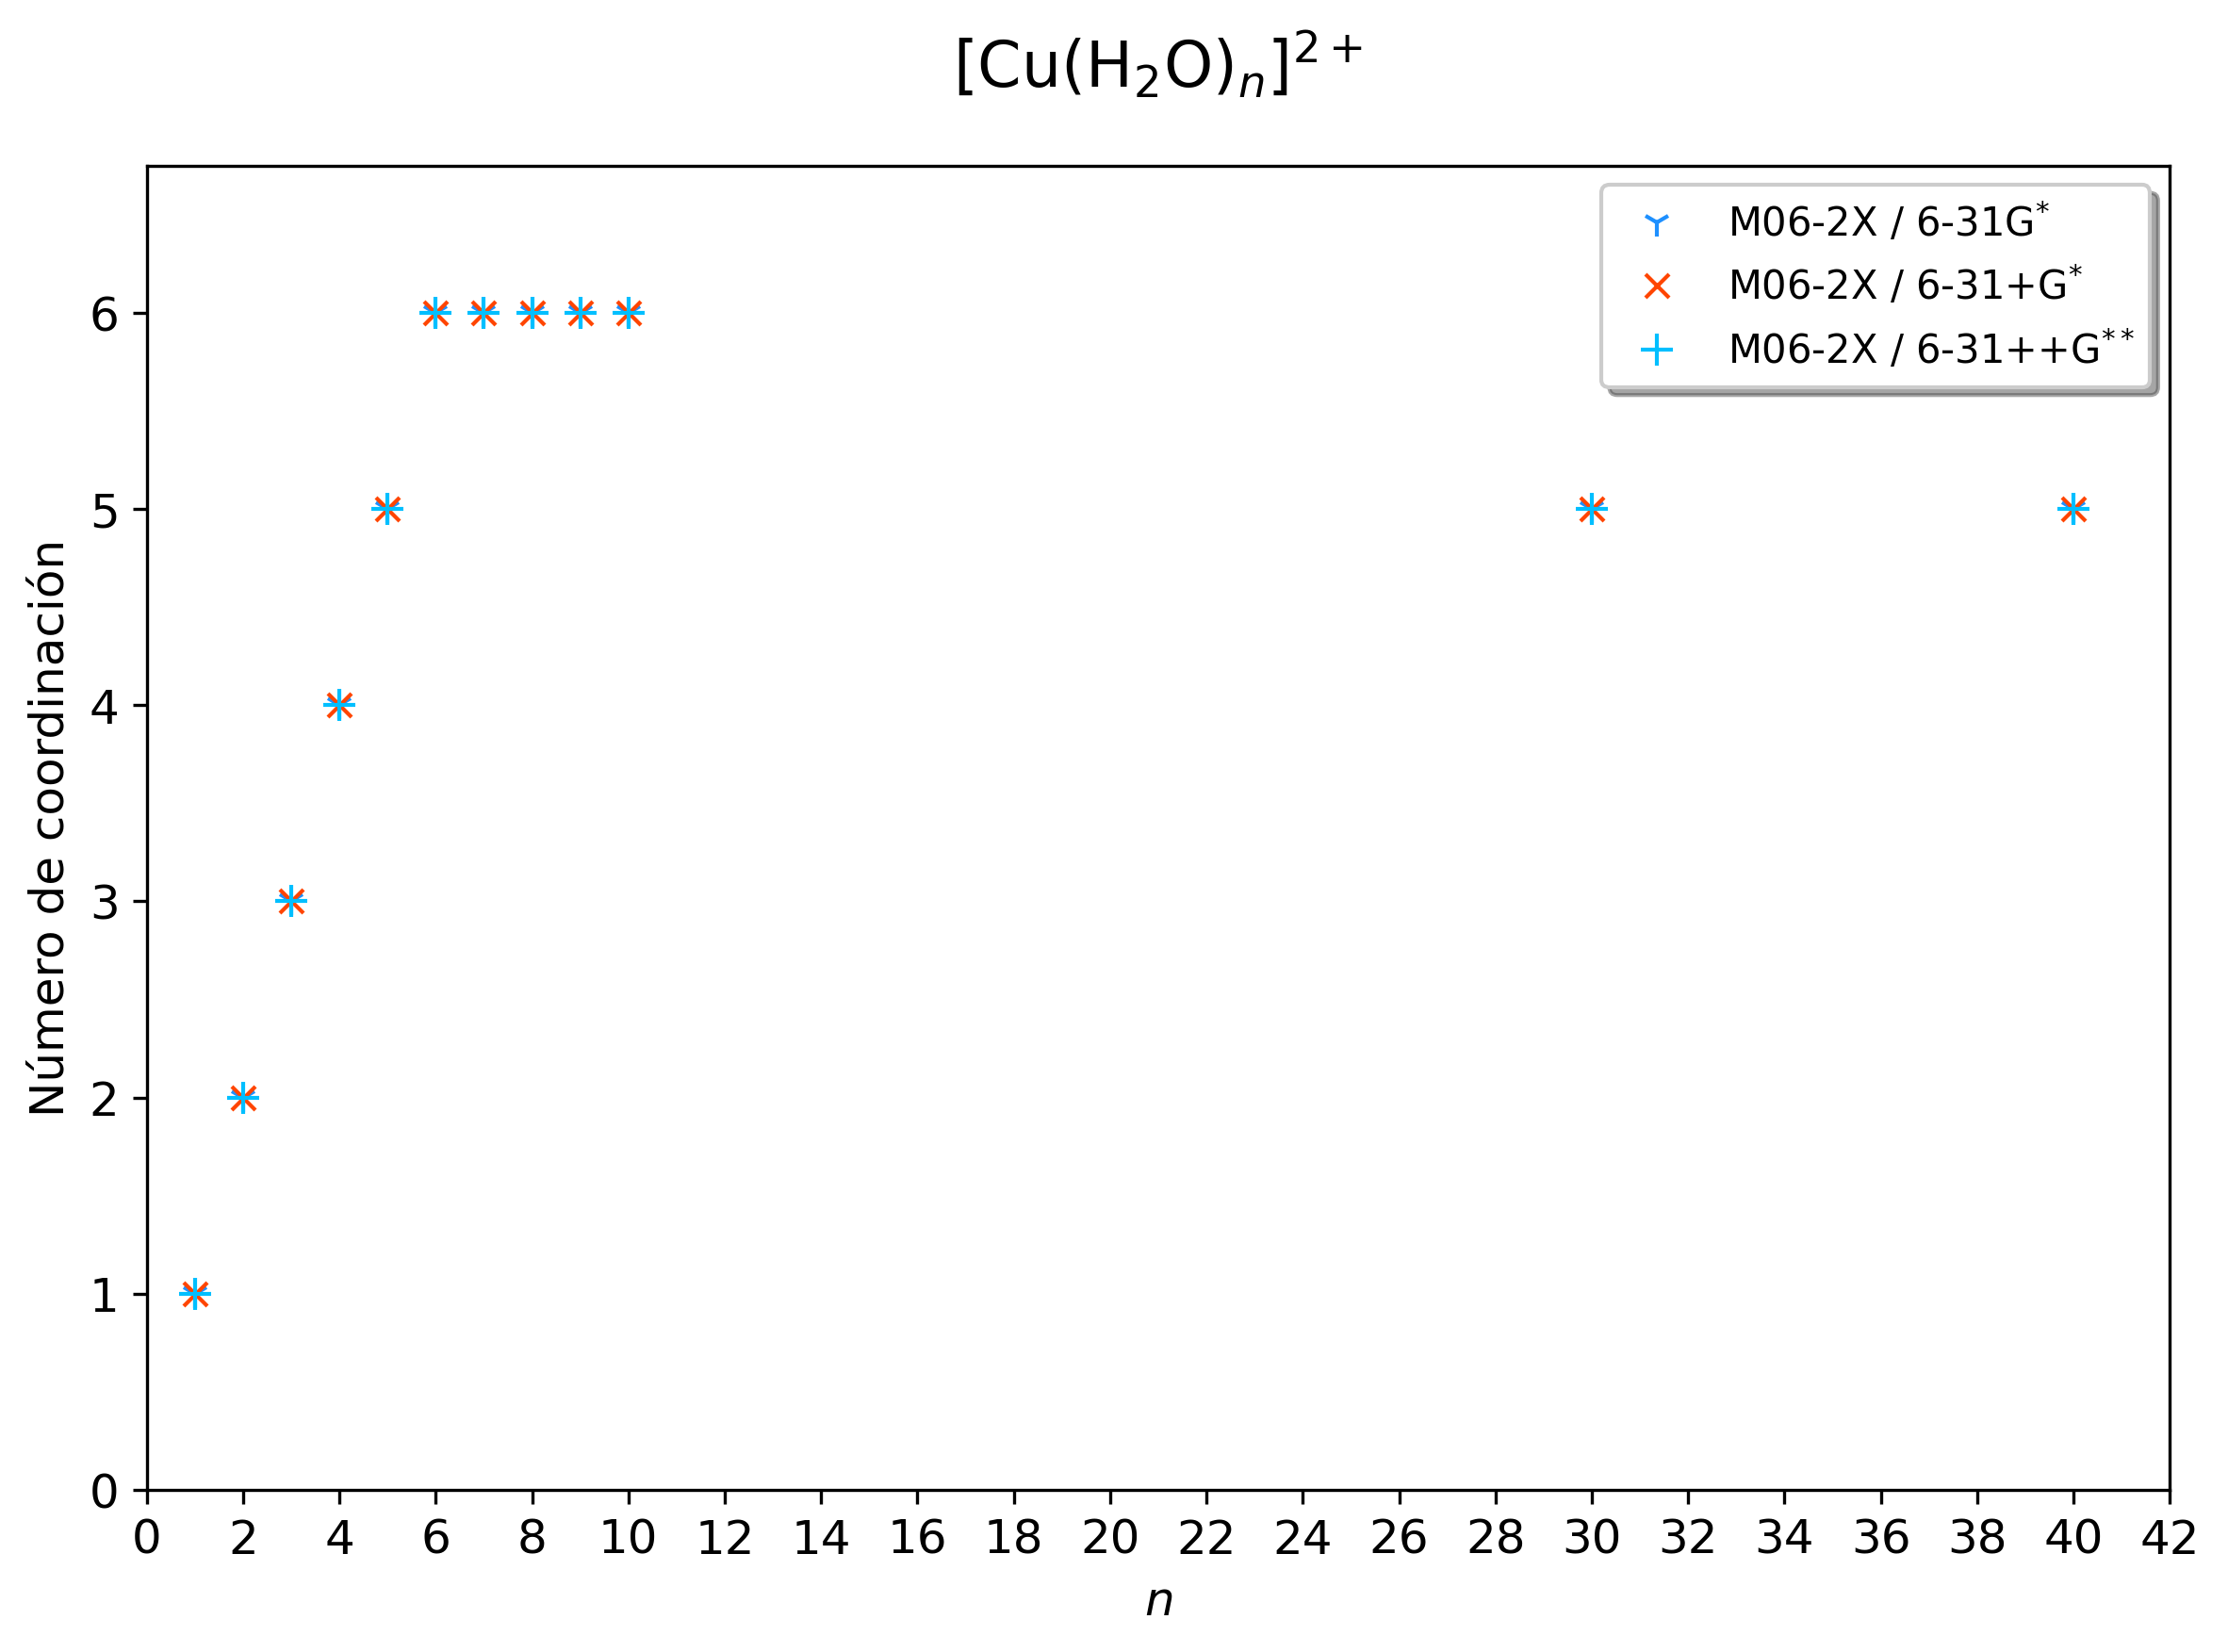
\includegraphics[width=\linewidth]{Imágenes/bases_agua_ncoord.png}
    \end{minipage}
    \hfill
    \begin{minipage}[b]{0.48\textwidth}
        \centering
        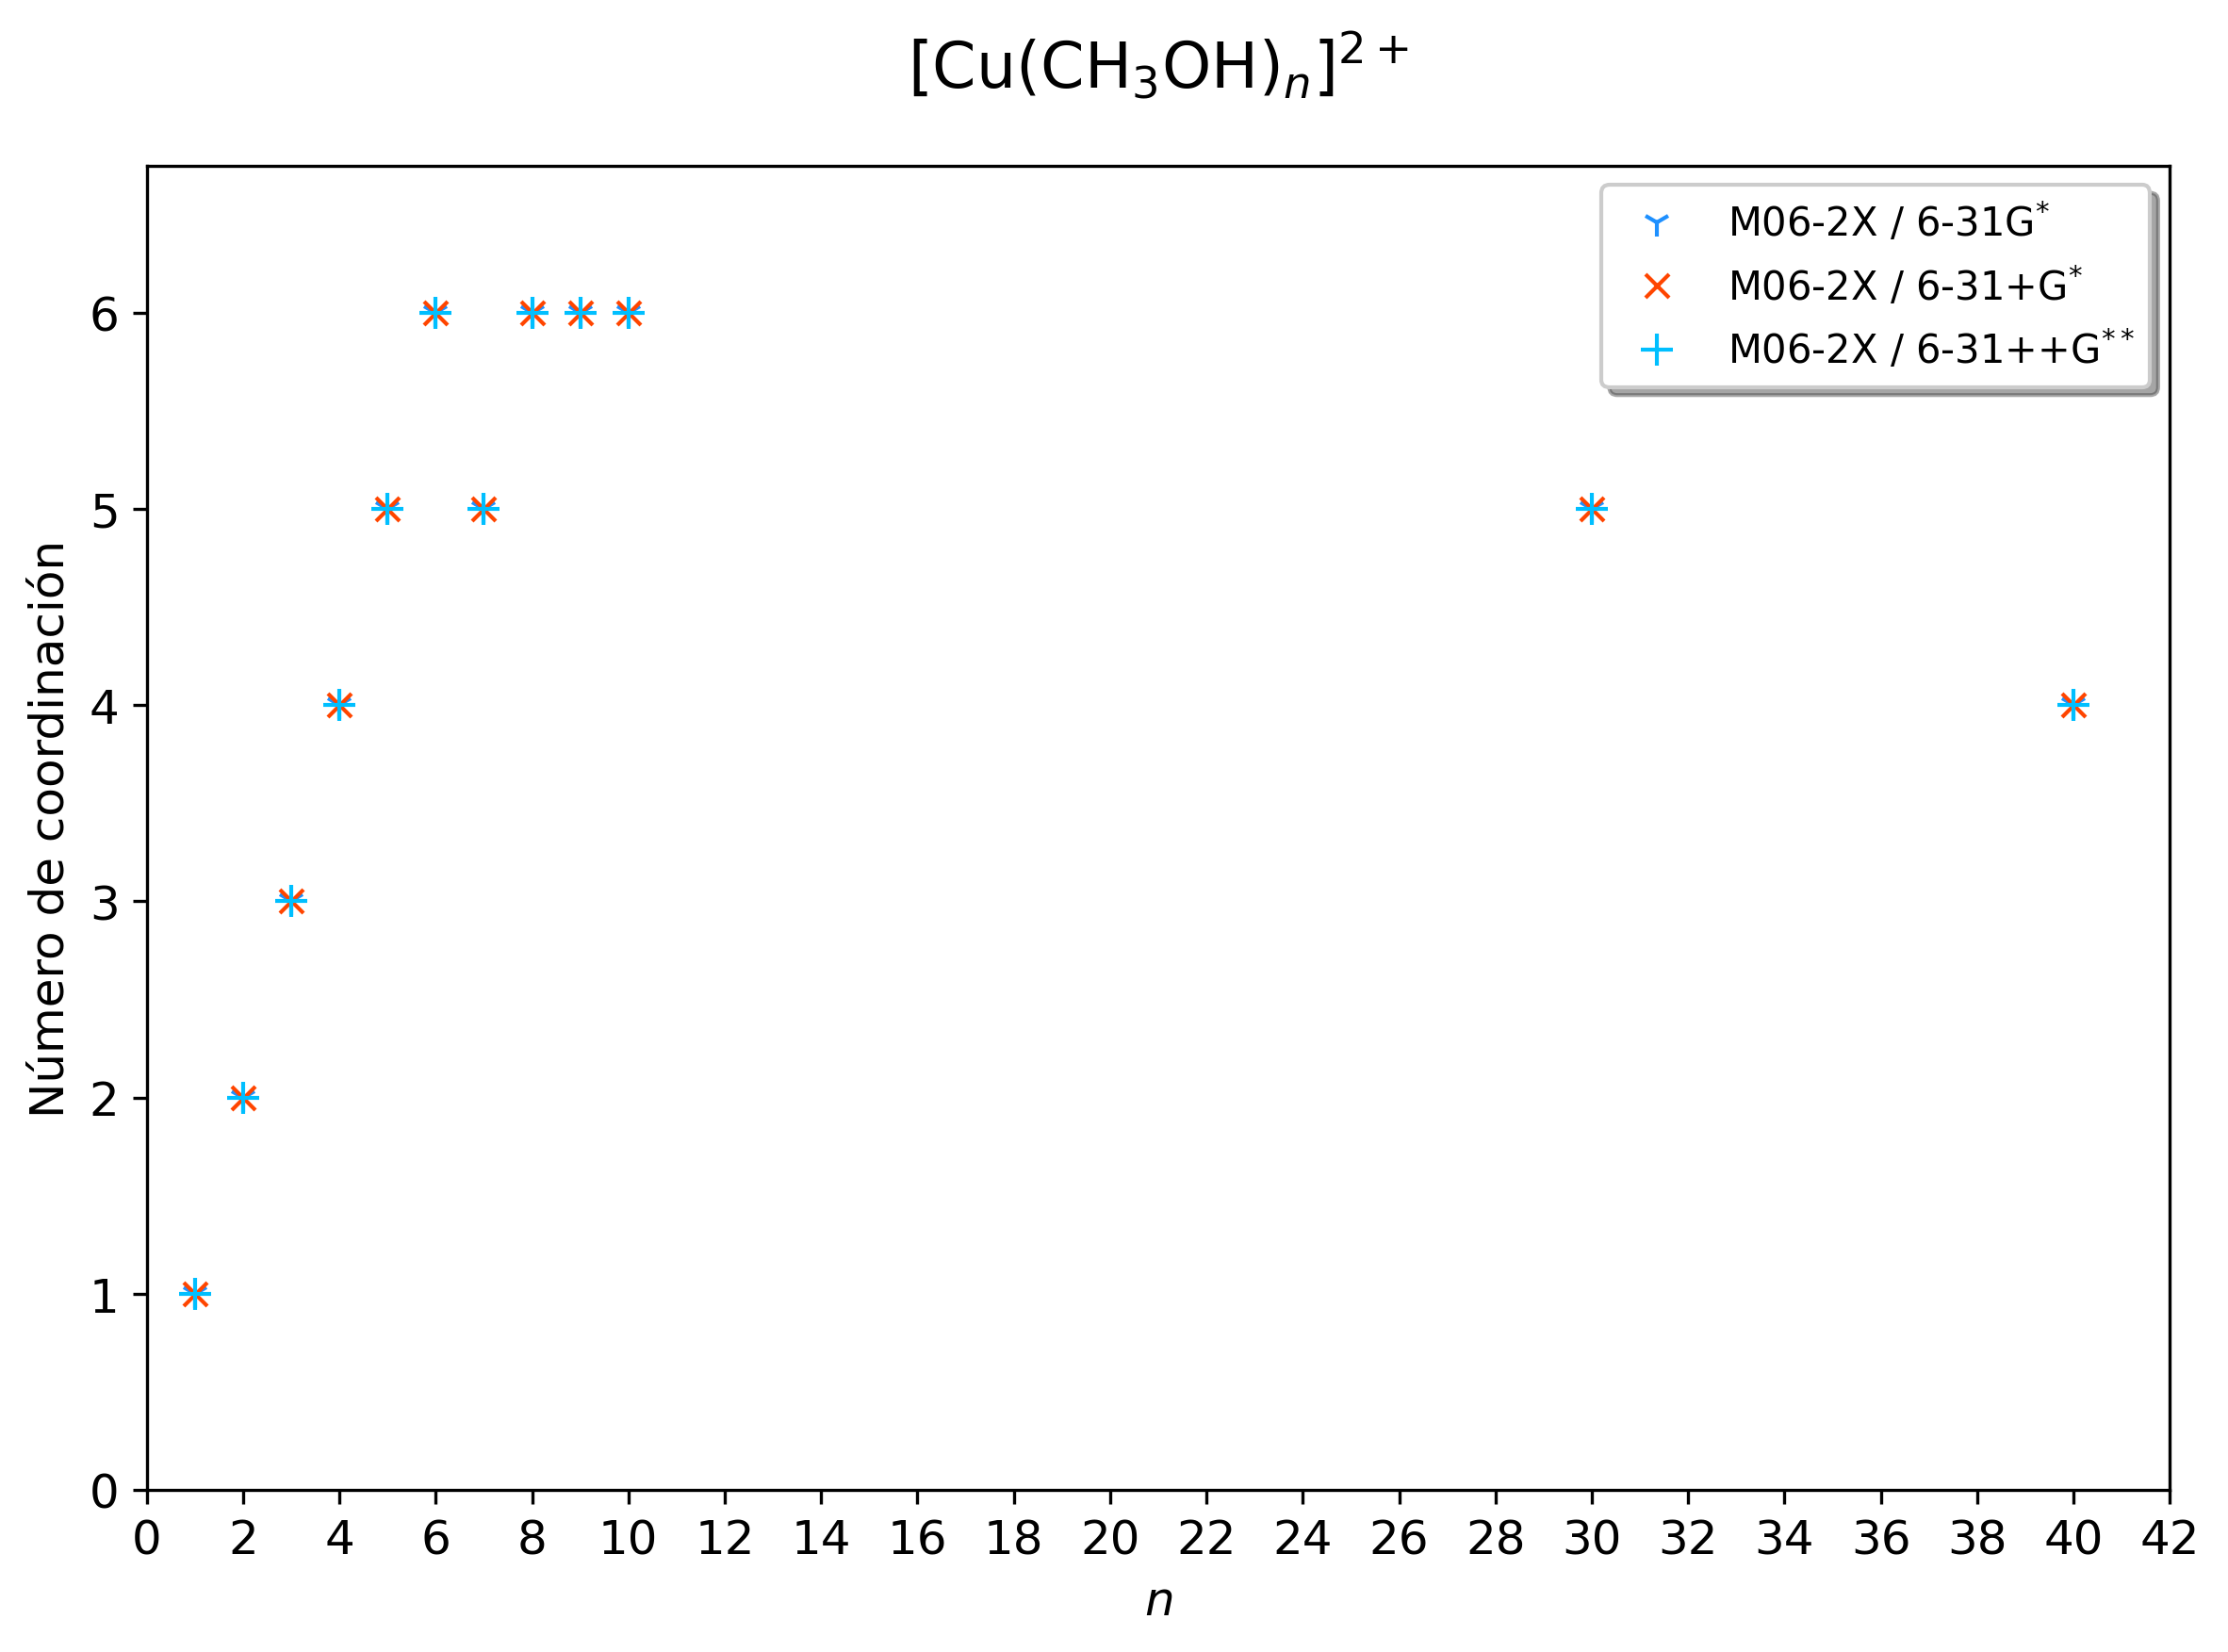
\includegraphics[width=\linewidth]{Imágenes/bases_metanol_ncoord.png}
    \end{minipage}

    \caption[Distancia Cu–O promedio y número de coordinación vs $n$ por conjunto base]{
        Distancia Cu–O promedio de la primera esfera de coordinación (fila superior) 
        y número de coordinación (fila inferior) en función del número de moléculas 
        de solvente $n$, calculados para los sistemas \ce{[Cu(H2O)_n]^{2+}} (izquierda) 
        y \ce{[Cu(CH3OH)_n]^{2+}} (derecha) con los conjuntos base 
        6-31G$^*$, 6-31+G$^*$ y 6-31++G$^{**}$. El radio de corte utilizado para definir la 
        primera esfera es $r = 2.833$~\AA{} para agua y 
        $r = 3.023$~\AA{} para metanol.
    }
    \label{fig:bases_estructural}
\end{figure}

\begin{figure}[p]
    \centering
    
    % Gráfica 1 (Agua)
    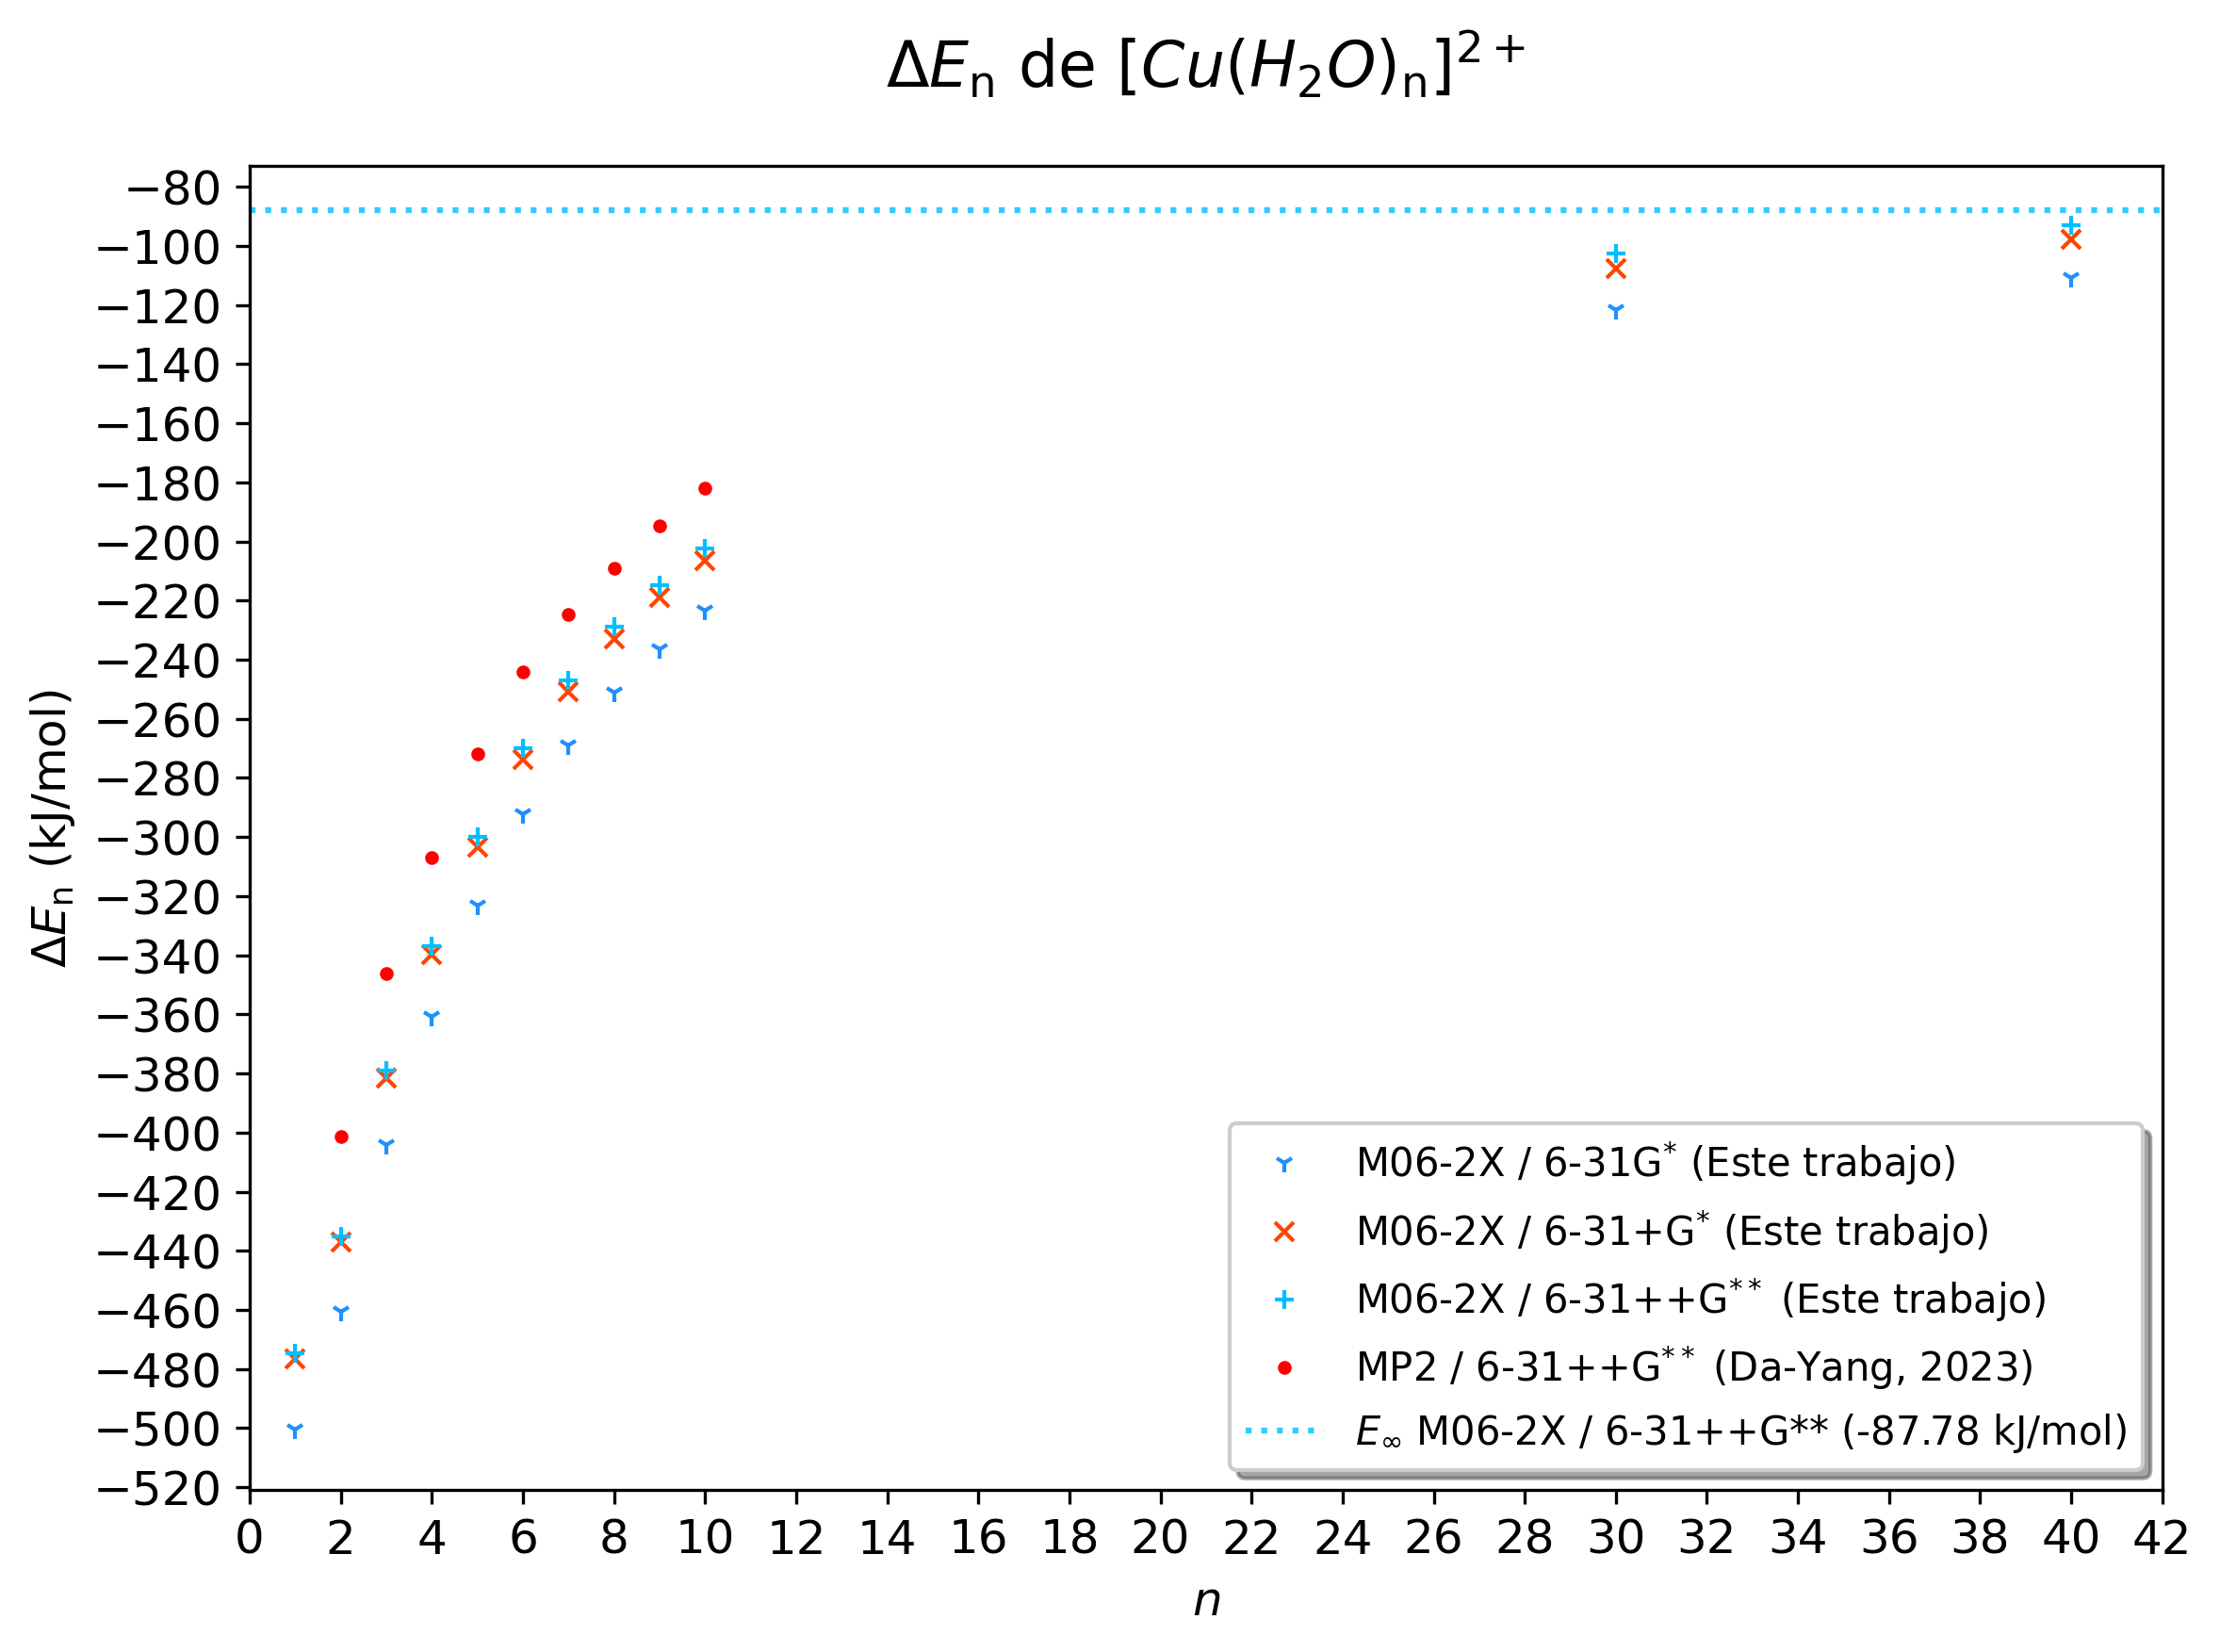
\includegraphics[width=0.85\textwidth]{Imágenes/bases_agua.png}
    
    % Un pequeño espacio vertical entre las gráficas
    \vspace{0.5cm} 
    
    % Gráfica 2 (Metanol)
    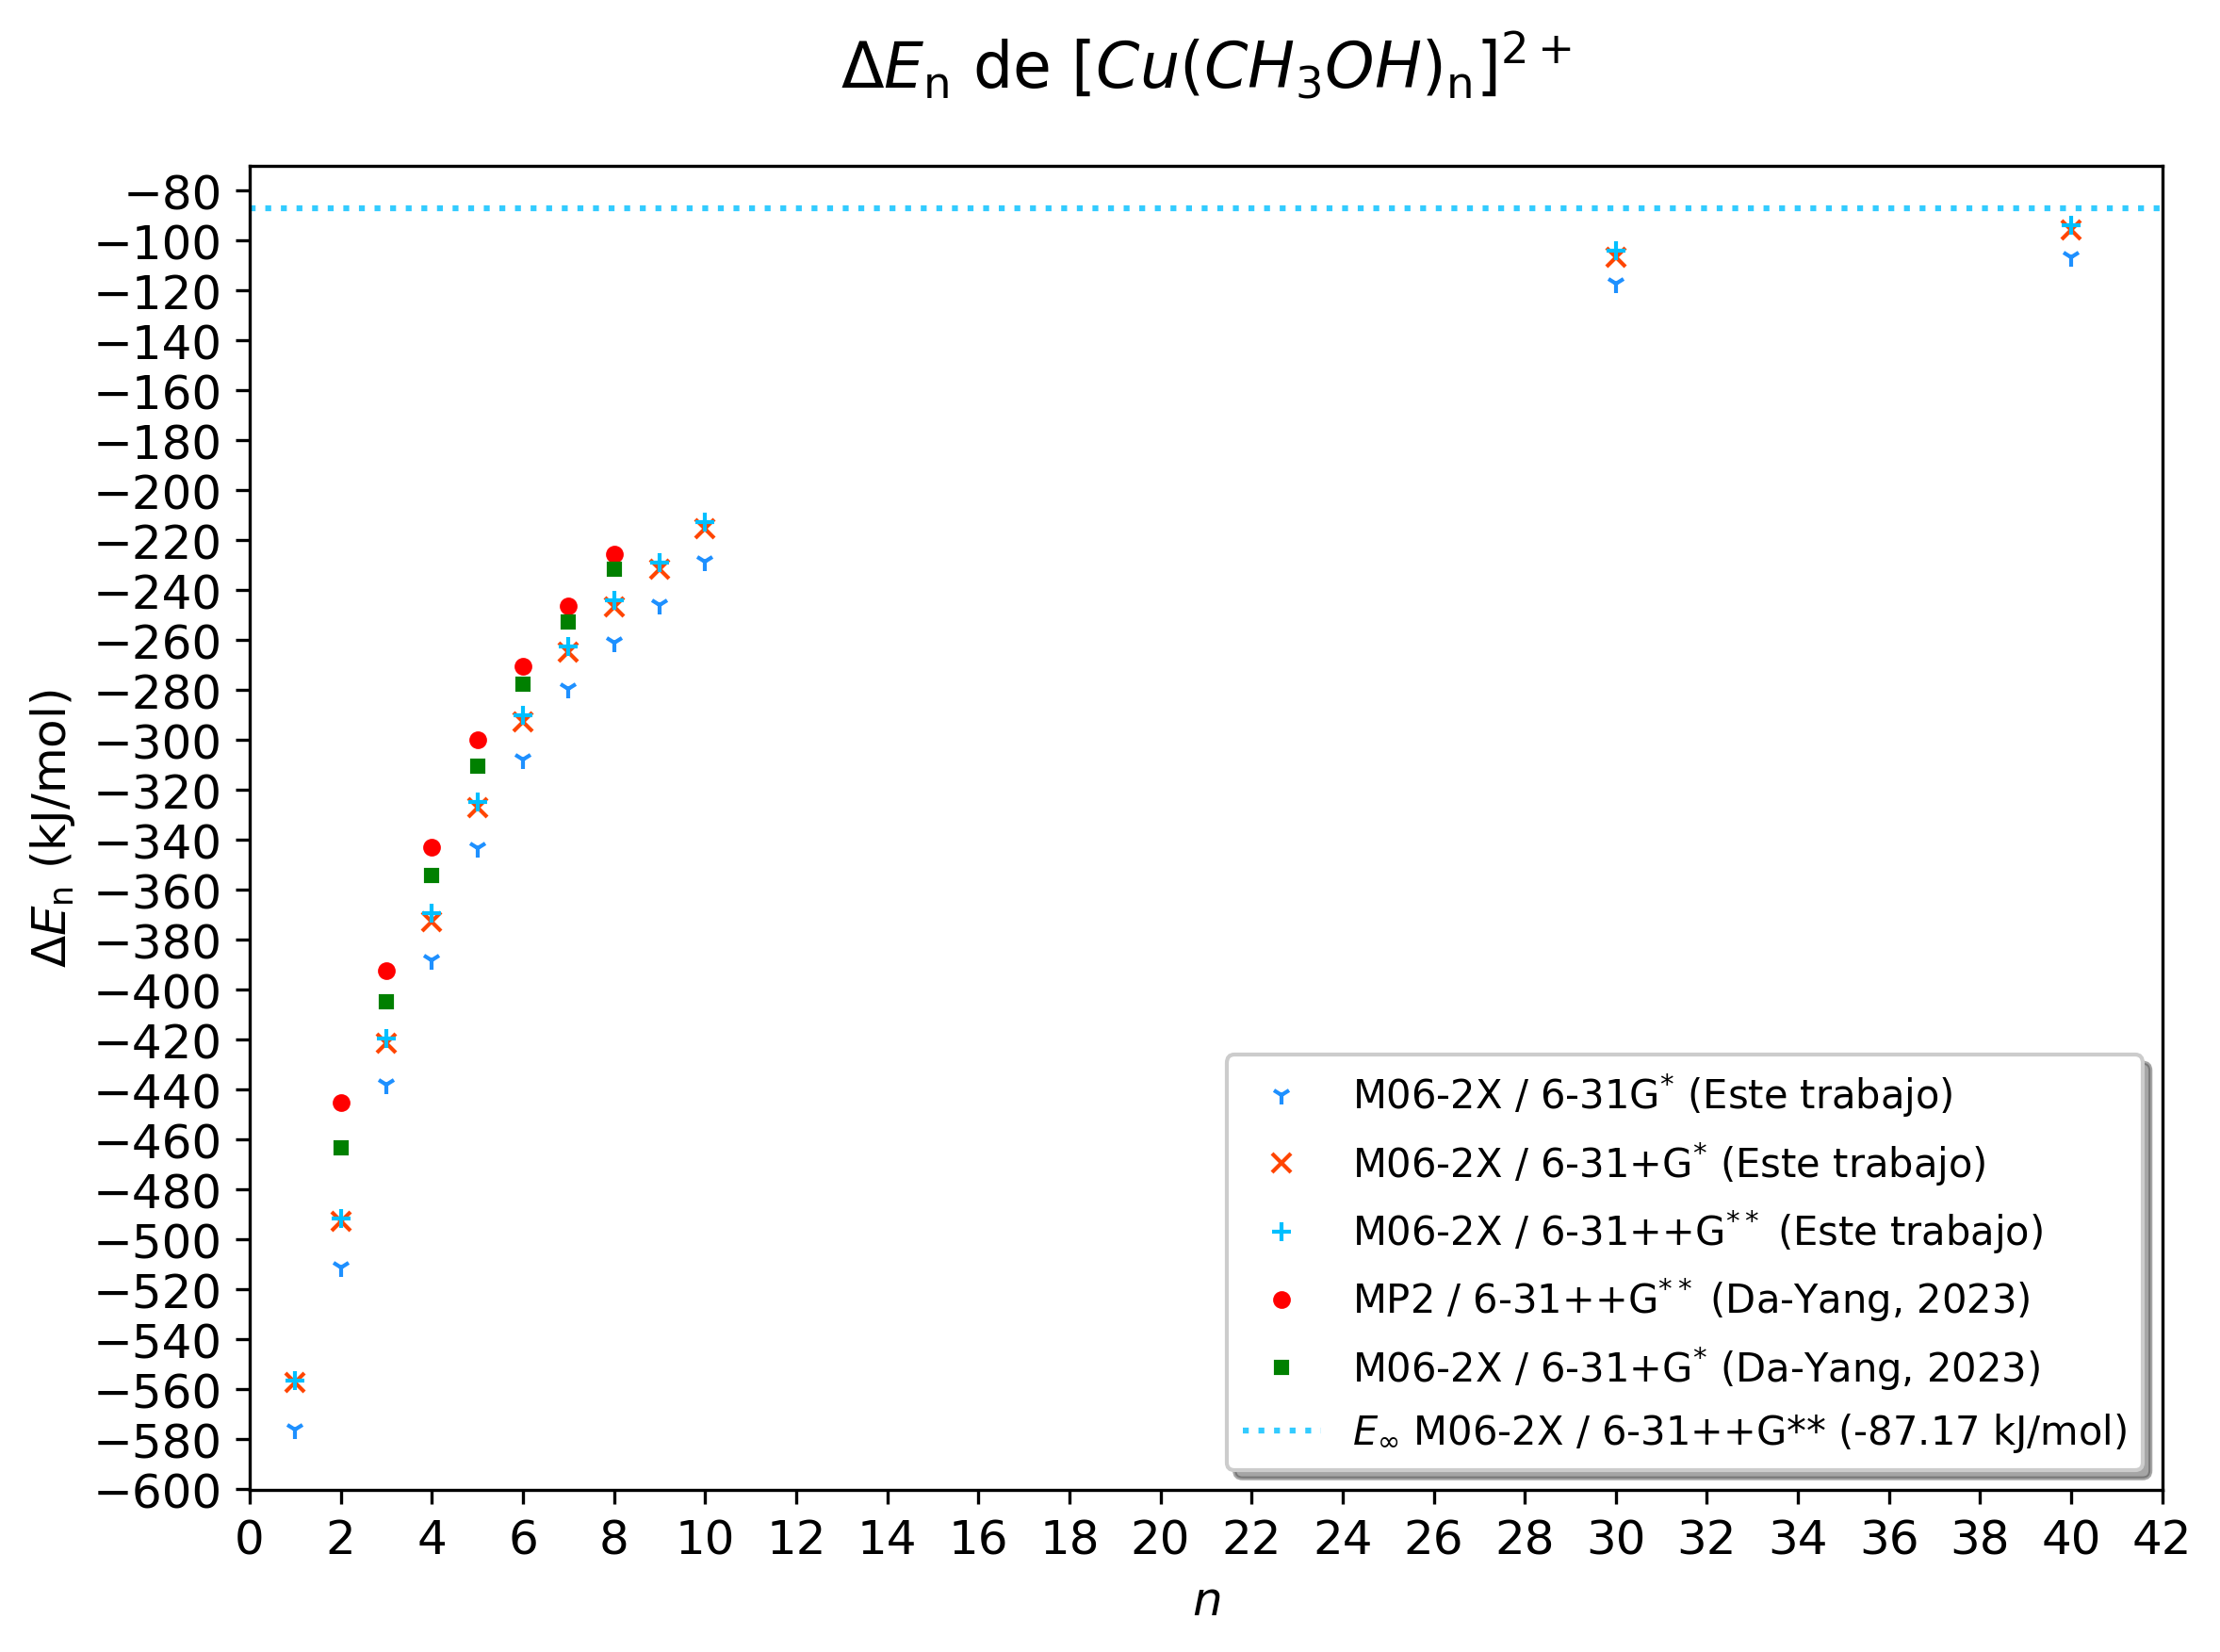
\includegraphics[width=0.85\textwidth]{Imágenes/bases_metanol.png}

    % --- LEYENDA ACTUALIZADA ---
    \caption[Energías de enlace por molécula de solvente \ce{[Cu(H2O)_{n}]^{2+}} \ce{[Cu(CH3OH)_{n}]^{2+}}]{Energías de enlace por molécula de solvente calculada para las estructuras de solvatación óptimas de \ce{[Cu(H2O)_{n}]^{2+}} (arriba) y \ce{[Cu(CH3OH)_{n}]^{2+}} (abajo), con $n = 1,\ 2,\ \ldots,\ 10,\ 30,\ 40$, mediante cálculos de optimización con los niveles de teoría 6-31G$^\ast$, 6-31+G$^\ast$ y 6-31++G$^{\ast\ast}$. Resultados obtenidos con MP2 \cite{Me-2022-01} y validación de M06-2X respecto a MP2 \cite{Me-2023-01}. Las energías reportadas para $n=30$ y $n=40$ no corresponden a mínimos globales pues el cálculo para cúmulos de este tamaño conlleva una complejidad que excede el alcance de la presente tesis.}
    \label{fig:bases}
\end{figure}

En la Figura \ref{fig:bases}, se observa que el conjunto base 6-31G* presenta una ligera discrepancia energética respecto a las bases 6-31+G* y 6-31++G**. No obstante, estas dos últimas describen el sistema de manera prácticamente idéntica, lo que sugiere que la adición de funciones difusas en los átomos de hidrógeno no aporta una corrección significativa en comparación con la inclusión de estas funciones únicamente en el \ce{Cu^{2+}}. 

La selección del conjunto base para las simulaciones BOMD se fundamenta en dos criterios. En primer lugar, la similar descripción estructural de los óptimos: la Figura \ref{fig:bases_estructural} muestra la distancia Cu--O promedio en la primera esfera de coordinación y el número de coordinación en función de $n$ para los tres conjuntos base. Ambas magnitudes convergen al mismo óptimo estructural con distancias y números de coordinación prácticamente idénticos entre las tres bases, lo que corrobora su consistencia geométrica. En segundo lugar, la concordancia en la tendencia cualitativa de la energía de enlace: si bien la base 6-31G* produce energías de enlace ligeramente distintas a las de las bases más extendidas, las curvas son paralelas entre sí, lo que indica que los tres conjuntos base describen paisajes energéticos equivalentes (véase Figura \ref{fig:bases}). Con base en estos criterios, se seleccionó el nivel de teoría M06-2X/6-31G* como el que ofrece el mejor equilibrio entre precisión y costo computacional para las simulaciones BOMD.

Un punto de discusión relevante es el límite asintótico de la energía de enlace por molécula de solvente ($n \to \infty$). Según Da-Yang et al \cite{Wa-2024-03}, para el sistema en agua a un nivel de alto nivel en fase gaseosa (CCSD(T)//MP2), este límite converge a $-179.9 \pm 1.7$ kJ/mol. En el caso del metanol en fase gaseosa (MP2), el límite reportado es de $-158.9$ kJ/mol \cite{Me-2022-01}. Sin embargo, al incorporar efectos de solvente implícito mediante el modelo IEF-PCM, dichos autores reportan que el límite se reduce notablemente a valores entre $-105.9$ y $-88.6$ kJ/mol. En el presente trabajo, se realizó una extrapolación de la energía de enlace utilizando el modelo de decaimiento exponencial $E(n) = E_\infty + A e^{-bn}$, ajustado con los datos de los cúmulos más grandes ($n=10, 30, 40$). Los límites obtenidos para el nivel M06-2X/6-31++G** son $E_\infty = -87.78$ kJ/mol para el caso de agua y $E_\infty = -87.17$ kJ/mol para el sistema de metanol. Estos valores se sitúan en la zona de los resultados de Da-Yang cuando estos últimos incluyen el medio continuo (IEF-PCM). Es importante señalar que si se aplica el modelo de ajuste de Da-Yang a nuestros primeros 10 datos, se obtiene la misma tendencia energética; no obstante, la extrapolación basada en los primeros 10 puntos no necesariamente describe con exactitud la fenomenología del enlace en cúmulos de gran tamaño. Cabe precisar que las energías reportadas para $n=30$ y $n=40$ corresponden a mínimos locales pues la búsqueda del mínimo global absoluto para cúmulos de este tamaño conlleva una complejidad combinatoria que queda fuera del alcance de este trabajo.

%%%%%%%%
\section{Simulaciones}

Para evaluar la viabilidad técnica y estimar los tiempos de ejecución necesarios para alcanzar trayectorias representativas de al menos 20 picosegundos, se iniciaron simulaciones de dinámica molecular con los cúmulos optimizados de 30 y 40 moléculas para ambos sistemas usando el módulo \texttt{orca\_md} del software ORCA v6.1 \cite{orca, orca6.1}, estableciendo un periodo de termalización inicial de 6,000 pasos. De acuerdo con la literatura \cite{Me-2023-01}, la energía promedio de enlace por molécula de solvente alcanza la saturación asintótica para sistemas con $n \geq 35$. Tomando en consideración este antecedente, y dado que la diferencia en el costo computacional entre los sistemas de 30 y 40 moléculas no resultó prohibitiva, se seleccionó el cúmulo con $n = 40$ para llevar a cabo las simulaciones definitivas.

Las simulaciones se ejecutaron manteniendo el nivel de teoría M06-2X/6-31G* con corrección de dispersión D3(0), empleando el pseudopotencial y la base extendida para el ion \ce{Cu^{2+}} detallados en la sección \ref{section-optimización}. El flujo general de cálculo, que acopla la integración de las ecuaciones de movimiento nuclear con la resolución del campo autoconsistente SCF electrónico en cada paso de tiempo, se ilustra en la Figura \ref{fig:metodologia}. Los parámetros termodinámicos e integradores establecidos para todas las dinámicas se resumen en la tabla \ref{tab:md_params}.

\begin{table}[htbp]
    \centering
    \caption{Parámetros termodinámicos e integradores empleados para las simulaciones de Dinámica Molecular.}
    \label{tab:md_params}
    \begin{tabular}{ll}
        \hline
        \textbf{Parámetro} & \textbf{Valor} \\ \hline
        Ensamble & NVT (Canónico) \\
        Temperatura objetivo ($T$) & 300 K \\
        Asignación de velocidad inicial & Maxwell-Boltzmann (a 300 K) \\
        Termostato & Cadena de Nosé-Hoover (NHC) \\
        \quad - Longitud de la cadena & 4 \\
        \quad - Integrador & Yoshida-7 \\
        Paso de tiempo ($\Delta t$) & 0.5 fs \\
        Tiempo total de producción & 30 ps \\
        Pasos totales de producción & 60,000 \\
        Frecuencia de muestreo & 1 paso (0.5 fs) \\ \hline
    \end{tabular}
\end{table}

\begin{figure}[p] 
    \centering
    \caption[Diagrama general de cálculo. Bucles SCF y DM]{Diagrama general de cálculo. Los dos principales bucles son los referentes al método de campo autoconsistente (SCF) y al principal de la dinámica molecular.}
    \label{fig:metodologia}
    \vspace{0.5cm}
    
    \rotatebox{90}{
        \begin{tikzpicture}[
        scale=0.4, transform shape,
        font=\large\sffamily,
        node distance = 8mm and 15mm, 
        block/.style = {rectangle, draw, text centered, rounded corners,
                        minimum height=2.2cm, align=center},
        diamond_dec/.style = {diamond, draw, text centered, aspect=2,
                              inner sep=1pt, text width=2.5cm},
        line/.style = {-{Stealth[length=2.5mm]}}
        ]

        % --- Fila Superior ---
        \node[block] (cond) {\textbf{Inicialización}  \\ $\mathbf{R}^{N}(t=0)$};
        \node[block, right=of cond] (opt_structure) {\textbf{Optimizar estructura} \\ {\text{Minimizar energía}} \\ $\mathbf{R}^{N}_{min}(0)$};
        \node[block, right=of opt_structure](init_vel) {\textbf{Velocidades} \\ \textbf{iniciales} \\$\mathbf{V}^{N}(t=0)$};
        \node[block, right=of init_vel] (t_step) { \textbf{Bucle SCF} \\ $t^{(n)}$};

        % --- Fila Intermedia (Bucle SCF) ---
        % CORRECCIÓN: \rho(\mathbf{r}) en lugar de \rho(r)
        \node[block, right=3cm of t_step] (propose_rho){ \textbf{Proponer} \\$\rho^{(n)}(\mathbf{r})$};
        
        % CORRECCIÓN: \hat{H} y \mathbf{r} implicito en nabla
        \node[block, below=2.3cm of propose_rho] (build_h) {\textbf{Construir hamiltoniano} \\ $\hat{H}^{(n)}_{KS} = -\frac{1}{2} \nabla^2 + V_{\text{ext}} + V_H^{(n)} + V_{xc}^{(n)}$};
        
        % CORRECCIÓN: \hat{H}
        \node[block, right=of build_h] (solve_ks) {\textbf{Resolver ecuaciones} \\ \textbf{de Kohn-Sham} \\ $\hat{H}^{(n)}_{KS} \psi_i = \epsilon_i\psi_i$};
        
        % CORRECCIÓN: \mathbf{r}
        \node[block, right=of solve_ks] (calc_rho) {\textbf{Calcular nueva densidad} \\ $\rho^{(n+1)}(\mathbf{r}) = \sum_{i=1}^{N_{occ}} |\psi_i(\mathbf{r})|^2$};
        
        \node[diamond_dec, above=1.8cm of calc_rho, xshift=0cm, minimum width=6cm, minimum height=2.5cm] (scf_check) {  \textbf{¿Converge?}  };
        
        % CORRECCIÓN: \mathbf{F}_I y \nabla_{\mathbf{R}_I}
        \node[block, right=of scf_check, xshift=1cm] (forces) {\textbf{Calcular energía y fuerzas} \\ $E[\rho] = T_s[\rho] + V_H[\rho] + E_{xc}[\rho] + V_{ext}[\rho]$ \\ $\mathbf{F}_I = -\nabla_{\mathbf{R}_I} E[\rho]$};

        % --- Fila Inferior (Bucle de Dinámica) ---
        % CORRECCIÓN: \mathbf{V}^N
        \node[block, below=5.5cm of forces] (vel_update) {\textbf{Actualizar velocidades} \\ \text{Integración + Nosé-Hoover} \\  $\mathbf{V}^{N}(t + \Delta t)$ , $T \approx 300\,\text{K}$ };
        
        % CORRECCIÓN: \mathbf{R}^N
        \node[block, left=11.5cm of vel_update] (pos_update) {\textbf{Actualizar posiciones} \\ \text{Integración} \\ $\mathbf{R}^{N}( t + \Delta t)$};

        % --- Inicio y Fin ---
        \node[block, left=of cond] (start) {Inicio};
        \node[diamond_dec, left=11.5cm of pos_update] (main_loop_check) {¿$t > 30\,\text{ps}$?};
        \node[block, left=of main_loop_check] (analysis) {\textbf{Análisis}};
        \node[block, left=of analysis] (end) {Fin};

        % --- Conexiones con Flechas ---
        \draw[line] (start) -- (cond);
        \draw[line] (cond) -- (opt_structure);
        \draw[line] (opt_structure) -- (init_vel);
        \draw[line] (init_vel) -- (t_step);
        \draw[line] (t_step) -- (propose_rho);

        % Bucle SCF
        \draw[line] (propose_rho) -- (build_h);
        \draw[line] (build_h) -- (solve_ks);
        \draw[line] (solve_ks) -- (calc_rho);
        \draw[line] (calc_rho) -- (scf_check);
        \draw[line] (scf_check) -- node[above] {Sí} (forces);
        
        % CORRECCIÓN: \mathbf{r} en la etiqueta de la flecha
        \draw[line] (scf_check.west) -- ++(-0.5,0) -| node[below, pos=0.25] {$\rho^{(n)} = \rho^{(n+1)}$}  node[above, pos=0.25] {No} (propose_rho.east);

        % Bucle de Dinámica
        \draw[line] (forces) -- (vel_update);
        \draw[line] (vel_update) -- (pos_update);
        \draw[line] (pos_update) -- (main_loop_check);

        % Bucle principal y final
        \draw[line] (main_loop_check.north) -| node[left, pos=0.8] {No} (t_step.south);
        \draw[line] (main_loop_check) -- node[below, pos=0.5] {Sí} (analysis);
        \draw[line] (analysis) -- (end);

        \end{tikzpicture}
    }
\end{figure}

Tras concluir la fase de termalización, se generaron 4 réplicas independientes para cada sistema en función de la disponibilidad de recursos computacionales. Para garantizar un muestreo estadístico, se aseguró que al menos una trayectoria principal por solvente superara los 40,000 pasos de producción efectivos (20 ps), el cual es un tiempo estándar y adecuado para el análisis de estos fenómenos de solvatación. La obtención de propiedades fisicoquímicas y estructurales a partir de la combinación de distintas trayectorias se fundamenta en la hipótesis ergódica, descrita previamente en la sección \ref{section-Termostatos}. 

El desglose de los pasos efectivos de producción (posteriores a la termalización) y el tiempo simulado equivalente para cada réplica, así como el tiempo total acumulado por sistema, se detalla en la tabla \ref{tab:replicas_md}.

\begin{table}[htbp]
 \centering
 %\footnotesize
 \caption{Desglose de pasos de producción y tiempo de simulación para las réplicas de los sistemas de metanol y agua ($n=40$).}
 \label{tab:replicas_md}
 \begin{tabular}{llrr}
 \hline
 \textbf{Sistema} & \textbf{Réplica} & \textbf{Pasos post termalización} & \textbf{Tiempo (ps)} \\ \hline
 \multirow{5}{*}{\ce{[Cu(CH3OH)_{40}]^{2+}}} 
 & A & 12,478 & 6.24 \\
 & B & 12,425 & 6.21 \\
 & C & 40,092 & 20.05 \\
 & D & 3,078 & 1.54 \\ \cline{2-4}
 & \textbf{Total Acumulado} & \textbf{68,073} & \textbf{34.04} \\ \hline
 \multirow{5}{*}{\ce{[Cu(H2O)_{40}]^{2+}}} 
 & A & 40,853 & 20.43 \\
 & B & 10,988 & 5.49 \\
 & C & 4,545 & 2.27 \\
 & D & 4,005 & 2.00 \\ \cline{2-4}
 & \textbf{Total Acumulado} & \textbf{60,391} & \textbf{30.20} \\ \hline
 \end{tabular}
\end{table}
Debido a la particular exigencia computacional de las BOMD, se emplearon dos estaciones de trabajo locales y dos nodos de la supercomputadora Miztli (UNAM, DGTIC). Mediante el cálculo en paralelo y la gestión eficiente de los recursos disponibles, se alcanzó un tiempo acumulado de ejecución de aproximadamente 212 días de cómputo. Las características de los recursos y la distribución de la carga de trabajo se ilustran en la Figura \ref{fig:tiempo_computo} y se detallan en la Tabla \ref{tab:recursos_computacionales}.

% --- Gráfico de Pastel ---
\begin{figure}[h]
    \centering
    % --- Gráfica 1: Tiempo (Izquierda) ---
    \begin{minipage}[b]{0.48\textwidth}
        \centering
        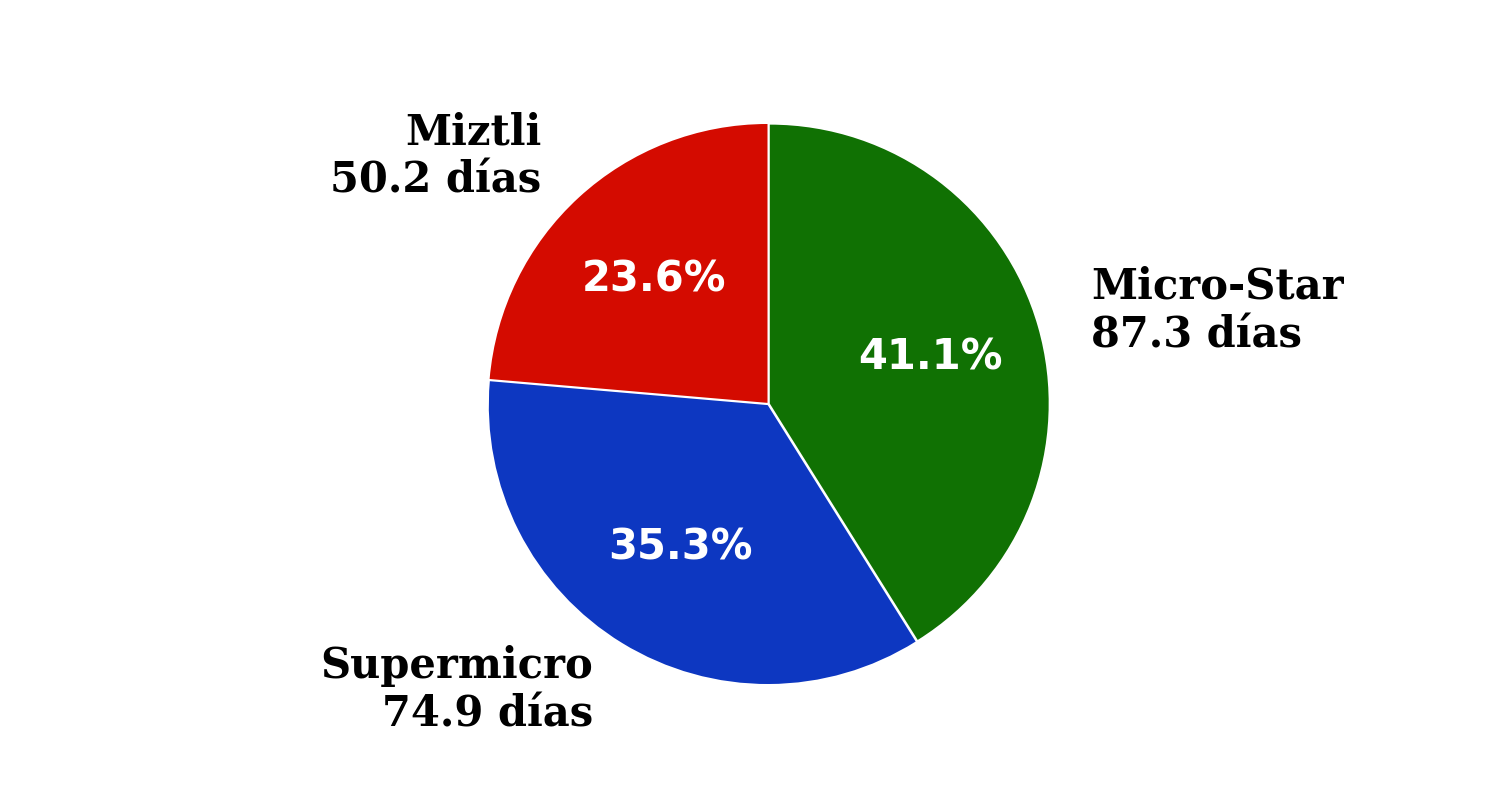
\includegraphics[width=\linewidth]{Imágenes/grafico_tiempo_pastel.png}
    \end{minipage}
    \hfill % Relleno flexible para separarlas
    % --- Gráfica 2: Pasos (Derecha) ---
    \begin{minipage}[b]{0.48\textwidth}
        \centering
        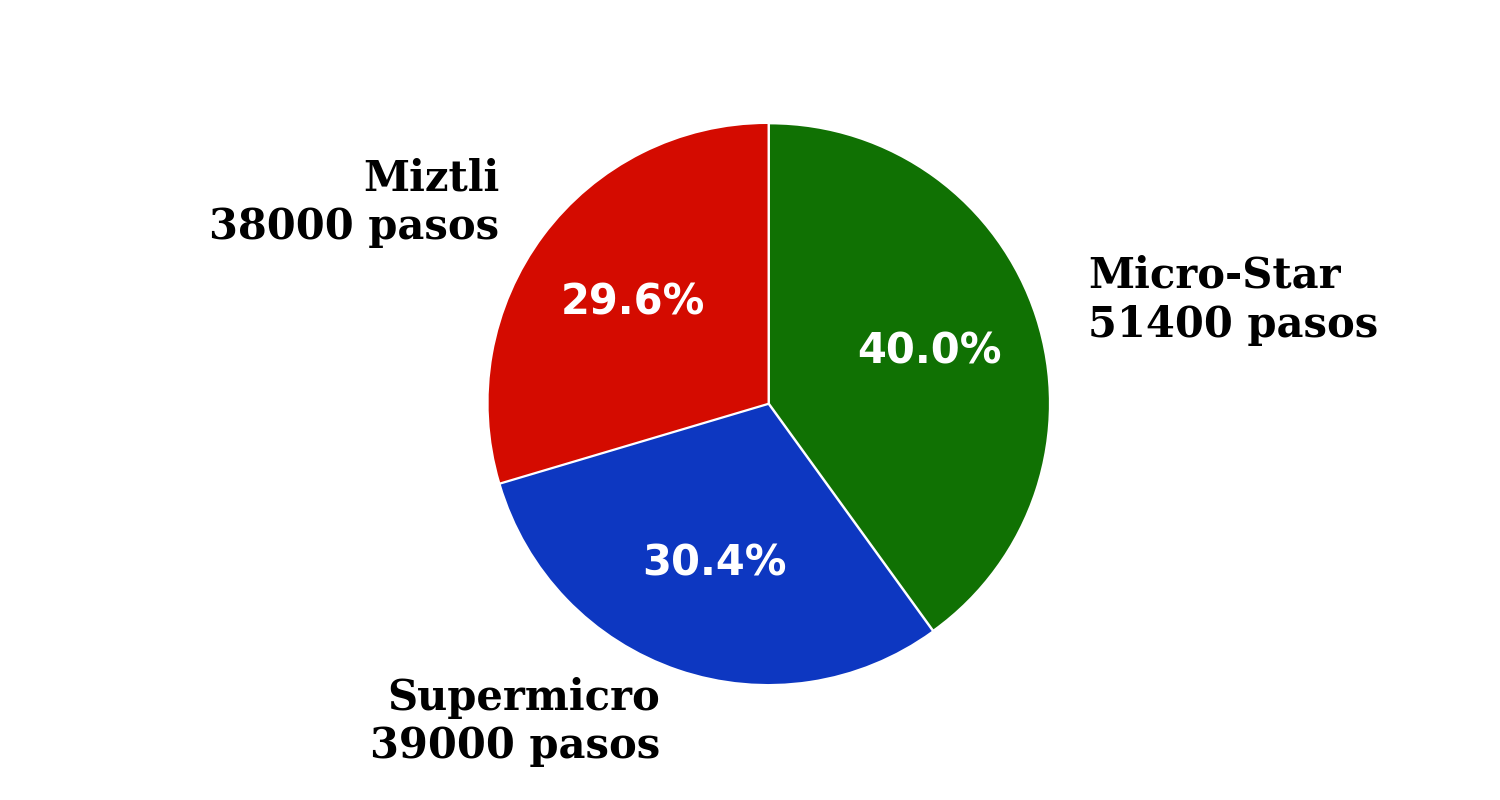
\includegraphics[width=\linewidth]{Imágenes/grafico_pasos_pastel.png}
    \end{minipage}
    \caption[Tiempo de cómputo y pasos MD]{Distribución del tiempo de cómputo (izquierda) y del número de pasos de MD (derecha) entre los diferentes recursos utilizados.}
    \label{fig:tiempo_computo}
\end{figure}

% --- Tabla de Recursos Computacionales (Estilo Cuadrícula) ---
\begin{table}[h]
    \centering
    \footnotesize 
    \begin{threeparttable}
        \caption{Infraestructura de cómputo y rendimiento en la producción de dinámica molecular.}
        \label{tab:recursos_computacionales}
        % Nota los '|' entre las letras para crear las líneas verticales
        \begin{tabular}{|l|c|c|c|}
            \hline
             & \textbf{Supercomputadora} & \textbf{Estación} & \textbf{Estación} \\
             & \textbf{Miztli (DGTIC)} & \textbf{Supermicro AS-5014A} & \textbf{Micro-Star MS-7E26} \\
            \hline
            \hline
            \multicolumn{4}{|c|}{\textbf{Especificaciones de Hardware}} \\
            \hline
            \textbf{Procesador} & 2x Intel Xeon E5-2670v1 & 1x AMD Threadripper & 1x AMD Ryzen 9 \\
             & (por nodo) & Pro 3975WX & 7950X3D \\
            \hline
            \textbf{Núcleos} & \textbf{32 núcleos} (16/nodo) & \textbf{32 núcleos} & \textbf{16 núcleos} \\
            \hline
            \textbf{Hilos} & \textbf{64 hilos} (32/nodo) & \textbf{64 hilos} & \textbf{32 hilos} \\
            \hline
            \textbf{RAM} & \textbf{128 GB} (64/nodo) & \textbf{128 GB} & \textbf{128 GB} \\
            \hline
            \hline
            \multicolumn{4}{|c|}{\textbf{Rendimiento (ORCA 6.1)}} \\
            \hline
            \textbf{\ce{[Cu(H2O)_{40}]^{2+}}} & 38,000 pasos & 8,000 pasos & 14,400 pasos \\
             & (378 pasos/día) & (789 pasos/día) & (807 pasos/día)\\
            \hline
            \textbf{\ce{[Cu(CH3OH)_{40}]^{2+}}} & --- & 31,000 pasos & 37,000 pasos \\
             & & (222 pasos/día) & (236 pasos/día) \\
            \hline
        \end{tabular}
        \begin{tablenotes}
            \footnotesize
            \item Nota: El rendimiento reportado corresponde a una única réplica evaluada bajo condiciones de ocupación total del equipo (ejecutando dos réplicas simultáneas que comparten y compiten por los recursos físicos del procesador). Por lo tanto, la producción total del equipo en este escenario de carga máxima equivale al doble del valor individual mostrado.
        \end{tablenotes}
    \end{threeparttable}
\end{table}

\section{Métodos de análisis estructural}

\subsection{Función de distribución radial}

La Función de Distribución Radial (RDF, por sus siglas en inglés) es una herramienta estadística en el análisis estructural de sistemas moleculares; mide la probabilidad de encontrar un átomo de tipo $X$ a una distancia radial $\mathbf{r}$ respecto a un átomo de referencia $M$. Su definición formal se establece como el cociente entre la densidad local de partículas, $\rho(\mathbf{r})$, y la densidad numérica promedio del sistema, $\rho_0$. 

\begin{equation}
g_{M -x}(\mathbf{r}) = \frac{\rho(\mathbf{r})}{\rho_0} \label{eq:densidad_rdf}
\end{equation}

Para determinar la densidad local, se selecciona un átomo central y se contabiliza el número de partículas, denominado $N(\mathbf{r})$, que se encuentran confinadas dentro de un cascarón esférico de radio $\mathbf{r}$ y un espesor finito $\Delta \mathbf{r}$, tal como se esquematiza en la Figura \ref{fig:esquema_rdf}.

\begin{figure}[H]
    \centering
    % Primera imagen (Izquierda)
    \begin{minipage}{0.58\textwidth}
        \centering
        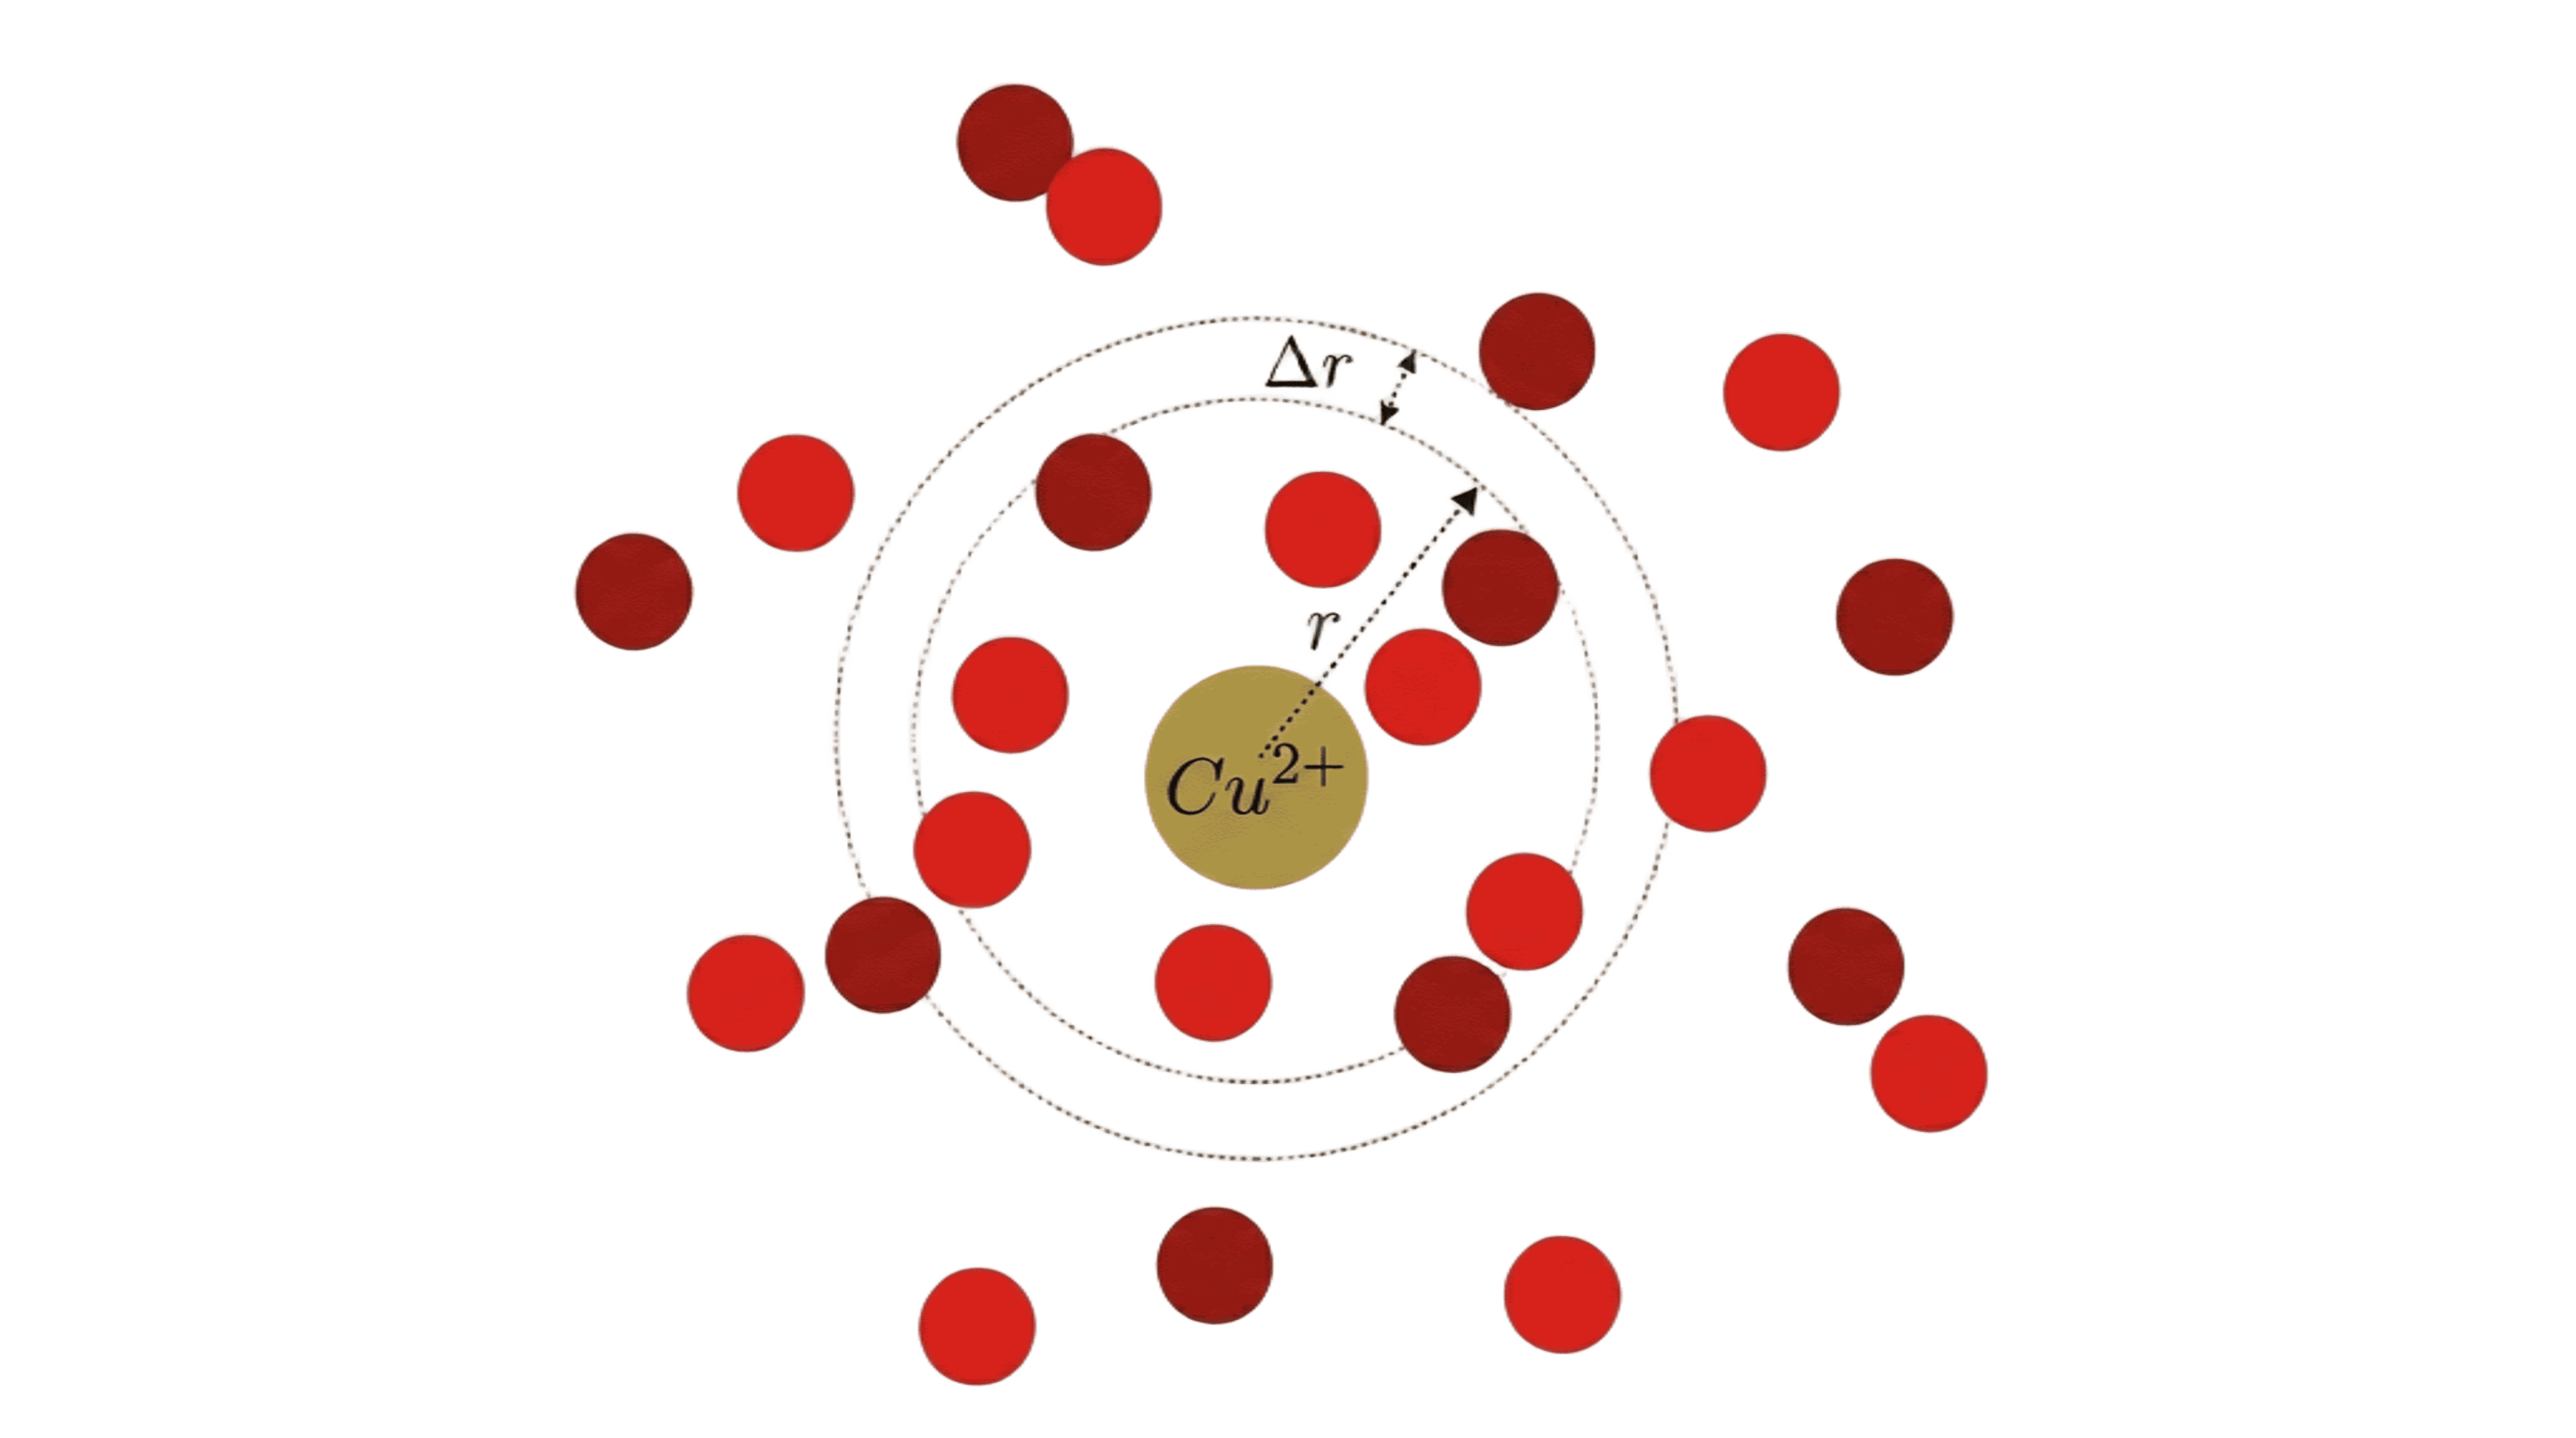
\includegraphics[width=\textwidth]{Imágenes/RDF-5.png}
    \end{minipage}
    \hfill % Espacio flexible entre las dos imágenes
    \begin{minipage}{0.38\textwidth}
        \centering
        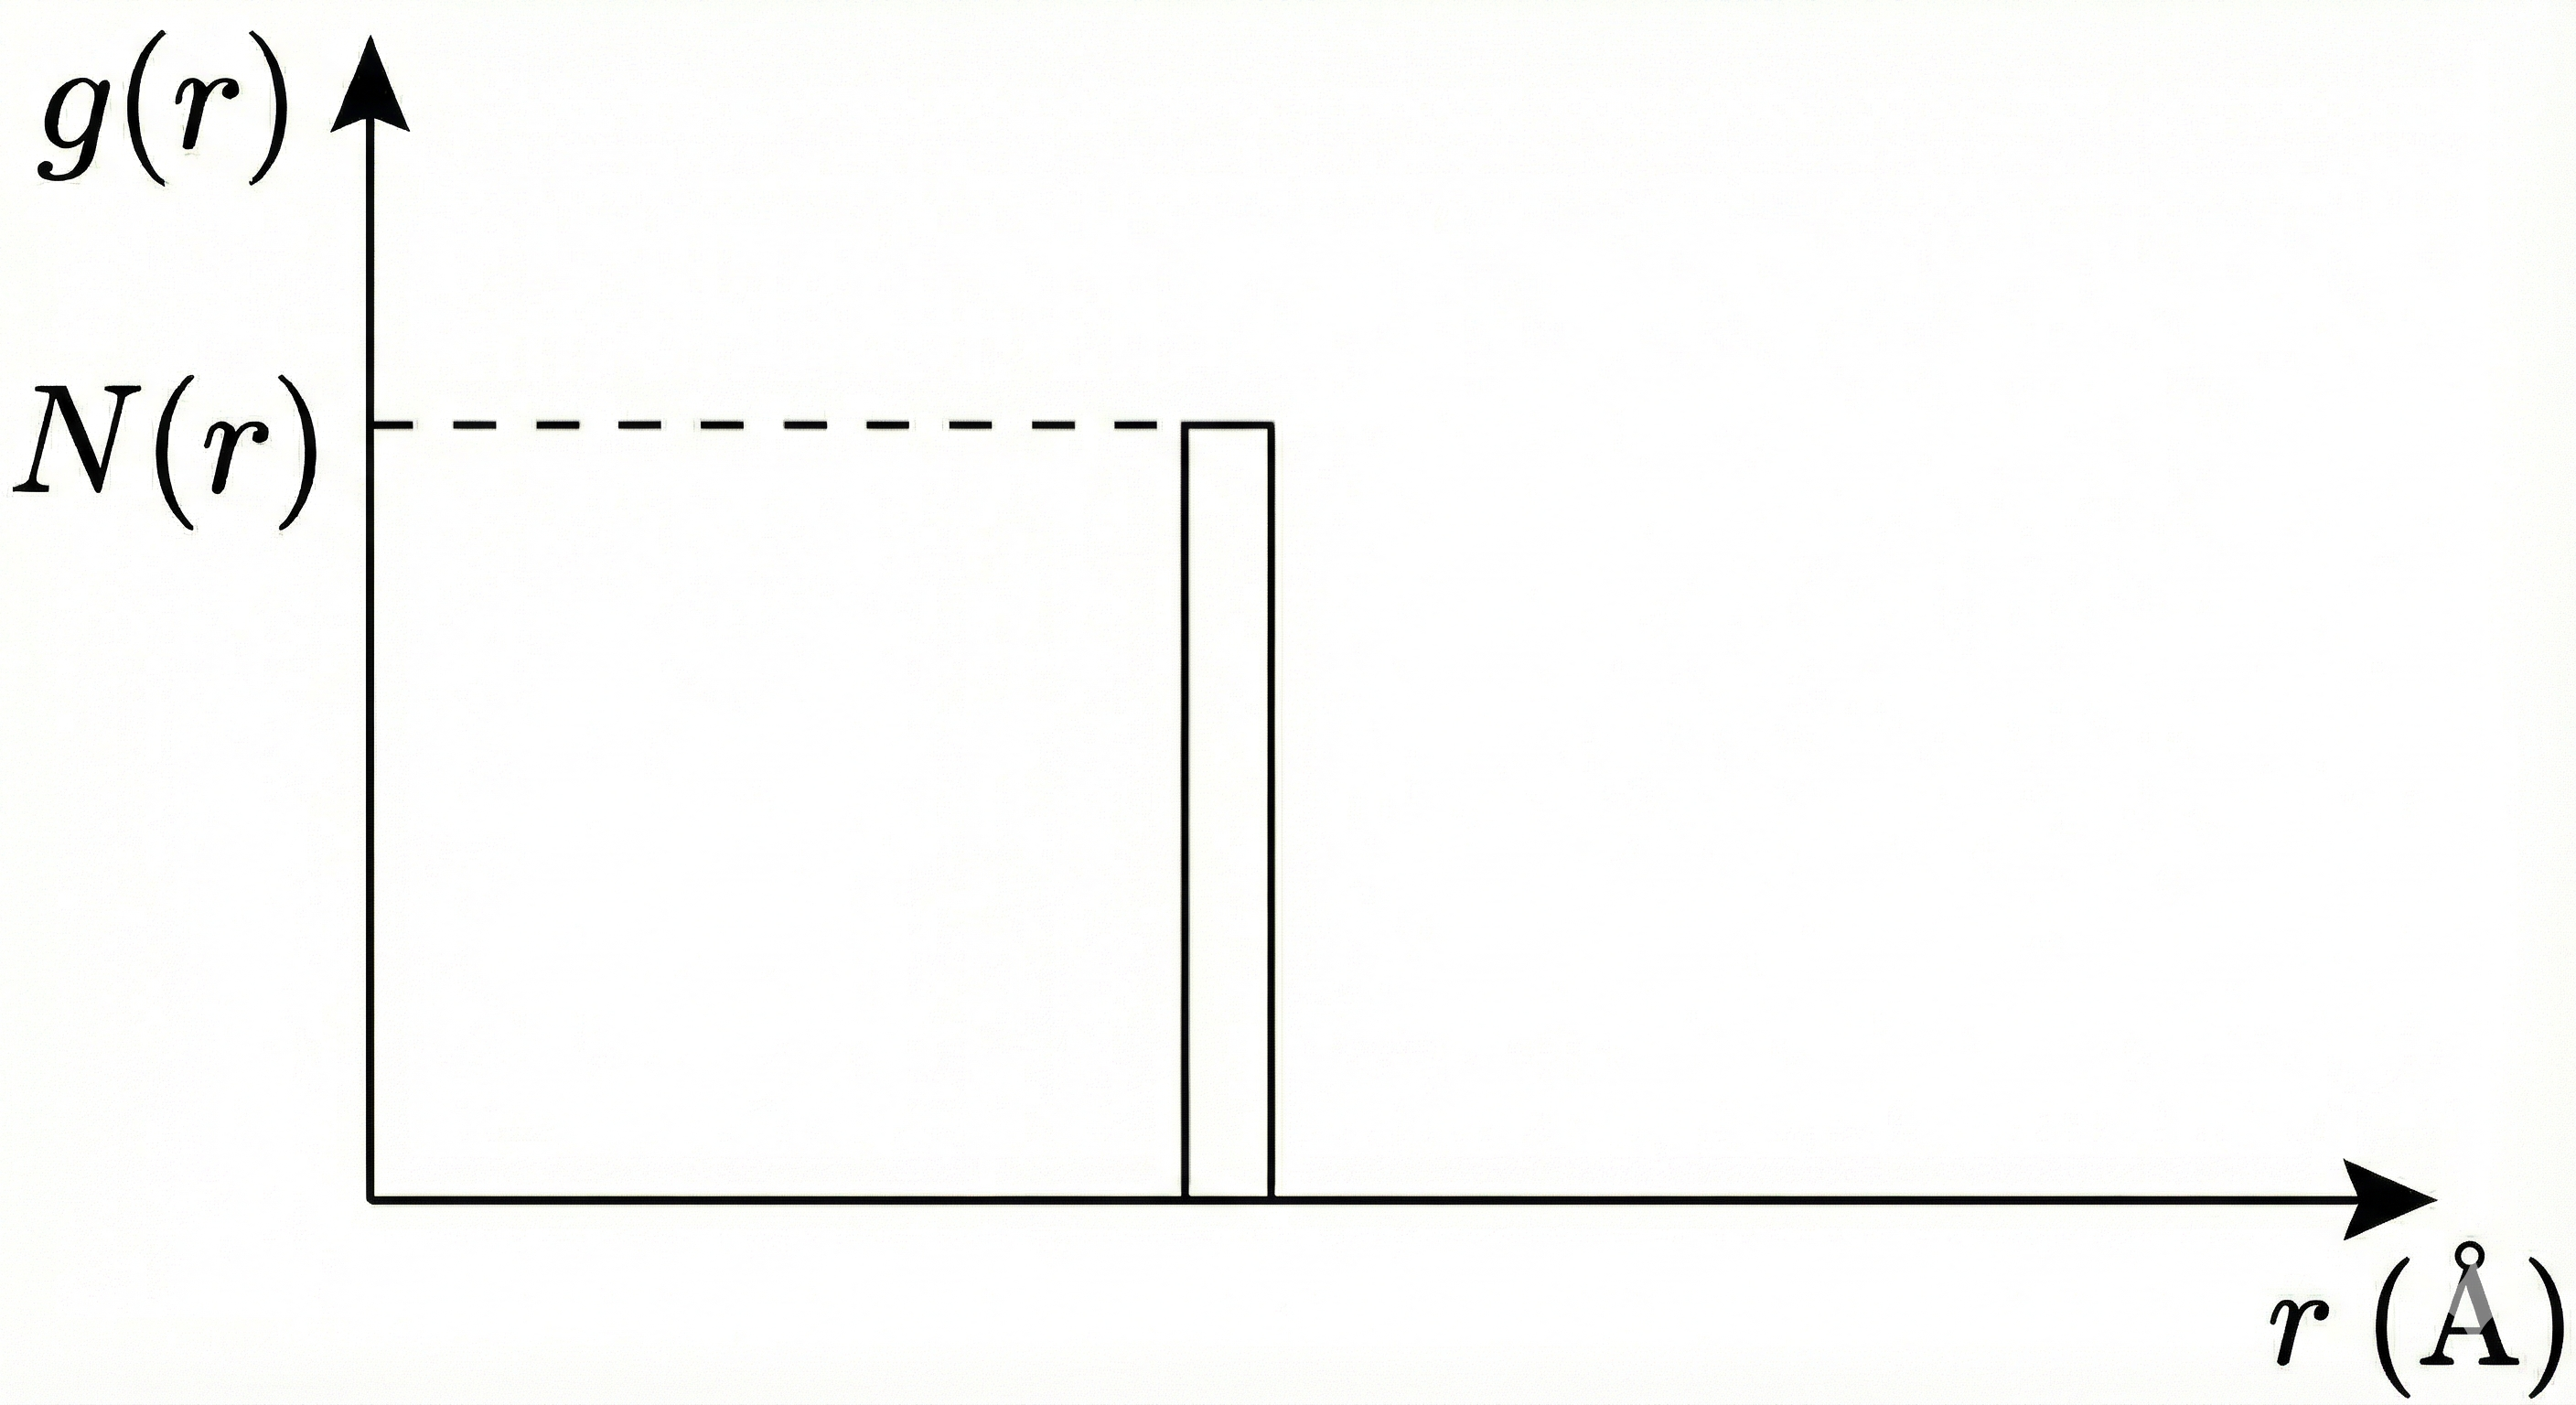
\includegraphics[width=\textwidth]{Imágenes/RDF-6.png}
       
    \end{minipage}
    \caption[Representación esquemática para el cálculo de la RDF]{Representación esquemática para el cálculo de la RDF. Se ilustra el átomo de referencia central, la distancia radial $\mathbf{r}$ y el cascarón esférico de grosor $\Delta \mathbf{r}$ donde se evalúa el conteo de partículas $N(\mathbf{r})$.}
     \label{fig:esquema_rdf}
\end{figure}

Se desarrolló un programa en Python que calcula la densidad local basándose en el volumen geométrico exacto de las capas esféricas discretizadas. De esta manera, la expresión teórica general utilizada para determinar $g(\mathbf{r})$ en el intervalo de distancia $(\mathbf{r}, \mathbf{r} + \Delta \mathbf{r})$ queda definida como:
\begin{equation}
    g(\mathbf{r}) = \frac{\langle N(\mathbf{r}, \Delta \mathbf{r}) \rangle}{\frac{4}{3}\pi \rho_{0} \left[ (\mathbf{r} + \Delta \mathbf{r})^3 - \mathbf{r}^3 \right]}
    \label{eq:rdf_general}
\end{equation}

En esta expresión, el término $\langle N(\mathbf{r}, \Delta \mathbf{r}) \rangle$ representa el número promedio de partículas encontradas dentro de una capa esférica de grosor $\Delta \mathbf{r}$ a lo largo de los pasos de simulación analizados. El denominador normaliza este conteo utilizando el volumen real de dicha cáscara esférica y por la densidad numérica, $\rho_{0}$. Los valores de $\rho_{0}$ utilizados en este trabajo se resumen a continuación. 

\begin{table}[htbp]
    \centering
    \caption{Densidades numéricas ($\rho_0$) de los solventes puros a 300 K empleadas para la normalización de las funciones de distribución radial.}
    \label{tab:densidades_solventes}
    \begin{tabular}{llccc}
        \hline
        \textbf{Solvente} & \textbf{Presión} & \textbf{Densidad} & \textbf{$\rho_0$} & \textbf{Ref} \\
        & & \textbf{(g/cm$^3$)} & \textbf{(\AA$^{-3}$)} & \\ \hline
        Agua líquida & 101,325 Pa     & 0.9965714 & 0.03331335 & \cite{rumble2017crc, marsh1987recommended} \\
        Metanol & 101,325 Pa & 0.78459  & 0.014746 & \cite{NIST_WebBook_Fluids} \\ \hline
    \end{tabular}
\end{table}

\subsection{Número de coordinación acumulado}

De manera complementaria al perfil de distribución, se evalúa el Número de Coordinación Acumulado, denotado como $n(\mathbf{r})$. Esta métrica cuantifica el número total promedio de átomos vecinos que se encuentran confinados dentro de una esfera de radio $r$ centrada en el átomo de referencia. Analíticamente, esta magnitud corresponde a la integración de la función de distribución radial, ponderada por la densidad numérica del sistema y el elemento diferencial de volumen esférico:

\begin{equation}
    n(\mathbf{r}) = 4\pi \rho_0 \int_0^{\mathbf{r}} g(\mathbf{r}') (\mathbf{r}')^2 d(\mathbf{r}')
    \label{eq:cn_integral}
\end{equation}

En consistencia con el algoritmo discretizado empleado para la Ec. \ref{eq:rdf_general}, el cálculo computacional de $n(\mathbf{r})$ no requiere una integración numérica compleja, sino que se obtiene mediante la suma acumulativa directa del conteo promedio de partículas por capa. Dado que el término $\langle N(\mathbf{r}, \Delta \mathbf{r}) \rangle$ ya representa la población promedio en cada cascarón esférico individual, el número de coordinación a una distancia $\mathbf{r}$ queda definido por la suma de estas contribuciones desde el origen hasta el radio de corte:
\begin{equation}
    n(\mathbf{r}) = \sum_{\mathbf{r}'=0}^{\mathbf{r}} \langle N(\mathbf{r}', \Delta \mathbf{r}') \rangle
    \label{eq:cn_discreto}
\end{equation}

Esta formulación permite determinar la ocupación de las distintas esferas de solvatación, identificando la cantidad de vecinos inmediatos al evaluar $n(\mathbf{r})$ en los mínimos locales de $g(\mathbf{r})$.

\subsection{Función de distribución angular}

La Función de Distribución Angular (ADF, por sus siglas en inglés) se emplea para cuantificar la disposición espacial de tripletes atómicos. Específicamente, esta métrica evalúa la probabilidad de ocurrencia de un ángulo $\theta_{ijk}$ formado entre un átomo central y sus pares adyacentes. La importancia de la ADF radica en su capacidad para revelar el entorno de coordinación y las hibridaciones presentes, ya que la posición y morfología de sus picos actúan como una huella dactilar de la geometría local del material. 

Se desarrollaron algoritmos en Python que evalúan iterativamente las trayectorias de dinámica molecular. El programa identifica los ligandos situados dentro de la primera esfera de solvatación, delimitada por un radio de corte $r_{cut}$  y determina el ángulo $\theta$ a partir del producto escalar entre los vectores de posición relativos $\mathbf{r}_{ij}$ y $\mathbf{r}_{ik}$, de acuerdo con la relación geométrica:

\begin{equation}
    \theta = \arccos \left( \frac{\mathbf{r}_{ij} \cdot \mathbf{r}_{ik}}{|\mathbf{r}_{ij}| |\mathbf{r}_{ik}|} \right)
    \label{eq:angulo_adf}
\end{equation}

Posteriormente, la recolección estadística de estos valores permite la construcción de histogramas de frecuencia normalizados que, tras aplicar un suavizado numérico, revelan la función de densidad de probabilidad $P(\theta)$ característica de cada sistema.

\section{Cúmulo \ce{[Cu(H2O)40]^{2+}}}

El análisis estructural de este sistema se realizó a partir de la trayectoria compuesta formada por la concatenación de las réplicas independientes A, B, C y D descritas en la Tabla \ref{tab:replicas_md}. Este enfoque se fundamenta en la hipótesis ergódica, discutida en la sección \ref{section-Termostatos}, que garantiza la equivalencia entre el promedio temporal de una trayectoria suficientemente larga y el promedio estadístico sobre un conjunto de configuraciones independientes. Dado que las propiedades estructurales de interés dependen únicamente del muestreo configuracional del sistema y no de la continuidad temporal entre las réplicas, su combinación resulta estadísticamente válida y permite obtener estimaciones más robustas con el tiempo total de simulación disponible (30.20 ps, véase Tabla \ref{tab:replicas_md}). Los resultados se presentan en las Figuras \ref{fig:rdf_agua} y \ref{fig:adf_agua}.

\subsection*{Función de distribución radial e hidratación en primera esfera}

% --- RDF AGUA ---
\begin{figure}[H]
    \centering
    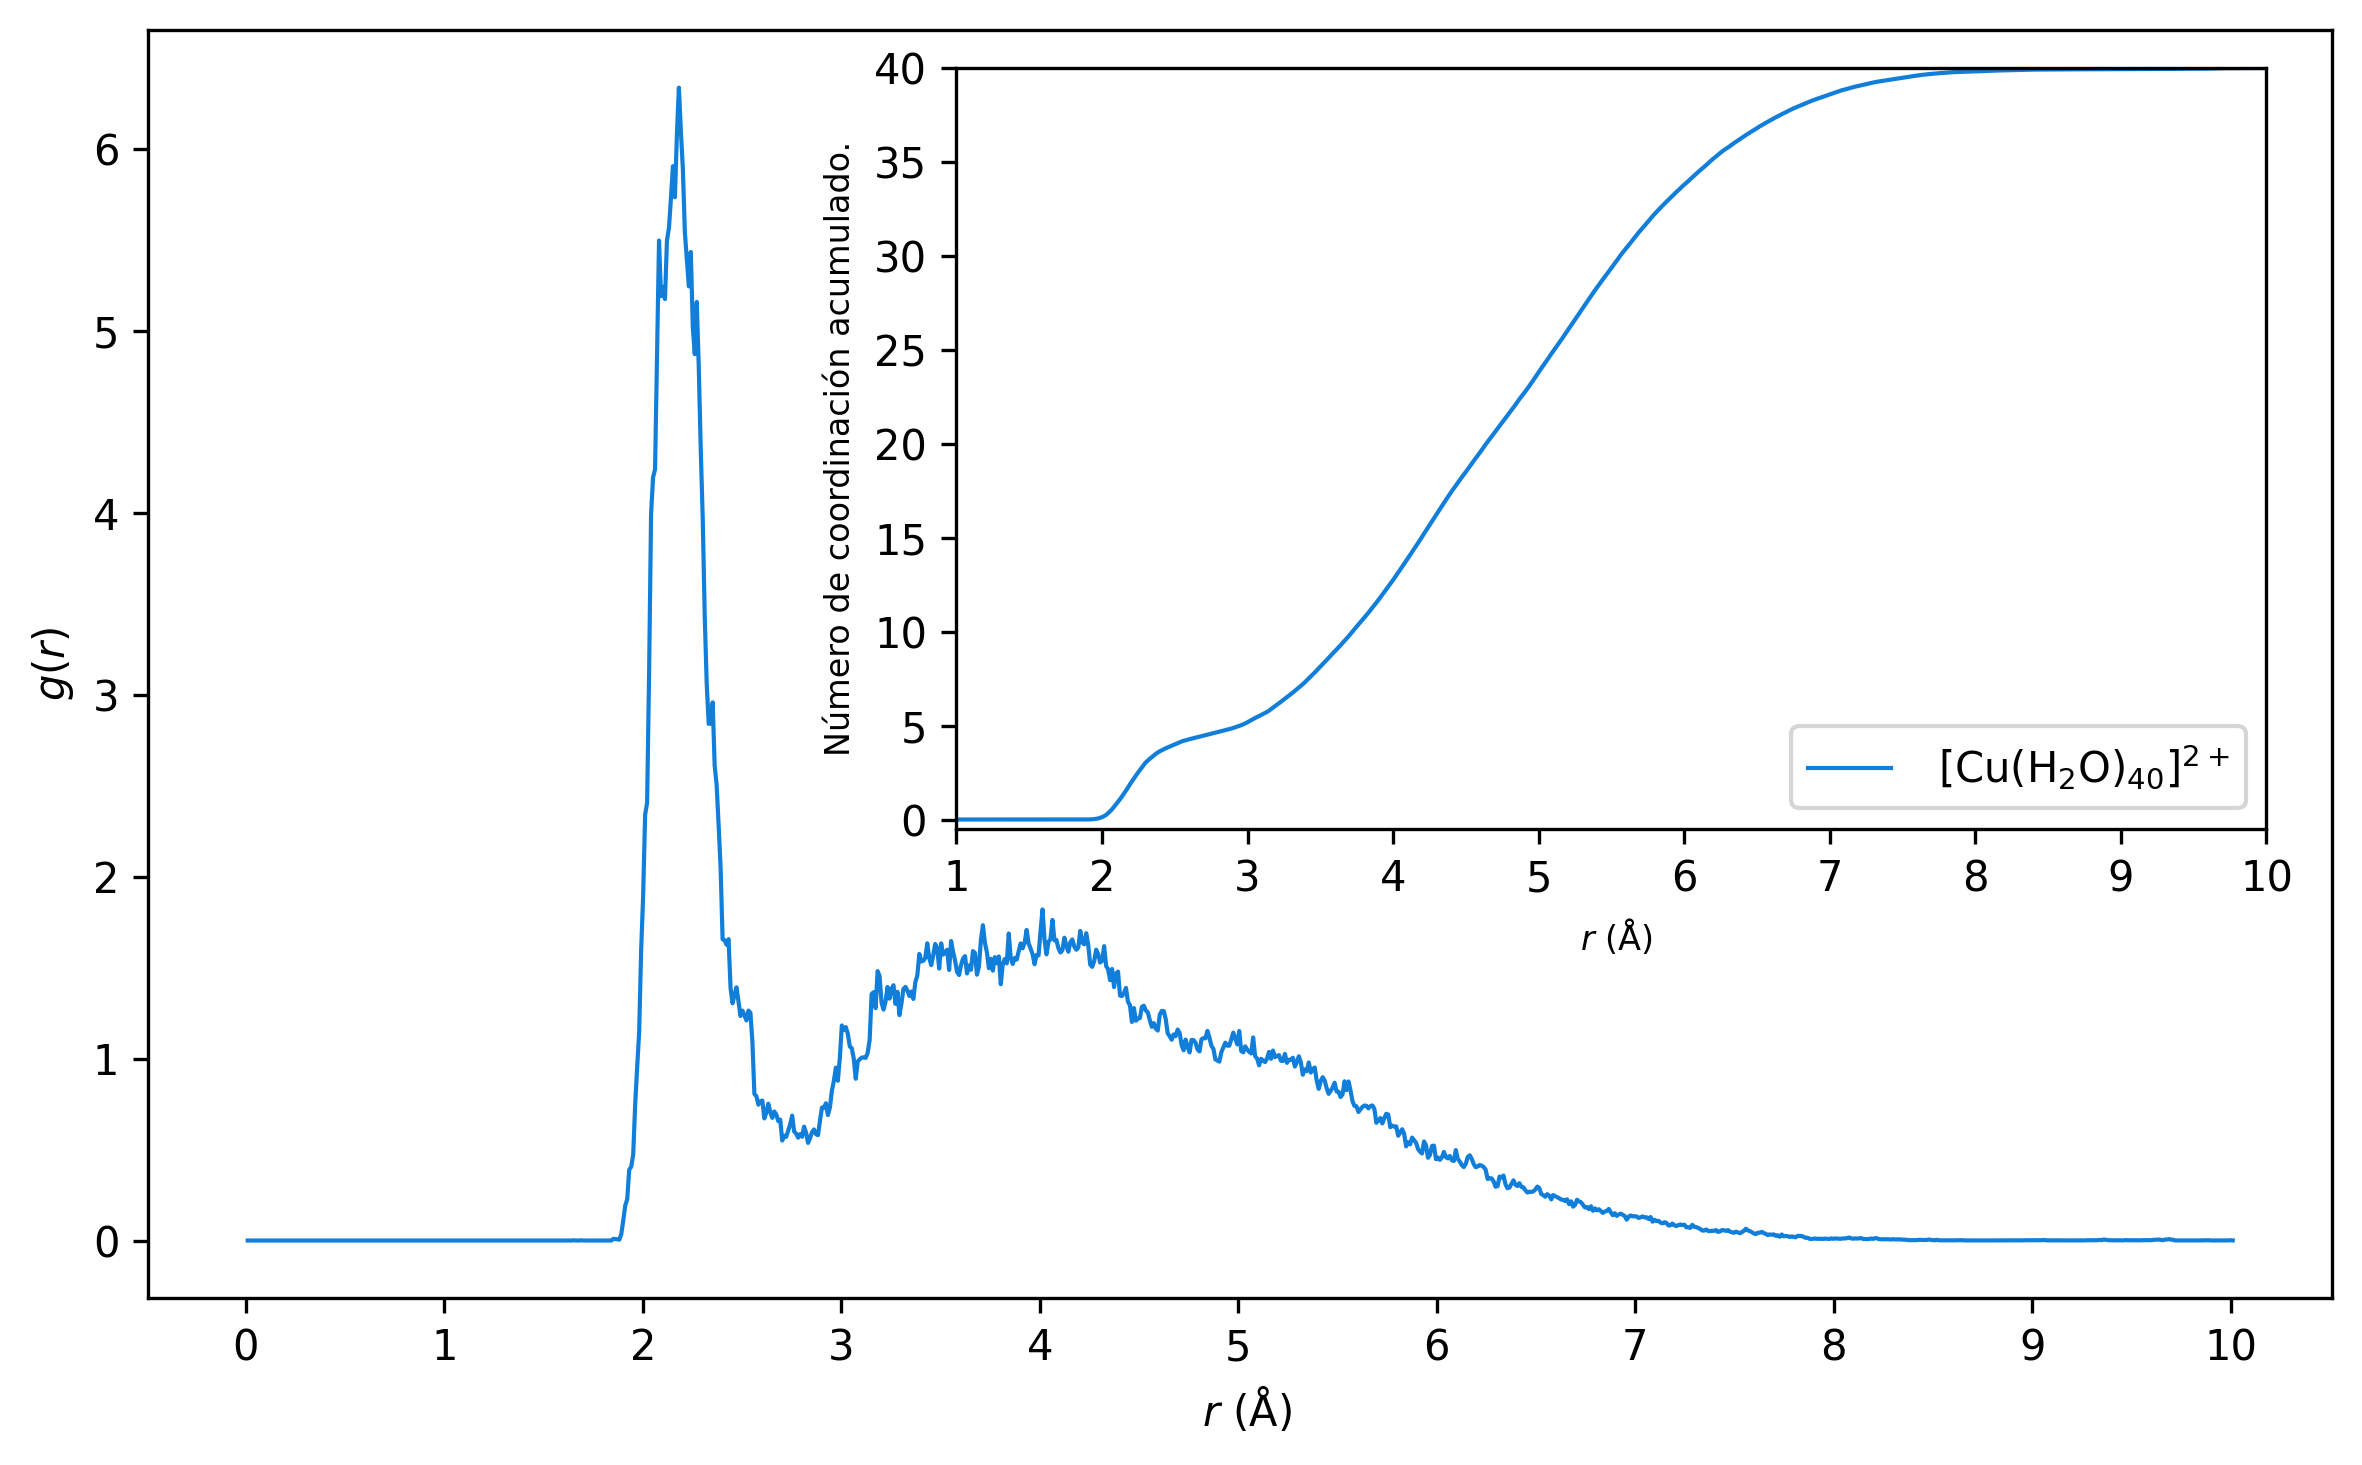
\includegraphics[width=0.95\textwidth]{Imágenes/RDF-OUTPUT-HISTOGRAMA-AGUA.png}
    \caption[RDF para el cúmulo \ce{[Cu(H2O)40]^{2+}}]{Función de distribución radial (RDF) obtenida para el sistema \ce{[Cu(H2O)40]^{2+}} a partir de la simulación de dinámica molecular.}
    \label{fig:rdf_agua}
\end{figure}

La RDF del par \ce{Cu-O} presenta un primer pico principal centrado en $(r,\, g(r)) = (2.182\,\text{Å},\, 6.339)$, que corresponde a la distancia más probable entre el ion y los oxígenos de las moléculas de agua de la primera esfera de coordinación. El perfil de este pico es notablemente asimétrico: el flanco izquierdo sube de forma abrupta desde $r \approx 1.85$ Å, mientras que el flanco derecho desciende de manera más gradual hasta alcanzar el mínimo local en $(r,\, g(r)) = (2.833\,\text{Å},\, 0.537)$. Esta asimetría es característica de los sistemas donde la interacción  electrostática impone un límite de acercamiento muy preciso, pero permite cierta flexibilidad en las distancias de separación.

El hecho de que el mínimo entre el primer y el segundo pico no sea cero confirma que la primera esfera de coordinación no es rígida y que eventos de intercambio de ligandos ocurren durante la trayectoria. Un valor de $g(r) > 0$ en el mínimo indica que, en alguna fracción de los pasos de simulación, una molécula de agua se encuentra en esa zona de transición, lo que evidencia la ocurrencia de eventos de intercambio de ligandos entre las esferas de solvatación durante la dinámica.

\subsection*{Segunda esfera de solvatación}

La segunda esfera de coordinación se manifiesta como un pico ancho, con morfología de meseta, en el intervalo aproximado $r \in [3.71,\, 4.32]$ Å, con un máximo local en $(r,\, g(r)) = (4.014\, Å,\, 1.820)$. A diferencia del primer pico, este carece de un flanco descendente bien definido: la función $g(r)$ decae de forma continua desde $r \approx 4.32$ Å hasta alcanzar el valor de referencia $g(r) \approx 1$ en el intervalo $r \in [4.88,\, 5.27]$ Å, sin exhibir un segundo mínimo localizado.

El decaimiento de $g(r)$ hacia cero para valores grandes de $r$ es una consecuencia directa de la naturaleza finita del cúmulo simulado: más allá de cierto radio, $N(r) = 0$, es decir, a esa distancia la probabilidad de encontrar moléculas de solvente adicionales en torno al ion es prácticamente nula. Como se mencionó al inicio de este capítulo, la metodología de cúmulos finitos empleada en estudios previos del grupo ha demostrado ser capaz de reproducir con 
alta precisión propiedades estructurales y dinámicas medidas experimentalmente en el líquido, tales como la RDF, el número de coordinación, los espectros EXAFS y el espectro vibracional.

\subsection*{Número de coordinación acumulado}

Para determinar el número de moléculas que constituyen la primera esfera de coordinación, se evalúa el número de coordinación acumulado $n(r)$ en el primer mínimo de la RDF, de acuerdo con la Ec. \ref{eq:cn_discreto}. Se obtiene $n(2.833\,\text{Å}) = 4.729$. Es importante notar que en esta región no se observa la meseta horizontal característica que
presentan los sistemas con un número de coordinación fijo y bien definido (véase el inset de la figura \ref{fig:rdf_agua}). La ausencia de dicha meseta indica que el número de ligandos en la primera esfera de coordinación no es constante a lo largo de la trayectoria, sino que el complejo oscila dinámicamente entre estados con 4, 5 y 6 moléculas de agua coordinadas, fenómeno que se discutirá con mayor detalle al analizar la distribución angular.

Adicionalmente, es posible calcular la distribución del número de coordinación a lo largo de la trayectoria, es decir, la frecuencia con la que el ion se encuentra coordinado por 4, 5 o 6 moléculas de agua. Para esto, se cuenta el número de moléculas dentro del radio de corte $r = 2.833$ Å en cada paso de la simulación y se construye un histograma de frecuencias. Los resultados son consistentes con el número de coordinación acumulado y se muestran en la Figura \ref{fig:nc_distribution_water}.

\begin{figure}[htbp]
    \centering
    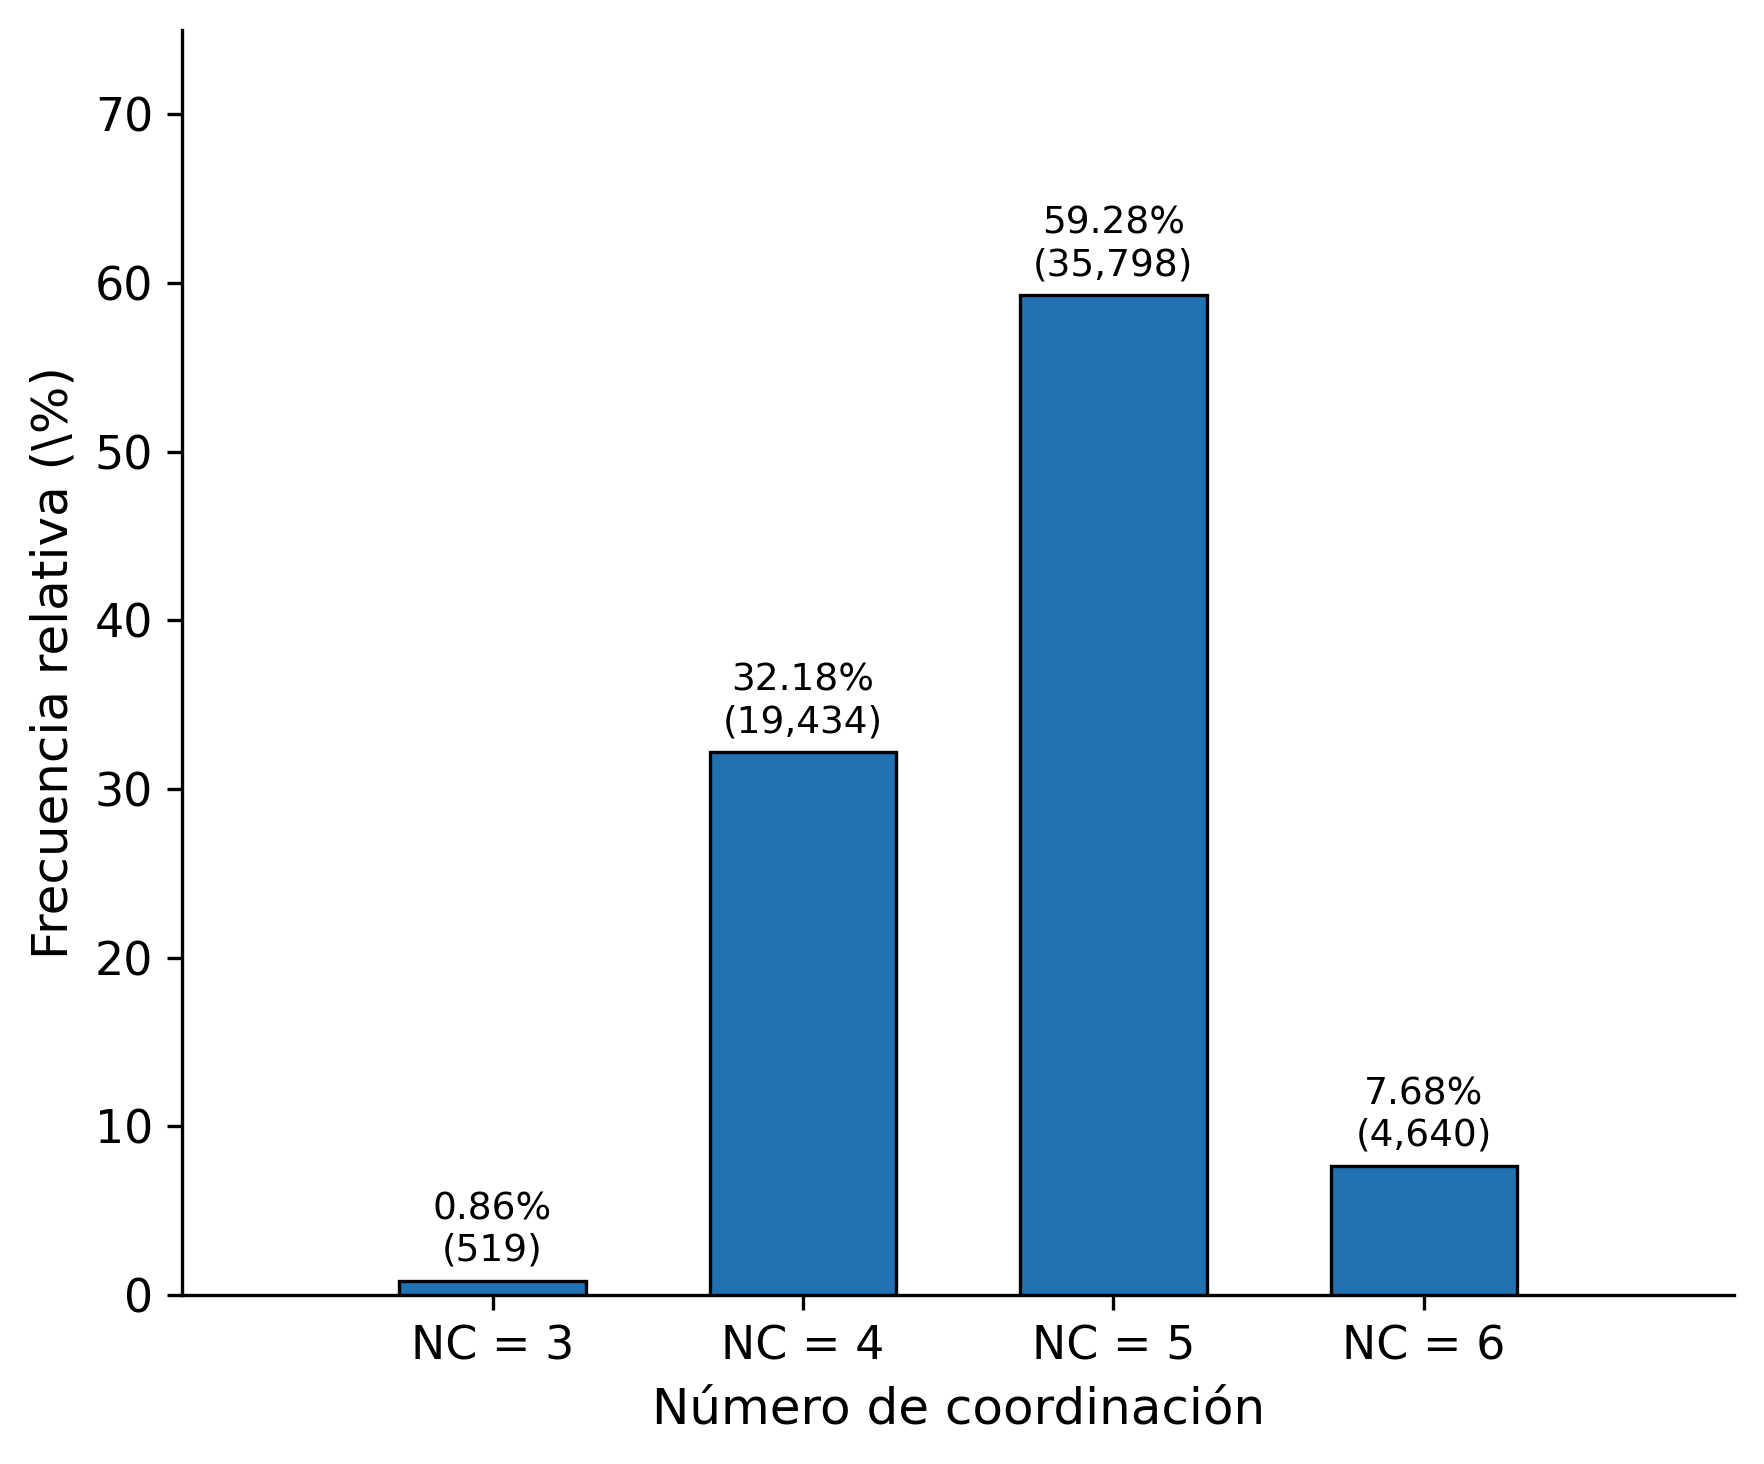
\includegraphics[width=0.6\textwidth]{Imágenes/nc_distribution_agua.png}
    \caption[Frecuencia del número de coordinación para \ce{[Cu(H2O)40]^{2+}}]{Frecuencia del número de coordinación del ion obtenida a partir de la trayectoria (60\,391 frames, $r = 2.833$~\AA).}
    \label{fig:nc_distribution_water}
\end{figure}

\subsection*{Función de distribución angular y geometría de coordinación}

Con el propósito de complementar la información estructural obtenida de la RDF, se calculó la función de distribución angular empleando el mismo radio de corte utilizado para el número de coordinación, $r_{cut} = 2.833$~\AA{}, de modo que el análisis angular caracterice exclusivamente la primera esfera de coordinación. El resultado se muestra en la Figura \ref{fig:adf_agua}.

% --- ADF AGUA ---
\begin{figure}[H]
    \centering
    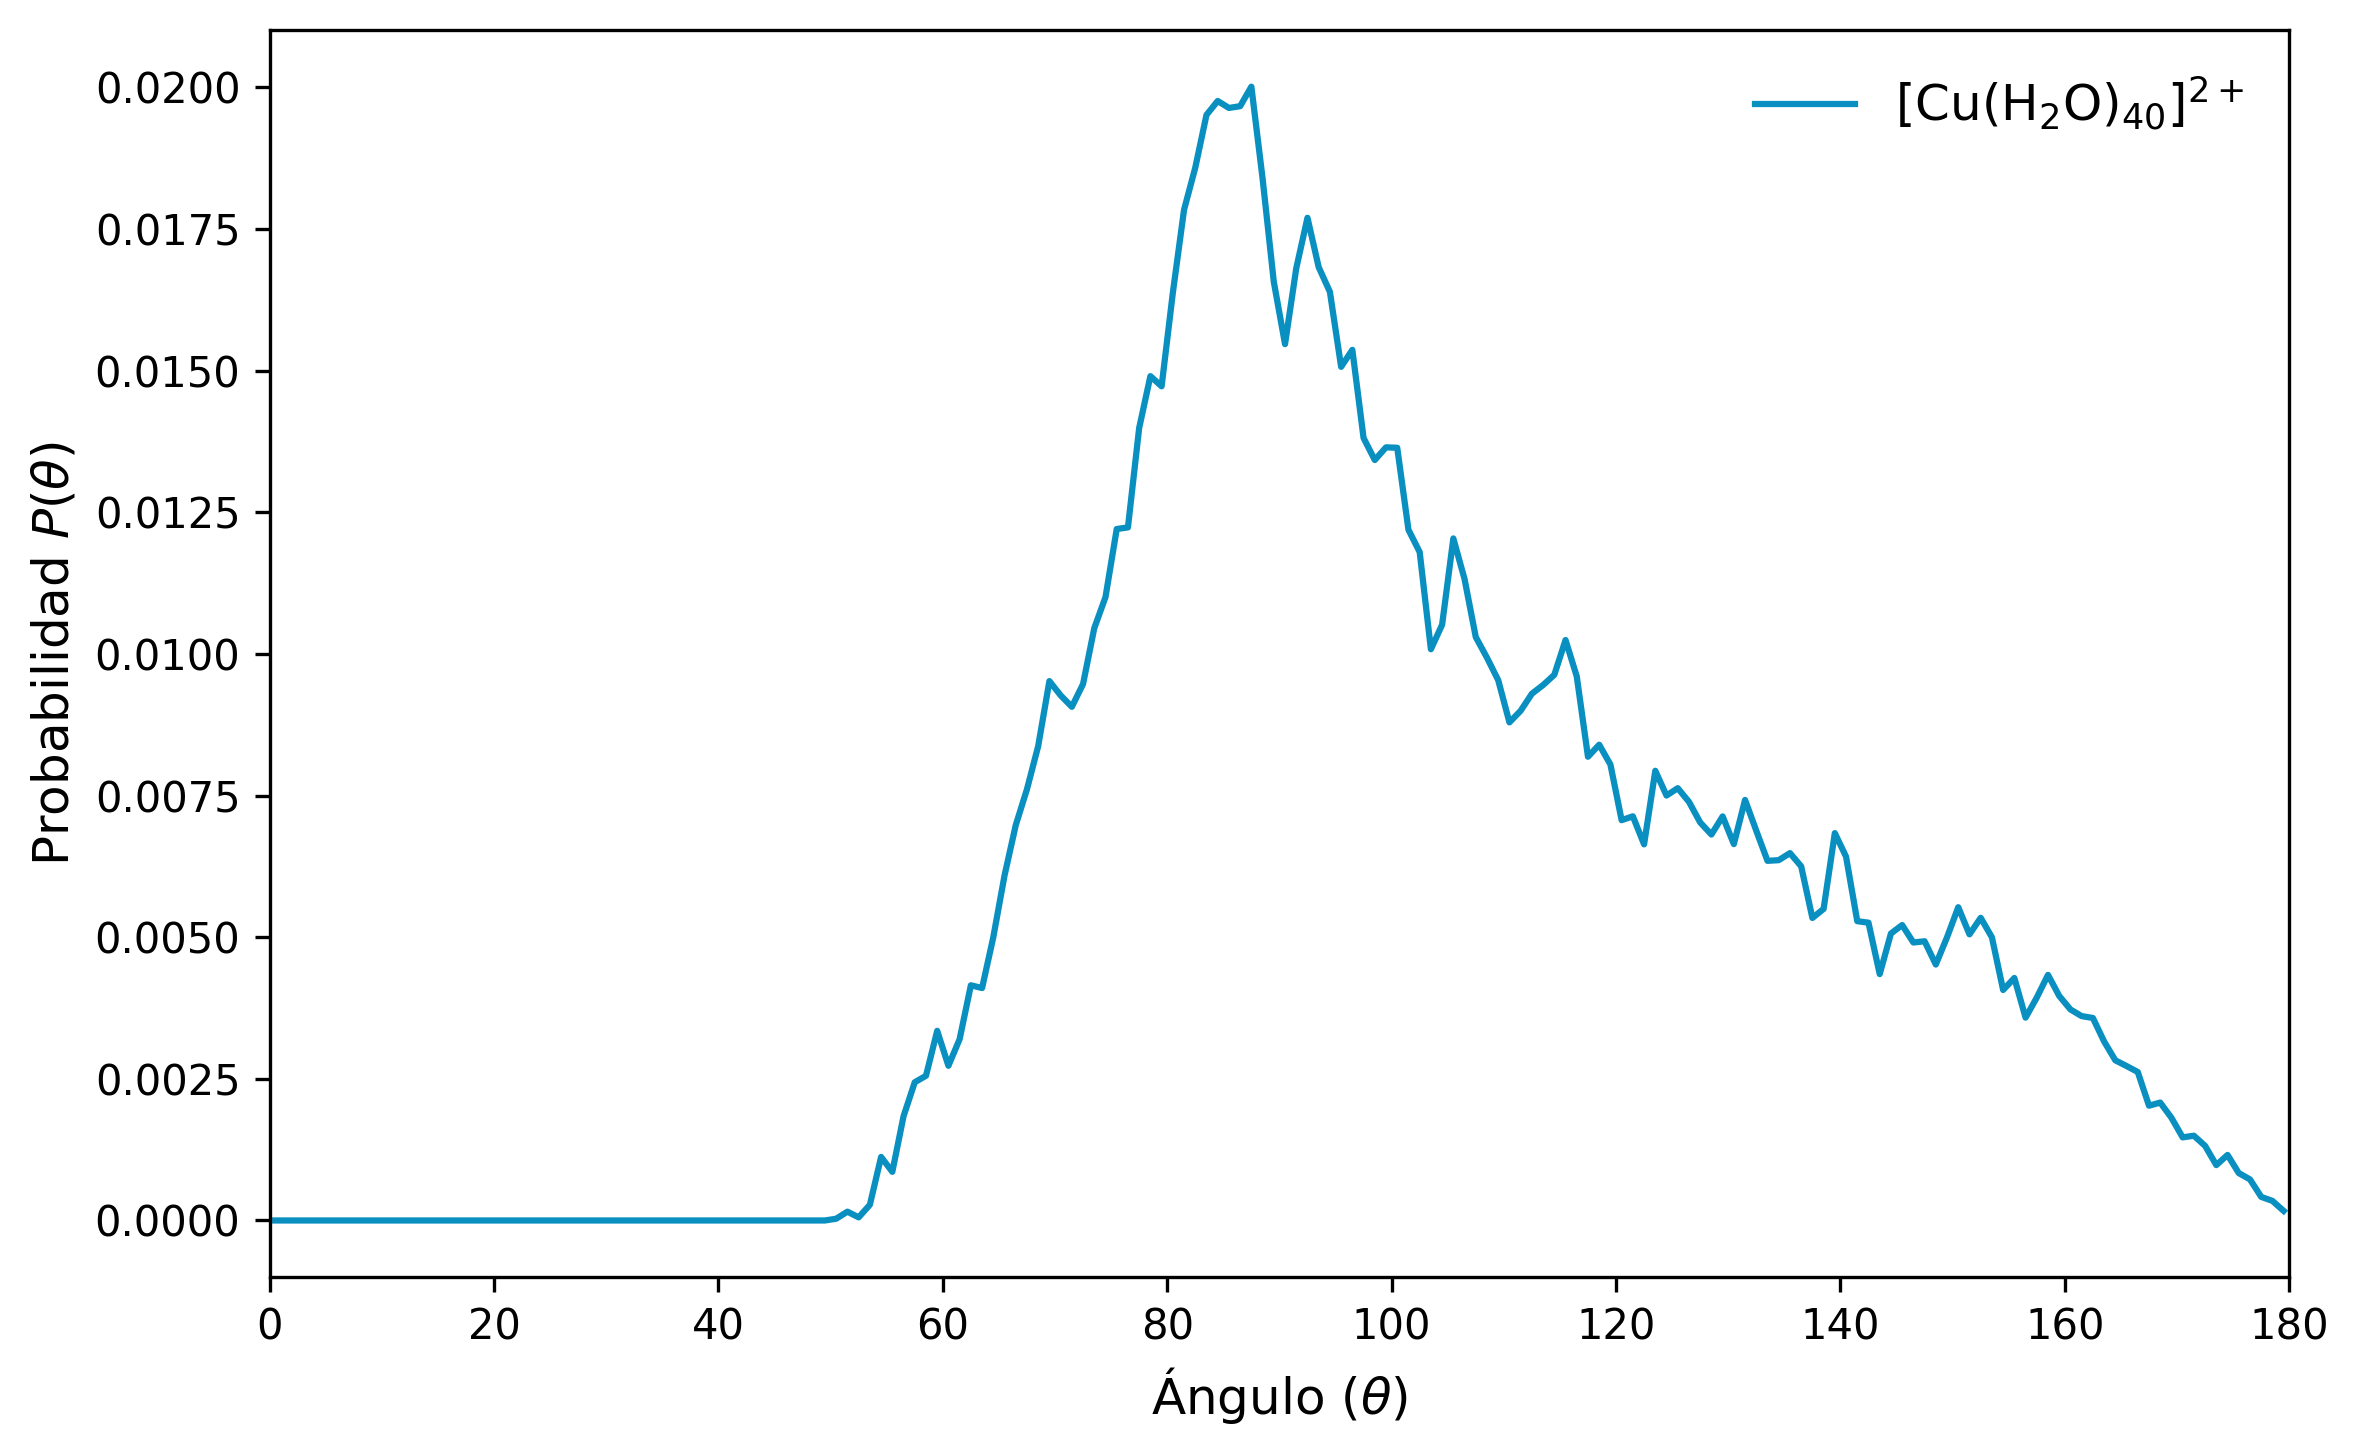
\includegraphics[width=0.95\textwidth]{Imágenes/ADF-OUTPUT-H2O.png}
    \caption[ADF para \ce{[Cu(H2O)40]^{2+}}]{Función de distribución angular (ADF) obtenida para el sistema \ce{[Cu(H2O)40]^{2+}} a partir de la simulación de dinámica molecular.}
    \label{fig:adf_agua}
\end{figure}

El perfil de la ADF revela zonas de mayor densidad de probabilidad en torno a los siguientes ángulos: $\theta \approx 87.5^\circ$, $92.5^\circ$, $105.5^\circ$, $115.5^\circ$, $123.5^\circ$, $139.5^\circ$, $145.5^\circ$ y $152.5^\circ$. El rasgo más relevante del espectro angular es la presencia de un pico dominante en $\theta \approx 87^\circ$, acompañado de la práctica ausencia de densidad de probabilidad en la región de $\theta \approx 180^\circ$. Esta distribución es incompatible con una geometría octaédrica regular, la cual debería manifestarse con dos características igualmente prominentes: una banda centrada en $\sim 90^\circ$, correspondiente a los ángulos cis, y otra en $\sim 180^\circ$, correspondiente a los ángulos trans. La ausencia casi completa de esta segunda banda descarta la geometría octaédrica como estado dominante del sistema. En cambio, el perfil observado es coherente con una geometría de pirámide cuadrada: los cuatro ligandos ecuatoriales generan ángulos \ce{O-Cu-O} cercanos a $90^\circ$, mientras que los ángulos ecuatorial axiales también caen en esa misma región angular. Los únicos ángulos que en un octaedro serían trans (180°) se encuentran aquí desplazados hacia la región de $145^\circ$--$152^\circ$, lo que indica que la primera esfera adopta una geometría de pirámide cuadrada distorsionada en la que los ligandos ecuatoriales opuestos no se encuentran en disposición lineal.

Con el propósito de corroborar esta interpretación, se realizó una inspección visual de la trayectoria. Para facilitar el análisis geométrico, se generó una trayectoria reducida conservando únicamente el \ce{Cu^{2+}} y los oxígenos dentro del radio de corte, cuya visualización cuadro a cuadro con el programa Molden \cite{Schaftenaar2000} permitió seguir directamente la evolución temporal de la primera esfera de coordinación.

De esta inspección se desprende que la geometría fluctúa de manera continua entre tres disposiciones recurrentes, ilustradas en la Figura \ref{fig:geom_repr_agua}. La más frecuente es la \textbf{pirámide cuadrada} ($C_{4v}$), con cuatro ligandos ecuatoriales a distancias sensiblemente menores que el ligando axial, rasgo que constituye la manifestación directa del efecto Jahn-Teller  inherente a la configuración electrónica $d^9$ del \ce{Cu^{2+}}. Las otras dos geometrías corresponden a momentos en que el número de ligandos se reduce a cuatro: la \textbf{pirámide trigonal}, observada cuando uno de los ligandos lábiles abandona momentáneamente la primera esfera, y la \textbf{bipirámide trigonal}, que emerge durante los instantes de transición entre arreglos pentacoordinados.

\begin{figure}[htbp]
    \centering

    % --- Fila 1: PC y BT en cúmulo de 40 ---
    \begin{minipage}[b]{0.48\textwidth}
        \centering
        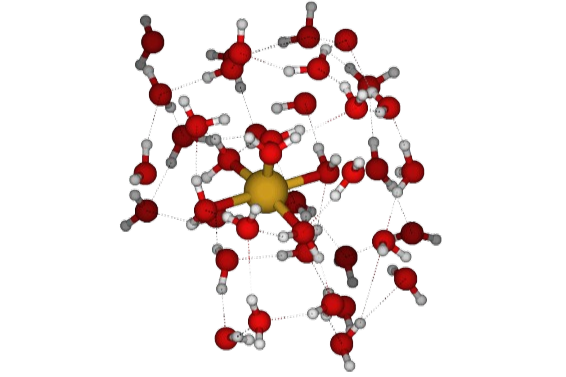
\includegraphics[width=\linewidth]{Imágenes/PC_40.png}
        \text{PC}
    \end{minipage}\hfill
    \begin{minipage}[b]{0.48\textwidth}
        \centering
        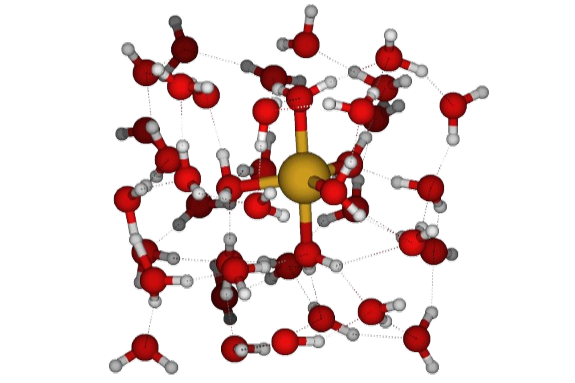
\includegraphics[width=\linewidth]{Imágenes/BT_40.png}
        \text{BT}
    \end{minipage}

    \vspace{0.4cm}

    % --- Fila 2: PT y OD en cúmulo de 40 ---
    \begin{minipage}[b]{0.48\textwidth}
        \centering
        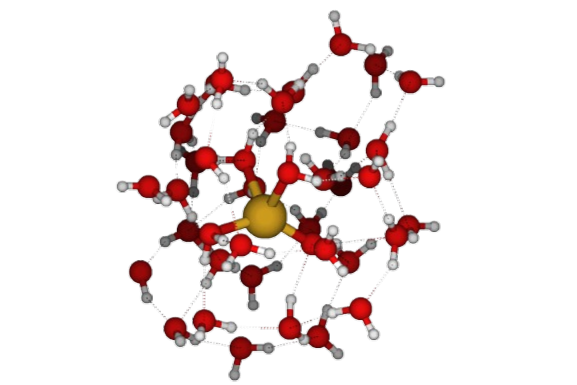
\includegraphics[width=\linewidth]{Imágenes/PT_40.png}
        \text{PT}
    \end{minipage}\hfill
    \begin{minipage}[b]{0.48\textwidth}
        \centering
        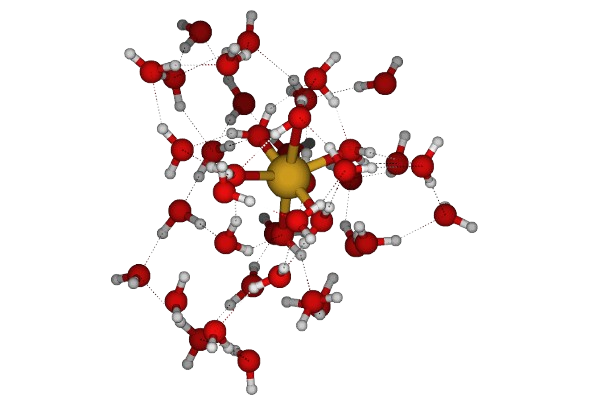
\includegraphics[width=\linewidth]{Imágenes/OD_40.png}
        \text{OD}
    \end{minipage}

    \vspace{0.4cm}

    % --- Fila 3: Las 4 geometrías aisladas ---
    \begin{minipage}[b]{0.23\textwidth}
        \centering
        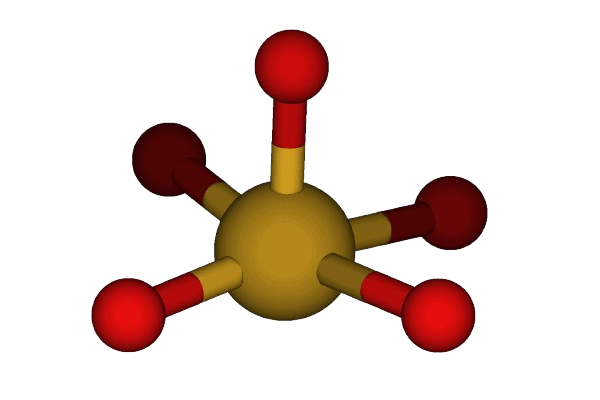
\includegraphics[width=\linewidth]{Imágenes/PC_aislada.png}
        \text{PC}
    \end{minipage}\hfill
    \begin{minipage}[b]{0.23\textwidth}
        \centering
        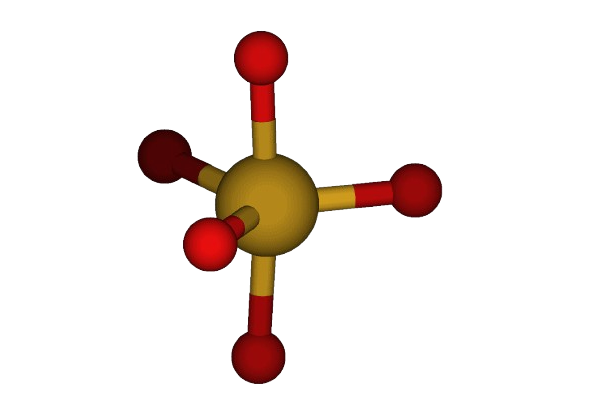
\includegraphics[width=\linewidth]{Imágenes/BT_aislada.png}
        \text{BT}
    \end{minipage}\hfill
    \begin{minipage}[b]{0.23\textwidth}
        \centering
        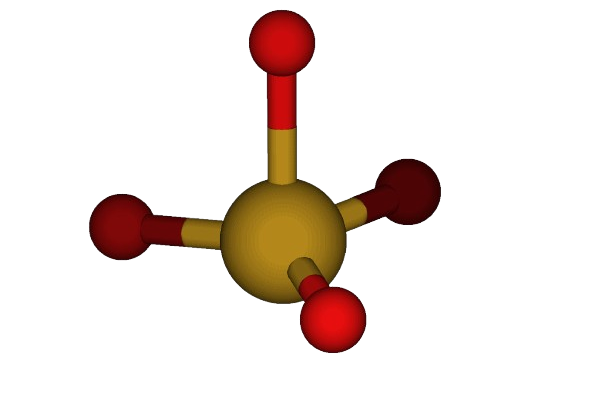
\includegraphics[width=\linewidth]{Imágenes/PT_aislada.png}
        \text{PT}
    \end{minipage}\hfill
    \begin{minipage}[b]{0.23\textwidth}
        \centering
        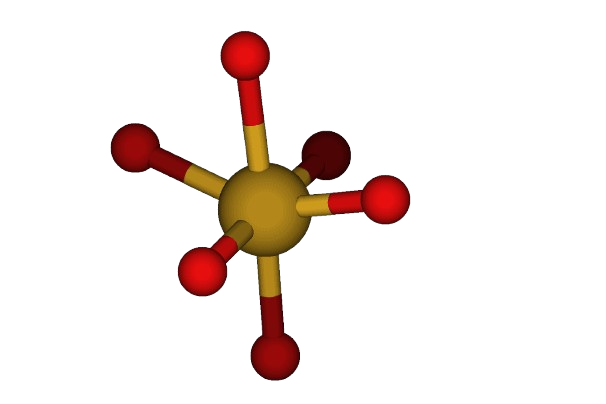
\includegraphics[width=\linewidth]{Imágenes/OD_aislada.png}
        \text{OD}
    \end{minipage}

    \caption[Geometrías representativas de la primera esfera, \ce{[Cu(H2O)_{40}]^{2+}}]{Geometrías representativas observadas en la primera esfera de
    coordinación del sistema \ce{[Cu(H2O)_{40}]^{2+}} extraídas de la simulación. Filas
    superior e intermedia: cada geometría representada en el cúmulo completo de 40 moléculas;
    fila inferior: primera esfera de coordinación aislada. Las geometrías predominantes son la
    \textbf{pirámide cuadrada} (PC), la \textbf{bipirámide trigonal} (BT)
    y la \textbf{pirámide trigonal} (PT), las cuales se intercambian de forma
    continua a lo largo de la dinámica. La geometría \textbf{octaédrica distorsionada} (OD)
    se incluye como referencia, pues su ocurrencia es considerablemente menor que la de las
    anteriores.}
    \label{fig:geom_repr_agua}
\end{figure}

Estas tres geometrías son consistentes con el perfil de la ADF y el histograma mostrado en la figura \ref{fig:nc_distribution_water}. El pico principal en $\theta \approx 87^\circ$ corresponde a los ángulos ecuatoriales de la pirámide cuadrada, que se encuentran ligeramente por debajo de los $90^\circ$ ideales; esta desviación se atribuye al movimiento térmico de las moléculas de solvente, que genera fluctuaciones importantes alrededor de cualquier ángulo de referencia ideal. El hombro que se extiende entre $\sim\!100^\circ$ y $\sim\!130^\circ$ incluye los ángulos ecuatorial axial de la pirámide cuadrada, en el intervalo de $100^\circ$--$110^\circ$, y los ángulos ecuatoriales de la bipirámide trigonal, cercanos a los $120^\circ$ esperados para esta geometría; el hecho de que esta región no presente un máximo claro indica que el sistema transita continuamente entre ambas estructuras, y que el movimiento térmico ensancha las distribuciones. Por último, la región de $145^\circ$--$152^\circ$ agrupa los ángulos que en un octaedro ideal serían de $180^\circ$, pero que aquí aparecen reducidos debido al movimiento térmico del sistema, lo que es consistente con la baja proporción de estructuras hexacoordinadas observada en la trayectoria.

\subsection*{Termalización y estabilidad energética}

A partir de este punto, la discusión se centrará en el análisis de la trayectoria correspondiente a la réplica A (ver tabla \ref{tab:replicas_md}), cuya propagación se extendió por un periodo de 20 ps, intervalo que constituye el tiempo de muestreo recomendado para el presente sistema y que garantiza un colectivo estadísticamente suficiente para la evaluación de propiedades dinámicas
y fenómenos que demandan un tratamiento temporal continuo.

Previo al análisis de las propiedades, resultó necesario evaluar el periodo de termalización del sistema. Para ello, se desarrolló un programa en Python orientado a la extracción de las energías totales del cúmulo en cada paso de integración. A partir de estos datos, se calculó la evolución temporal de la energía de enlace por molécula de agua empleando la ecuación \ref{eq:energia_enlace}. La monitorización de esta magnitud es fundamental para verificar la suficiencia del periodo de termalización y descartar la presencia de derivas energéticas a lo largo de la simulación. El perfil resultante se muestra en la Figura~\ref{fig:energy_water}.

% --- Evolución de la energía ---
\begin{figure}[htbp]
    \centering
    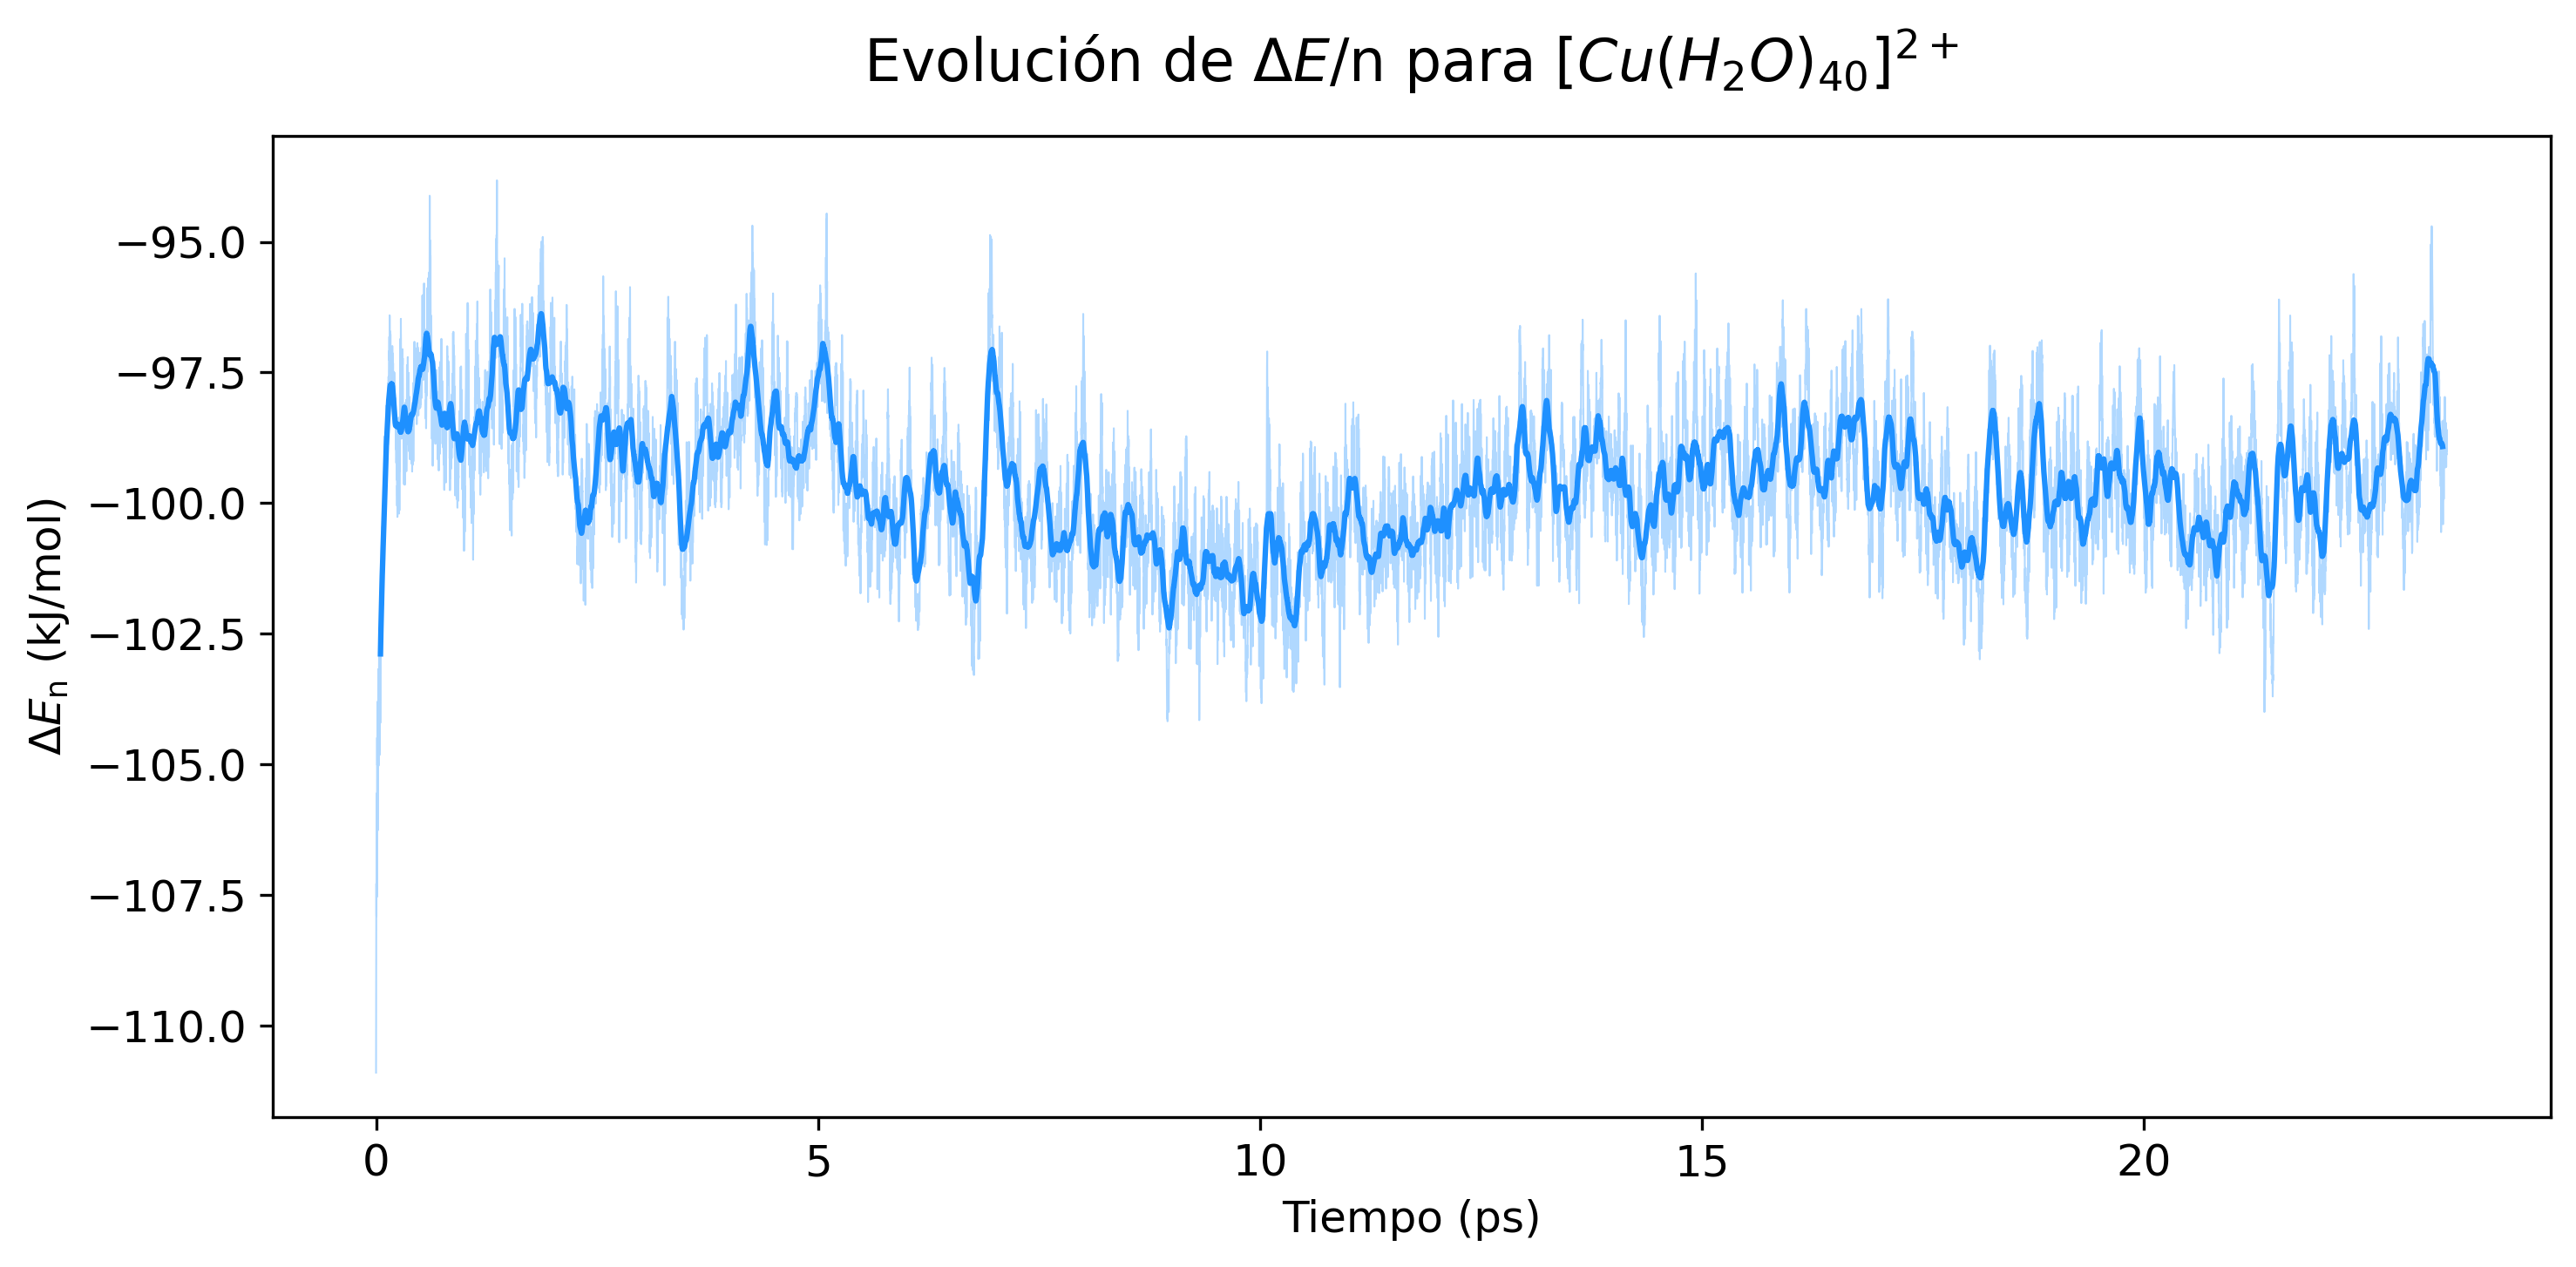
\includegraphics[width=0.95\textwidth]{Imágenes/md_energy_water.png}
    \caption[Evolución de la diferencia de potencial por molécula para \ce{[Cu(H2O)40]^{2+}}]{Evolución de la diferencia de potencial por molécula de agua durante la simulación de dinámica molecular para el sistema \ce{[Cu(H2O)40]^{2+}}.}
    \label{fig:energy_water}
\end{figure}

El perfil termodinámico evidencia que el periodo de termalización de 3 ps es suficiente para alcanzar el equilibrio: la energía parte de un valor inicial de $-110.9$ kJ/mol, correspondiente a la configuración optimizada del cúmulo de partida, y rápidamente adopta un comportamiento fluctuante pero esperado en una simulación de dinámica molecular.
El análisis estadístico del periodo de post termalización (a partir de los 3 ps) arroja una diferencia de energía potencial de $\langle \Delta E/n \rangle = -99.9 \pm 1.3$ kJ/mol por molécula de agua, con fluctuaciones de amplitud $\sim 9.5$ kJ/mol.

\subsection*{Eventos de intercambio}

Para identificar los eventos de intercambio entre la primera y la segunda esfera de coordinación, se realizó un seguimiento temporal de las distancias \ce{Cu^{2+}}-- O para todos los oxígenos de la nanogota, calculando en cada paso temporal la distancia respecto al ion central. El radio de corte empleado para delimitar la primera esfera es el mismo utilizado en el cálculo del número de coordinación ($r_{corte} = 2.833$~\AA).
En total, 19 de los 40 oxígenos residieron en la primera esfera de coordinación durante algún intervalo de la trayectoria. La Figura \ref{fig:distancias_panoramica_agua} muestra la evolución temporal de las distancias para solo 8 de estas moléculas, seleccionadas por ser protagonistas de los eventos de intercambio identificados; las moléculas restantes que no cruzaron el radio de corte se omiten por claridad visual. La notación O$_i$ es utilizada para control interno del programa de análisis.

\begin{figure}[htbp]
    \centering
    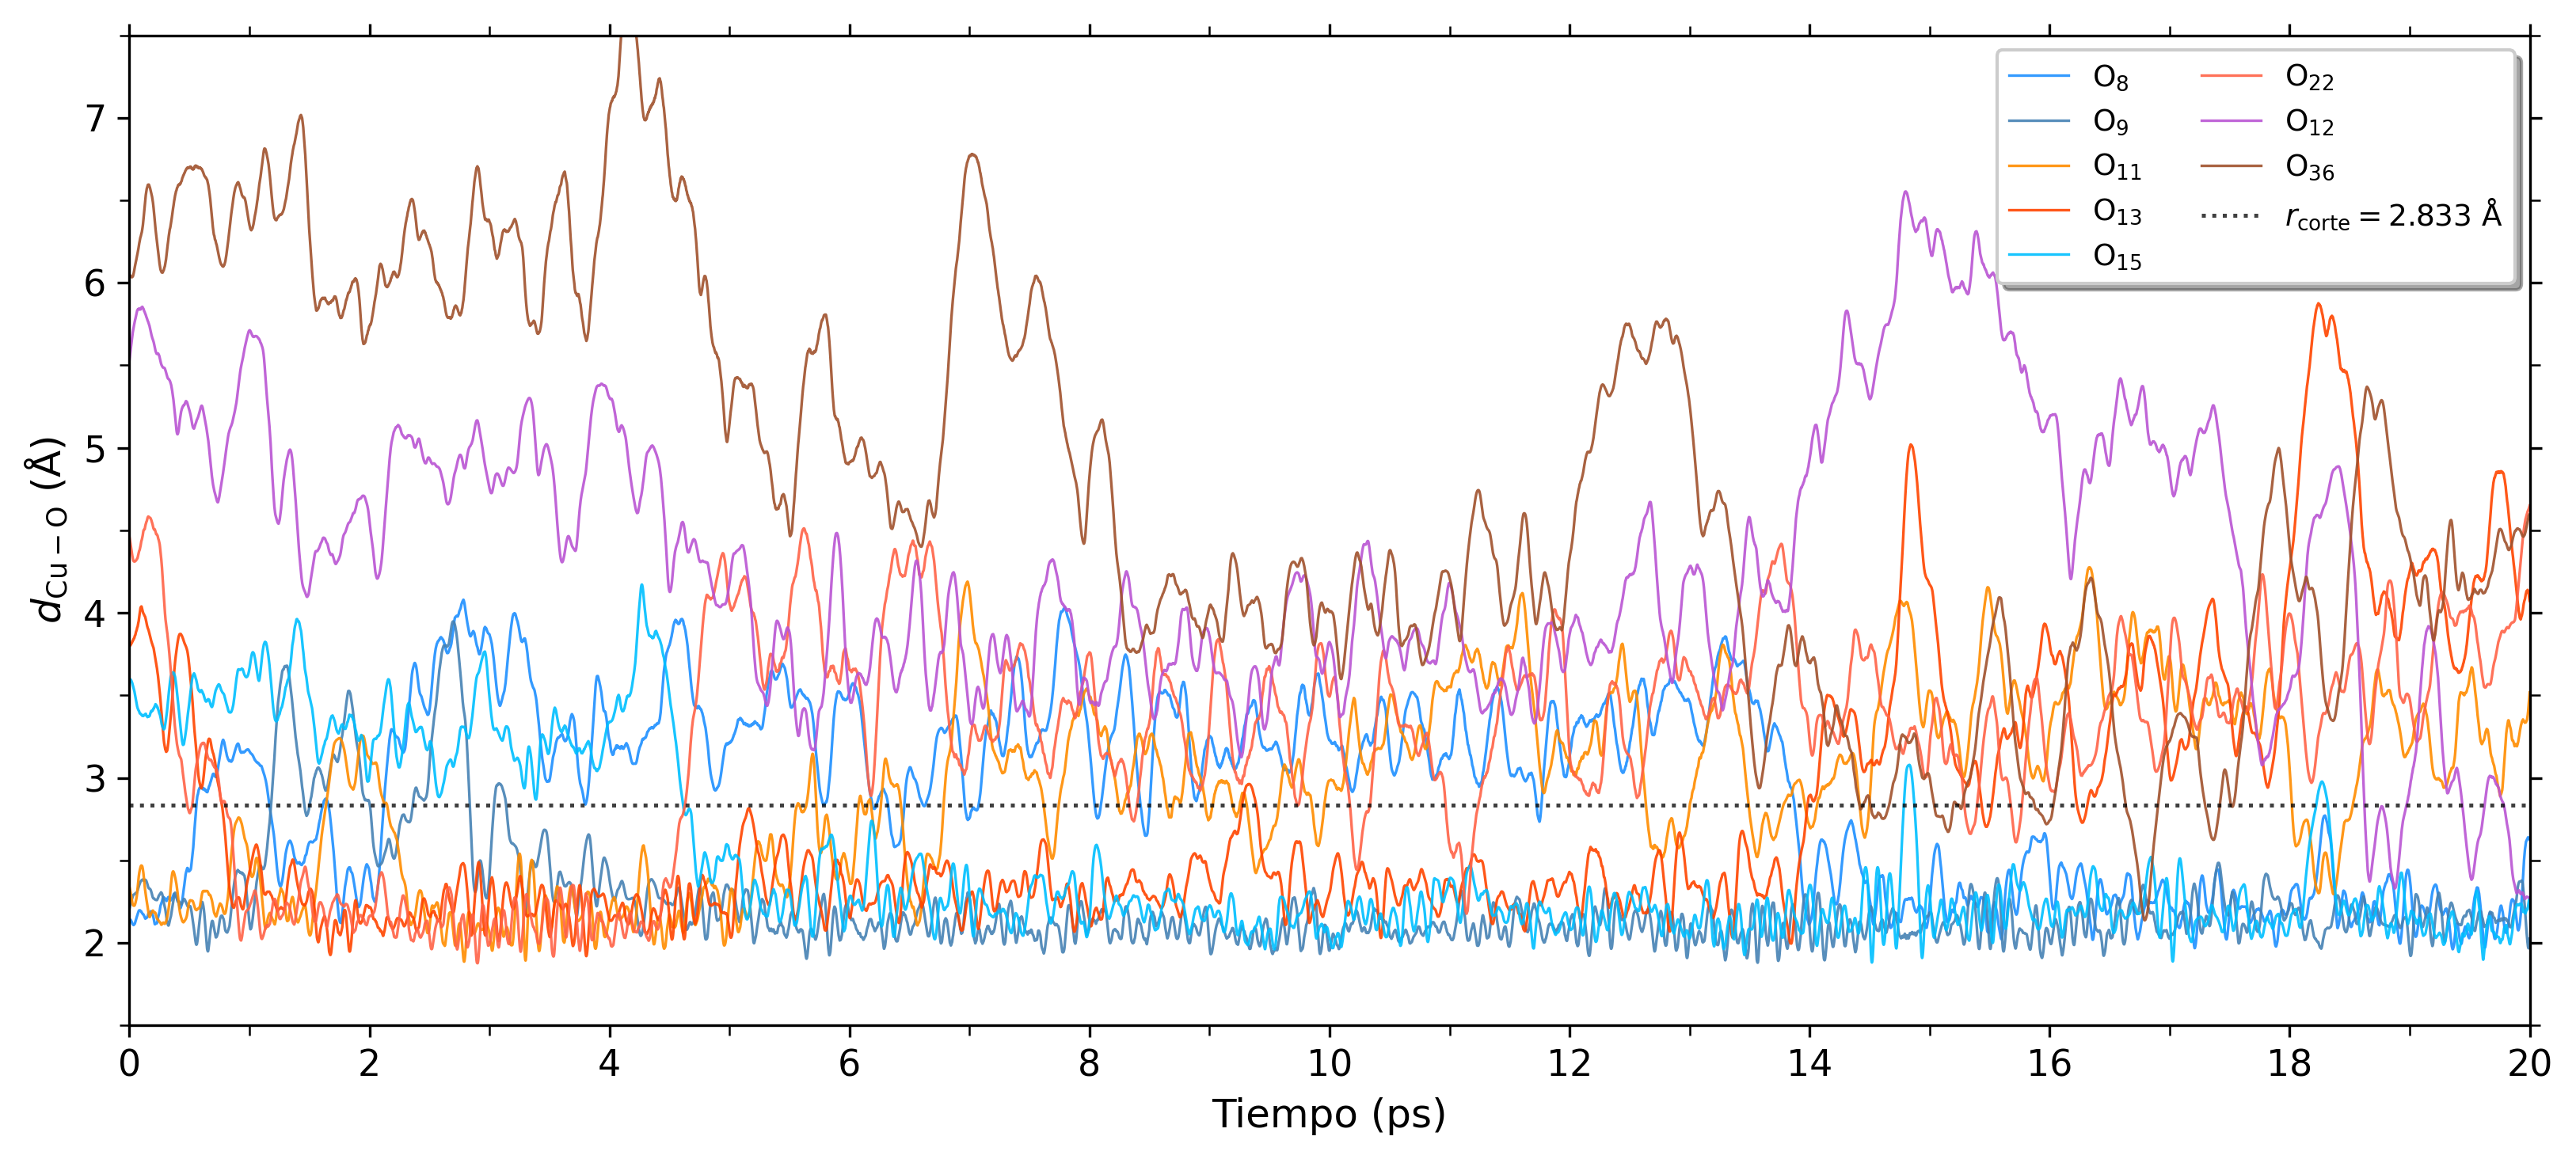
\includegraphics[width=0.95\textwidth]{Imágenes/distancias_panoramica.png}
    \caption[Evolución de distancias \ce{Cu^{2+}}--O para \ce{[Cu(H2O)_{40}]^{2+}}]{
        Evolución temporal de las distancias \ce{Cu^{2+}}--O para las 8 moléculas
        de agua que presentaron los eventos de intercambio o trayectorias de mayor
        interés dinámico durante la réplica A del sistema \ce{[Cu(H2O)_{40}]^{2+}}.
        La línea punteada indica el radio de corte $r = 2.833$~\AA{} que
        delimita la primera esfera de coordinación.}
    \label{fig:distancias_panoramica_agua}
\end{figure}

A lo largo de los 20 ps analizados se identificaron dos eventos de intercambio y una trayectoria de especial interés dinámico, que se describen a continuación en las figuras \ref{fig:distancias_O8_O13}, \ref{fig:distancias_O15_O22} y \ref{fig:distancias_O12}.

\begin{figure}[H]
    \centering
    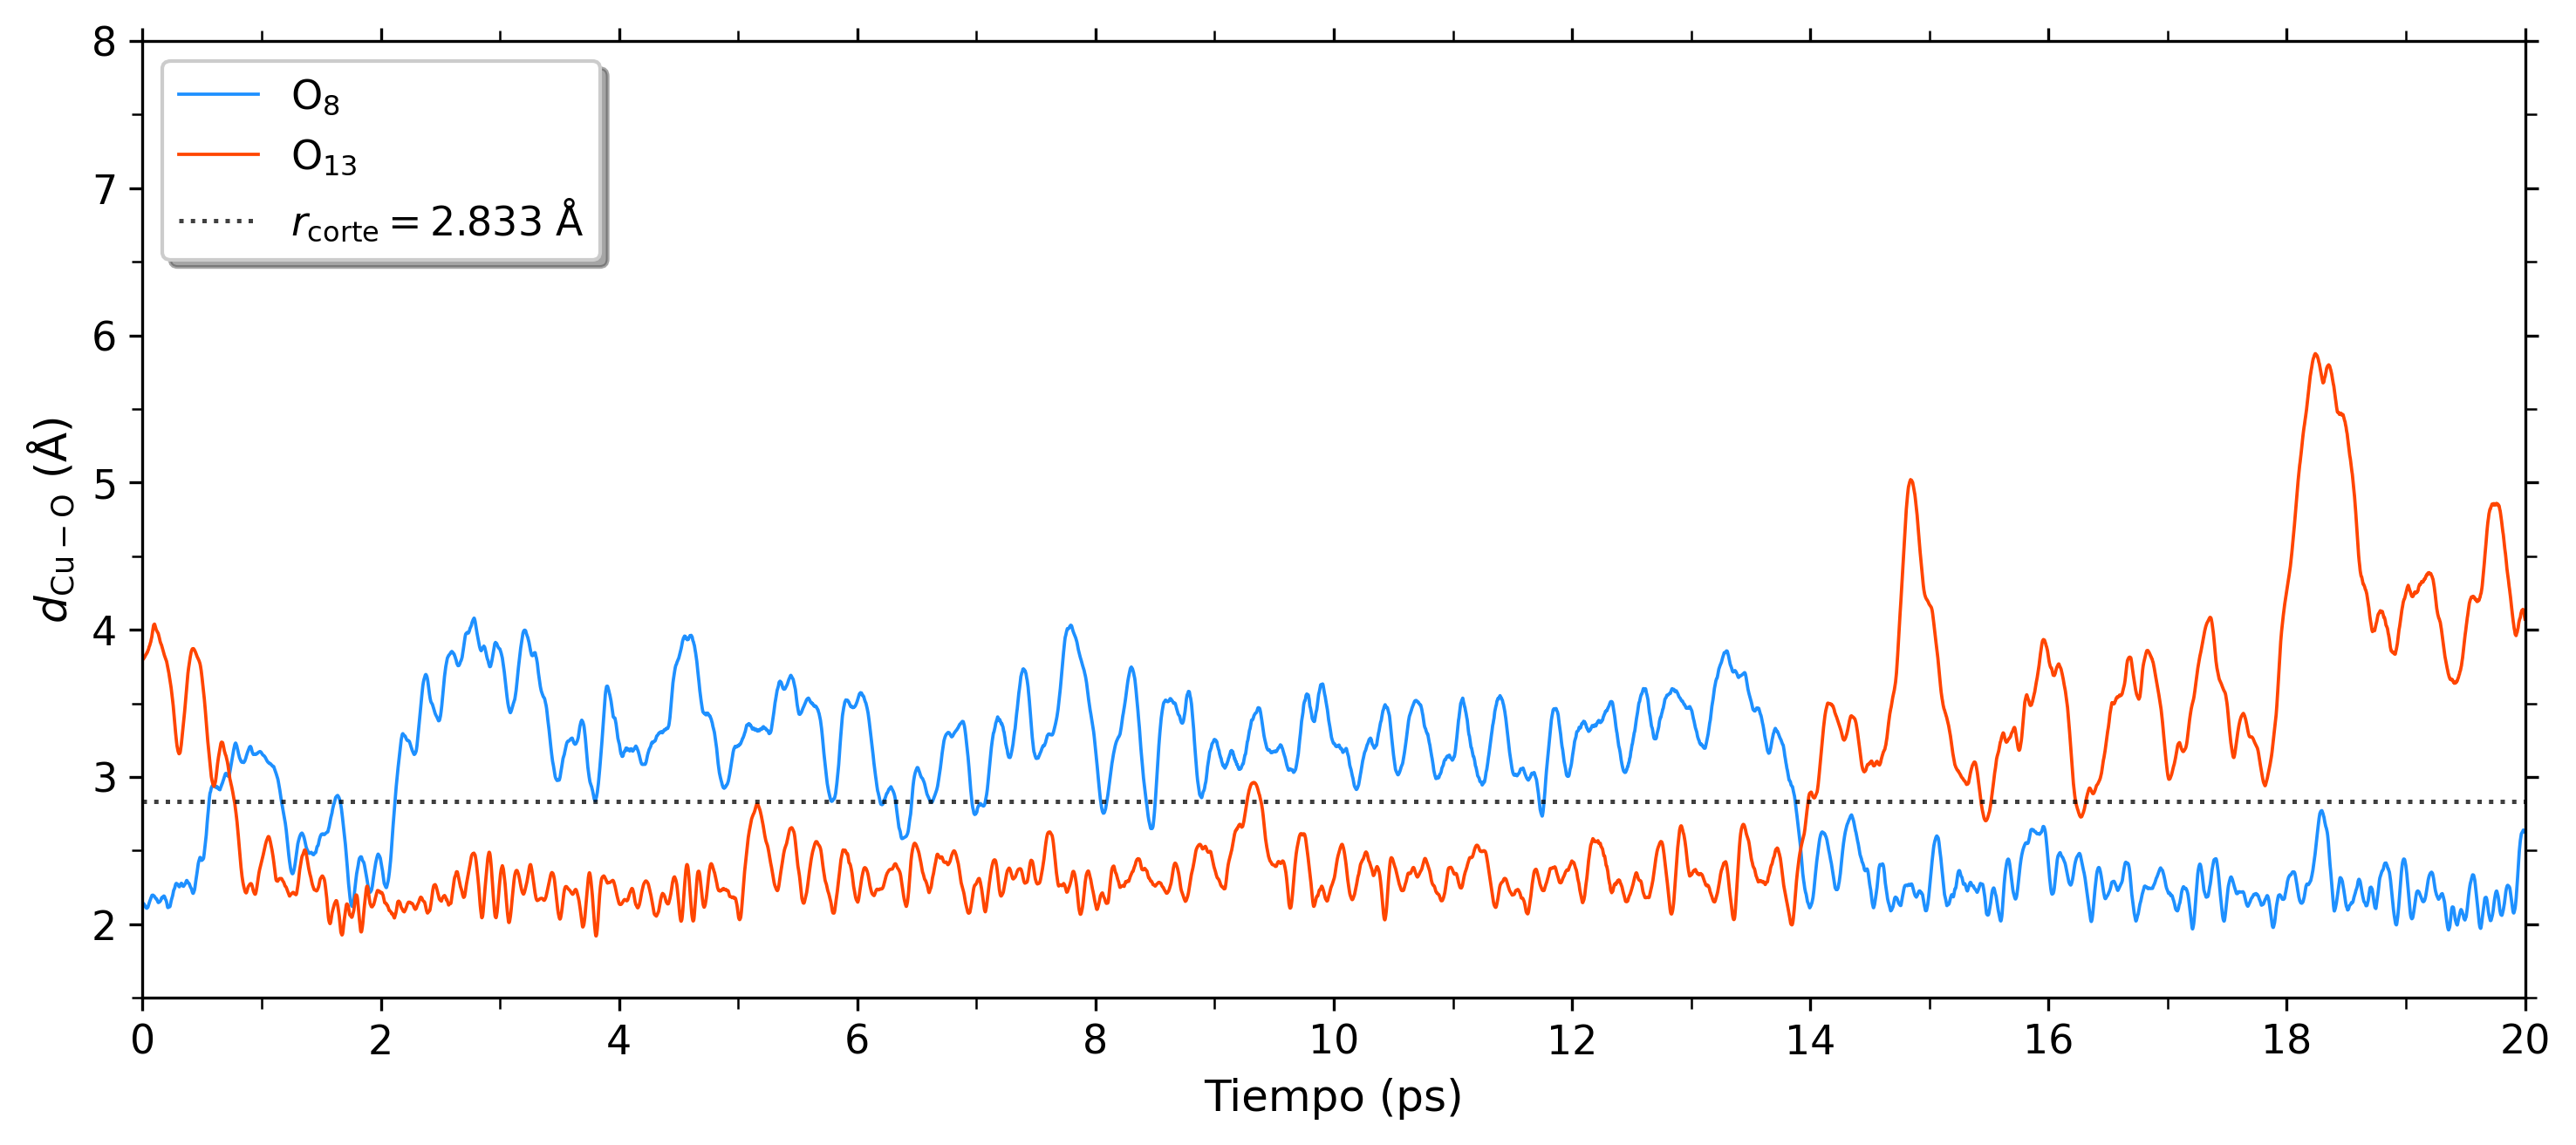
\includegraphics[width=0.85\textwidth]{Imágenes/distancias_O8_O13.png}
    \caption[Evento de intercambio de ligandos O$_8$ $\leftrightarrow$ O$_{13}$]{Seguimiento temporal de las distancias \ce{Cu^{2+}}--O$_8$ y \ce{Cu^{2+}}--O$_{13}$ revela un evento de intercambio. El cruce ocurre en torno a $t \approx 14$ ps, cuando ambas moléculas se aproximan al radio de corte de manera simultánea.}
    \label{fig:distancias_O8_O13}
\end{figure}

\begin{figure}[H]
    \centering
    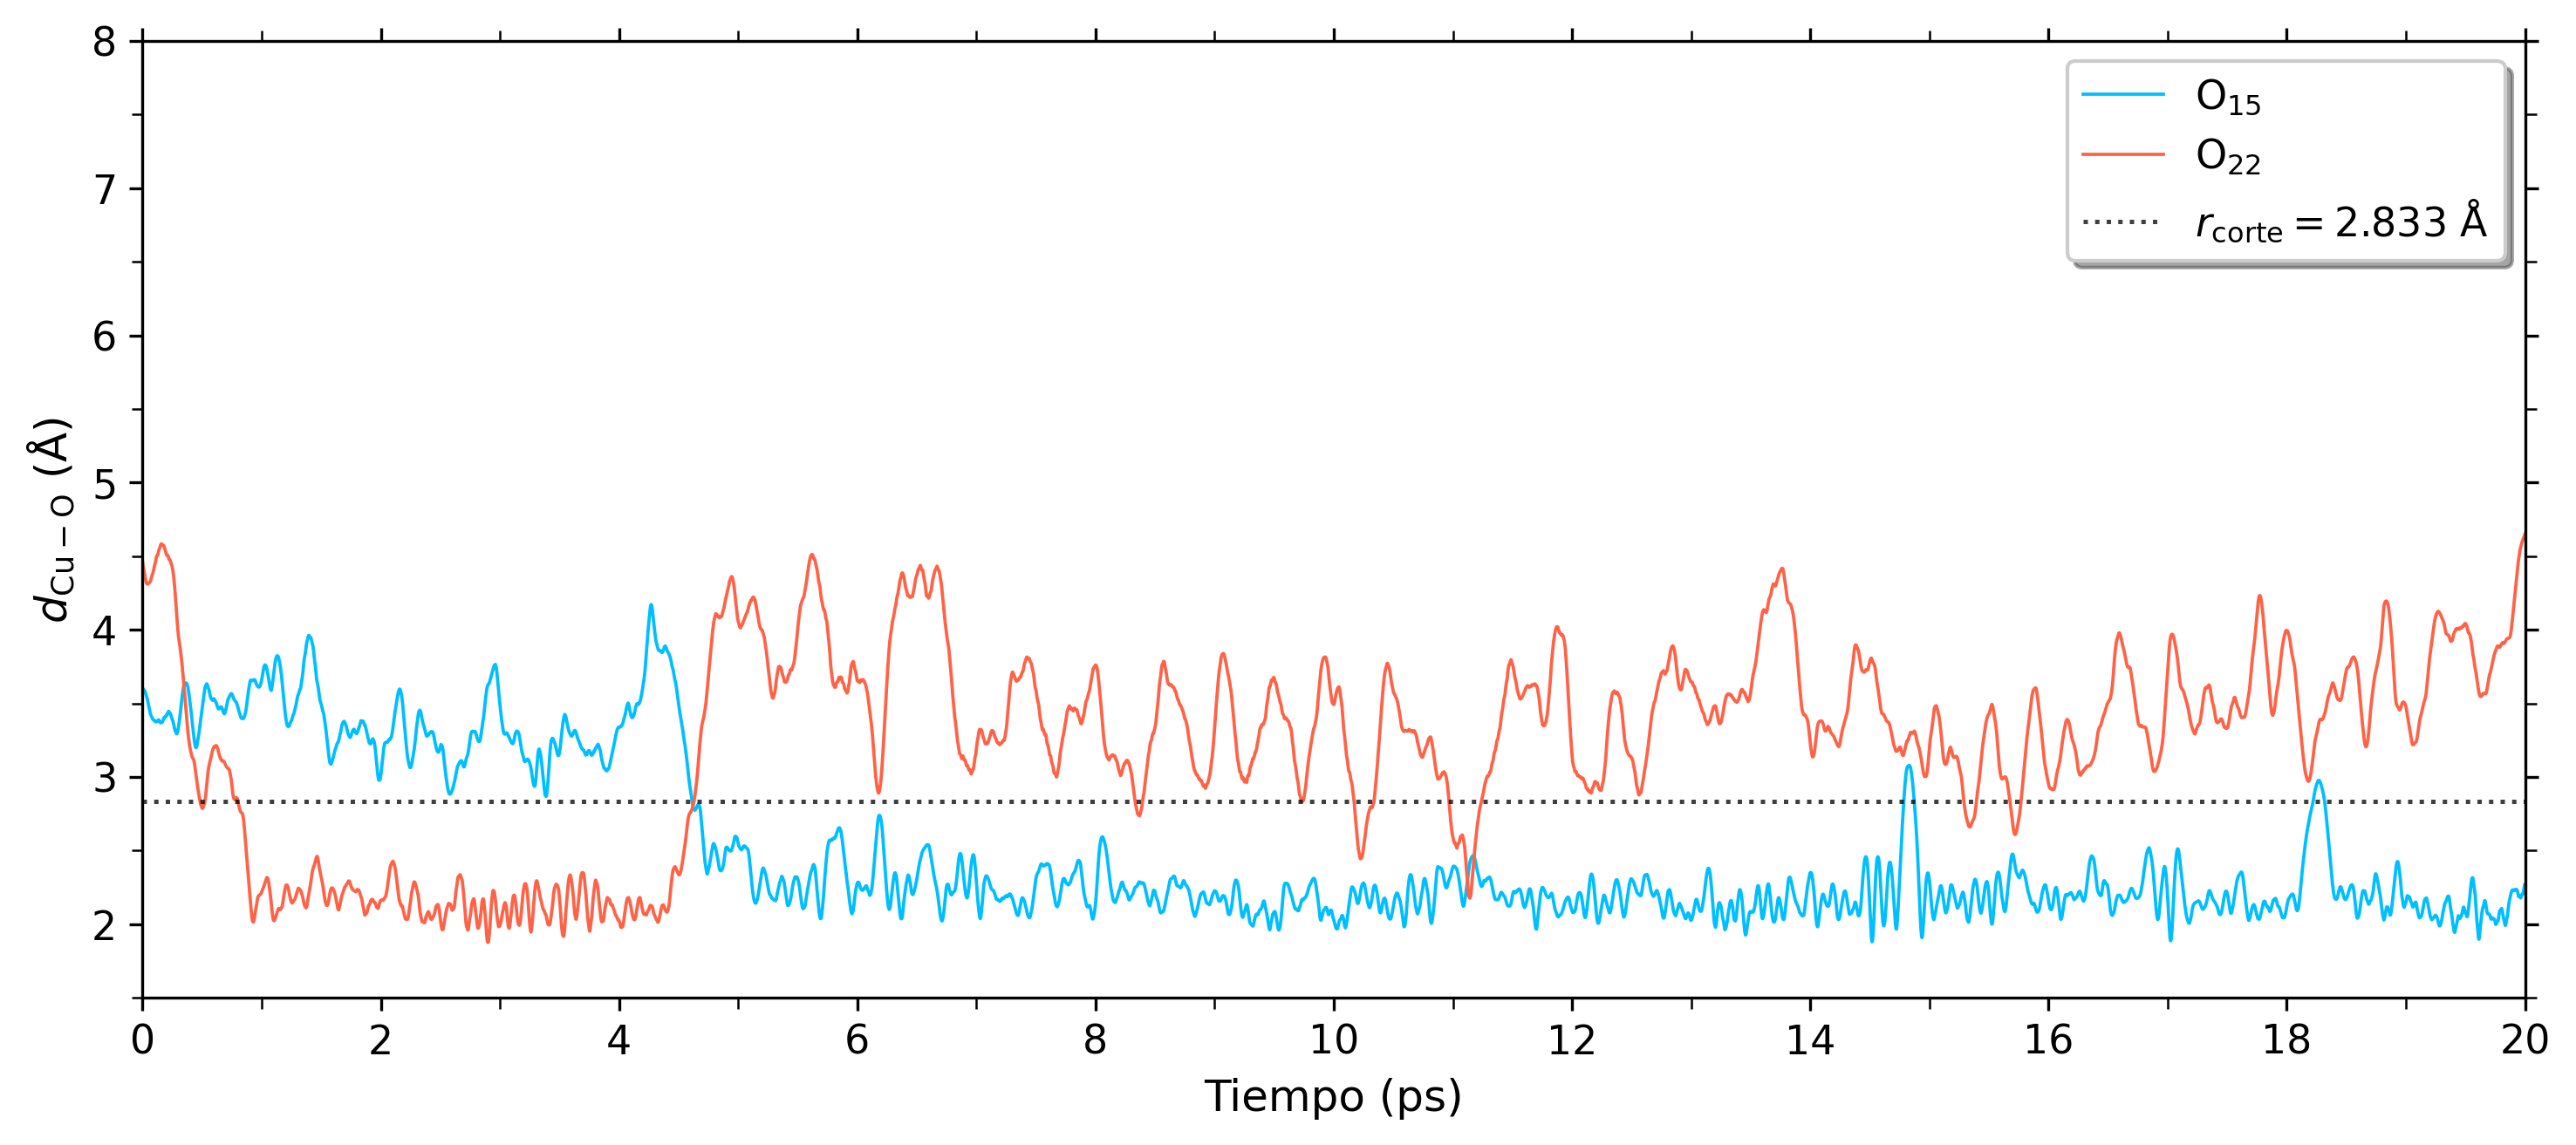
\includegraphics[width=0.95\textwidth]{Imágenes/distancias_O15_O22.png}
    \caption[Evento de intercambio de ligandos O$_{15}$ $\leftrightarrow$ O$_{22}$]{
        Evento de intercambio entre O$_{15}$ y O$_{22}$. La transición se produce en $t \approx 4.6$~ps. Tras el intercambio, O$_{22}$ no regresa a la primera esfera incluso cuando llega a cruzar momentáneamente el radio de corte.}
    \label{fig:distancias_O15_O22}
\end{figure}

La trayectoria del oxígeno O$_{12}$ constituye un ejemplo ilustrativo de la información que puede extraerse del análisis de distancias. Al inicio de la simulación (post termalización), O$_{12}$ se encuentra dentro de la segunda esfera de coordinación y se mantiene dentro hasta $t \approx 14.2$~ps. En ese punto, O$_{12}$ se aleja brevemente, pero regresa y a partir de $t \approx 18.6$ ps logra colocarse dentro de la primer esfera.

\begin{figure}[htbp]
    \centering
    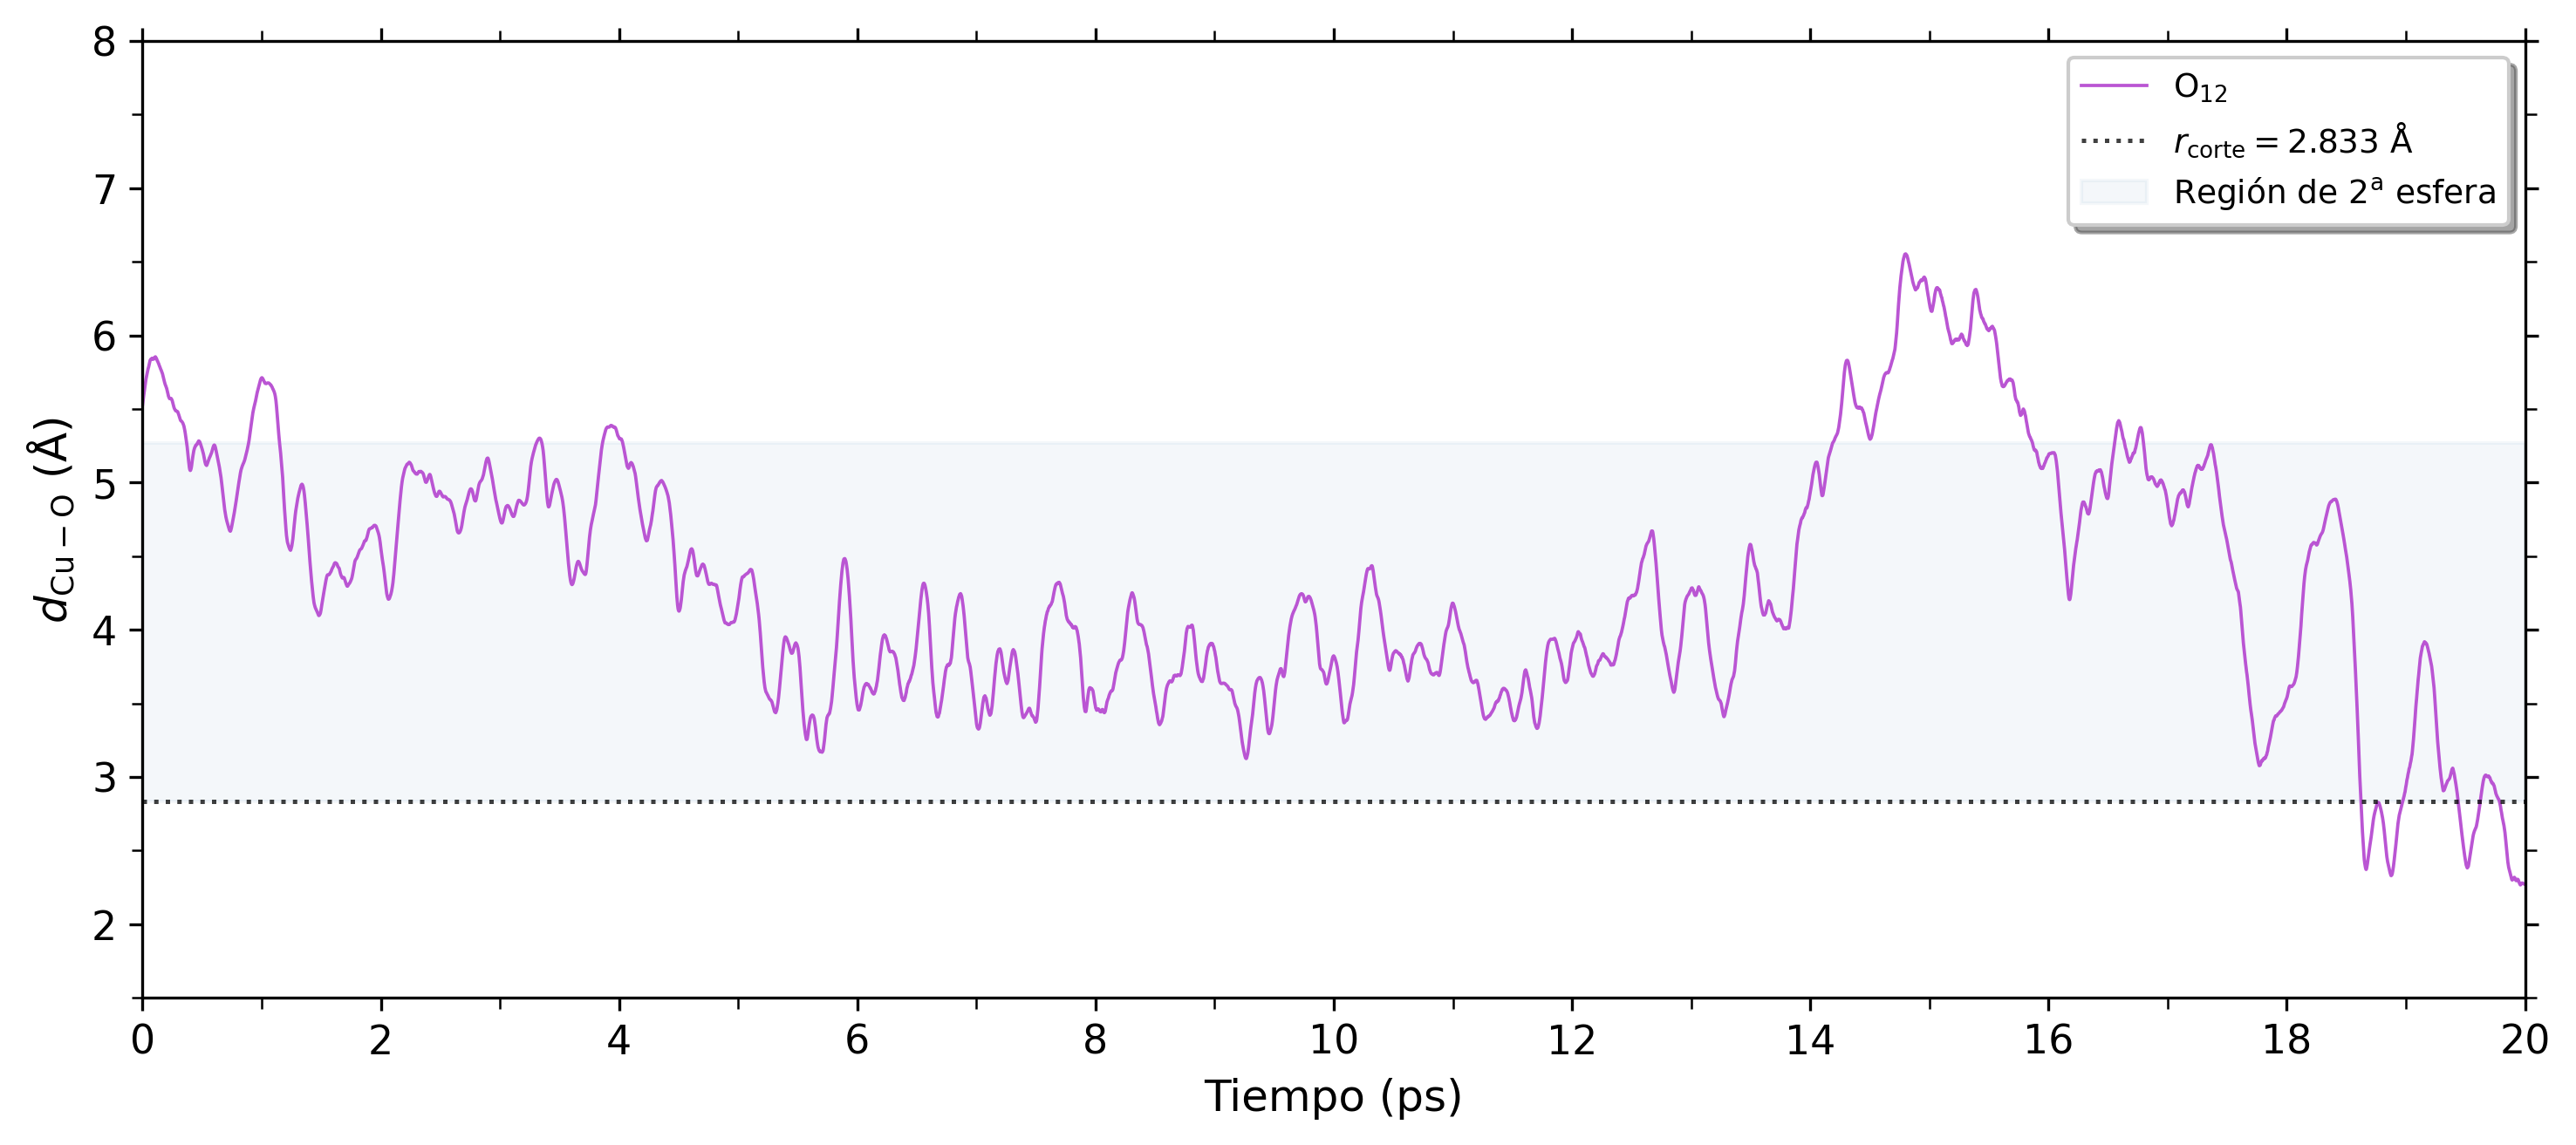
\includegraphics[width=0.95\textwidth]{Imágenes/distancias_O12.png}
    \caption[Trayectoria dinámica de O$_{12}$]{
        Evolución temporal de la distancia \ce{Cu^{2+}}--O$_{12}$, que ilustra una trayectoria dinámica de interés. O$_{12}$}
    \label{fig:distancias_O12}
\end{figure}

Estudios teóricos y experimentales, han estimado tiempos de residencia del orden de $\sim$ 100 - 200 ps \cite{Wa-2013-02, Wa-2009-02}, valores que deben interpretarse con cautela dada la sensibilidad de esta cantidad al nivel de teoría empleado y de las limitaciones experimentales propias de la época. En este contexto, el hecho de que en una trayectoria BOMD de tan solo $\sim$20 ps hayan podido observarse eventos de intercambio de ligandos sugiere que el tiempo de residencia real podría ser sensiblemente menor que los valores previamente reportados, situándose posiblemente en el orden de las decenas de picosegundos. Si bien la longitud de la trayectoria no permite un cálculo estadístico riguroso de $\tau$, los eventos capturados son cualitativamente consistentes con la labilidad característica del \ce{Cu^{2+}} en agua.

\section{Cúmulo \ce{[Cu(CH3OH)40]^{2+}}}

\subsection*{Función de distribución radial y solvatación en primera esfera}

En contraste con la solvatación del \ce{Cu^{2+}} en agua, el caso del metanol ha sido considerablemente menos abordado por la comunidad científica, como se discute en el capítulo de Antecedentes. En particular, no existe hasta la fecha ningún estudio de dinámica molecular para este sistema, por lo que el presente trabajo constituye la primera caracterización estructural y dinámica obtenida mediante esta técnica.
El análisis sigue la misma metodología descrita para el cúmulo de agua y, con el fin de evitar redundancias, se apoyará en la comparación directa con ese sistema. La RDF obtenida se muestra en la Figura \ref{fig:rdf_metanol} y los parámetros estructurales se resumen en la Tabla \ref{tab:rdf_comparativa}.

% --- RDF METANOL ---
\begin{figure}[htbp]
    \centering
    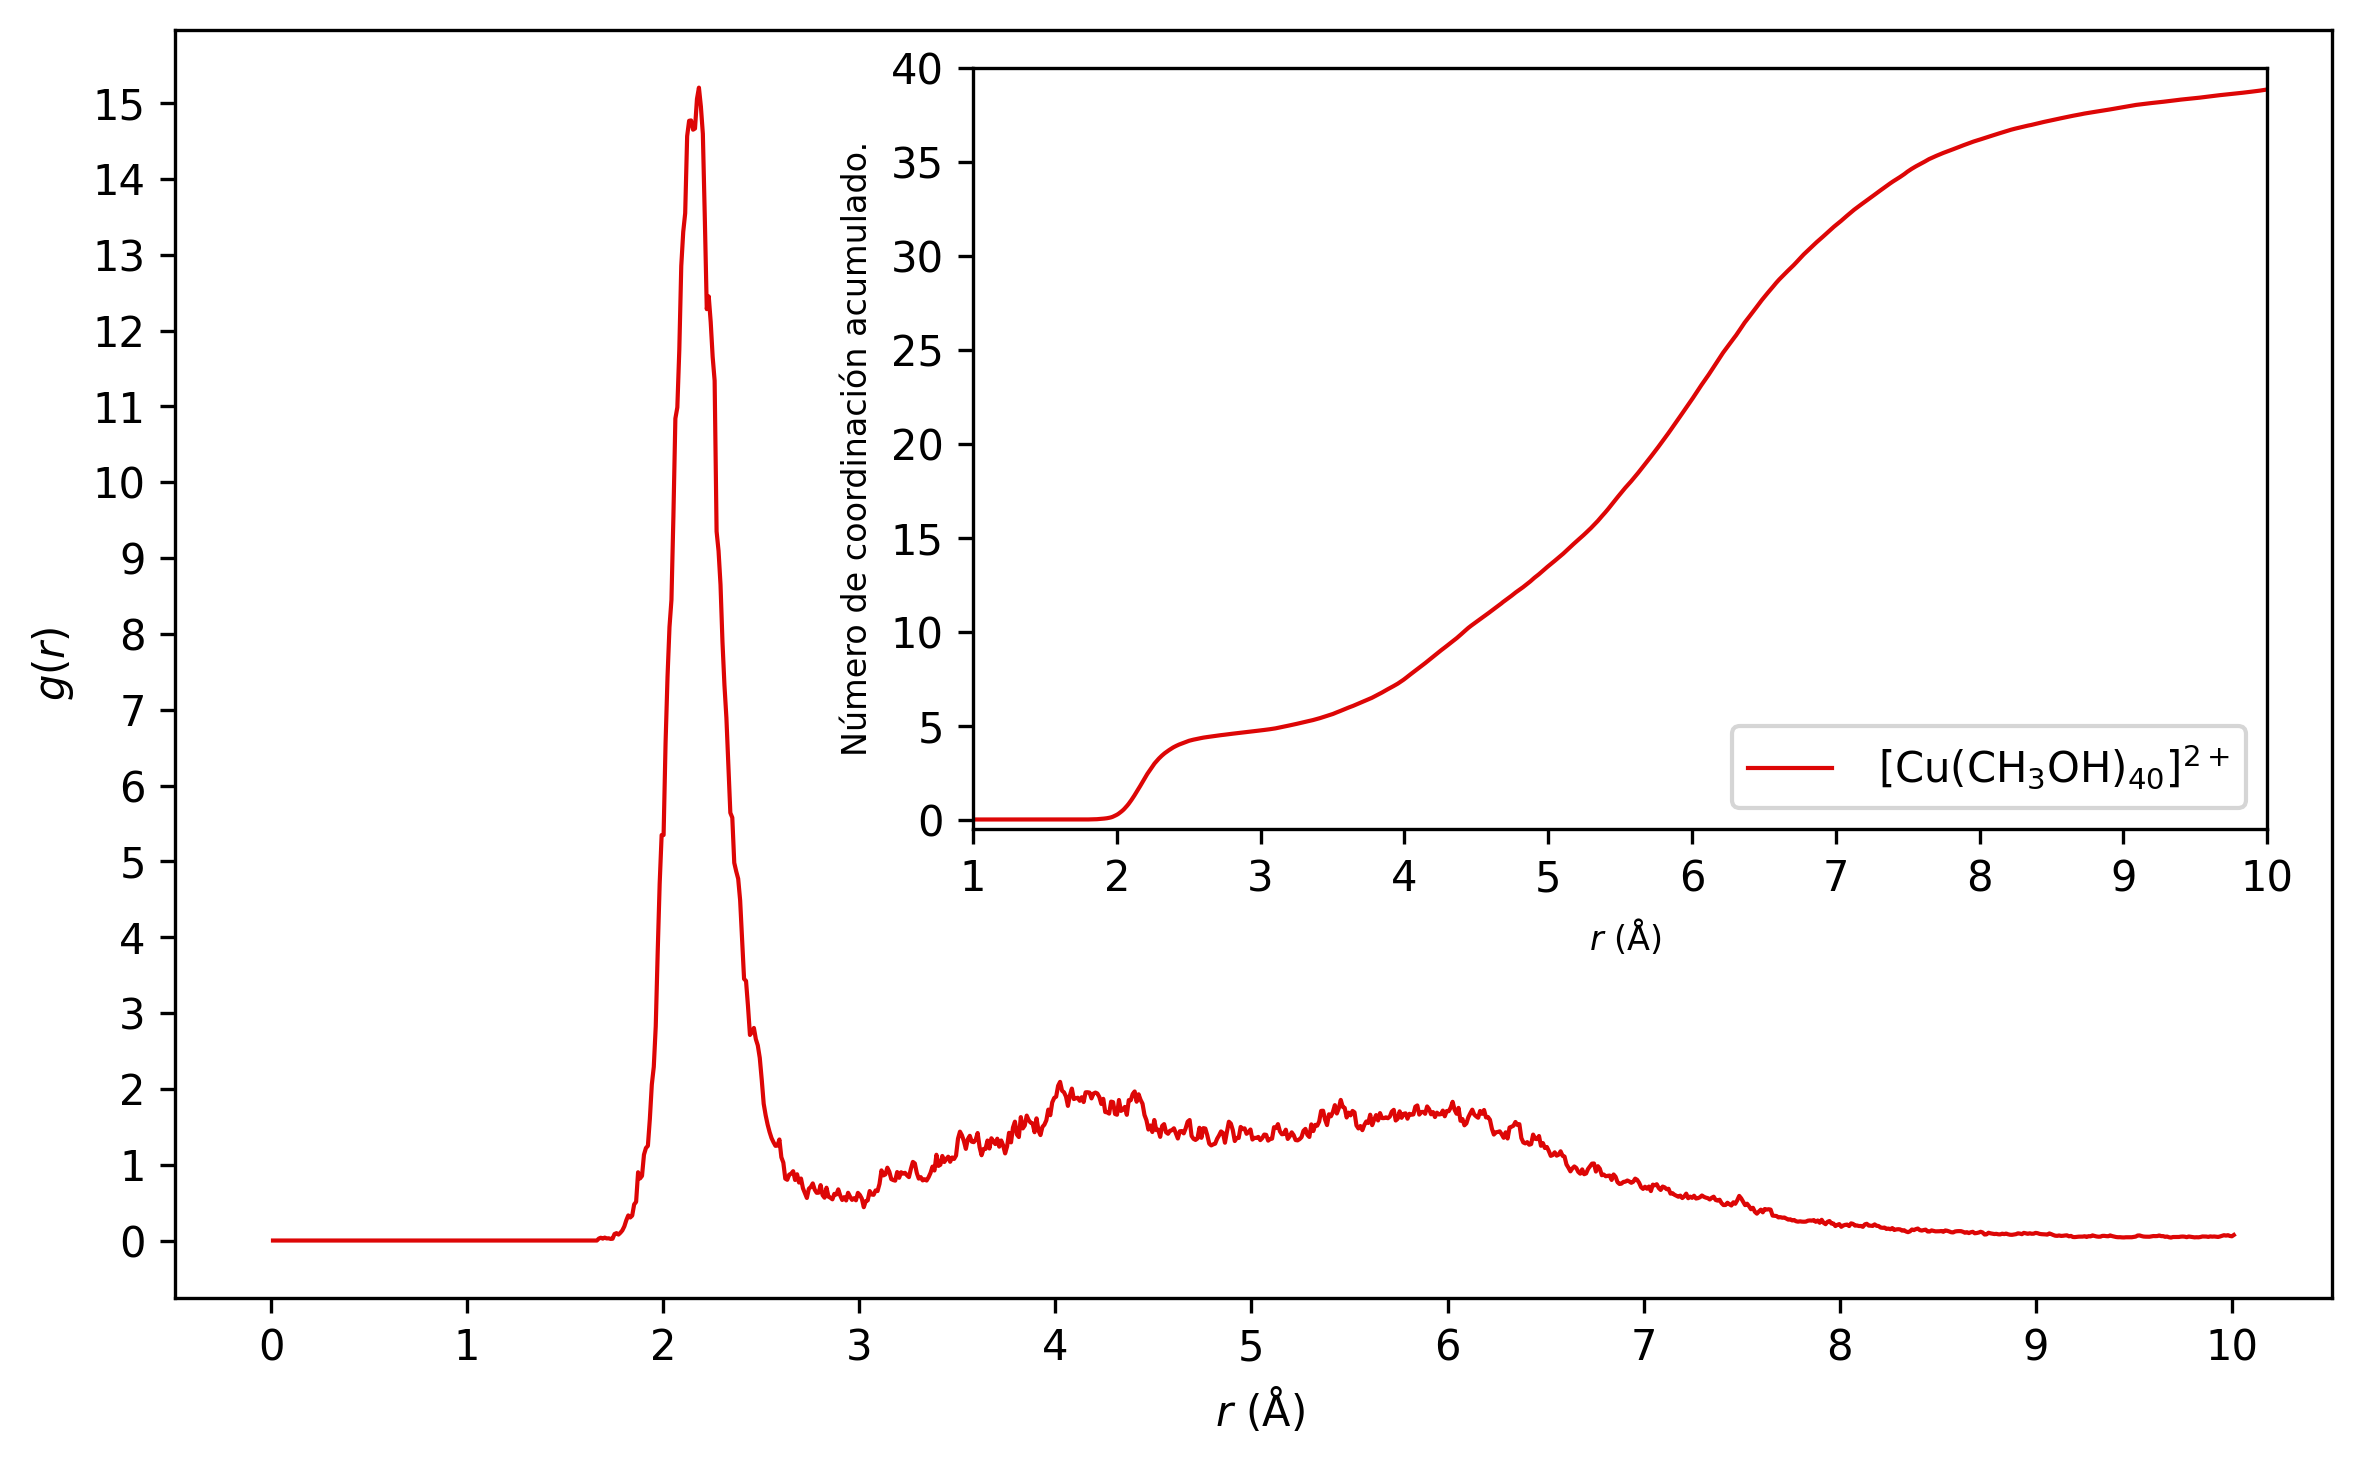
\includegraphics[width=0.95\textwidth]{Imágenes/RDF-OUTPUT-HISTOGRAMA-METANOL.png}
    \caption[RDF para cúmulo \ce{[Cu(CH3OH)40]^{2+}}]{Función de distribución radial (RDF) obtenida para el sistema \ce{[Cu(CH3OH)40]^{2+}} a partir de la simulación de dinámica molecular.}
    \label{fig:rdf_metanol}
\end{figure}

\begin{table}[htbp]
    \centering
    \caption{Comparación de los parámetros estructurales de la RDF Cu--O obtenidos para los sistemas \ce{[Cu(H2O)40]^{2+}} y \ce{[Cu(CH3OH)40]^{2+}}.}
    \label{tab:rdf_comparativa}
    \begin{tabularx}{\textwidth}{>{\raggedright\arraybackslash}p{0.28\textwidth} >{\centering\arraybackslash}p{0.15\textwidth} >{\centering\arraybackslash}p{0.12\textwidth} >{\centering\arraybackslash}p{0.15\textwidth} >{\centering\arraybackslash}p{0.12\textwidth}} 
        \hline
        \textbf{Parámetro} 
            & \multicolumn{2}{c}{\ce{[Cu(H2O)40]^{2+}}} 
            & \multicolumn{2}{c}{\ce{[Cu(CH3OH)40]^{2+}}} \\
            & $r$ (\AA) & $g(r)$ & $r$ (\AA) & $g(r)$ \\
            \hline
            1\textsuperscript{er} máximo  & 2.182 & 6.339 & 2.182 & 15.199 \\
            1\textsuperscript{er} mínimo & 2.833 & 0.537 & 3.023 & 0.439  \\
            2\textsuperscript{do} máximo  & 4.014 & 1.820 & 4.024 & 2.092  \\
            3\textsuperscript{er} máximo  & ---   & ---   & 5.456 & 1.854  \\
            \hline
            NC ($r_\text{corte}$) & \multicolumn{2}{c}{4.73 ($r = 2.833$~\AA)} & \multicolumn{2}{c}{4.77 ($r = 3.23$~\AA)} \\
        \hline
    \end{tabularx}
\end{table}

El primer máximo presenta una altura notablemente mayor que en agua, lo cual no refleja una primera esfera más poblada sino un efecto de normalización: el metanol tiene una densidad numérica aproximadamente 2.26 veces menor que el agua, por lo que la misma cantidad de moléculas coordinadas representa una perturbación local proporcionalmente mayor. La posición del máximo, en cambio, es idéntica en ambos sistemas (2.182~\AA), pues la distancia \ce{Cu-O} está dominada por la interacción ion--dipolo directa entre el \ce{Cu^{2+}} y el oxígeno donador, independientemente del resto de la molécula de disolvente.

Lo que sí cambia es la organización de las esferas de coordinación. El primer mínimo se desplaza a 3.023~\AA, consecuencia directa del mayor volumen estérico del metanol: las moléculas no pueden comprimirse entre sí tan eficientemente en la zona de transición entre esferas. Al igual que en el agua, el valor $g(r) > 0$ en este mínimo es evidencia de la ocurrencia de eventos de intercambio de ligandos durante la dinámica.

La segunda esfera se manifiesta como un pico ancho en el intervalo $r \in [3.79,\,4.90]$~\AA, con un máximo local en $(r,\,g(r)) = (4.024\,,\,2.092)$ (muy similar al encontrado en el cúmulo de agua). A diferencia de ese sistema, $g(r)$ no decae limpiamente tras este máximo sino que permanece elevada hasta $r \approx 6.6$~\AA, sin que el muestreo estadístico disponible permita interpretar la estructura residual en esa región como una esfera de solvatación adicional.

El número de coordinación acumulado $n(r)$ confirma esta interpretación. En la región del primer mínimo ($r = 3.023$~\AA) se aprecia una meseta con $n = 4.77$, consistente con la dinámica de coordinación variable entre NC\,=\,4 y NC\,=\,5 discutida para el agua. Más allá de este punto, $n(r)$ crece de forma ininterrumpida y sin exhibir ninguna inflexión apreciable en la zona del segundo pico, lo que descarta un límite superior definido para la segunda esfera de coordinación. El máximo local en $r \approx 5.46$~\AA{} en la RDF no corresponde, por tanto, a la presencia de una tercera esfera de solvatación estructurada. El descenso parcial de $g(r)$ en $r \approx 4.79$~\AA{} podría atribuirse al cascarón que forman los grupos metilo de las moléculas de la segunda esfera, cuyos oxígenos coordinan hacia el \ce{Cu^{2+}} dejando los metilos orientados hacia afuera: esta capa hidrofóbica reduciría localmente la probabilidad de encontrar oxígenos adicionales antes de que aparezcan las moléculas de capas más externas en $r \approx 5.46$~\AA.

Adicionalmente, se muestra el histograma del número de coordinación a lo largo de la trayectoria, construido con el mismo procedimiento descrito para el sistema acuoso. Los  resultados se muestran en la figura \ref{fig:nc_distribution_methanol}.

\begin{figure}[H]
    \centering
    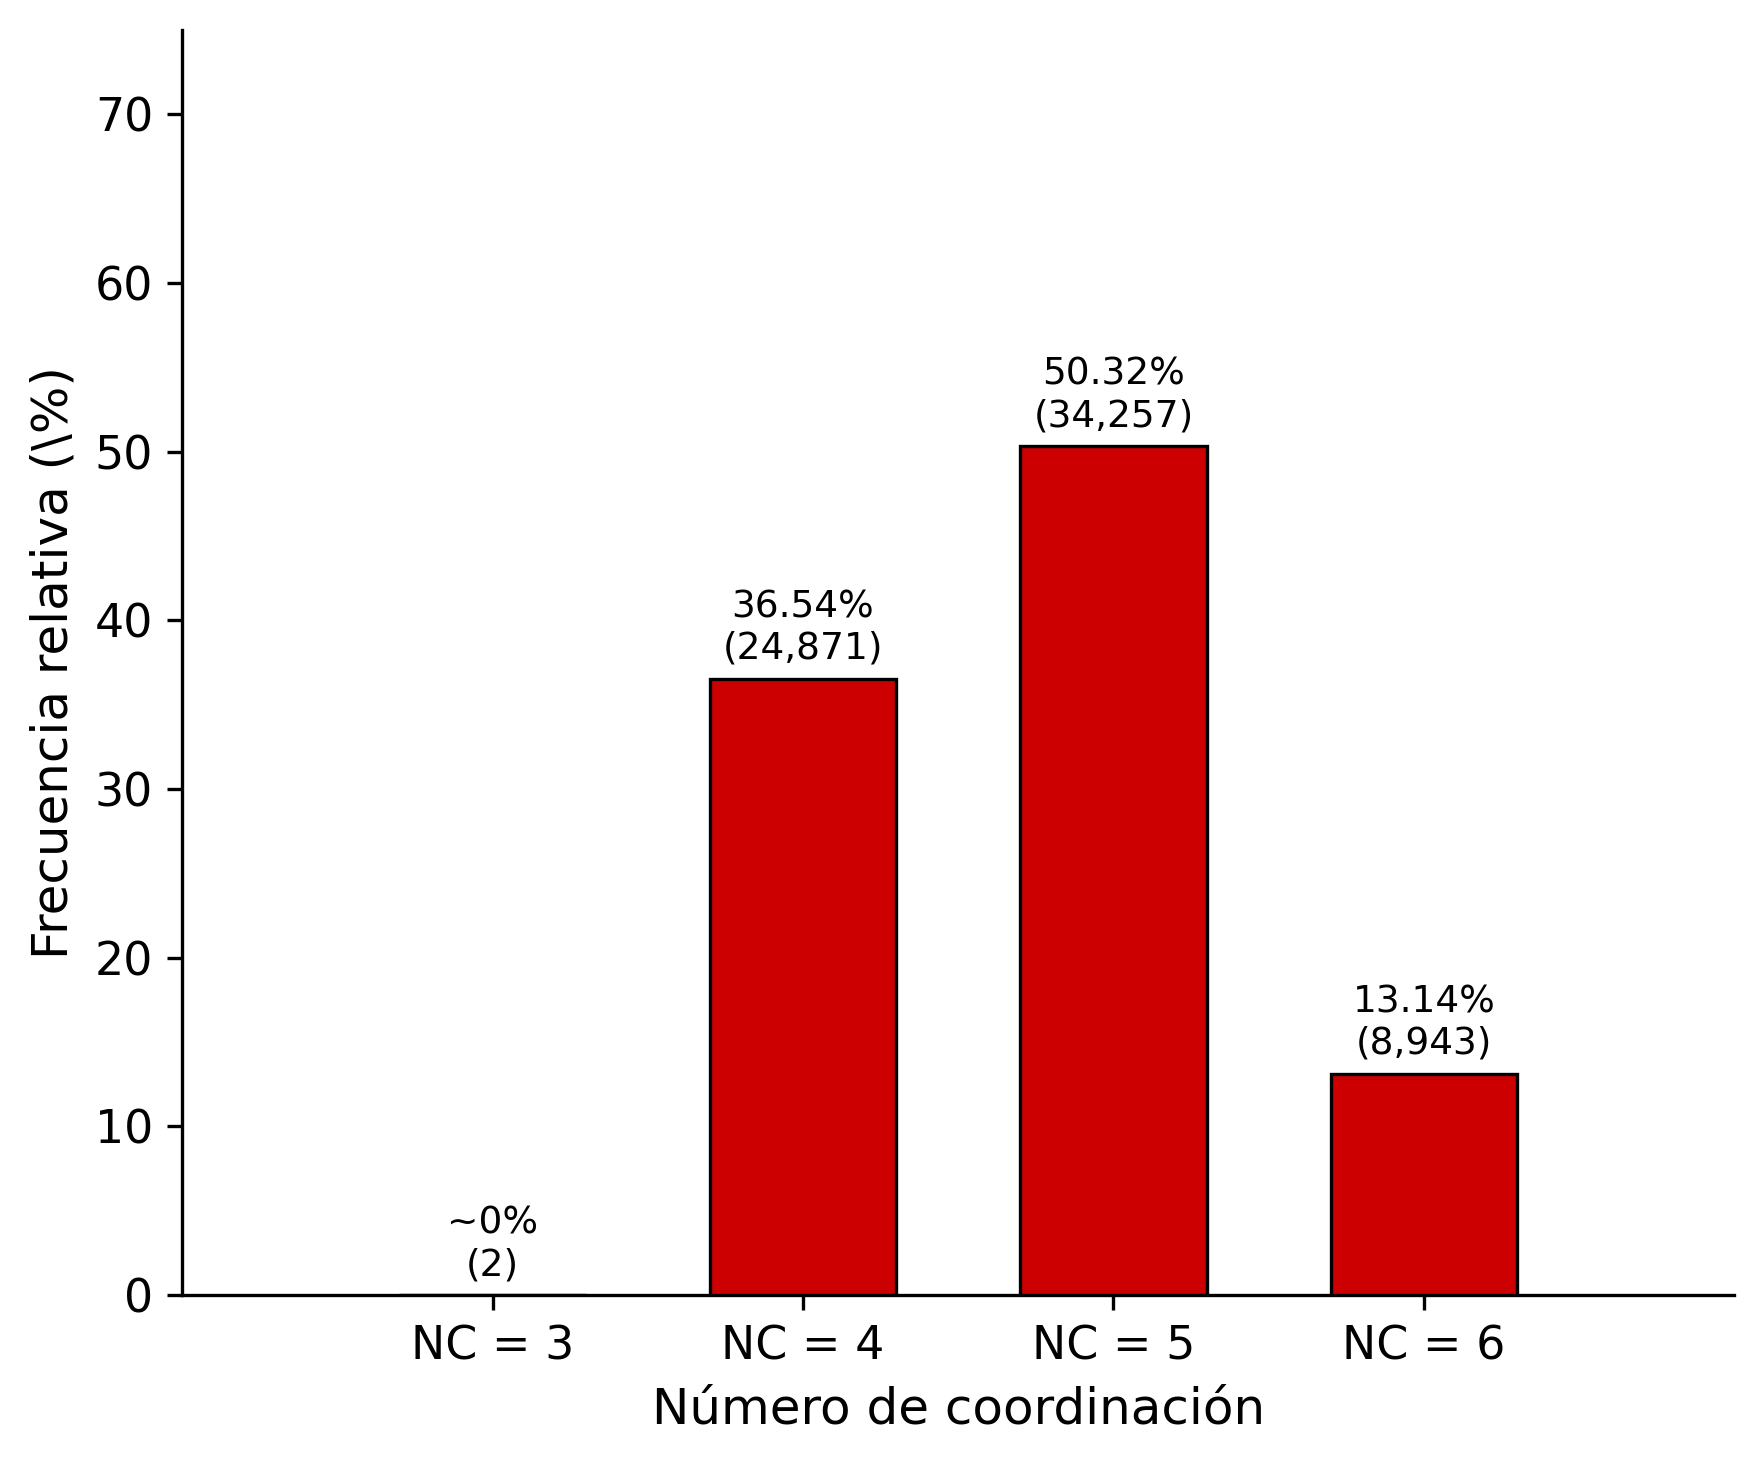
\includegraphics[width=0.5\textwidth]{Imágenes/nc_distribution_metanol.png}
    \caption[Frecuencia del número de coordinación de \ce{[Cu(CH3OH)40]^{2+}}]{Frecuencia del número de coordinación del ion obtenida a partir de la trayectoria (68\,073 frames, $r = 3.023$~\AA).}
    \label{fig:nc_distribution_methanol}
\end{figure}

\subsection*{Función de distribución angular y geometría de coordinación}

La ADF obtenida para el sistema \ce{[Cu(CH3OH)_{40}]^{2+}} se muestra en la Figura \ref{fig:adf_metanol}. Al igual que en el sistema acuoso, el perfil presenta un pico principal en $\theta \approx 87^\circ$, que recoge los ángulos ecuatoriales cis de la pirámide cuadrada, desplazados ligeramente por debajo de los $90^\circ$ ideales por efecto del movimiento térmico. El hombro extendido entre $\sim\!100^\circ$ y $\sim\!130^\circ$ agrupa los ángulos ecuatorial axial de la pirámide cuadrada ($100^\circ$--$110^\circ$) y los ángulos ecuatoriales de la bipirámide trigonal y la pirámide trigonal, próximos a $120^\circ$; su morfología aplanada, sin un máximo definido, es indicativa del intercambio continuo entre estas disposiciones geométricas a lo largo de la dinámica.

% --- ADF METANOL ---
\begin{figure}[H]
    \centering
    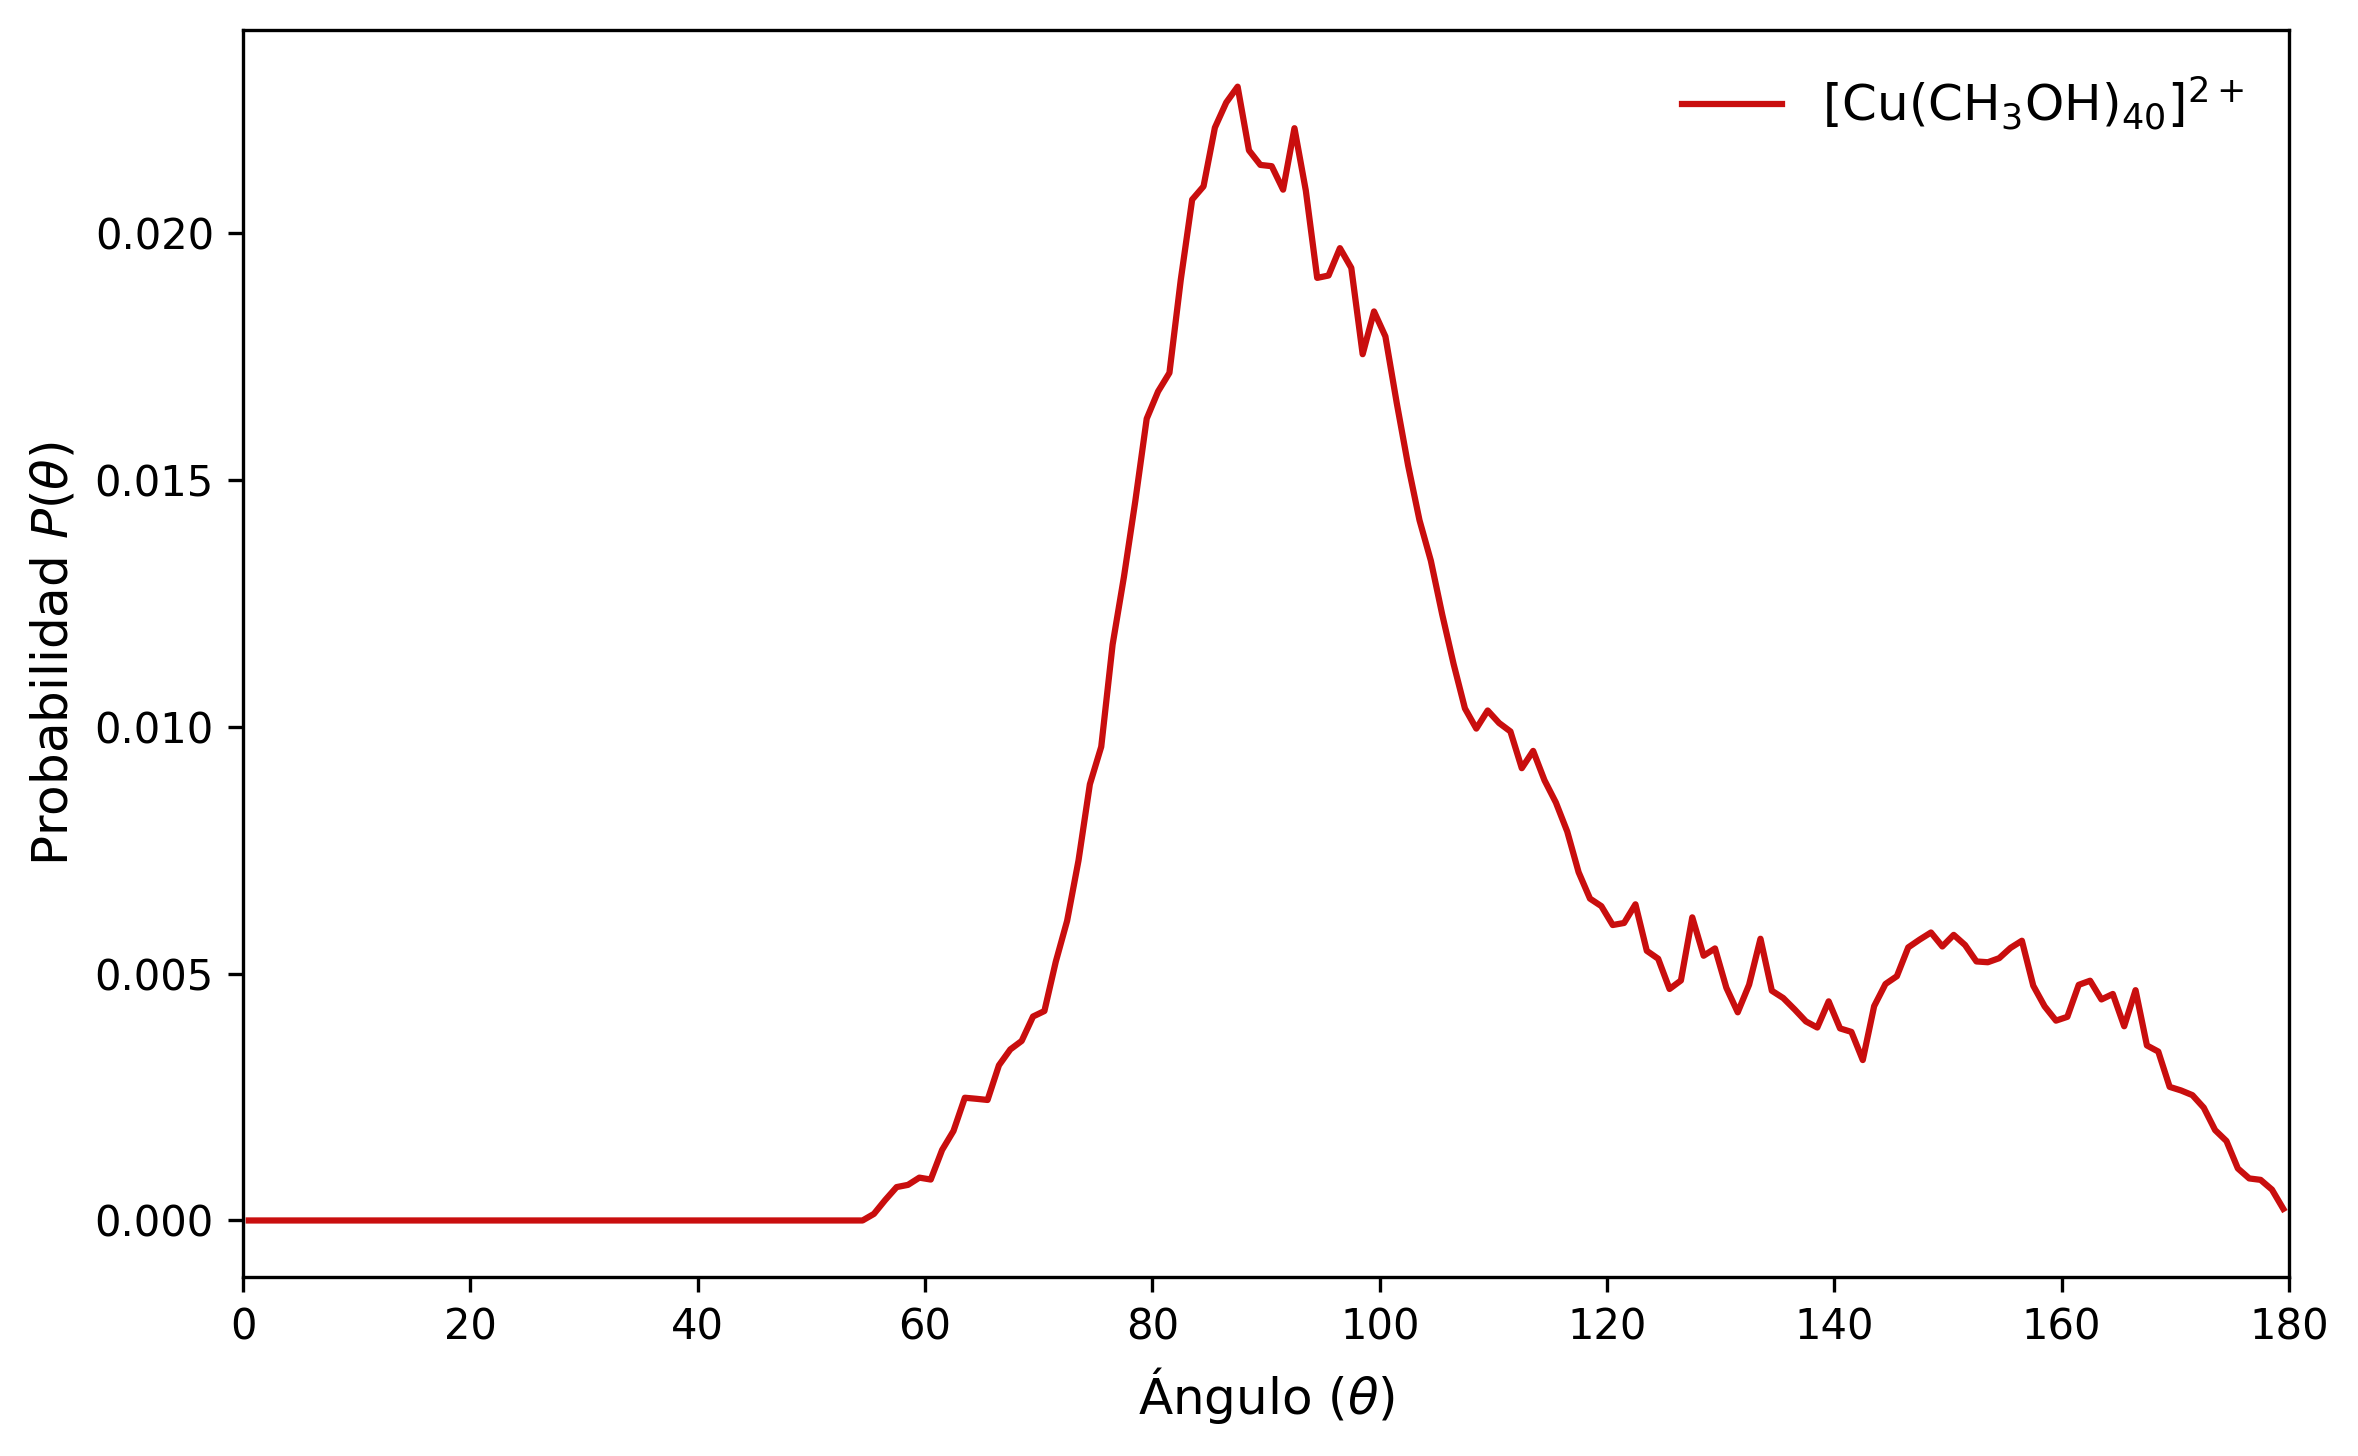
\includegraphics[width=0.95\textwidth]{Imágenes/ADF-OUTPUT-CH4O.png}
    \caption[ADF para el cúmulo \ce{[Cu(CH3OH)40]^{2+}}]{Función de distribución angular (ADF) obtenida para el sistema \ce{[Cu(CH3OH)40]^{2+}} a partir de la simulación de dinámica molecular.}
    \label{fig:adf_metanol}
\end{figure}

La diferencia más notable respecto al sistema acuoso es la presencia de un incremento en la frecuencia de ángulos a partir de $\sim\!148^\circ$. Esta zona angular únicamente puede ser poblada por pares de ligandos en disposición cuasi-trans, cuyo ángulo de referencia ideal de $180^\circ$ aparece comprimido por el movimiento térmico. Las geometrías que generan este tipo de ángulos son aquellas con coordinación elevada: la octaédrica ideal, la octaédrica distorsionada y la cuadrada plana. Esta observación es cuantitativamente consistente con el análisis del número de coordinación: en el sistema de metanol, el estado NC\,=\,6 se alcanza en el 13.14\,\% de los frames de la trayectoria, frente al 7.68\,\% registrado para el sistema acuoso. El mayor tiempo que el \ce{Cu^{2+}} permanece hexacoordinado en metanol implica una contribución proporcionalmente mayor de ángulos cuasi-trans a la ADF, lo que es directamente consistente con la función de distribución angular.

Las geometrías representativas de la primera esfera de coordinación, identificadas a partir de la inspección visual de la trayectoria, se ilustran en la Figura \ref{fig:geom_repr_metanol}.

\begin{figure}[htbp]
    \centering

    % --- Fila 1: PC y BT en cúmulo de 40 ---
    \begin{minipage}[b]{0.48\textwidth}
        \centering
        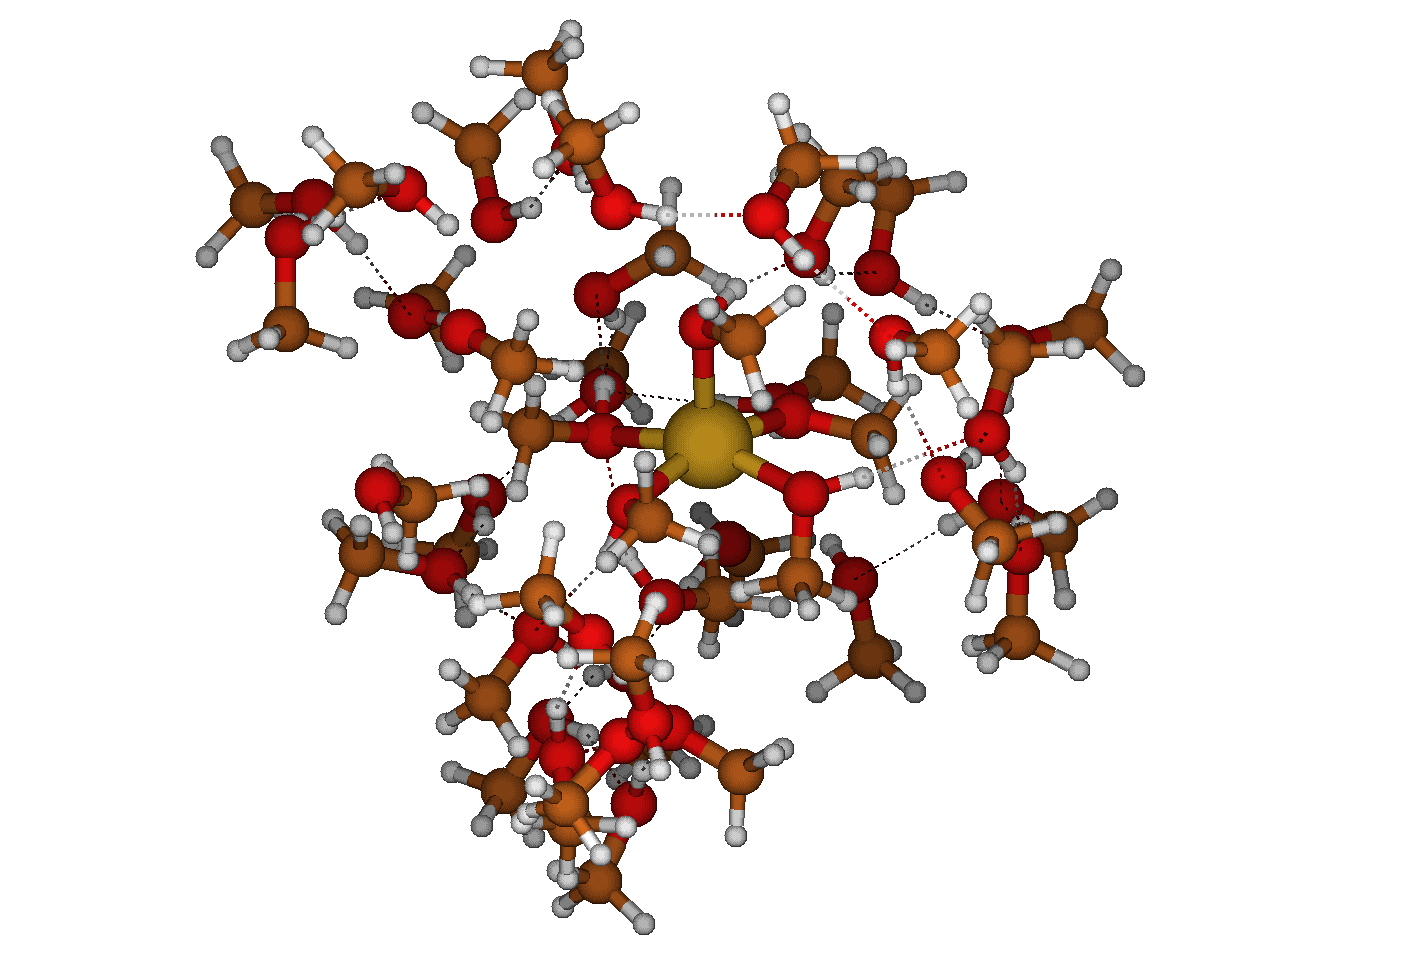
\includegraphics[width=\linewidth]{Imágenes/PC_40_m.png}
        \text{PC}
    \end{minipage}\hfill
    \begin{minipage}[b]{0.48\textwidth}
        \centering
        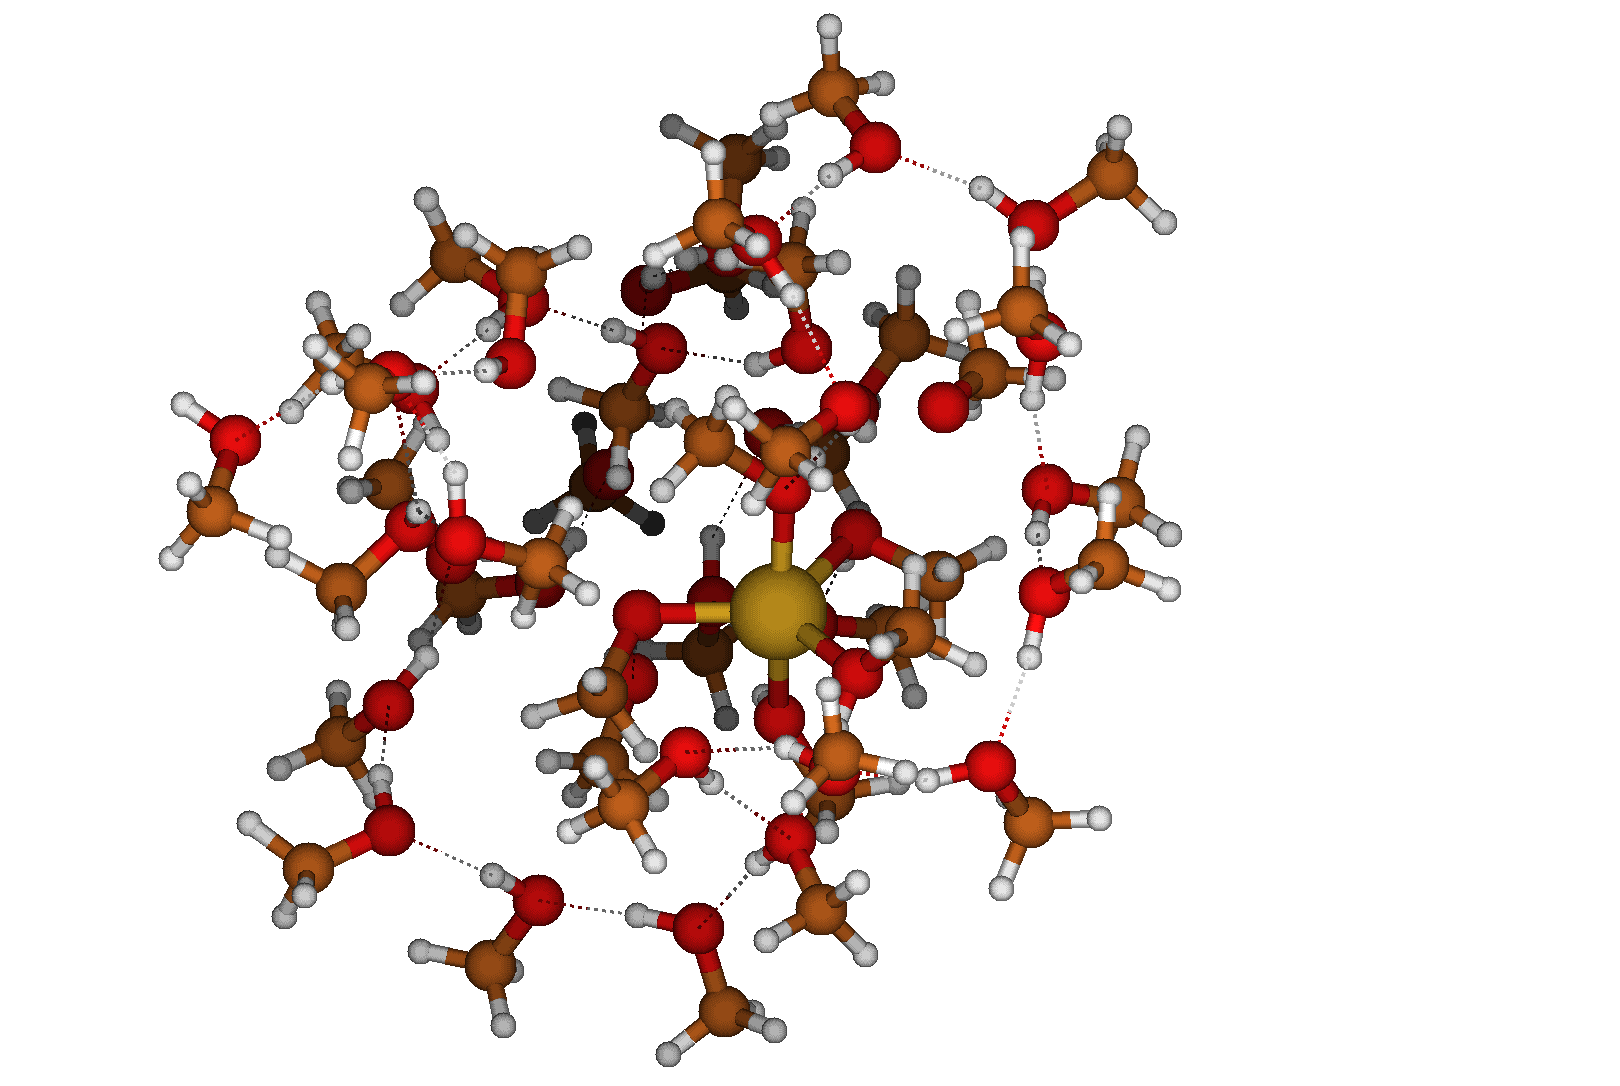
\includegraphics[width=\linewidth]{Imágenes/BT_40_m.png}
        \text{BT}
    \end{minipage}

    \vspace{0.4cm}

    % --- Fila 2: PT y OD en cúmulo de 40 ---
    \begin{minipage}[b]{0.48\textwidth}
        \centering
        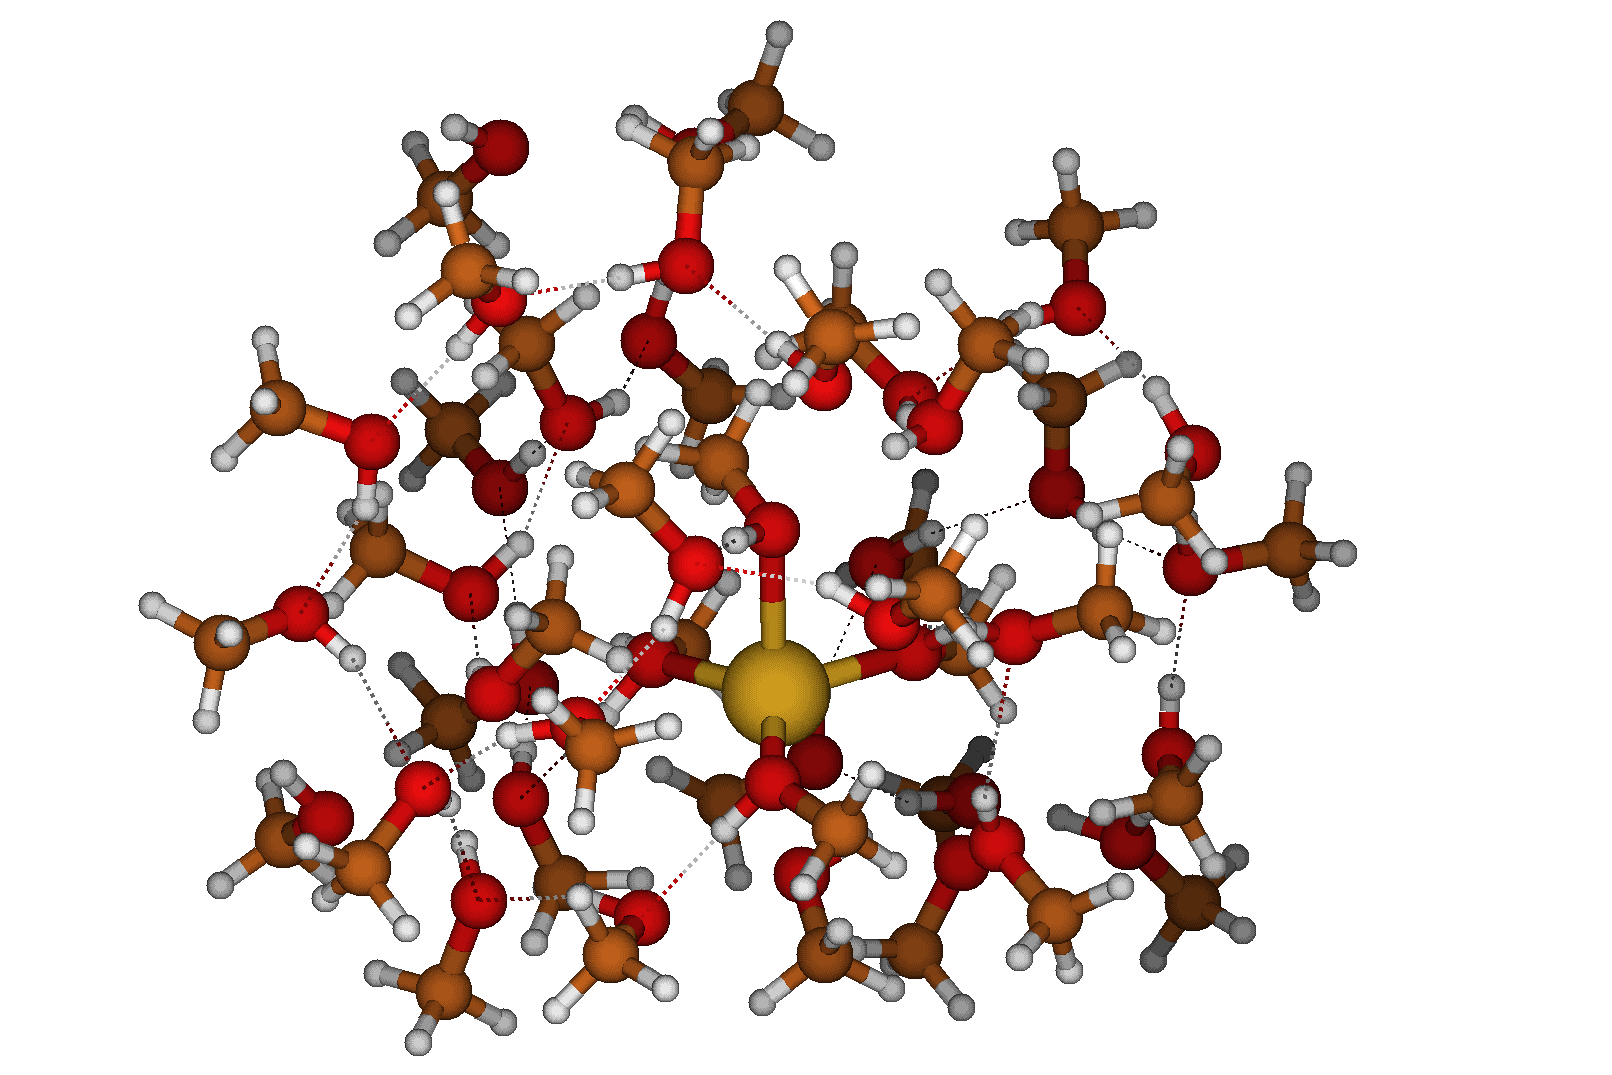
\includegraphics[width=\linewidth]{Imágenes/PT_40_m.png}
        \text{PT}
    \end{minipage}\hfill
    \begin{minipage}[b]{0.48\textwidth}
        \centering
        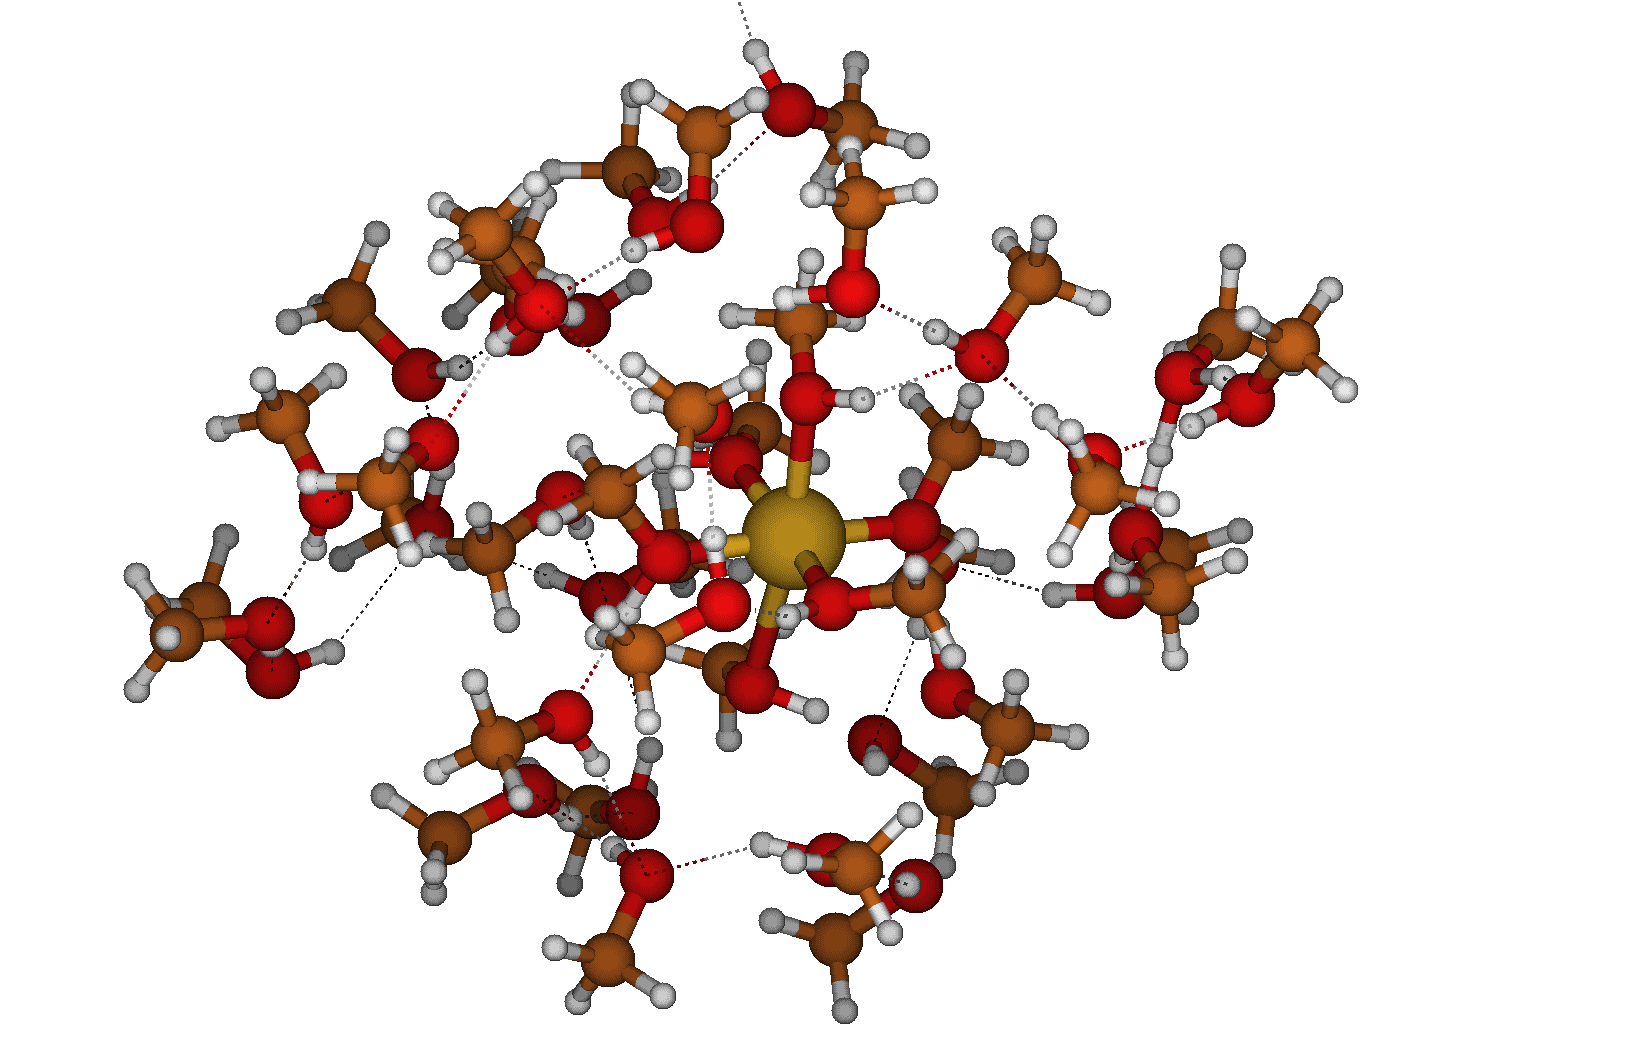
\includegraphics[width=\linewidth]{Imágenes/OD_40_m.png}
        \text{OD}
    \end{minipage}

    \vspace{0.4cm}

    % --- Fila 3: Las 4 geometrías aisladas ---
    \begin{minipage}[b]{0.23\textwidth}
        \centering
        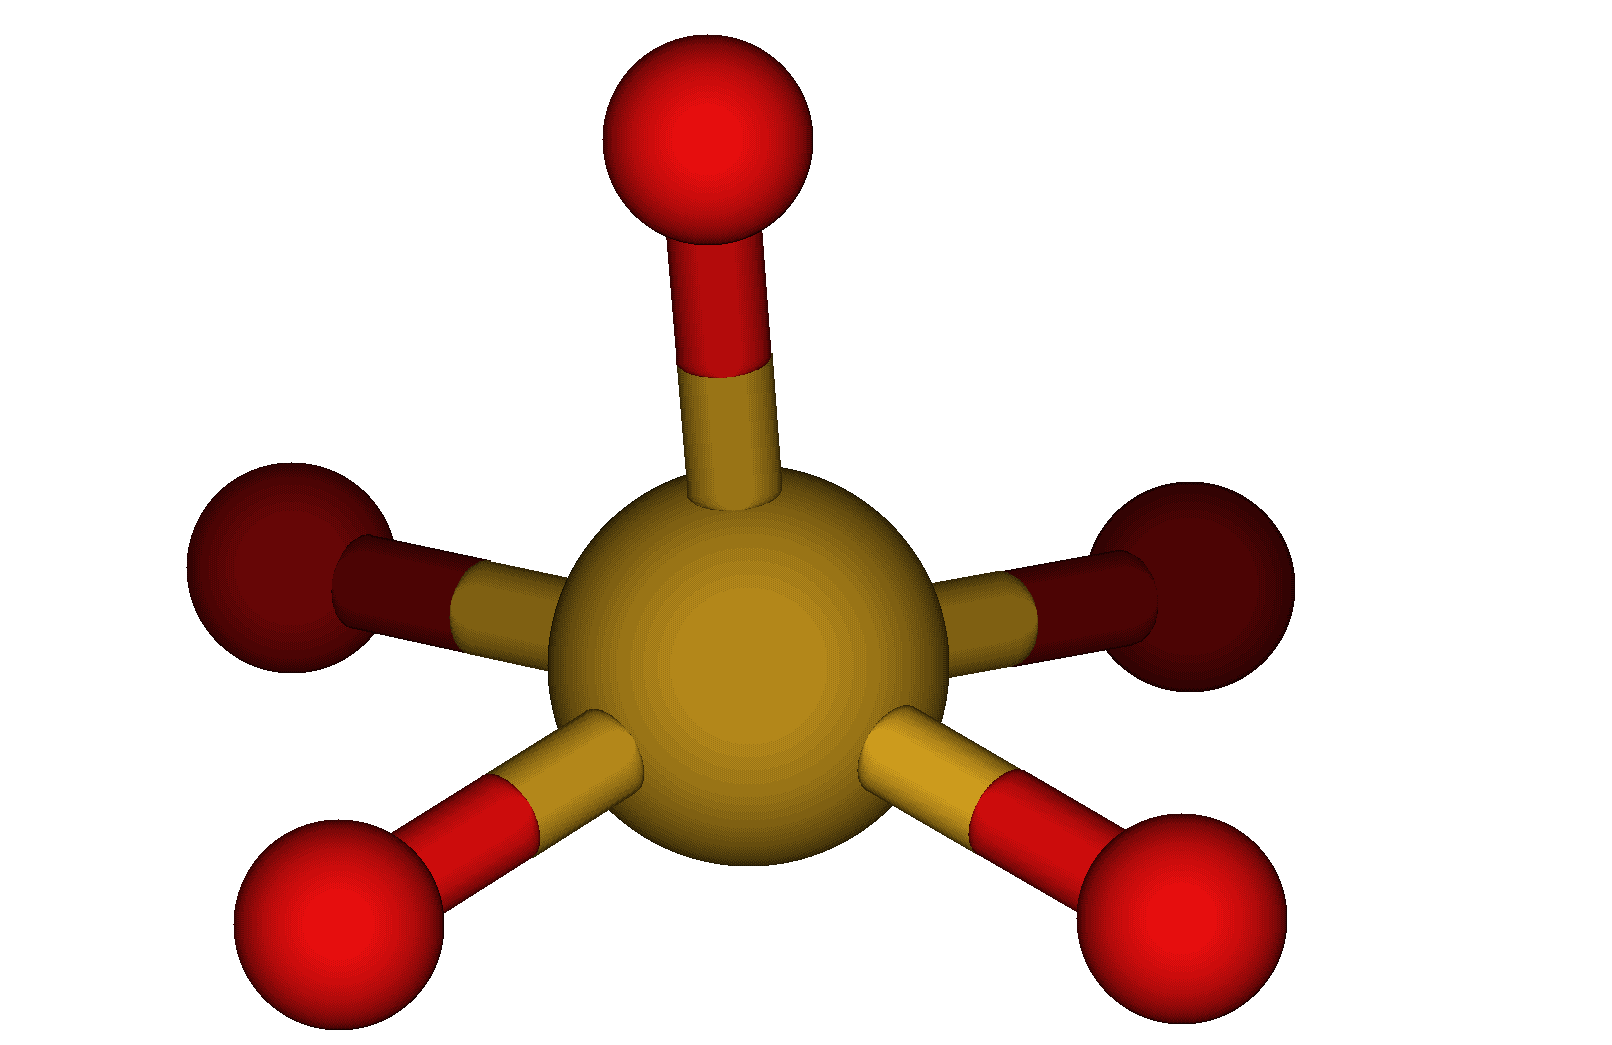
\includegraphics[width=\linewidth]{Imágenes/PC_aislada_m.png}
        \text{PC}
    \end{minipage}\hfill
    \begin{minipage}[b]{0.23\textwidth}
        \centering
        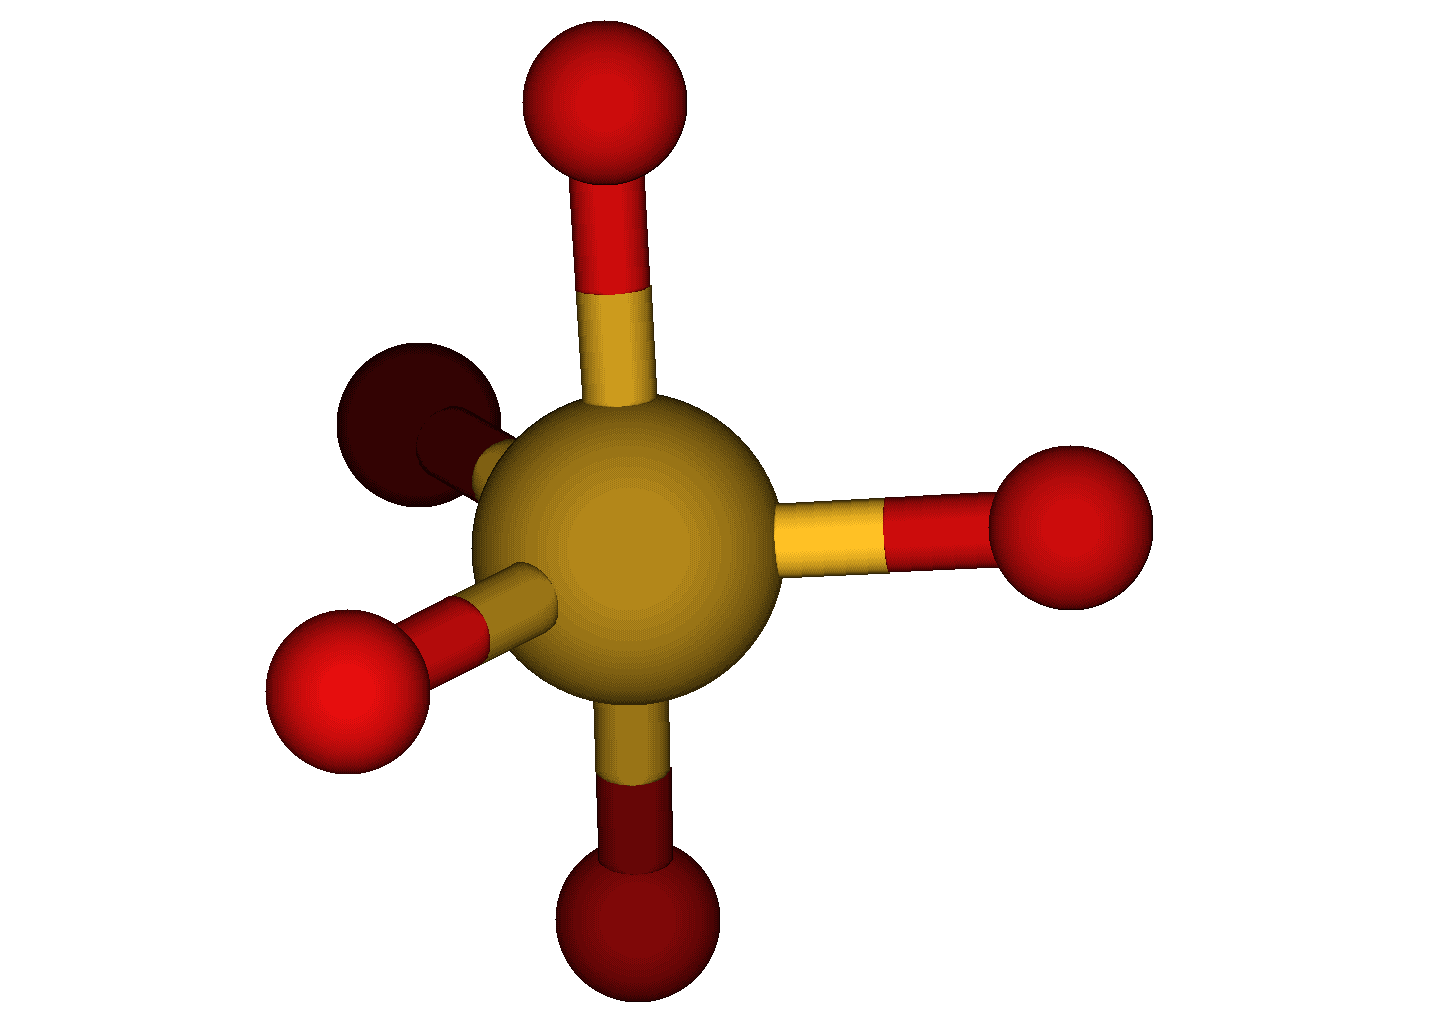
\includegraphics[width=\linewidth]{Imágenes/BT_aislada_m.png}
        \text{BT}
    \end{minipage}\hfill
    \begin{minipage}[b]{0.23\textwidth}
        \centering
        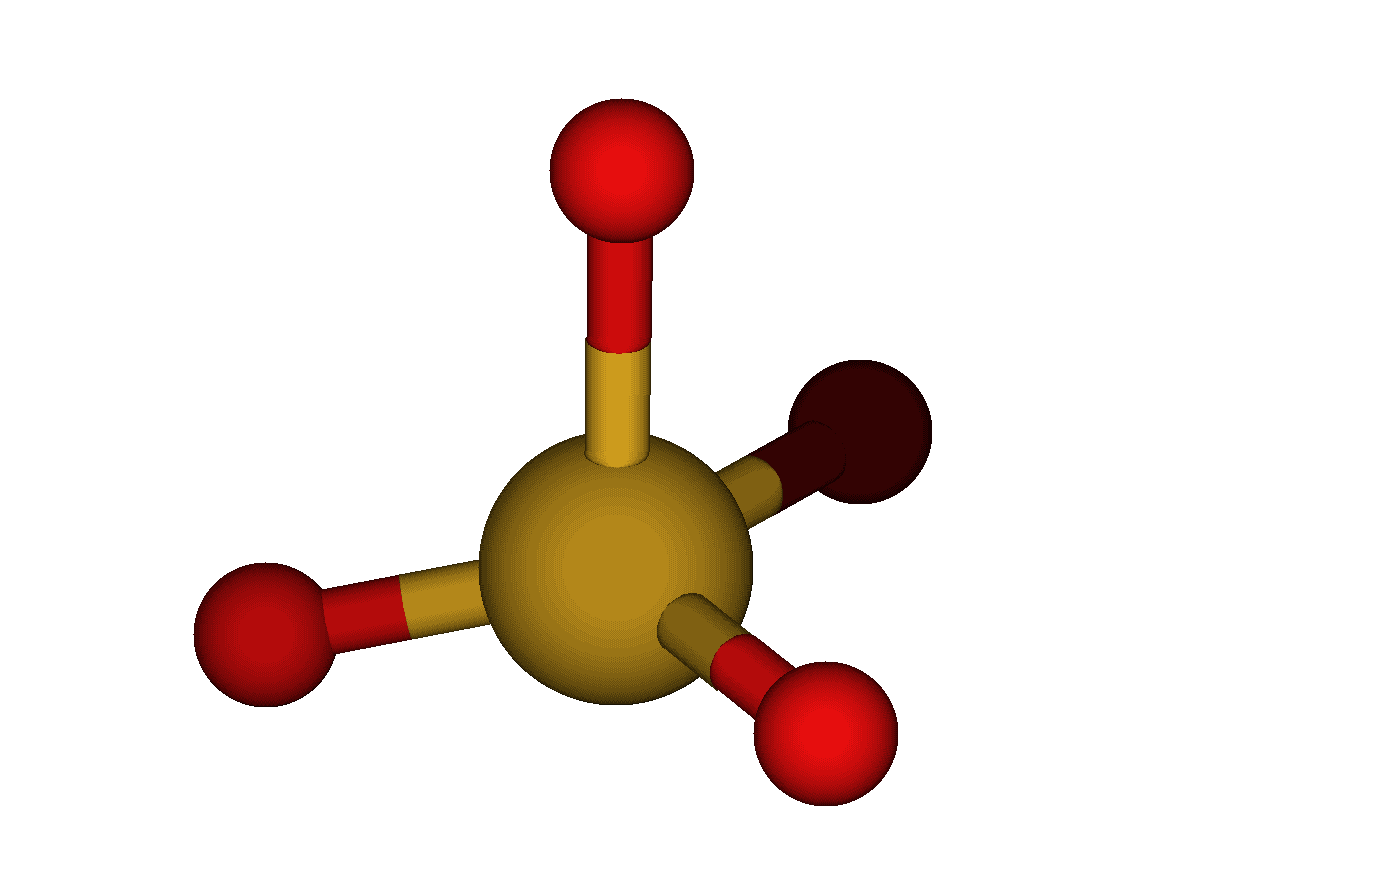
\includegraphics[width=\linewidth]{Imágenes/PT_aislada_m.png}
        \text{PT}
    \end{minipage}\hfill
    \begin{minipage}[b]{0.23\textwidth}
        \centering
        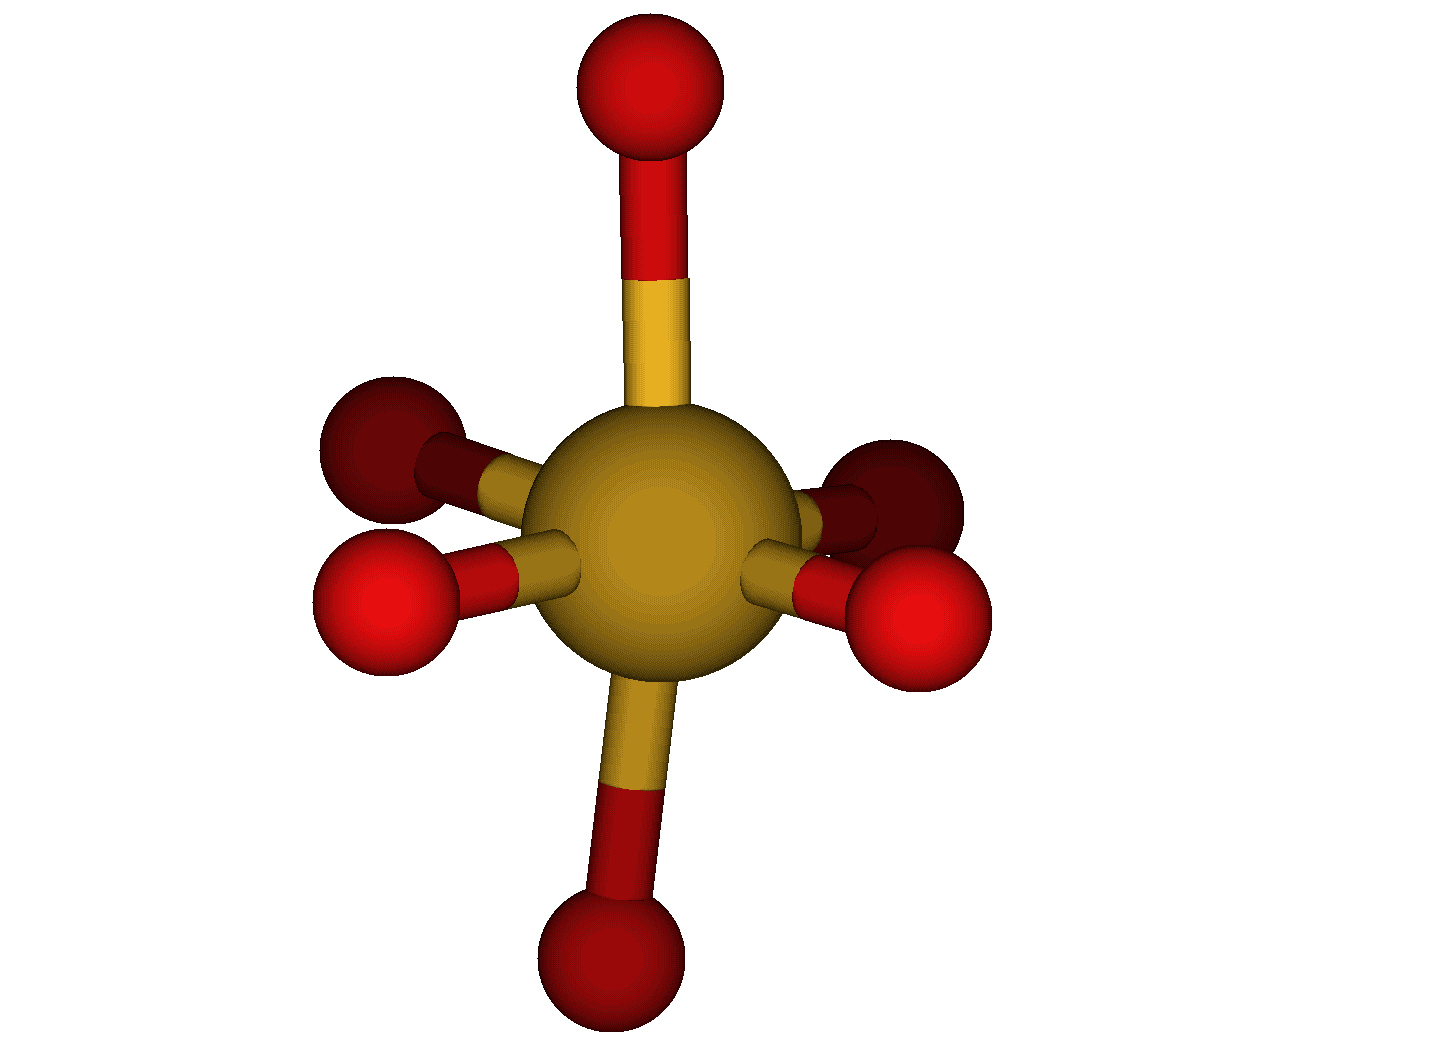
\includegraphics[width=\linewidth]{Imágenes/OD_aislada_m.png}
        \text{OD}
    \end{minipage}

    \caption[Geometrías representativas de la primera esfera, \ce{[Cu(CH3OH)_{40}]^{2+}}]{Geometrías representativas observadas en la primera esfera de
    coordinación del sistema \ce{[Cu(CH3OH)_{40}]^{2+}} extraídas de la simulación. Filas
    superior e intermedia: cada geometría representada en el cúmulo completo de 40 moléculas;
    fila inferior: primera esfera de coordinación aislada. Las geometrías predominantes son la
    \textbf{pirámide cuadrada} (PC), la \textbf{bipirámide trigonal} (BT)
    y la \textbf{pirámide trigonal} (PT), las cuales se intercambian de forma
    continua a lo largo de la dinámica. La geometría \textbf{octaédrica distorsionada} (OD)
    se incluye como referencia, pues su ocurrencia es considerablemente menor que la de las
    anteriores.}
    \label{fig:geom_repr_metanol}
\end{figure}

\subsection*{Termalización y estabilidad energética}
El análisis de la termalización y estabilidad energética se realizó siguiendo el mismo procedimiento descrito para el cúmulo \ce{[Cu(H2O)_{40}]^{2+}}. La trayectoria que se analiza es la correspondiente a la réplica C (ver Tabla \ref{tab:replicas_md}). La evolución temporal de la energía de enlace por molécula de metanol se muestra en la Figura \ref{fig:energy_metanol}.

% --- Evolución de la energía ---
\begin{figure}[H]
    \centering
    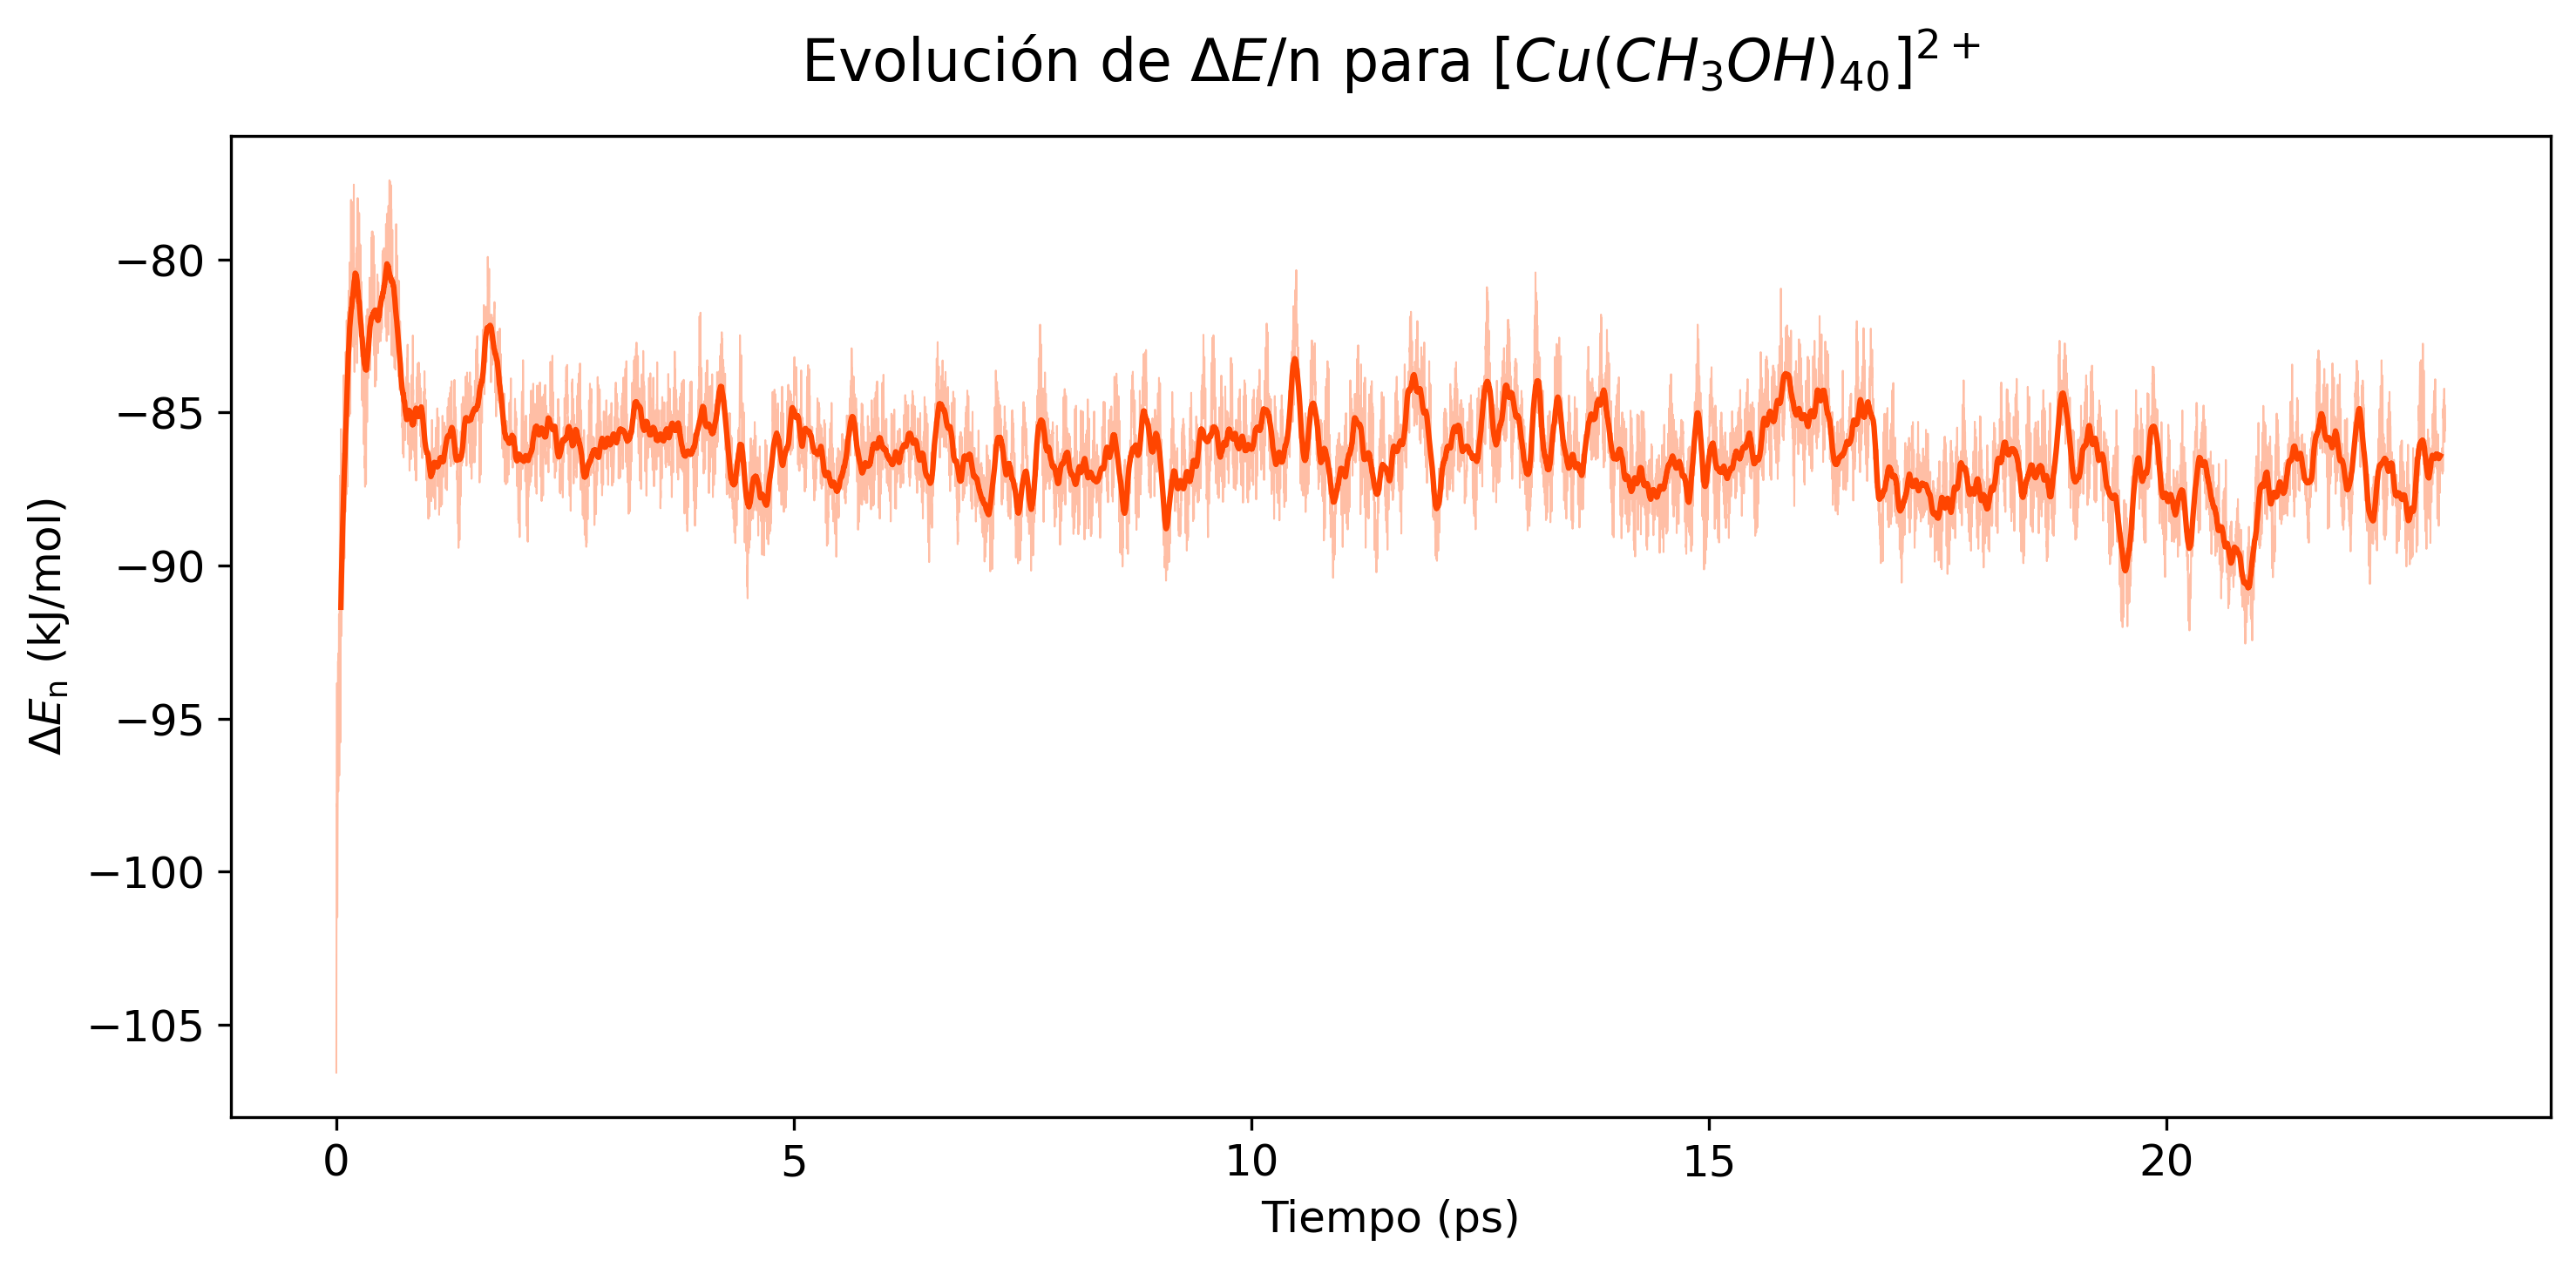
\includegraphics[width=0.95\textwidth]{Imágenes/md_energy_methanol.png}
    \caption[Evolución de la diferencia de potencial por molécula para \ce{[Cu(CH3OH)40]^{2+}}]{Evolución de la diferencia de potencial por molécula durante la simulación de dinámica molecular para el cúmulo \ce{[Cu(CH3OH)40]^{2+}}.}
    \label{fig:energy_metanol}
\end{figure}

Al igual que en el cúmulo de agua, la diferencia de potencial parte del valor correspondiente a la geometría optimizada ($-106.6$ kJ/mol) y converge a un régimen estable incluso antes de los 3 ps, lo que valida nuevamente la suficiencia del periodo de termalización empleado. El análisis estadístico de la fase de post termalización arroja $\langle \Delta E/n \rangle = -86.5 \pm 1.6$~kJ/mol por molécula de metanol, con fluctuaciones de amplitud $\sim 12$~kJ/mol y sin ninguna deriva apreciable a lo largo de la trayectoria.

\subsection*{Eventos de intercambio}

El seguimiento temporal de las distancias \ce{Cu^{2+}}--O revela que 15 de los 40 oxígenos del cúmulo residieron en la primera esfera de coordinación durante al menos un intervalo de la trayectoria ($r_\text{corte} = 3.023$~\AA), lo que evidencia la misma naturaleza dinámica del cúmulo de agua. La Figura \ref{fig:distancias_panoramica_metanol} muestra la evolución de solo 9 de estas moléculas; las 31 restantes, que nunca cruzaron el radio de corte o no son del todo relevantes, se omiten por claridad visual. A lo largo de los 23 ps totales se identificaron dos eventos de intercambio completos, descritos a continuación.

\begin{figure}[htbp]
    \centering
    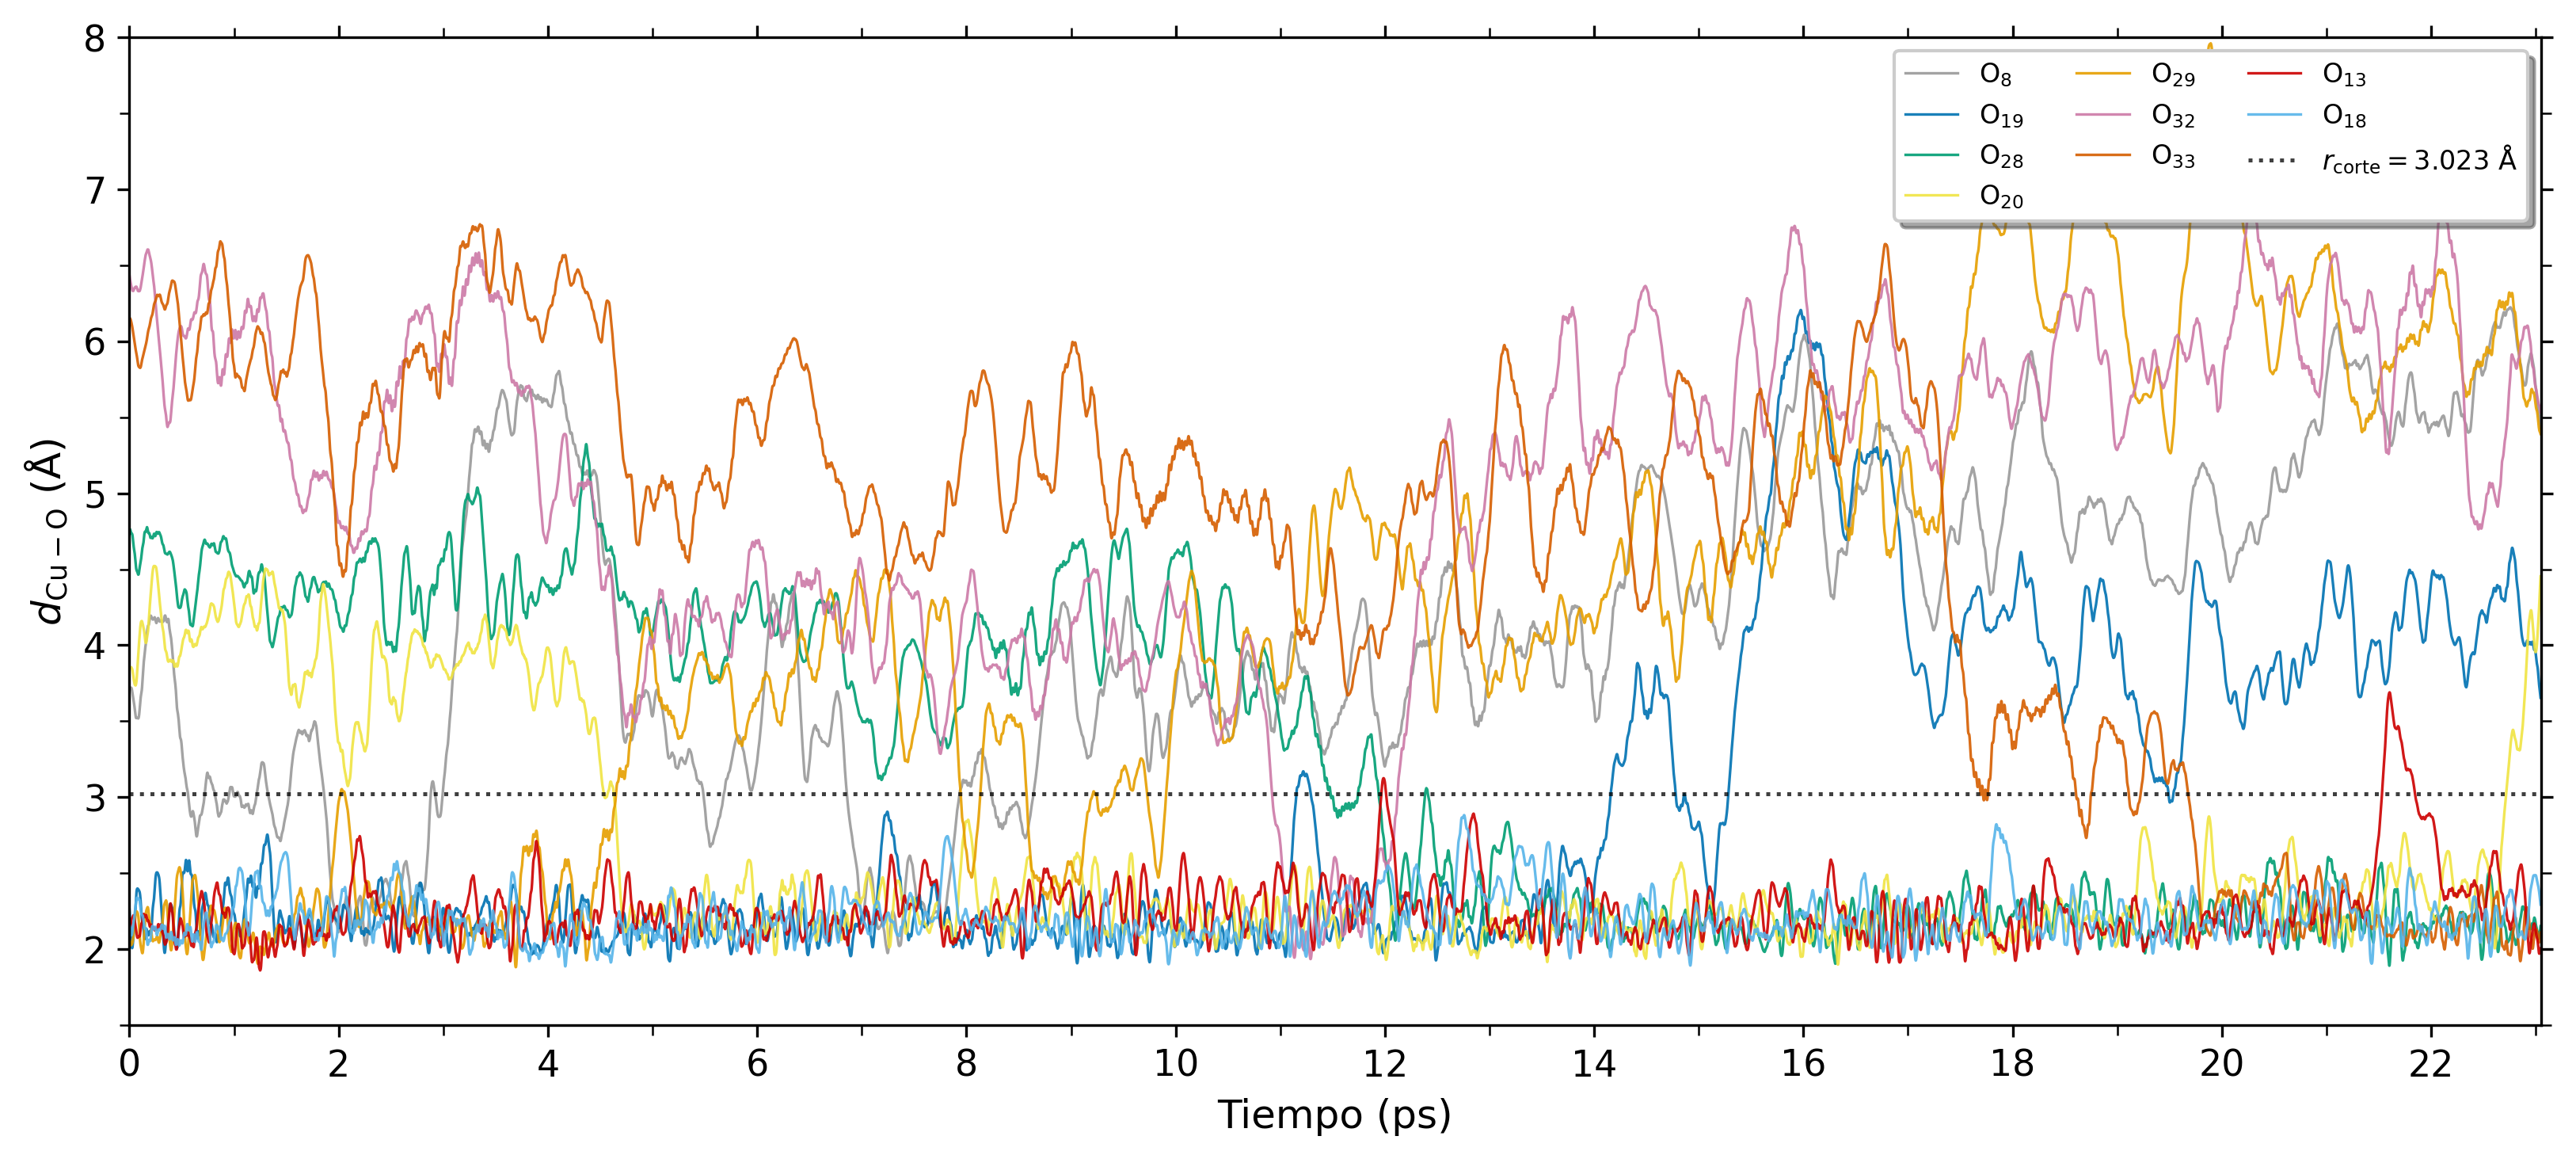
\includegraphics[width=0.95\textwidth]{Imágenes/distancias_panoramica_metanol.png}
    \caption[Evolución de distancias \ce{Cu^{2+}}--O en \ce{[Cu(CH3OH)40]^{2+}}]{Evolución temporal de las distancias \ce{Cu^{2+}}--O para las 9 moléculas de metanol de mayor interés en el cúmulo \ce{[Cu(CH3OH)_{40}]^{2+}}. La línea punteada indica el radio de corte $r_\text{corte} = 3.023$~\AA.}
    \label{fig:distancias_panoramica_metanol}
\end{figure}

El primer evento involucra a O$_{19}$ y O$_{28}$ (Figura \ref{fig:distancias_O19_O28}). Este difiere cualitativamente de los demás: la salida y la entrada no son simultáneas sino que se separan por un intervalo de aproximadamente 2 ps, lo que sugiere la formación de un estado de coordinación intermedio.

\begin{figure}[htbp]
    \centering
    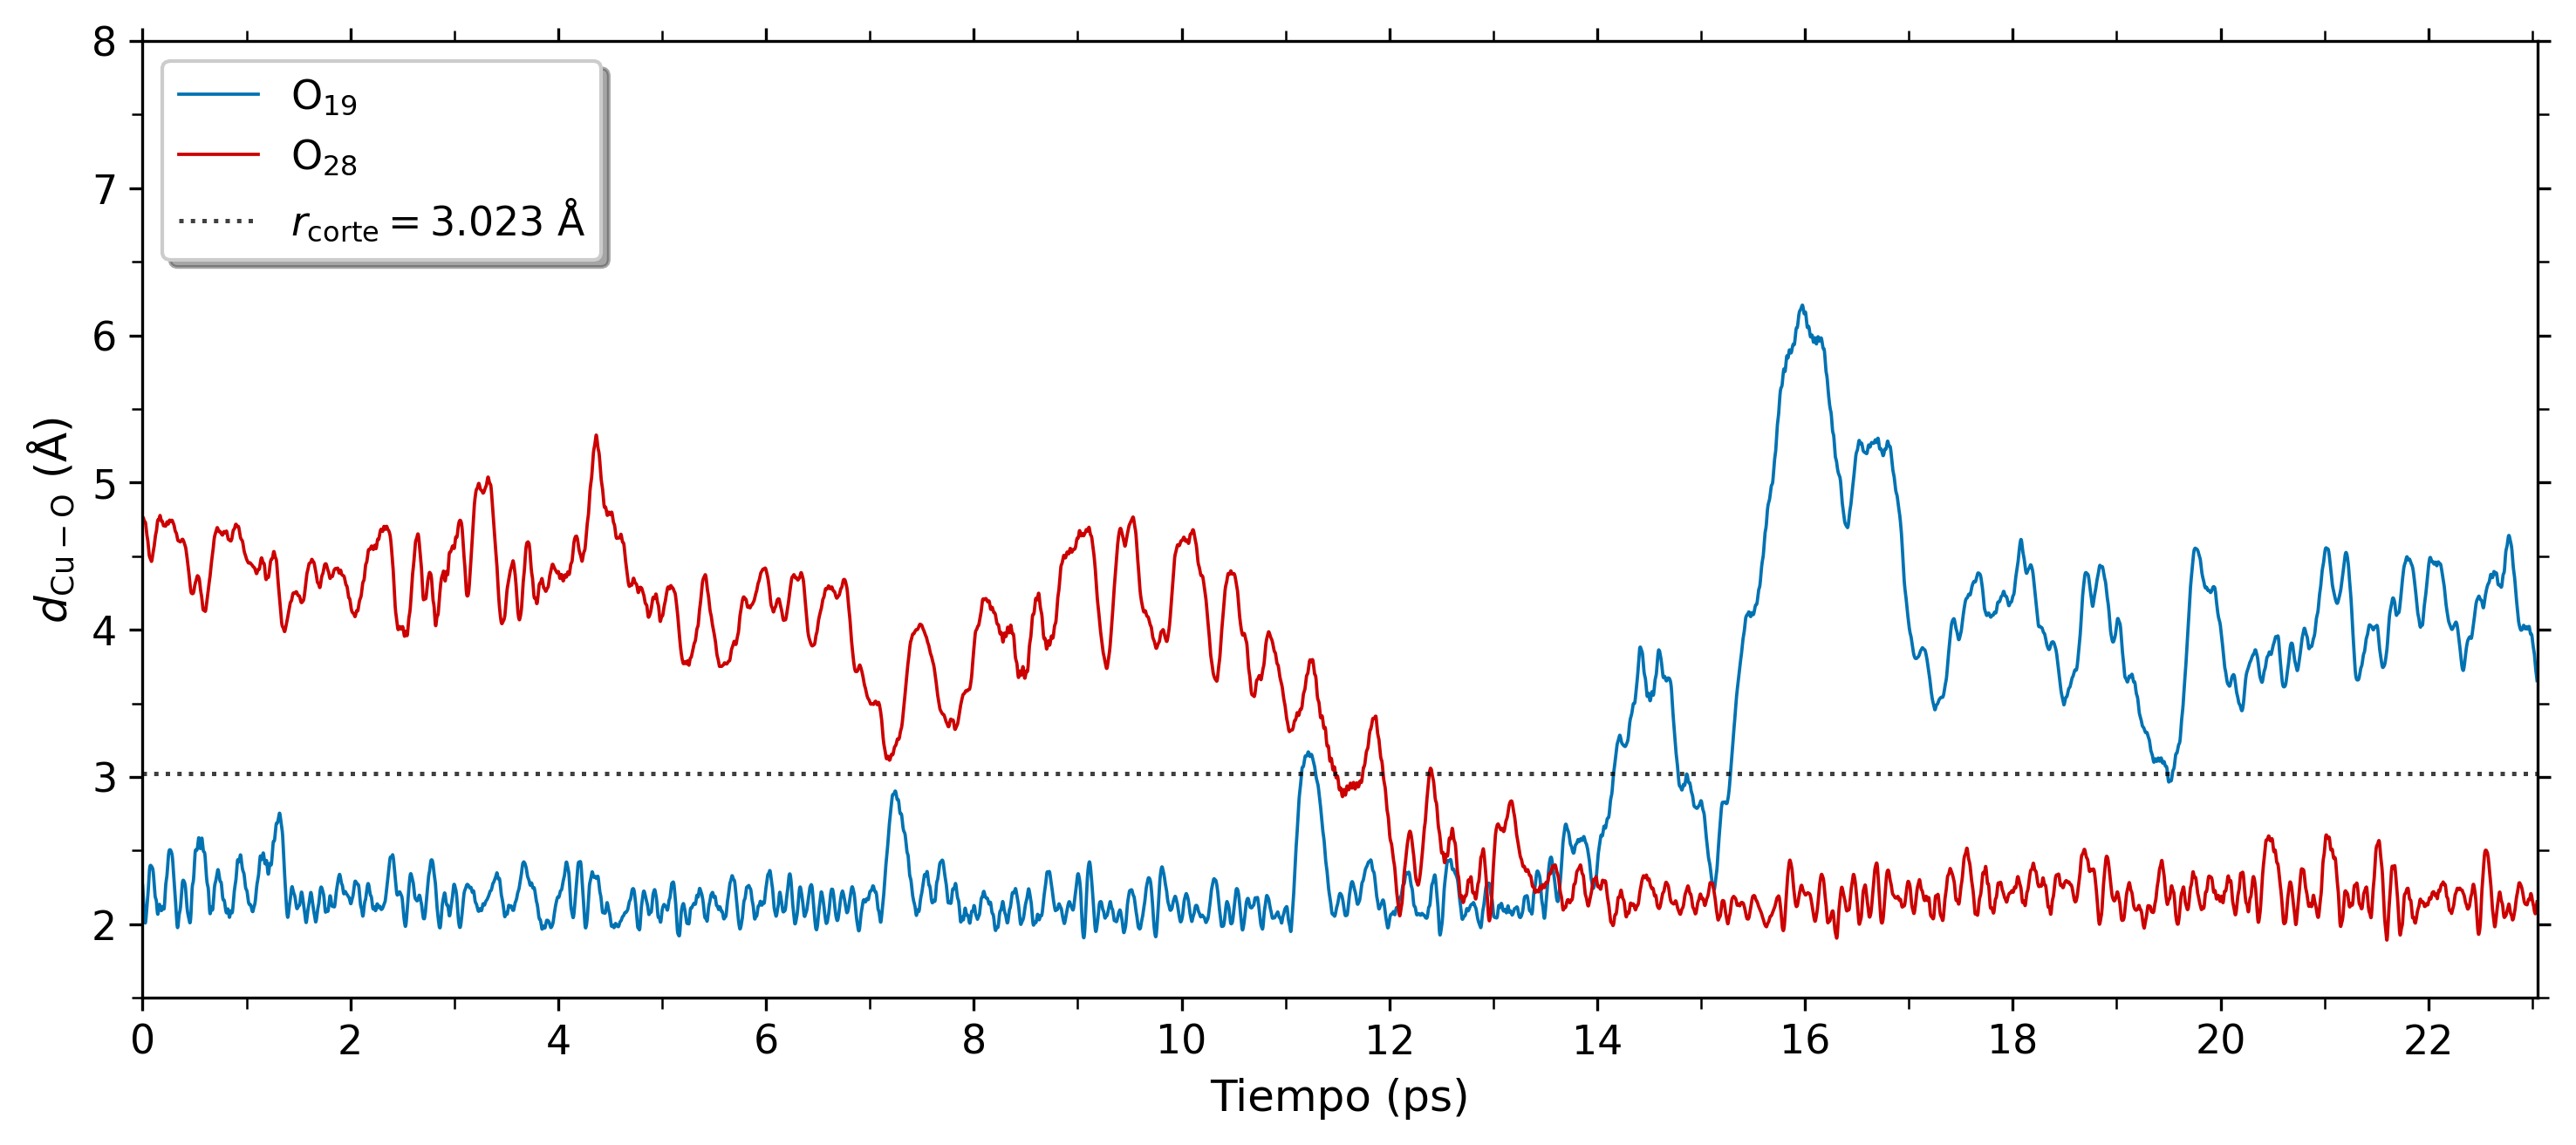
\includegraphics[width=0.95\textwidth]{Imágenes/distancias_O19_O28.png}
    \caption[Evento de intercambio O$_{19}$ $\leftrightarrow$ O$_{28}$]{Evolución temporal de las distancias \ce{Cu^{2+}}--O para O$_{19}$ y O$_{28}$. O$_{19}$. La ventana de tiempo entre la salida de O$_{19}$ y la entrada de O$_{28}$ es de aproximadamente 2 ps, lo que sugiere la formación de un estado de coordinación intermedio.}
    \label{fig:distancias_O19_O28}
\end{figure}

El segundo evento, entre O$_{20}$ y O$_{29}$ (Figura \ref{fig:distancias_O20_O29}), presenta una dinámica más típica, con la salida de O$_{29}$ seguida rápidamente por la entrada de O$_{20}$.

\begin{figure}[H]
    \centering
    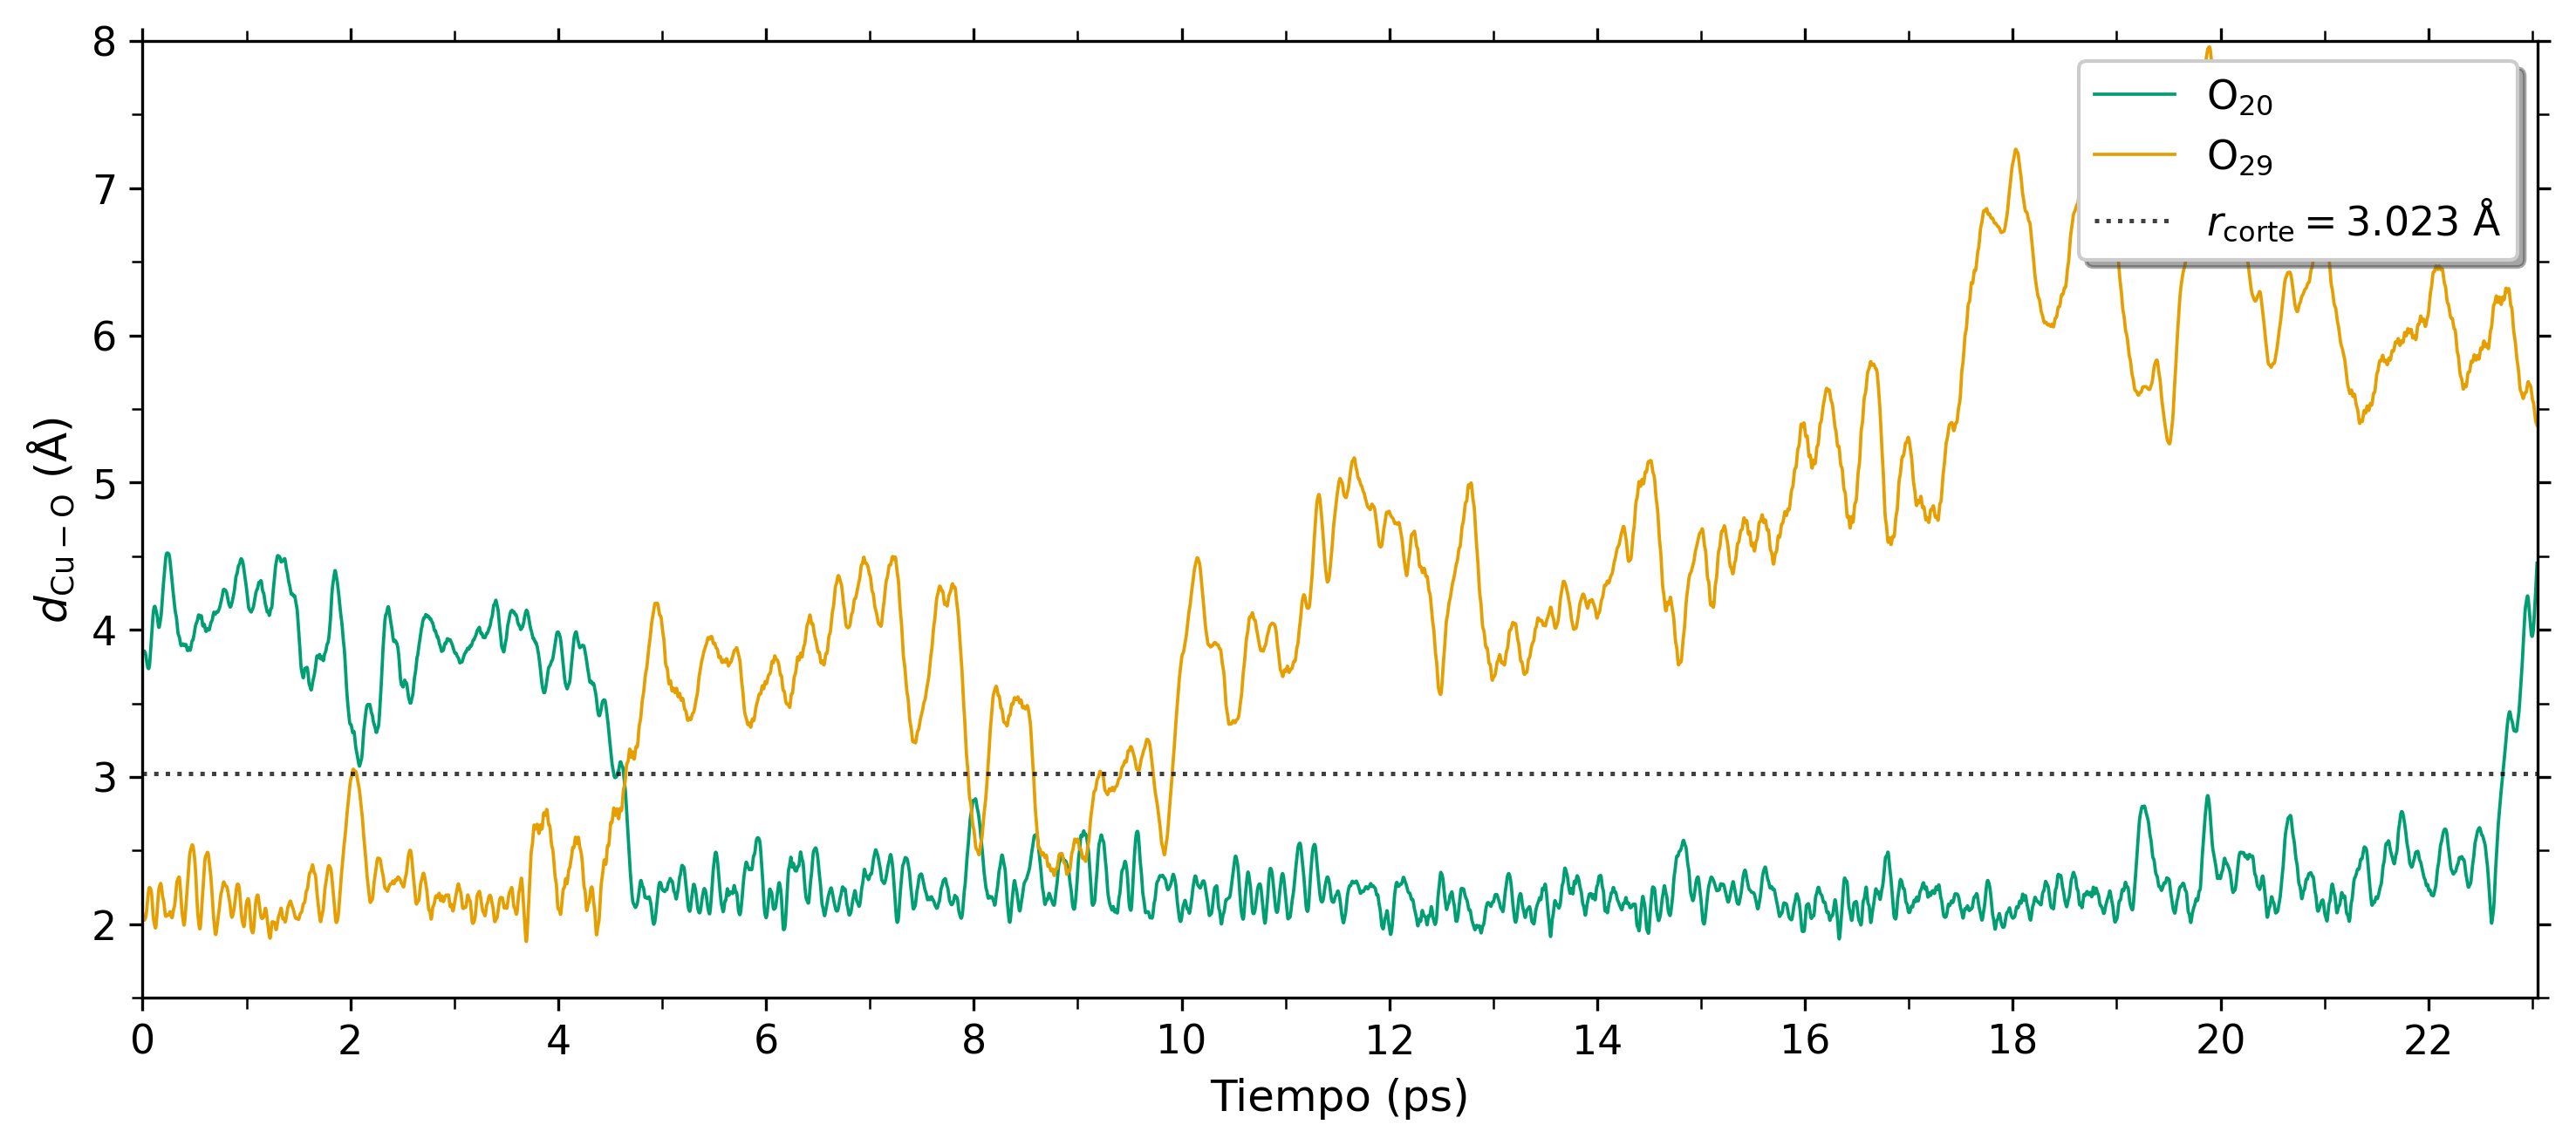
\includegraphics[width=0.95\textwidth]{Imágenes/distancias_O20_O29.png}
    \caption[Evento de intercambio O$_{20}$ $\leftrightarrow$ O$_{29}$]{Evolución temporal de las distancias \ce{Cu^{2+}}--O para O$_{20}$ y O$_{29}$. O$_{29}$. El intercambio ocurre de forma simultanea en $t \approx 4.6$ ps. La molécula de metanol con O$_{29}$ se aleja por completo del \ce{Cu^{2+}} a lo largo del resto de la simulación.}
    \label{fig:distancias_O20_O29}
\end{figure}

\section{Conclusiones}

El presente trabajo abordó la caracterización estructural y dinámica del \ce{Cu^{2+}} en nanogotas de agua y metanol mediante simulaciones BOMD con el funcional M06-2X/6-31G* y un modelo de 40 moléculas de disolvente explícito. El problema de partida fue que, a pesar de la relevancia del \ce{Cu^{2+}}, su solvatación ha sido descrita mayoritariamente a partir de cálculos estáticos y optimizaciones de geometría, muchas veces extraídas como instantáneas aisladas de trayectorias, lo que resulta insuficiente para un sistema intrínsecamente fluctuante. Bajo la premisa de que un tratamiento dinámico ab initio ofrecería una descripción más fiel del ion como un equilibrio entre geometrías, se obtuvieron las siguientes conclusiones:

\begin{enumerate}
    \item La combinación BOMD con nivel de teoría M06-2X / 6-31G* con clústeres de 40 moléculas describió exitosamente la dinámica de ambos sistemas. El funcional reprodujo la interacción ion--dipolo y los rasgos del efecto Jahn--Teller asociados a la configuración $d^9$, con energías de enlace estables y reproducibles entre réplicas: $-99.9 \pm 1.3$~kJ/mol por molécula de agua y $-86.5 \pm 1.6$~kJ/mol por molécula de metanol. Hasta donde se conoce, esta es la primera caracterización dinámica del \ce{Cu^{2+}} realizada con tal rigor teórico sobre un clúster de este tamaño para ambos solventes, lo que establece una referencia metodológica de mayor exigencia que la empleada en trabajos previos.

    \item El tratamiento dinámico reveló información inaccesible a los enfoques estáticos. En ambos disolventes, la primera esfera de coordinación no adopta una geometría única sino que fluctúa continuamente entre pirámide cuadrada, pirámide trigonal y bipirámide trigonal, con la pirámide cuadrada como disposición dominante. Los eventos de intercambio de ligandos observados, incluyendo un estado de coordinación intermedio de $\sim 2$~ps en metanol, son fenómenos que solo una descripción temporal continua puede capturar.

    \item Los parámetros estructurales convergen en una descripción coherente para ambos sistemas. La distancia \ce{Cu-O} del primer máximo de la RDF coincide en ambos disolventes (2.182~\AA), evidencia de que está dominada por la interacción ion--dipolo directa. El número de coordinación promedio es prácticamente idéntico (4.73 en agua, 4.77 en metanol), pero la descomposición del histograma revela que el estado hexacoordinado se duplica en metanol (13.14\,\% frente a 7.68\,\% en agua), diferencia que se manifiesta directamente en el aumento de ángulos cuasi-trans de la ADF. El desplazamiento del primer mínimo de la RDF (2.833~\AA{} en agua frente a 3.023~\AA{} en metanol) es consecuencia del mayor volumen estérico del metanol.

    \item La observación de eventos completos de intercambio en trayectorias de 20 ps sugiere que el tiempo de residencia de los ligandos en la primera esfera del \ce{Cu^{2+}} podría ser sensiblemente menor que los valores de 100--200~ps reportados previamente, situándose posiblemente en el régimen de decenas de picosegundos.

    \item La aportación de este trabajo es distinta para cada sistema. En el caso del \ce{Cu^{2+}} en agua, cuya solvatación ha sido objeto de un amplio debate en la literatura tanto experimental como teórica, los resultados aquí presentados no pretenden ser novedosos en su contenido, sino ofrecer una descripción más rigurosa sustentada en un nivel de teoría y un tamaño de clúster superiores a los empleados en estudios dinámicos previos. En el caso del metanol, en cambio, la caracterización dinámica del \ce{Cu^{2+}} constituye una contribución original: la literatura disponible se restringe a cálculos estáticos a 0~K, que por su naturaleza no capturan la coexistencia de geometrías, los intercambios de ligandos ni la respuesta térmica del sistema. En ese sentido, el presente trabajo no solo aporta la primera caracterización dinámica completamente ab initio del sistema, sino que muestra que dicha caracterización era necesaria para describirlo adecuadamente.
\end{enumerate}

Debe señalarse como limitación que la longitud acumulada de las trayectorias no permite un cálculo estadísticamente riguroso de los tiempos de residencia ni una cuantificación precisa de las poblaciones de cada geometría; los valores reportados deben entenderse como estimaciones sustentadas en la muestra disponible. Trabajos posteriores podrían incorporar el cálculo de espectros EXAFS para comparación directa con datos experimentales y explorar la solvatación del \ce{Cu^{2+}} en otros solventes polares.